\documentclass[9pt,a5paper,openright]{extbook}
\usepackage[utf8]{inputenc}
\usepackage[english]{babel}
\usepackage{amsthm}
\usepackage{amsmath}
\usepackage{amsfonts}
\usepackage{amssymb}
\usepackage{enumitem}
\usepackage{listings}
\usepackage{hyperref}
\usepackage{graphicx}
\usepackage{epigraph}
\usepackage{comment}
\usepackage{mathpartir}
\usepackage{subcaption}
\usepackage{multirow}
\usepackage{pdfpages}
\usepackage{colortbl}
\usepackage[chapter]{algorithm}
\usepackage{algpseudocode}
\usepackage{algorithmicx}
\usepackage{float}
\usepackage{rotating}
\usepackage{balance}
\usepackage[font=small,labelfont=bf]{caption}
\usepackage[top=2cm,bottom=1.5cm,left=2cm,right=2.5cm]{geometry}
\author{Francesco Di Giacomo}
\title{Metacasanova: a High-performance Meta-compiler for Domain-specific Languages}
\date { }

\newcommand{\tu}{\textunderscore}
\newcounter{rqCounter}
\setcounter{rqCounter}{1}

\newcommand{\researchQuestion}[1]{
  \textbf{Research question \therqCounter:} \textit{#1}
  \setcounter{rqCounter}{\therqCounter + 1}
}

\newcommand{\problemStatement}[1]{
  \textbf{Problem statement:} \textit{#1}
}

\newcommand{\psContent}{To what extent does a meta-compiler benefit the development of a domain-specific language for game development?}

\newcommand{\rqContentOne}{To what extent can a meta-compiler reduce the amount of code required to create a compiler for a domain-specific language for game development?}

\newcommand{\rqContentTwo}{How much is the performance loss introduced by the meta-compiler with respect to an implementation written in a language compiled with a traditional compiler and is this loss acceptable when considering game development?}

\newcommand{\rqContentThree}{What is the cause of the performance degradation when employing a meta-compiler and how can this be improved?}

\definecolor{scheduleGreen}{RGB}{1,168,1}

\lstset
{
	frame = single,
	breaklines = true,
	showstringspaces = false,
	basicstyle = \ttfamily\small,	
	tabsize=2,
	captionpos=b
}

\theoremstyle{definition}
\newtheorem{definition}{Definition}[chapter]

\newcommand{\AlgError}[1]{\State $\text{\textbf{error:} #1}$}
\newcommand{\AlgLet}[2]{\State \textbf{let} #1 \textbf{be} #2}


\clubpenalty = 10000
\widowpenalty = 10000
\displaywidowpenalty = 10000

\makeindex
\begin{document}
\cleardoublepage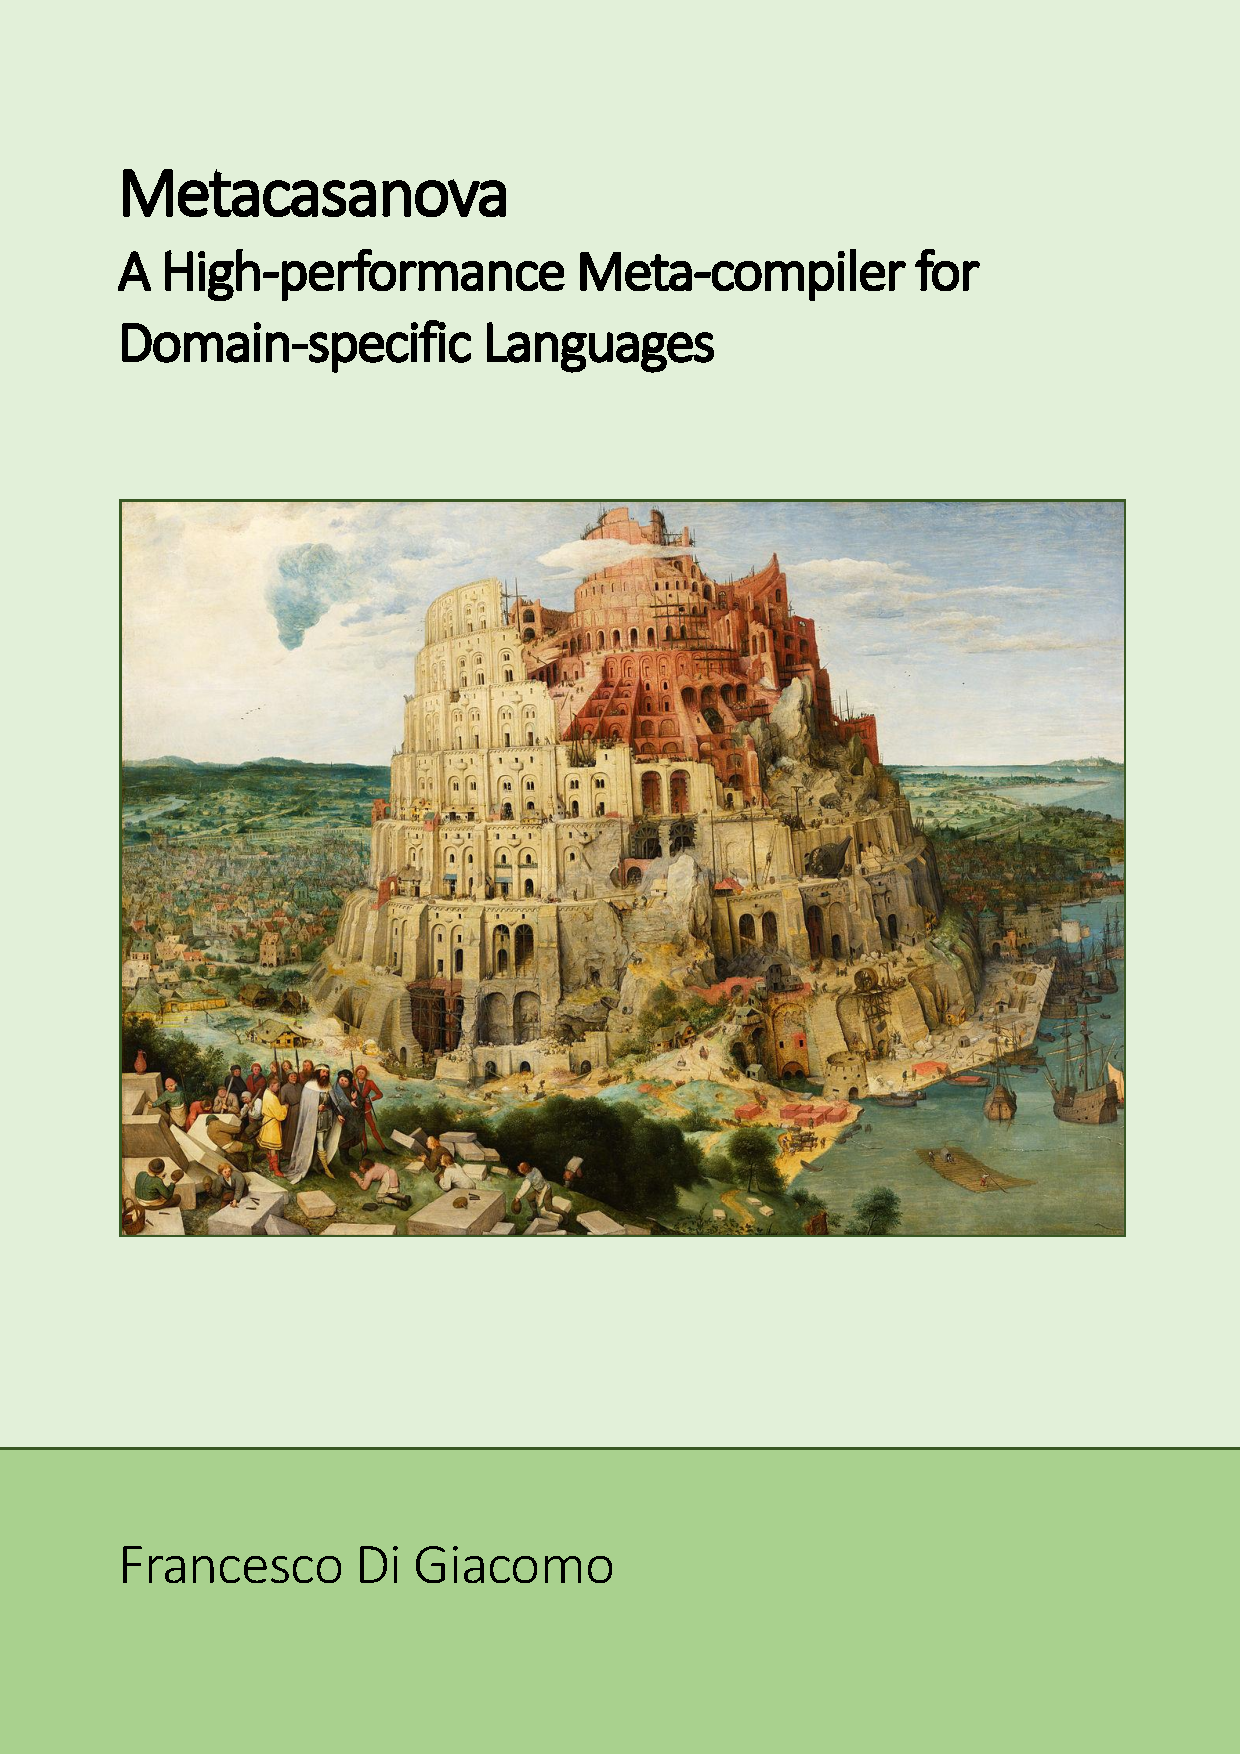
\includepdf{Extra/Cover.pdf}
\thispagestyle{empty}
\frontmatter
\pagenumbering{gobble} %remove numbering
\maketitle
%\thispagestyle{empty}
Managing the flow of time and the coordination of multiple components in games (and other highly interactive applications) is a challenging task. Therefore game development requires a lot of effort, even for (apparently) simple scenarios. To reduce the cost and effort of game development, we designed a new computer language called ``Casanova 2''. Using a case study, we demonstrate that Casanova 2 can be used to implement typical game scenario's using functional programming constructs. Our evaluation shows that it has both a high performance and a high usability.

\keywords{Game development, Casanova 2, languages, functional programming}

\newpage
%\thispagestyle{empty}
\tableofcontents

\mainmatter
\pagenumbering{arabic}
\chapter{Introduction}
\label{ch:introduction}
\epigraph{About the use of language: it is impossible to sharpen a pencil with a blunt axe. It is equally vain to try to do it with ten blunt axes instead.}{Edsger Dijkstra}
The number of programming languages available on the market has dramatically increased during the last years. The tiobe index \cite{tiobe2018}, a ranking of programming languages based on their popularity, lists 50 programming languages for 2018. This number is only a small glimpse of the real amount, since it does not take into account several languages dedicated to specific applications. This growth has brought a further need for new compilers that are able to translate programs written in those languages into executable code. The goal of this work is to investigate how the development speed of a compiler can be boosted by employing meta-compilers, programs that generalize the task performed by a normal compiler. In particular the goal of this research is creating a meta-compiler that significantly reduces the amount of code needed to define a language and its compilation steps, while maintaining acceptable performance.

This chapter introduces the issue of expressing the solution of problems in terms of algorithms in Section \ref{sec:ch1_algorithms}. Then we proceed by defining how the semi-formal definition of an algorithm must be translated into code executable by a processor (Section \ref{sec:ch1_programming_languages}). In this section we discuss the advantages and disadvantages of using different kinds of programming languages with respect to their affinity with the specific hardware architecture and the scope of the domain they target. In Section \ref{sec:ch1_compilers} we explain the reason behind compilers and we explain why building a compiler is a time-consuming task. In Section \ref{sec:ch1_metacompilers} we introduce the idea of meta-compilers as a further step into generalizing the task of compilers. In this section we also explain the requirements, benefits, and the relevance as a scientific topic. Finally in Section \ref{sec:ch1_problem_statement} we formulate the problem statement and the research questions that this work will answer.

\section{Algorithms and problems}
\label{sec:ch1_algorithms}
Since the ancient age, there has always been the need of describing the sequence of activities needed to perform a specific task \cite{barbin2012history}, to which we refer with the name of \textit{Algorithm}. The allegedly most ancient known example of this dates back to the Ancient Greek, when Hero invented an algorithm to perform the factorization and the approximation of the square root, discovered also by other civilizations \cite{ bailey2012ancient, smith1923history} . Regardless of the specific details of each algorithm, one needs to use some kind of language  to define the sequence of steps to perform. In the past people used natural language to describe such steps but, with the advent of the computer era, the choice of the language has been strictly connected with the possibility of its implementation. Natural languages are not suitable for the implementation, as they are known to be verbose and ambiguous \cite{church1982coping, resnik1999semantic}. For this reason, several kind of formal solutions have been employed, which are described below.

\subsubsection*{Flow charts}
A flow chart is a diagram where the steps of an algorithm are defined by using boxes of different kinds, connected by arrows to define their ordering in the sequence. The boxes are rectangular-shaped if they define an \textit{activity} (or processing step), while they are diamond-shaped if they define a \textit{decision}. A rectangle with rounded corners denotes the initial step. An example of a flow chart describing how to sum the numbers in a sequence is described in Figure \ref{fig:ch1_flow_chart}.

\begin{figure}
	\centering
	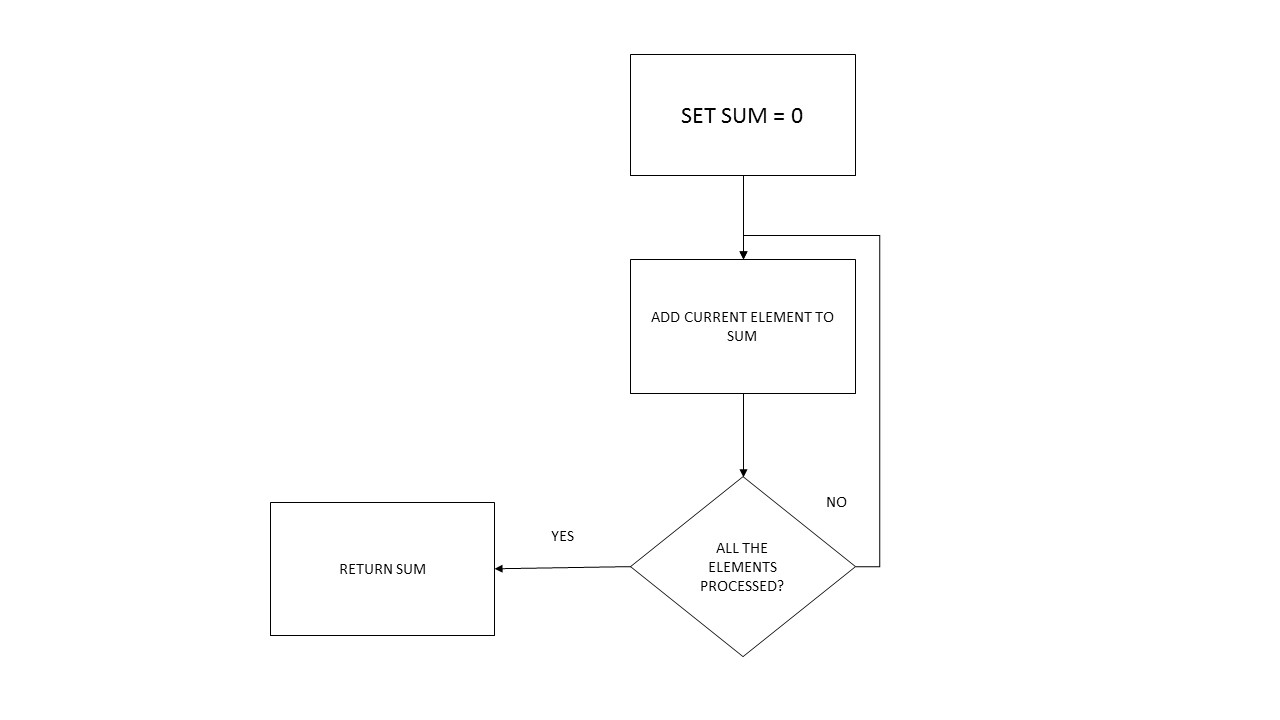
\includegraphics[width = \textwidth]{Figures/flow_chart}
	\caption{Flow chart for the sum of a sequence of numbers}
	\label{fig:ch1_flow_chart}
\end{figure}

\subsubsection*{Pseudocode}
Pseudocode is a semi-formal language that might contain also statements expressed in natural language and omits system specific code like opening file writers, printing messages on the standard output, or even some data structure declaration and initialization. It is intended mainly for human reading rather than machine reading. The pseudocode to sum a sequence of numbers is shown in Algorithm \ref{alg:ch1_pseudocode}.

\begin{algorithm}
	\caption{Pseudocode to perform the sum of a sequence of integer numbers}
	\label{alg:ch1_pseudocode}
	\begin{algorithmic}
		\Function{SumIntegers}{$l \text{ list of integers}$}
			\State $sum \gets 0$
			\ForAll {$x \text{ in } l$}
				\State $sum \gets sum + x$
			\EndFor
			\State \Return $sum$
		\EndFunction
	\end{algorithmic}
\end{algorithm}

\subsubsection*{Advantages and disadvantages}
Using flow charts or pseudo-code has the advantage of being able to define an algorithm in a way which is very close to the abstractions employed when using natural language: a flow chart combines both the use of natural language and a visual interface to describe an algorithm, pseudo-code allows to employ several abstractions and even define some steps in terms of natural language. The drawback of these two formal representations is that, when it comes to the implementation, the definition of the algorithm must be translated by hand into code that the hardware is able to execute. This could be done by implementing the algorithm in a low-level or high-level programming language. This process affects at different levels how the logic of the algorithm is presented, as explained further.

\section{Programming languages}
\label{sec:ch1_programming_languages}
A programming language is a formal language that is used to define instructions that a machine, usually a computer, must perform in order to produce a result through computation \cite{mordechai1996, narasimhan1967programming, oxford2008}. There is a wide taxonomy used to classify programming languages depending on their use \cite{kelleher2005lowering, myers1986visual, myers1990taxonomies}, but all can be grouped according to two main characteristics: the level of abstraction, or how close to the specific targeted hardware they are, and the domain, which defines the range of applicability of a programming language. In the following sections we give an exhaustive explanation of the aforementioned characteristics.

\subsection{Low-level programming languages}
\label{subsec:ch1_ll_languages}
A low-level programming language is a programming language that provides little to no abstraction from the hardware architecture of a processor. This means that it is strongly connected with the instruction set of the targeted machine, the set of instructions a processor is able to execute. These languages are divided into two sub-categories: \textit{first-generation} and \textit{second-generation} languages:

\subsubsection*{First-generation languages}
\textit{Machine code} falls into the category of first-generation languages. In this category we find all those languages that do not require code transformations to be executed by the processor. These languages were used mainly during the dawn of computer age and are rarely employed by programmers nowadays. Machine code is made of stream of binary data, that represents the instruction codes and their arguments \cite{guide2011intel, seal2001arm}. Usually this stream of data is treated by programmers in hexadecimal format, which is then remapped into binary code. The programs written in machine code were once loaded into the processor through a front panel, a controller that allowed the display and alteration of the registers and memory (see Figure \ref{fig:ch1_front_panel}). An example of machine code for a program that computes the sum of a sequence of integer numbers can be seen in Listing \ref{lst:ch1_machine_code}.

\begin{figure}
	\centering
	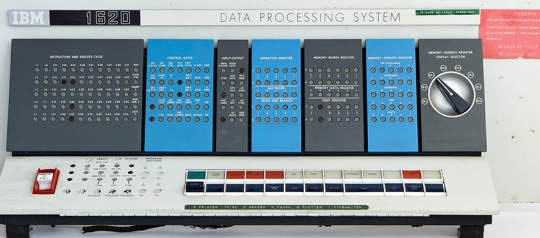
\includegraphics[width = \textwidth]{Figures/ch1_front_panel}
	\caption{Front panel of IBM 1620}
	\label{fig:ch1_front_panel}
\end{figure}

\begin{minipage}{\linewidth}
\begin{lstlisting}[numbers = left, caption = Machine code to compute the sum of a sequence of numbers, label = lst:ch1_machine_code]
 00075	c7 45 b8 00 00
 00 00
 0007c	eb 09	
 0007e	8b 45 b8
 00081	83 c0 01
 00084	89 45 b8
 00087	83 7d b8 0a
 0008b	7d 0f
 0008d	8b 45 b8
 00090	8b 4d c4
 00093	03 4c 85 d0
 00097	89 4d c4
 0009a	eb e2
\end{lstlisting}
\end{minipage}

\subsubsection*{Second-generation languages}
The languages in this category provides an abstraction layer over the machine code by expressing processor instructions with mnemonic names both for the instruction code and the arguments. For example, the arithmetic sum instruction \texttt{add} is the mnemonic name for the instruction code \texttt{0x00} in \texttt{x86} processors. Among these languages we find \textit{Assembly}, that is mapped with an \textit{Assembler} to machine code. The Assembler can load directly the code or link different \textit{object files} to generate a single executable by using a \textit{linker}. An example of assembly \texttt{x86} code corresponding to the machine code in Listing \ref{lst:ch1_machine_code} can be found in Listing \ref{lst:ch1_assembly_code}. You can see that the code in the machine code \texttt{00081	83 c0 01} at line 5 has been replaced by its mnemonic representation in Assembly as \texttt{add	eax, 1}.

\begin{minipage}{\linewidth}
\begin{lstlisting}[numbers = left, caption = Assembly x86 code to compute the sum of a sequence of numbers, label = lst:ch1_assembly_code]
mov	DWORD PTR _i$1[ebp], 0
jmp	SHORT $LN4@main
$LN2@main:
mov	eax, DWORD PTR _i$1[ebp]
add	eax, 1
mov	DWORD PTR _i$1[ebp], eax
$LN4@main:
cmp	DWORD PTR _i$1[ebp], 10			; 0000000aH
jge	SHORT $LN3@main
mov	eax, DWORD PTR _i$1[ebp]
mov	ecx, DWORD PTR _sum$[ebp]
add	ecx, DWORD PTR _numbers$[ebp+eax*4]
mov	DWORD PTR _sum$[ebp], ecx
jmp	SHORT $LN2@main
\end{lstlisting}
\end{minipage}

\subsubsection*{Advantages and disadvantages}
Writing a program in low-level programming languages might produce programs that are generally more efficient than their high-level counterparts, as ad-hoc optimizations are possible. However, the high-performance comes at great costs: (\textit{i}) the programmer must be an expert of the underlying architecture and of the specific instruction set of the processor, (\textit{ii}) the program loses portability because the low-level code is tightly bound to the specific hardware architecture it targets, (\textit{iii}) the logic and readability of the program is hidden among the details of the instruction set itself, and (\textit{iv}) developing a program in assembly requires a considerable effort in terms of time and debugging \cite{frampton2009demystifying}: assembly lacks any abstraction from the concrete hardware architecture, such as a type system, that partially ensures the correctness of the program or high-level constructs that allow to manipulate the execution of the program.

\subsection{High-level programming languages}
\label{subsec:ch1_hl_languages}
A high-level programming language is a programming language that offers a high level of abstraction from the specific hardware architecture of the machine. Unlike machine code (and in some way also assembly), high-level languages are not directly executable by the processor and they require some kind of translation process into machine code. The level of abstraction offered by the language defines how high level the language is. Several categories of high-level programming language exist, but the main one are described below.

\subsubsection*{Imperative programming languages}
\textit{Imperative programming languages} model the computation as a sequence of statements that alter the state of the program (usually the memory state). A program in such languages consists then of a sequence of \textit{commands}. Notable examples are FORTRAN, C, and PASCAL. An example of the program used in Listing \ref{lst:ch1_machine_code} and \ref{lst:ch1_assembly_code} written in C can be seen in Listing \ref{lst:ch1_c_code}. Line 5 to 9 corresponds to the Assembly code in Listing \ref{lst:ch1_assembly_code}.

\begin{lstlisting}[numbers = left, caption = C code to compute the sum of a sequence of numbers, label = lst:ch1_c_code]
int main()
{
  int numbers[10] = { 1, 6, 8, -2, 4, 3, 0, 1, 10, -5 };
  int sum = 0;
  for (int i = 0; i < 10; i++)
  {
    sum += numbers[i];
  }
  printf("%d\n", sum);
}
\end{lstlisting}

\subsection*{Declarative programming languages}
\textit{Declarative programming languages} are antithetical to those based on imperative programming, as they model computation as an evaluation of expressions and not as a sequence of commands to execute. Declarative programming languages are called as such when they are side-effects free or referentially transparent. The definition of referential transparency varies \cite{quine2013word}, but it is usually explained with the substitution principle, which states that a language is referentially transparent if any expression can be replaced by its value without altering the behaviour of the program \cite{mitchell2003concepts}. For instance, the following sentences in natural language are both true

\begin{lstlisting}
Cicero = Tullius

''Cicero`` contains six letters
\end{lstlisting} 

\noindent
but they are not referentially transparent, since replacing the last name with the middle name falsifies the second sentence.

A similar situation in programming languages is met when considering variable assignments: the statement

\begin{lstlisting}
x = x + 5
\end{lstlisting}

\noindent
is not referentially transparent. Let us assume this statement appears twice in a program and that at the beginning x = 0. Clearly the expression \texttt{x + 5} results in the value 5 the first time, but the second time the same statement is executed the expression has value 10. Thus replacing all the occurrences of \texttt{x + 5} with 5 is wrong, which is why imperative languages are not referentially transparent. A more rigorous definition of referential transparency can be found in \cite{sondergaard1990referential}.

Declarative programming languages are often compared to imperative programming languages by stating that declarative programming defines \textit{what} to compute and not \textit{how} to compute it. This family of languages include \textit{functional programming}, \textit{logic programming}, and \textit{database query languages}. Notable examples are F\#, Haskell, Prolog, SQL, and Linq (which is a query language embedded in C\#). Listing \ref{lst:ch1_fsharp_code_rec} shows the code to perform the sum of a sequence of integer numbers in F\# with a recursive function. Higher-order functions, such as \texttt{fold}, allow even to capture the same recursive pattern into a single function as shown in Listing \ref{lst:ch1_fsharp_code_fold}. Both implementations are referentially transparent.

\begin{lstlisting}[caption = Recursive F\# code to compute the sum of a sequence of numbers, label = lst:ch1_fsharp_code_rec]
let rec sumList l =
  match l with
  | [] -> 0
  | x :: xs -> x + (sumList xs)
\end{lstlisting}

\begin{lstlisting}[caption = F\# code to compute the sum of a sequence of numbers using higher-order functions, label = lst:ch1_fsharp_code_fold]
let sumList l = l |> List.fold (+) 0
\end{lstlisting}

\subsection{General-purpose vs Domain-specific languages}
\label{sec:ch1_dsl}
\textit{General-purpose languages} are defined as languages that can be used across different application domains and lack abstractions that specifically target elements of a single domain. Example of these are languages such as C, C++, C\#, and Java. Although several applications are still being developed by using general-purpose programming languages, in several contexts it is more convenient to rely on \textit{domain-specific languages}, because they offer abstractions relative to the problem domain that are unavailable in general-purpose languages \cite{van2000domain, voelter2013dsl}. Notable examples of the use of domain-specific languages are listed below.

\subsubsection*{Graphics programming}
Rendering a scene in a 3D space is often performed by relying on dedicated hardware. Modern graphics processors rely on shaders to create various effects that are rendered in the 3D scene. Shaders are written in domain-specific languages, such as GLSL or HLSL \cite{glhl2014, hlsl2018, hlslref2018}, that offer abstractions to compute operations at GPU level that are often used in computer graphics, such as vertices and pixel transformations, matrix multiplications, and interpolation of textures. Listing \ref{lst:ch1_hlsl_code} shows the code to implement light reflections in HLSL. At line 4 you can, for example, see the use of matrix multiplication provided as a language abstraction in HLSL.

\begin{lstlisting}[numbers = left, caption = HLSL code to compute the light reflection, label = lst:ch1_hlsl_code]
VertexShaderOutput VertexShaderSpecularFunction(VertexShaderInput input, float3 Normal : NORMAL)
{
  VertexShaderOutput output;
  float4 worldPosition = mul(input.Position, World);
  float4 viewPosition = mul(worldPosition, View);
  output.Position = mul(viewPosition, Projection);
  float3 normal = normalize(mul(Normal, World));
  output.Normal = normal;
  output.View = normalize(float4(EyePosition,1.0f) - worldPosition);
  return output;
}
\end{lstlisting}

\subsubsection*{Game programming}
Computer games are a field where domain-specific languages are widely employed, as they contain complex behaviours that often require special constructs to model timing event-based primitives, or to execute tasks in parallel. These behaviours cannot be modelled, for performance reasons, by using threads. Therefore, in the past, domain-specific languages which provide these abstractions have been implemented \cite{nwnlexicon2018, jass2011, unrealscript2018, sqf2018}. In Listing \ref{lst:ch1_sqf_code} an example of the SQF domain-specific language for the game ArmA2 is shown. This language offers abstractions to wait for a specific amount of time, to wait for a condition, and to spawn scripts that run in parallel to the callee, that you can respectively see at lines 18, 12, and 10.

\begin{lstlisting}[numbers = left, caption = ArmA 2 scripting language, label = lst:ch1_sqf_code]
"colorCorrections" ppEffectAdjust [1, pi, 0, [0.0, 0.0, 0.0, 0.0], [0.05, 0.18, 0.45, 0.5], [0.5, 0.5, 0.5, 0.0]];  
"colorCorrections" ppEffectCommit 0;  
"colorCorrections" ppEffectEnable true;

thanatos switchMove "AmovPpneMstpSrasWrflDnon";
[[],(position tower) nearestObject 6540,[["USMC_Soldier",west]],4,true,[]] execVM "patrolBuilding.sqf";
playMusic "Intro";

titleCut ["", "BLACK FADED", 999];
[] Spawn 
{
	waitUntil{!(isNil "BIS_fnc_init")};
	[
	  localize "STR_TITLE_LOCATION" ,
	  localize "STR_TITLE_PERSON",
	  str(date select 1) + "." + str(date select 2) + "." + str(date select 0)
	] spawn BIS_fnc_infoText;
	sleep 3;
	"dynamicBlur" ppEffectEnable true;   
	"dynamicBlur" ppEffectAdjust [6];   
	"dynamicBlur" ppEffectCommit 0;     
	"dynamicBlur" ppEffectAdjust [0.0];  
	"dynamicBlur" ppEffectCommit 7;
	titleCut ["", "BLACK IN", 5];
};
\end{lstlisting}

\subsubsection*{Shell scripting languages}
Shell scripting languages, such as the \textit{Unix Shell script}, are used to manipulate files or user input in different ways. They generally offer abstractions to the operating system interface in the form of dedicated commands. Listing \ref{lst:ch1_shell_code} shows an example of a program written in Unix shell script to convert an image from JPG to PNG format. At line 3 you can see the use of the statement \texttt{echo} to display a message in the standard output.

\begin{lstlisting}[numbers = left, caption = Unix shell code, label = lst:ch1_shell_code]
for jpg; do                                  
  png="${jpg%.jpg}.png"                    
  echo converting "$jpg" ...               
  if convert "$jpg" jpg.to.png ; then      
    mv jpg.to.png "$png"                 
  else                                     
    echo 'jpg2png: error: failed output saved in "jpg.to.png".' >&2
    exit 1
  fi                                       
done                                         
echo all conversions successful              
exit 0
\end{lstlisting}

\subsubsection*{Advantages and disadvantages}
High-level programming languages offer a variety of abstractions over the specific hardware the program targets. The obvious advantage of this is that the programmer does not need to be an expert of the underlying hardware architecture or instruction set. A further advantage is that the available abstractions are closer to the semi-formal description of the underlying algorithm as pseudo-code. This produces two desirable effects: (\textit{i}) the readability of the program is increased as the available abstractions are closer to the natural language than the equivalent machine code, and (\textit{ii}) that being able to mimic the semi-formal version of an algorithm, which is generally how the algorithm is presented and on which its correctness is proven, grants a higher degree of correctness in the specific implementation.

The use of a high-level programming language might, in general, not achieve the same high-performance as writing the same program with a low-level programming language  \cite{chatzigeorgiou2002evaluating}, but modern code-generation optimization techniques can generally mitigate this gap \cite{amarasinghe1993communication, wang2007code}. A further major issue in using high-level programming languages is that the machine cannot directly execute the code, thus the use of a compiler that translates the high-level program into machine code is necessary.

The portability of a high-level programming language depends on the architecture of the underlying compiler, thus some languages are portable and the same code can be run on different machines (for example Java), while others might require to be compiled to target a specific architecture (for example C++).

\section{Compilers}
\label{sec:ch1_compilers}
A compiler is a program that transforms source code defined in a programming language into another computer language, which usually is object code but can also be code in a high-level programming language \cite{aho2007compilers, appel2002javacompiler}. Writing a compiler is a necessary step to implementing a high-level programming language. Indeed, a high-level programming language, unlike low-level ones, are not executable directly by the processor and need to be translated into machine code, as stated in Section \ref{subsec:ch1_ll_languages} and \ref{subsec:ch1_hl_languages}.

The first complete compiler was developed by IBM for the FORTRAN language and required 18 person-years for its development \cite{backus1957fortran}. This clearly shows that writing a compiler is a hard and time-consuming task.

A compiler is a complex piece of software made of several components that implement a step in the translation process. The translation process performed by a compiler involves the following steps:

\begin{enumerate}
	\item \textit{syntactical analysis:} In this phase the compiler checks that the program is written according to the grammar rules of the language. In this phase the compiler must be able to recognize the \textit{syntagms} of the language (the ``words'') and also check if the program conforms to the syntax rules of the language through a grammar specification.
	\item \textit{type checking:} In this phase the compiler checks that a \textit{syntactically correct program} performs operations conform to a defined \textit{type system}. A type system is a set of rules that assign properties called types to the constructs of a computer program \cite{pierce2002types}. The use of a type system drastically reduces the chance of having bugs in a computer program \cite{cardelli1996type} . This phase can be performed at compile time (\textit{static typing}) or the generated code could contain the code to perform the type checking at runtime (\textit{dynamic typing}). 
	\item \textit{code generation:} In this phase the compiler takes the \textit{syntactically and type-correct program} and performs the translation step. At this point an equivalent program in a target language will be generated. The target language can be object code, another high-level programming language, or even a bytecode that can be interpreted by a virtual machine.
\end{enumerate}

All the previous steps are always the same regardless of the language the compiler translates from and they are not part of the creative aspect of the language design \cite{book1970cwic}. Approaches to automating the construction of the syntactical analyser are well known in literature \cite{mcpeak2004elkhound, nivre2006maltparser, parr1995antlr}, to the point that several lexer/parser generators are available for programmers, for example all those belonging to the \texttt{yacc} family such as \texttt{yacc} for C/C++, \texttt{fsyacc} for F\#, \texttt{cup} for Java, and \texttt{Happy} for Haskell. On the other hand, developers lack a set of tools to automate the implementation of the last two steps, namely the type checking and the code generation.

For this reason, when implementing a compiler, the formal type system definition and the operational semantics, which is tightly connected to the code generation and defines how the constructs of the language behave, must be translated into the abstractions provided by the host language in which the compiler will be implemented. Other than being a time-consuming activity itself, this causes that (\textit{i}) the logic of the type system and operational semantics is lost inside the abstraction of the host-language, and (\textit{ii}) it is difficult to extend the language with new features.

\section{Meta-compilers}
\label{sec:ch1_metacompilers}
In Section \ref{sec:ch1_compilers} we described how the steps involved in designing and implementing a compiler do not require creativity and are always the same, regardless of the language the compiler is built for. The first step, namely the syntactical analysis, can be automated by using one of the several lexer/parser generators available, but the implementation of a type checker and a code generator still relies on a manual implementation. This is where meta-compilers come into play: a meta-compiler is a program that takes the source code of another program written in a specific language and the language definition itself, and generates executable code. The language definition is written in a programming language, referred to as \textit{meta-language}, which should provide the abstractions necessary to define the syntax, type system, and operational semantics of the language, in order to implement all the steps above.

\subsection{Requirements}
As stated in Section \ref{sec:ch1_metacompilers}, a meta-compiler should provide a meta-language that is able to define the syntax, type system, and operational semantics of a programming language. In Section \ref{sec:ch1_compilers} we discussed how methods to automate the implementation of syntactical analyser are already known in scientific literature. For this reason, in this work, we will focus exclusively on automating the implementation of the type system and of the operational semantics. Given this focus, we formulate the following requirements:

\begin{itemize}
	\item The meta-language should provide abstractions to define the constructs of the language. This includes the possibility of defining control structures, operators with any form of prefix or infix notation, and the priority of the constructs that is used when evaluating their behaviour. Furthermore, it must be possible to define the equivalence of language constructs. For instance, an integer constant might be considered both a value and a basic arithmetic expression.
	
	\item The meta-language must be able to mimic as close as possible the formal definition of a programming language. This will bring the following benefits: (\textit{i}) Implementing the language in the meta-compiler will just involve re-writing almost one-to-one the type system or the semantics of the language with little or no change; (\textit{ii}) the correctness and soundness \cite{cardelli1996type, milner1972proving} of the language formal definition will be directly reflected in the implementation of the language; indeed if a meta-program allows to mimic directly the type system and semantics of the language their correctness is transferred also in the implementation, while this might not be trivial when translating them in the abstractions of a high-level programming language; (\textit{iii}) any extension of the language definition can be just added as an additional rule in the type system or the semantics.
	
	\item The meta-compiler must be able to embed libraries from external languages, so that they can be used to implement specific behaviours such as networking transmission or specific data structure usage.
\end{itemize}

\subsection{Benefits}
\label{sec:ch1_benefits}
%list the benefits first and then explain. Add a paragraph also about correctness
Programming languages usually are released with a minimal (but sufficient to be Turing-complete) set of features, and later extended in functionality in successive versions. This process tends to be slow and often significant improvements or additions are only seen years after the first release. For example, Java was released in 1996 and lacked an important feature such as Generics until 2004, when J2SE 5.0 was released. Furthermore, Java and C++ lacked constructs from functional programming, which is becoming more and more popular with the years \cite{thompson1995miranda}, such as lambda abstractions until 2016, while a similar language like C\# 3.0 was released with such capability in 2008. The slow rate of change of programming languages is due to the fact that every abstraction added to the language must be reflected in all the modules of its compiler: the grammar must be extended to support new syntactical rules, the type checking of the new constructs must be added, and the appropriate code generation must be implemented. Given the complexity of compilers, this process requires a huge amount of work, and it is often obstructed by the low flexiblity of the compiler as piece of software. Using a meta-compiler would speed up the extension of an existing language because it would require only to change on paper the type system and the operational semantics, and then add the new definitions to their counterpart written in the meta-language. This process is easier because the meta-language should mimic as close as possible their behaviour. Moreover, backward compatibility is automatically granted because an older program will simply use the extended language version to be compiled by the meta-compiler.

To this we add the fact that, in general, for the same reasons, the development of a new programming language is generally faster when using a meta-compiler. This could be beneficial to the development of a high variety of domain-specific languages. Indeed, such languages are often employed in situations where the developers have little or no resources to develop a fully-fledged hard-coded compiler by hand. For instance, it is desirable for game developers to focus on aspects that are strictly tied to the game itself, for example the development of an efficient graphics engine or to improve the game logic. At the same time they would need a domain-specific language to express some behaviours typical of games, things that could be achieved by using a meta-compiler rather than on a hand-made implementation.

\subsection{Scientific relevance} %change the tile
\label{sec:ch1_scientific_relevance}
Meta-compilers have been researched since the 1960's \cite{schorre1964meta} and several implementations have been proposed \cite{ braborovansky1998overview, venboer2008stratego, klint2009rascal, pettersson1996compiler, verdejo2006executable}. In general meta-compilers perform poorly compared to hard-coded compilers because they add the additional layer of abstraction of the meta-language. Moreover, a specific implementation of a compiler opens up the possibility of implementing language-specific optimizations during the code generation phase. Meta-compilers have been used in a wide range of applications, such as source code analysis and manipulation and physical simulations \cite{kaagedal1998generating}, but no use up to our knowledge was made in the field of domain-specific languages for games. Since games are pieces of software that are very demanding in terms of performance, we think that it could be of interest to investigate the applicability of meta-compilers in the scope of domain-specific languages for games and the development speed up introduced by the use of such a tool. In this work we present Metacasanova, a meta-compiler based on natural semantics that was born from the intent of easing the development of the domain-specific language for game development Casanova, and we analyse the benefit of using it for a re-implementation and extension of Casanova.

\section{Problem statement}
\label{sec:ch1_problem_statement}
In Section \ref{sec:ch1_programming_languages} we showed the advantages of using high-level programming languages when implementing an algorithm. Among such languages, it is sometimes desirable to employ domain-specific languages that offer abstractions relative to a specific application domain (Section \ref{sec:ch1_dsl}). In Section \ref{sec:ch1_compilers} we described the need of a compiler for such languages, and that developing one is a time-consuming activity despite the process being, in great part, non-creative. In Section \ref{sec:ch1_metacompilers} we introduced the role of meta-compilers to speed up the process of developing a compiler and we listed the requirements and the benefits that one should have. In Section \ref{sec:ch1_scientific_relevance} we explained why we believe that meta-compilers are a relevant scientific topic if coupled with the problem of of developing domain-specific languages in response to the their increasing need. We can now formulate our problem statement:

\vspace{0.5cm}
\noindent
\textbf{Problem statement: } \textit{\psContent}

\vspace{0.5cm}
\noindent
The first parameter we need to evaluate in order to answer this question is the size of the code reduction needed to implement the domain-specific language. At this purpose, the following research question arises:

\vspace{0.5cm}
\noindent
\textbf{Research question 1: } \textit{\rqContentOne}

\vspace{0.5cm}
\noindent
The second parameter we need to evaluate is the eventual performance loss caused by introducing the abstraction layer provided by the meta-compiler. This leads to the following research question:

\vspace{0.5cm}
\noindent
\textbf{Research question 2: } \textit{\rqContentTwo}

\vspace{0.5cm}
\noindent
In case of a performance loss, we need to identify the cause of this performance loss and if an improvement is possible. This leads to the following research question:

\vspace{0.5cm}
\noindent
\textbf{Research question 3: } \textit{\rqContentThree}

\vspace{0.5cm}
\noindent

\section{Thesis structure}
This thesis describes the architecture of Metacasanova, a meta-compiler whose meta-language is based on operational semantics, and a possible optimization for such meta-compiler. It also shows its the capabilities by implementing a small imperative language and re-implementing the existing domain-specific language for games \textit{Casanova 2}, extending it with abstractions to express network operations for multiplayer games.

In Chapter \ref{ch:background} we provide background information in order to understand the choices made for this work. The chapter presents the state of the art in designing and implementing compilers and existing research on meta-compilers.

In Chapter \ref{ch:metacasanova} we present the architecture of Metacasanova by extensively describing the implementation of all its modules.

In Chapter \ref{ch:languages} we show how to use Metacasanova to implement two languages: a small imperative language, and \textit{Casanova 2}, a language for game development. At the end of the chapter we provide an evaluation of the performance of the two languages and their implementation length with respect to existing compilers, thus answering to Research Question 1 and 2.

In Chapter \ref{ch:functors} we discuss the performance loss of the implementation of the presented languages and we propose an extension of Metacasanova that aims to improve the performance of the generated code, thus answering Research Question 3.

In Chapter \ref{ch:functor_languages} we show how to use functors to improve the performance of Casanova implemented in Metacasanova, comparing this approach and the one presented in Chapter \ref{ch:languages} with respect to the execution time of a sample in Casanova. 

In Chapter \ref{ch:networking} we propose an extension of Casanova 2 for multiplayer game development. We first provide its hard-coded compiler solution and then we show how to extend the implementation in the meta-compiler to include the same extension. In this chapter we evaluate the performance of a multiplayer game implemented in Casanova with this extension with respect to the same game implemented in C\#, and we measure the effort of realising such extension in the hard-coded compiler of Casanova versus the implementation with Metacasanova.

In Chapter \ref{ch:discussion} we discuss the result and answer the research questions.
	

\chapter{Background}
\label{ch:background}
\epigraph{Trying to outsmart a compiler defeats much of the purpose of using one.}{Kernighan and Plauger - \textit{The Elements of Programming Style}.}
This chapter provides background information on compiler construction and the existing knowledge on meta-compiles. The goal of this chapter is dual: (\textit{i}) it provides the reader with sufficient information to understand the implementation choices done when developing Metacasanova, and (\textit{ii}) outlines the complexity of the process of designing and implementing a compiler, thus giving further motivation to this research work.

In Section \ref{sec:ch_background_compiler_architecture} we outline the general architecture of a compiler by giving a short descriptions of all its components and how they work. In Section \ref{sec:ch_background_compiler_lexer} we give a detailed explanation about \textit{regular expressions} necessary to define the ``words"" of a language, and the lexer, showing how to implement one. In Section \ref{sec:ch_background_parser} we introduce the notion of \textit{context-free grammars} and we show how to implement a parser able to process the grammatical rules of such grammar. In Section \ref{sec:ch_background_parser_generators} we present a parser generator for the language F\# that has been used for the implementation of Metacasanova. In Section \ref{sec:ch_background_parser_monad} we show an alternative to standard parsers in functional programming languages. In Section \ref{sec:ch_background_type_checking} and \ref{sec:ch_background_semantics} we explain how a type system and semantics of a language is expressed. In Section \ref{sec:ch_background_metaprogramming} we introduce the concept of metaprogramming and we show examples using metaprogramming in the abstractions provided by a general purpose language (C++), and with existing dedicated metacompilers.

\section{Architectural overview of a compiler}
\label{sec:ch_background_compiler_architecture}
Compilers are software that read as input a program written in a programming language, called \textit{source language}, and translate it into an equivalent program expressed with another programming language, called \textit{target language}. Usually the target language is machine code, but this is not mandatory. A special kind of compilers are interpreted, that directly execute the program written in the source language rather than translating it into a target language. Some languages, like Java, use a hybrid approach, that is they compile the program into an intermediate language that is later interpreted by a \textit{virtual machine}. Another approach involves the translation into a target high-level language [...].

Although the architecture of a compiler may slightly vary depending on the specific implementation, the translation process usually consists of the following steps:

\begin{enumerate}
	\item \textbf{Lexical analysis:} this phase is performed by a module called \textit{lexer} that is able to process the text and identify the syntactical elements of the language, called \textit{tokens}.
	\item \textbf{Syntactical analysis:} this phase is performed by a module called \textit{parser}, that checks whether the program written in the source language is compliant to the formal syntax of the language. The parser is tightly coupled with the lexer, as it needs to identify the tokens of the language to correctly process the syntax rules. The parser outputs a representation of the program, called \textit{Abstract Syntax Tree}, for later use.
	\item \textbf{Type checking:} this phase is performed by the \textit{type checker} that uses the rules defined by a \textit{type system} to assign a property to the elements of the language called \textit{type}. The types are used to determine whether the abstractions of the language, in a program that is syntactically correct, are used in a meaningful way.
	\item \textbf{Code generation:} the code generation phase requires to choose one or more target languages to emit. In the latter case, the code generator must have a modular structure to allow to interchange the output language. For this reason this step is usually preceded by an \textit{intermediate code generation} step, that converts the source program into an intermediate representation close to the target language. This phase can later be followed by different kinds of code optimization phases.
\end{enumerate}

In what follows we extensively describe each module that was summarized above.

\section{Lexer}
\label{sec:ch_background_compiler_lexer}
As stated above, the lexer task is to recognize the \textit{words} or \textit{tokens} of the source language. In order to perform this task the token structure must be expressed in a formal way. Below we present such formalization and we describe the algorithm that actually recognizes the token.

Let us consider a finite alphabet $\Sigma$, a \textit{language} is a set of strings, intended as sequences of characters in $\Sigma$.

\begin{definition}
	A string in a language $L$ in the alphabet $\Sigma$ is a tuple of characters $\mathbf{a} \in \Sigma^{n}$.
\end{definition}

 A notable difference between  languages in this context and human-spoken languages is that, in the former, we do not associate a meaning to the words but we are only interested to define which words are part of the language and which are not. Regular expressions are a convenient formalization to define the structure of sets of strings:

\begin{definition}
	\label{def:ch_background_regexp}
	 The following are the possible ways to define regular expressions:
	\begin{itemize}[noitemsep]
		\item \textit{Empty:} The regular expression $\epsilon$ is a language containing only the empty string.
		\item \textit{Symbol:} $\forall a \in \Sigma$, $\mathbf{a}$ is a string containing the character $a$.
		\item \textit{Alternation:} Given two regular expressions $M$ and $N$, a string in the language of $M | N$, called alternation, is the sets of strings in the language of $M$ or $N$.
		\item \textit{Concatenation:} Given two regular expressions $M$ and $N$, a string in the language of $M \cdot N$ is the language of strings $\mathbf{\alpha \cdot \beta}$ such as $\mathbf{\alpha} \in M$ and $\mathbf{\alpha} \in N$.
		\item \textit{Repetition:} Given a regular expression $M$, its Kleene Closure $M^{*}$ is formed by the concatenation of zero or more strings in the language $M$.
	\end{itemize}
\end{definition}

The regular expressions defined in Definition \ref{def:ch_background_regexp} can be combined to define tokens in a language.

Regular expressions can be processed by using a finite state automaton. Informally a finite state automaton is made of a finite set of states, an alphabet $\Sigma$ of which it is able to process the symbols, and a set of symbol-labelled edges that connect two states and define how to transition from one state to another. Automata can be divided into two categorise: \textit{non-deterministic finite state automata (NFA)} and \textit{deterministic finite state automata (DFA)}. Formally we have the following definitions:

\begin{definition}
	A non-deterministic finite state automaton (NFA) is made of:
	
	\begin{itemize}[noitemsep]
		\item A finite set of states S.
		\item An alphabet $\Sigma$ of input symbols.
		\item A state $s_{0} \in S$ that is the starting state of the automaton.
		\item A set of states $F \subset S$ called final or accepting states.
		\item A set of transitions $\mathcal{T} \subseteq S \times (\Sigma \cup \lbrace \epsilon \rbrace) \times S$.
	\end{itemize}
\end{definition}

\begin{definition}
	A deterministic finite state automaton (DFA) is a NFA where the transition is a function, i.e.
	\begin{equation*}
		\begin{array}{l}
			\tau : S \times \Sigma \rightarrow S\\
			\tau(s_{i},c) = s_{j}
		\end{array}
	\end{equation*}
	and $\nexists \; \tau(s,c_{i}),\tau(s,c_{j}) \; | \; c_{i} = c_{j} \; \forall i,j$.
\end{definition}

Informally, in NFA's there might be two transitions from the same state that can process the same symbol, while in DFA's for the same state there exists one and only one transition able to process a symbol and no transition processes the empty string. Regular expressions can be converted in NFA by using translation rules. The formalization of the algorithm can be found in \cite{mcnaughton1960regular}, here we just show an informal overview for brevity.

\subsection{Finite state automata for regular expressions}
\label{subsec:ch_background_automata}
In this section we present an informal overview of the translation rules for regular expressions into NFA's, and an algorithm to convert an NFA into a DFA.

\paragraph{Conversion for Symbols}
A regular expression containing just one symbol $a \in \Sigma$ can be converted by creating a transition $\tau(s_{i},a) = s_{j}$.

\paragraph{Conversion for concatenation}
The conversion for concatenation is recursive: the base case of the recursion is the symbol conversion. The conversion of a concatenation of $n$ symbols $a_{1}a_{2}, ..., a_{n}$ is obtained by adding a transition from the last state of the conversion for the first $n - 1$ symbols into a new state through a transition processing the n-th symbol, $\tau(s_{n - 1},a_{n}) = s_{n}$.

\paragraph{Conversion for alternation}
The alternation $M | N$ is obtained by creating an automata with a $\epsilon$-transition into a new state, that we call $s_{\epsilon}$. From $s_{\epsilon}$ we recursively generate the automata for both $M$ and $N$. Both automata can finally reach the same state through an $\epsilon$-transition.

\paragraph{Conversion for Kleene closure}
The Kleene Closure $M^{*}$ is obtained by initially creating an $\epsilon$-transition into a state $s_{\epsilon}$. $s_{\epsilon}$ can recursively transition to the automaton for $M$, which in turn transitions through an $\epsilon$-transition to $s_{\epsilon}$.

\paragraph{Conversion for $\mathbf{M^{+}}$}
The regular expression $M^{+}$ contains the concatenation of one or more strings in $M$. This can be translated by translating $M \cdot M^{*}$.

\paragraph{Conversion for $\mathbf{M?}$}
The regular expression $M?$ is a shortcut for $M|\epsilon$, thus it can be translated by using the conversion rule for the alternation.

\subsection{Conversion of a NFA into a DFA}
As stated in Section \ref{sec:ch_background_compiler_lexer}, a NFA might have, for the same state, a set of transitions that process the same symbol (including the empty string since $\epsilon$-transitions are allowed). This means that a NFA must be able to guess which transition to follow when trying to process a token. This is not efficient to implement in a computer, thus it is better to use a DFA where there can be only one way of processing a symbol for a given state. An algorithm to automate such conversion exists and is presented in \cite{aho2007compilers} but there exists an algorithm to directly convert regular expressions into DFA's, as shown in \cite{aho1986compilers}. Below we present the algorithm to convert NFA's into DFA's.

The informal idea behind the algorithm is the following: since a DFA cannot contain $\epsilon$-transitions or transitions from one state into another containing the same symbols, we have to construct an automaton that skips the $\epsilon$-transitions and pre-calculates the calculation of the sets of states in advance. In order to do so, we need to be able to compute the \textit{closure} of a set of states. Informally the closure of a set of states $S$ is the sates that can be reached by one of the states of $S$ through an $\epsilon$-transition. The formal definition is given below:

\begin{definition}
	The closure $\mathcal{C}(S)$ of a set of states $S$ is defined as
	\begin{itemize}[noitemsep]
		\item 
				$\displaystyle \mathcal{C}(S) = S \cup \left(\bigcup_{s \in T} \tau(s,\epsilon)	\right)$
		\item if $\exists \; \mathcal{C}'(S) \; | \; \mathcal{C}(S) \subseteq \mathcal{C}'(S) \Rightarrow \mathcal{C}'(S) = \mathcal{C}(S)$.
	\end{itemize}	
	
\end{definition}

\begin{algorithm}
	\caption{Closure of $S$}
	\label{alg:ch_background_closure}
	\begin{algorithmic}
		\State $T \gets S$
		\Repeat
			\State $T' \gets T$
			\State $T \gets \cup \left( \bigcup_{s \in  T'}\tau(s,\epsilon) \right)$
		\Until {$T = T'$}
	\end{algorithmic}
\end{algorithm}

Algorithm \ref{alg:ch_background_closure} computes the closure of a set of states. Note that the algorithm termination is granted because we are considering finite-state automata.

At this point we can build the set of all possible states reachable by consuming a specific character. We call this set \textit{edge} of a set of states $d$. 

\begin{definition}
	Let $d$ be a set of states, then the \textit{edge} of $d$ is defined as
	\begin{equation*}
		\mathcal{E}(d,c) = \mathcal{C}\left(\bigcup_{s \in d}\tau(s,c)\right)
	\end{equation*}
\end{definition}

\noindent
Now we can use the \textit{closure} and \textit{edge} to build the DFA from a NFA.

\begin{algorithm}
	\caption{NFA into DFA conversion}
	\label{alg:ch_background_dfa}
	\begin{algorithmic}
		\State $states[0] \gets \emptyset$
		\State $states[1] \gets \mathcal{C}(s_{1})$
		\State $p \gets 1$
		\State $j \gets 0$
		\While {$j \leq p$}
			\ForAll {$c \in \Sigma$}
				\State $e \gets \mathcal{E}(states[j],c)$
				\If {$\exists \; i \leq p \; | \; e = states[i]$}
					\State $trans[j,c] \gets i$
				\Else
					\State $p \gets p + 1$
					\State $states[p] \gets e$
					\State $trans[j,c] \gets p$
				\EndIf
			\EndFor
			\State $j \gets j + 1$
		\EndWhile
	\end{algorithmic}
\end{algorithm}

\noindent
Algorithm \ref{alg:ch_background_dfa} performs the conversion into a DFA but we need to adjust it in order to mark the final states of the automaton. A state $d$ is final in the DFA if it is final if any of the states in $state[d]$ is final. In addition to marking final states, we must also keep track of what token is produced in that final state.

\section{Parser}
\label{sec:ch_background_parser}
Regular expressions are a concise declarative way to define the lexical structure of the terms of a language, but they are insufficient to describe its syntax, i.e. how to combine tokens together to  make ``sentences'' \cite{appel2002javacompiler, aho2007compilers}. For example, trying to define an arithmetic expression with chained sums would lead to the following (recursive) regular expression:

\begin{lstlisting}
expr = "(" expr "+" expr ")" | digits
\end{lstlisting}

Now we would need to replace the regular expression with itself, thus obtaining

\begin{lstlisting}
expr = "(" "(" expr "+" expr ")" | digits "+" "(" expr "+" expr ")" | digits ")" | digits
\end{lstlisting}

\noindent
It is easy to see that this substitution would never end, as the regular expression keeps growing at each replacement.

A compiler uses the parser module to check the syntactical structure of a program. As we will see more in depth below, the parser is tightly coupled with the lexer, which is used by it to recognize tokens. In order to present the structure of the parser, it is first necessary to introduce \textit{context-free grammars}.

As before we consider a language as a set of tuples of characters taken from a finite alphabet $\Sigma$. Informally, a context-free grammar is a set of productions of the form $symbol \rightarrow symbol_{1} \; symbol_{2} \; ... symbol_{n}$, where the left argument can be replaced by the sequence of symbols contained in the right argument. Some productions are \textit{terminal}, meaning that they cannot be replaced any longer, while the others are \textit{non-terminal}. Terminal symbols can only appear on the right side, while non-terminals can appear on both sides. Formally a context free grammar is defined as follows

\begin{definition}
	\label{def:ch_background_grammar}
	A \textit{context-free grammar} is made of the following elements:
	
	\begin{itemize}[noitemsep]
		\item A set of non-terminal symbols $N$.
		\item A finite set of terminal symbols $\Sigma$, called \textit{alphabet}.
		\item A non-terminal symbol $S \in N$ called \textit{starting symbol}.
		\item A set of productions $P$ in the form $N \rightarrow (N \cup \Sigma)^{*}$.
	\end{itemize}
\end{definition}

\noindent
Note that Definition \ref{def:ch_background_grammar} allows \textit{context-free} grammars to process also regular expression, thus context-free grammars are more expressive then regular expressions. In what follows we assume that the terminal symbols are treated as tokens with regular expressions that can be processed by a lexer, but in general a context-free grammar does not require a lexer DFA to process terminal symbols.

In order to check if a sentence is valid in the grammar defined for a language, we perform a process called \textit{derivation}: starting from the symbol $S$ of the grammar, we recursively replace non-terminal symbols with the right side of their production. The derivation can be done in different ways: we can start expanding the leftmost non-terminal in the production or the rightmost one. The result of the derivation usually generates a data structure called \textit{parse tree} or \textit{abstract syntax tree}, which connects a non-terminal symbol to the symbols obtained through the derivation; the leaves of the tree are terminal symbols.

\subsection{LR(k) parsers}
Simple grammars can be parsed by using \textit{left-to-right parse, leftmost-derivation, k-tokens lookahead}, meaning that the parser processes a symbol by performing a derivation starting from the leftmost symbol of the production, and looking at the first \textit{k} tokens of a string of the language. The weakness of this technique is that the parser must predict which production to use only knowing the first k tokens of the right side of the production. For instance, consider the two expression

\begin{equation*}
	\begin{array}{l}
		(15 * 3 + 4) - 6\\
		(15 * 3 + 4)
	\end{array}
\end{equation*}

\noindent
and the grammar

\begin{equation*}
	\begin{array}{l}
		S \rightarrow E \; eof\\
		E \rightarrow E + T\\
		E \rightarrow E - T\\
		E \rightarrow T * F\\
		E \rightarrow T / F\\
		E \rightarrow T\\
		T \rightarrow F\\
		F \rightarrow id\\
		F \rightarrow num\\
		F \rightarrow ( E )	
	\end{array}
\end{equation*}

\noindent
In the first case the parser should use the production $E \rightarrow E - T$ while in the second it should use the production $E \rightarrow T$. This grammar cannot be parsed by a LL(k) parser because it is not possible to decide which of the two productions must be used just by looking at the first k leftmost tokens. Indeed expressions of that form could have arbitrary length and the lookahead is, in general, insufficient. In general LL(k) grammars are context-free, but not all context-free grammars are LL(k), so such a parser is unable to parse all context-free grammars.

A more powerful parser is the \textit{left-to-right parse, rightmost-derivation, k-tokens lookahead} or LR(k). This parse maintains a \textit{stack} and an \textit{input} (which is the sentence to parse). The first k tokens of the input are the \textit{lookahead}. The parser uses the stack and the lookahead to perform two different actions:

\begin{itemize}
	\item \textit{Shift}: The parser moves the first input token to the top of the stack.
	\item \textit{Reduce}: The parser chooses a grammar production $N_{i} \rightarrow s_{1} \; s_{2} \; ... s_{j}$ and pop $s_{j}, s_{j - 1}, ... , s_{1}$ from the top of the stack. It then pushes $N_{i}$ at the top of the stack.
\end{itemize}

\noindent
The parser uses a DFA to know when to apply a shift action or a reduce action. The DFA is insufficient to process the input, as DFA's are not capable of processing context-free grammars, but it is applied to the stack. The DFA contains edges labelled by the symbols that can appear in the stack, while states contain one of the following actions:

\begin{itemize}[noitemsep]
	\item $s_{n}$: shift the symbol and go to state $n$.
	\item $g_{n}$: go to state $n$.
	\item $r_{k}$: reduce using the production $k$ in the grammar.
	\item $a$: accept, i.e. shift the end-of-file symbol.
	\item $error$: invalid state, meaning that the sentence is invalid in the grammar.
\end{itemize}

\noindent
The automaton is usually represented with a tabular structure, which is called \textit{parsing table}. The element $p_{i,s}$ in the table represents the transition from state $i$ when the symbol at the top of the stack is $s$.

In order to generate the parsing table (or equivalently the DFA for the parser) we need two support functions, one to generate the possible states the automaton can reach by using grammar productions, and one to generate the actions to advance past the current state. We introduce an additional notation to represent the situation where the parser has reached a certain position while deriving a production.

\begin{definition}
	An \textit{item} is any production in the form $N \rightarrow \alpha.X\beta$, meaning that the parser is at the position indicated by the dot where $X$ is a grammar symbol.
\end{definition}

At this point we are able to define the \textit{Closure} function, that adds more items to a set of items when the dot is before a non-terminal symbol, which is shown in Algorithm \ref{alg:ch_background_parser_closure}. Note that, for brevity, we present the version to generate a LR(0) parser, for a LR(1) parser a minor adjustment must be made.

\begin{algorithm}
	\caption{Closure function for a LR(0) parser}
	\label{alg:ch_background_parser_closure}
	\begin{algorithmic}
		\Function {Closure} {$I$}
			\Repeat
				\ForAll {$N \rightarrow \alpha.X\beta \; \in I$}
					\ForAll {$X \rightarrow \gamma$}
						\State $I \gets I \cup \left\lbrace X \rightarrow .\gamma \right\rbrace$
					\EndFor
				\EndFor
			\Until  {$I' \neq I$}
			\State \Return $I$
		\EndFunction
	\end{algorithmic}
\end{algorithm}

The algorithm starts with an initial set of items $I$ and adds all grammar productions that contain $X$ as left argument as items with the dot at the beginning of their right argument, meaning that the symbols of the production must still be completely parsed.
 
Now we need a function that, given a set of items, is able to advance the state of the parser past the symbol $X$. This is shown in Algorithm \ref{alg:ch_background_parser_goto}.

\begin{algorithm}
	\caption{Goto function for a LR(0) parser}
	\label{alg:ch_background_parser_goto}
	\begin{algorithmic}
		\Function {Goto} {$I, X$}
			\State $J \gets \emptyset$
			\ForAll {$N \rightarrow \alpha.X\beta \; \in I$}
				\State $J \gets J \cup \left\lbrace N \rightarrow \alpha X.\beta \right\rbrace$
			\EndFor
			\State \Return \Call {Closure} {$J$}
		\EndFunction
	\end{algorithmic}
\end{algorithm}

The algorithm starts with a set of items and a symbol $X$ and creates a new set of items where the parser position has been moved past the symbol $X$. It then compute the closure of this new set of items a returns it.

We can now proceed to define the algorithm to generate the LR(0) parser, which is shown in Algorithm \ref{alg:ch_background_lr0_parser}. The initial state is made of all the productions where the left side is the starting symbol, which is equivalent to compute the closure of $S' \rightarrow .S \; eof$. It then proceeds to expand the set of states and the set of actions to perform. Note that we never compute GOTO$(I,eof)$ but we simply generate an \textit{accept} action. Now, for all actions in $E$ where $X$ is a terminal, we generate a shift action at position $(I,X)$, for all actions where $X$ is non-terminal we put a goto action at position $(I,X)$, and finally for a state containing an item $N_{k} \rightarrow \gamma.$ (the parser is at the end of the production) we generate a $r_{k}$ action at $(I,Y)$ for every token $Y$. 

In general parsing tables can be very large, for this reason it is usually wise to implement a variant of LR(k) parsers called LALR(k) parsers, where all states that contain the same actions but different lookaheads are merged into one, thus reducing the size of the parsing table. LR(1) and LALR(1) parsers are very common, since most of the programming languages can be defined by a LR(1) grammar. For instance, the popular family of parser generators \texttt{Yacc} produces LALR(1) parsers.

\begin{algorithm}
	\caption{LR(0) parser generation}
	\label{alg:ch_background_lr0_parser}
	\begin{algorithmic}
		\State $T \gets $ \Call {Closure} {$\left\lbrace S' \rightarrow .S \; eof \right\rbrace$}
		\State $E \gets \emptyset$
		\Repeat
			\State $T' \gets T$
			\State $E' \gets E$
			\ForAll {$I \in T$}
				\ForAll {$N \rightarrow \alpha.X\beta \; \in I$}
					\State $J \gets $ \Call {Goto} {$I,X$}
					\State $T \gets T \cup \lbrace J \rbrace$
					\State $E \gets E \cup \lbrace I \xrightarrow{X} J \rbrace$
				\EndFor
			\EndFor
		\Until {$E' = E \text{\textbf{ and }} T' = T$}
	\end{algorithmic}
\end{algorithm}

\subsection{Parser generators}
\label{sec:ch_background_parser_generators}
The process of creating a parser can be automated by using a \textit{Parser Generator}. A Parser generator is a programming language that accepts the definition of the grammar of a language and generates a parser (and a lexer) for it. As programming languages generally have a LALR(1) grammar \cite{appel2002javacompiler}, most of parser generators produce a LALR(1) parser. Since in this research work we used F\# as a development language, in this section we present the F\# lexer and parser generators, belonging to the Yacc generator family, known ans \textit{FsLex} and \textit{FsYacc}.

\subsubsection{Definition of a lexer in FsLex}
FsLex allows to define the tokens with the regular expression syntax. Each FsLex program begins with a header, where the programmer can specify auxiliary modules and functions to use in the lexer. After the header, it is possible to specify relevant regular expressions that are used by the lexer to analyse the tokens with the standard let-binding syntax of F\#. The right argument of this binding is a regular expression, which can be composed with the combinators for regular expressions seen in Section \ref{subsec:ch_background_automata}. For example the following regular expression can define the syntax for variable names in a programming language:

\begin{lstlisting}
let simpleId = ['a'-'z' 'A'-'Z'] ['a'-'z' 'A'-'Z' '_' '0'-'9']+
\end{lstlisting}

Regular expression bindings can be used as alias in the lexer definition. A lexer definition is identified by the keyword \texttt{rule} for the binding. The right side of a lexer definition contains a call to the function \texttt{parse}, which tries to execute one of the rules specified below to parse a token. Each lexer rule generates a result which is a token data structure. Token data structures are specified at parser level (see below). For instance, the following is a lexer able to recognize comparison operators:

\begin{lstlisting}
rule comparisonOperators = parse
| "=" { Parser.EQUAL }
| ">" { Parser.GT }
| ">=" { Parser.GEQ }
| "<" { Parser.LT }
| "<=" { Parser.LEQ }
| "<>" { Parser.NEQ }
\end{lstlisting}

Note that, in order to provide useful information about the lexing phase, we might need to acces, for instance, to the position of the lexer (for error reporting) or to get the string read by the lexer (for example to generate literals when reading numbers or strings). This information is provided by the \textit{lexer buffer}, which is a data structure generated automatically by the parser generator. For example, if the token needs to store its row and column position in the file for error reporting, the definition above can be changed in this way (note the use of the header to define the function \texttt{range}):


\begin{lstlisting}
{
  module Lexer
  
  let range (lexbuf : LexBuffer<_>) = lexbuf.EndPos.Line + 1, lexbuf.EndPos.Column
}

rule comparisonOperators = parse
| ">" { Parser.GT (range lexbuf) }
| ">=" { Parser.GEQ (range lexbuf) }
| "<" { Parser.LT (range lexbuf) }
| "<=" { Parser.LEQ (range lexbuf) }
| "<>" { Parser.NEQ (range lexbuf) }
\end{lstlisting}

Another useful feature of FsLex is the capability of defining recursive lexers. Let us consider the case of skipping multi-line comments: usually such comments are delimited by a start and end symbol, and the comments spread across multiple lines. For example in \texttt{C++/Java/C\#} a multi-line comment is delimited by the symbols \texttt{/* */}. The lexer must detect the left delimiter of the multi-line comment, and then keep skipping all the symbols until it detects the right delimiter. This means that the lexer must call itself multiple times, using different lexing rules: one to detect the left delimiter, one to handle new lines or characters inside the comment, and one to detect the right delimiter. Furthermore, after handling the comment, the lexer must go back to processing the program normally. The following code shows how to implement such lexer:

\begin{lstlisting}
{
  module Lexer
  
  let newline (lexbuf : LexBuffer<_>) = lexbuf.EndPos <- lexbuf.EndPos.NextLine
  let range (lexbuf : LexBuffer<_>) = lexbuf.EndPos.Line + 1, lexbuf.EndPos.Column
}
let newline = ('\n' | '\r' '\n')

rule comment = parse
| "*/"    { programTokens lexbuf }
| newline            { newline lexbuf; comment lexbuf }
| _  { comment lexbuf }

and programTokens = parse
| "/*" { comment lexbuf }
...
//other token definitions
\end{lstlisting}
Note that \texttt{programTokens} calls \texttt{comment} when it detects the left delimiter of a multi-line comment. \texttt{comment} keeps calling itself until the right delimiter is detected, where it jumps back to \texttt{programTokens}.

\subsubsection{Definition of a parser in FsYacc}
FsYacc allows to define the grammar of a language in terms of productions of a context free grammar. As for the lexer, the parser definition starts with a header where the programmer can specify custom code and modules to use. The grammar defines terminal symbols as tokens, identified by the keyword \texttt{\%token}. A token specified the name to be used in the grammar productions, and a series of type parameters that are used to store data in a token. For example, the following tokens might be used in a parser for arithmetic expressions:

\begin{lstlisting}
%token PLUS MINUS MUL DIV LPAR RPAR
%token <double> NUMBER
\end{lstlisting}

\noindent
Whenever a terminal symbol is encountered during the parsing phase, the parser calls the lexer to generate the data structure for the token. The lexer tries to match the string provided by the parser by using one of its rule and, if it succeeds, it returns the appropriate token data structure. In this part of the grammar we must also specify the starting symbol. This symbol is defined through the keyword \texttt{\%start}. Since usually we want to generate an abstract syntax tree for the grammar (which must be manually defined), we can specify a return type generated by the parser with the keyword \texttt{\%type}. For an arithmetic expression this would be, for instance

\begin{lstlisting}
%start start
%type <Expr> start 
\end{lstlisting}

\noindent
In this section it is also possible to define the operators associativity and precedence, through the keywords \texttt{\%left}, \texttt{\%right}, and \texttt{\%nonassoc}. Terms defined in the same associativity line have the same precedence, and the precedence is ordered according to the line number, so if a term associativity is defined below another, it has higher precedence.

After the terminal symbol definitions, the grammar must specify productions. A production is defined in the following way:

\begin{lstlisting}
productionName:
| rule_1 { action_1 }
| rule_2 { action_2 }
...
| rule_n { action_n }
\end{lstlisting}

\noindent
Each action defines the code that the parser executes when that rule is matched. Usually this part is used to build the nodes of the syntax tree, but there is no restriction in what the action can perform, as long as it is valid F\# code. It is possible to access the result of evaluating a term in the production by using an index preceded by the symbol \texttt{\%}, where \texttt{\%1} refers to the first term in the right hand-side of the production. For example this code might be used to parse an arithmetic expression:

\begin{lstlisting}
%{
  open AST
%}

%token PLUS MINUS MUL DIV LPAR RPAR EOF
%token <float> NUMBER

%left PLUS MINUS
%left MUL DIV

%start start
%type <Expr> start

start : Expression EOF { %1 }

Expression:
| NUMBER { Number %1 }
| Expression PLUS Expression { Plus(%1,%3) }
| Expression MINUS Expression { Minus(%1,%3) }
| Expression MUL Expression { Mul(%1,%3) }
| Expression DIV Expression { Div(%1,%3) }
| LPAR Expression RPAR { Nested(%2) }
\end{lstlisting}

\begin{lstlisting}
module AST

type Expression =
| Number of float
| Plus of Expression * Expression
| Minus of Expression * Expression
| Mul of Expression * Expression
| Div of Expression * Expression
| Nested of Expression
\end{lstlisting}



\subsection{Monadic parsers}
\label{sec:ch_background_parser_monad}
Monadic parsing is an alternative to traditional parsers, such as LR(k) and LALR(k) presented above. Monadic parsers have inferior performance with respect to LR(k) and LALR(k) \cite{hutton1998monadic} parsers but they are extensible, i.e. they do not rely on a limited set of combinators to describe the grammar of a language as for parser generators. Monadic parsers were extensively explained in \cite{hutton1998monadic, wadler1995monads}, here we present a variation that can deal also with error handling. Before explaining how to implement a monadic parser, we introduce the concept of Monad:

\begin{definition}
	\label{def:ch_background_monad}
	A \textit{Monad} is a tern made of the following elements:
	\begin{itemize}[noitemsep]
		\item A type constructor $M$.
		\item A unary operation $Return \; :: \; a \rightarrow M \; a$.
		\item A binary operation $Bind \; :: \; M \; a \rightarrow (a \rightarrow M \; b) \rightarrow M \; b$. The bind can also be written by using the symbol $>>=$.
	\end{itemize}
	where both operations satisfy the following properties:
	\begin{itemize}[noitemsep]
		\item $a >>= return \equiv a$.
		\item $(a >>= f) >>= g \equiv a >>= (\lambda x.f x >>= g)$.
	\end{itemize}
\end{definition}
We now proceed to define a parser monad by defining (\textit{i}) the type constructor for the parser, (\textit{ii}) the unary operator, (\textit{iii}) the binary operator, and (\textit{iv}) parser combinators as an example of the extensibility of the parser monad. Note that below we provide an implementation in F\#, which does not have type classes as Haskell, so the parser monad does not use any type argument and directly defines the operators for this specific instance of monad.

\subsubsection{Parser type constructor and monadic operations}

A parser is defined in literature as a function that takes as input a text and returns a list of pairs made of the parsing result and the rest of the text to process. The parsing result is usually the syntax tree generated by the parser. The result is a list because the same syntactical structure might be processed in different ways. By convention, an empty list denotes a parser failure. Here we propose a variation of this traditional implementation in order to provide a better error report.

In this alternative implementation, the parser is a function that takes as input the text to process, a \textit{parsing context} that might hold auxiliary information necessary for the parsing, the current position of the parser in the text, and returns either a tuple containing the parsing result, the text left to process, an updated context, and the updated position, or an error in case of a parser failure.

\begin{lstlisting}
type Parser<'a, 'ctxt> = { Parse : List<char> -> 'ctxt -> Position -> Either<'a * List<char> * 'ctxt * Position, Error>}

static member Make(p:List<char> -> 'ctxt -> Position -> Either<'a * List<char> * 'ctxt * Position, Error>) : Parser<'a,'ctxt> = { Parse = p }
\end{lstlisting}

The \textit{return} operation should take as input a generic value of type \texttt{'a} and return a \texttt{Parser<'a,'ctxt>}. The return simply creates the parser function for the given input:

\begin{lstlisting}
member this.Return(x:'a) : Parser<'a,'ctxt> =
  (fun buf ctxt pos -> First(x, buf, ctxt, pos)) |> Parser.Make
\end{lstlisting}

According to the Definition \ref{def:ch_background_monad}, the bind operator must take as input a \texttt{Parser<'a>}, a function \texttt{'a -> Parser<'b>} and return \texttt{Parser<'b>}. The bind generates a function that runs the input parser on the text. The result of the input parser can, according to its definition, contain a parsing result or an error in case of failure. The function generated by the bind must be able to handle these two situations: in case of a correct result the function creates a new parser using the parsing result and runs it on the remaining portion of the text, while in case of an error it simply outputs the error. In this way, when parsing fails, the error will be propagated ahead.

\begin{lstlisting}
member this.Bind(p:Parser<'a,'ctxt>, k:'a->Parser<'b,'ctxt>) : Parser<'b,'ctxt> =
(fun buf ctxt pos ->
  let all_res = p.Parse buf ctxt pos
  match all_res with
  | First p1res ->
      let res, restBuf, ctxt', pos' = p1res
      (k res).Parse restBuf ctxt' pos'
  | Second err -> Second err ) |> Parser.Make
\end{lstlisting}

\subsubsection{Parser combinators}
With the parser monad implemented above, we can implement several parser combinators that can be used to define the grammar of a language. Here we show only a small glimpse of the possible combinators that can be implemented.\\\\
The first parser combinator that we present is the \textit{choice}. The choice takes as input two parsers and runs the first. If the first parser succeeds than its result is returned, otherwise the second is run. If it succeeds its result is return, otherwise the whole parser outputs an error. This combinator is useful, for instance, when there might be two possible choices for a token in a statement. For instance, in either Java or C\# is possible to exchange the order of the access modifier and the static modifier in the method declaration, thus both \texttt{public static} or \texttt{static public} are valid combinations. This combinator would try to parse the declaration in the first way, and if it fails it will try also the second option. Of course if the syntax of both combinations is wrong the parser will fail completely. The code for the combinator is shown below:

\begin{lstlisting}
static member (++) (p1:Parser<'a,'ctxt>, p2:Parser<'a,'ctxt>) : Parser<'a,'ctxt> = 
  (fun buf ctxt p ->
  match p1.Parse buf ctxt p with
  | Second err1 ->
      match p2.Parse buf ctxt p with
      | Second err2 -> Second err2
      | p2res -> p2res
  | p1res -> p1res) |> Parser.Make
\end{lstlisting}

\noindent
A useful variation of this combinator, is the one that executes two parsers with different generic types and returns a \texttt{Either} data type, containing either the result of the first or the second.
\begin{lstlisting}
static   member (+) (p1:Parser<'a,'ctxt>, p2:Parser<'b,'ctxt>) : Parser<Either<'a,'b>,'ctxt> = 
  (fun buf ctxt p ->
   match p1.Parse buf ctxt p with
   | Second err1 ->
       match p2.Parse buf ctxt p with
       | Second err2 -> Second(err2)
       | First p2res -> 
           let res,restBuf,ctxt',pos = p2res 
           First(Second res, restBuf, ctxt', pos)
   | First p1res ->
       let res, restBuf, ctxt', pos = p1res
       First((First res), restBuf, ctxt', pos)) |> Parser.Make
\end{lstlisting}

\noindent
Other combinators are possible, but for brevity we have only shown two. It should appear clear how this approach is completely extensible with no limitations. Any combinator would take as input two parsers and define the type of the resulting parser. The implementation will contain the logic to combine two parsers together. For example, another parser combinator is the application of 0 or more times of the same parser.

To complete this discussion, we now show how to parse a specific character and a keyword. The parser for a character takes as input the text to process and the character to match. If the input text is empty of course the parser immediately fails because no character will ever be matched. Otherwise if the first character of the text matches the one provided then we return the matched character as result and the rest of the text to process, otherwise we output an error. The function also takes care of updating the position of the parser accordingly and to skip line breaks.

\begin{lstlisting}
let character(c:char) : Parser<char, 'ctxt> = 
  (fun buf ctxt (pos:Position) ->
   match buf : List<char> with
   | x::cs when x = c -> 
       let pos' = 
       if x = '\n' then 
         pos.NextLine 
       else 
         pos.NextCol
         First( c, cs, ctxt, pos')
   | _ -> 
      Second (Error(pos, sprintf "Expected character %A" c))) |> Parser.Make
\end{lstlisting}

\noindent
The word parser takes as input the text to process and the word to match. It then applies the character parser to the word until it has all been processed. In the code below the syntax \texttt{let! x = y} is a syntactical sugar for \texttt{y >>= fun x -> ...} in the fashion of Haskell \texttt{do} notation.

\begin{lstlisting}
let rec word (w:List<char>) : Parser<List<char>, 'ctxt> =
  p{
    match w with
    | x::xs ->
        let! c = character x
        let! cs = word xs
        return c::cs
    | [] -> 
        return []
  }
\end{lstlisting}

\section{Type systems and type checking}
\label{sec:ch_background_type_checking}
Being able to verify the correctness of a program is a crucial aspect of programming. When dealing with low-level languages is generally difficult to verify and grant the correctness of a program since a language such assembly does not provide abstractions for the purpose. Modern high-level programming languages, on the other hand, generally provide a way to type their constructs. A type system is a syntactic method that assigns a property called \textit{type} to the constructs of a programming language, in order to prove that a program does not have certain unwanted behaviours \cite{pierce2002types}. Type systems are generally expressed in the form of inference rules \cite{cardelli1996type, pierce2002types}, made of a set of premises, that must be verified in order to assign to the language construct the type defined in the conclusion. An inference rule is a logical rule in the form:

\begin{mathpar}
\mprset{flushleft}
\inferrule*{premise_{1}\\\\premise_{2}\\\\ \vdots \\\\premise_{n}}
{conclusion}
\end{mathpar}

\noindent
where all the premises must be true in order to evaluate the conclusion. Usually the type rules make use of a \textit{typing environment}, which is an association between language constructs and types. For example the following rule defines the typing of an \texttt{if-then-else} and a \texttt{while-do} statement in an imperative language.

\begin{mathpar}
	\mprset{flushleft}
	\inferrule*{\Gamma \vdash c : bool \quad \Gamma \vdash t \quad \Gamma \vdash e}
	{\Gamma \vdash \text{if \textit{c} then \textit{t} else \textit{e}}}
\end{mathpar}

\begin{mathpar}
	\mprset{flushleft}
	\inferrule*{\Gamma \vdash c : bool \quad \Gamma \vdash w}
	{\Gamma \vdash \text{while \textit{c} do \textit{w}}}
\end{mathpar}

\noindent
In these rules $\Gamma$ is the environment. The type rule first evaluates the premises, which means that if the condition of the \texttt{if-then-else} has type \texttt{bool} and the evaluation of the \texttt{then} and \texttt{else} block succeeds, then the whole \texttt{if-then-else} is correctly typed. Analogously, for the \texttt{while-do}, if the condition has type \texttt{bool} and the evaluation of the while block is correctly typed, then the whole \texttt{while-do} is correctly typed. Note that control structures code blocks are usually not given a type, rather they are considered correct if all their statements are correctly typed. An equivalent way of expressing this is using a special type called \textit{unit} for constructs that do not return a value. This expedient is widely used in hybrid functional programming languages such as F\# or CamL. The equivalent rules for the construct above would be:

\begin{mathpar}
	\mprset{flushleft}
	\inferrule*{\Gamma \vdash c : bool \quad \Gamma \vdash t : unit \quad \Gamma \vdash e : unit}
	{\Gamma \vdash \text{if \textit{c} then \textit{t} else \textit{e} : unit}}
\end{mathpar}

\begin{mathpar}
	\mprset{flushleft}
	\inferrule*{\Gamma \vdash c : bool \quad \Gamma \vdash w : unit}
	{\Gamma \vdash \text{while \textit{c} do \textit{w} : unit}}
\end{mathpar}

Typing a construct of the language requires to evaluate its corresponding typing rule. Unlike for parsers, there exist no tools capable of automatically generate a type checker given the type rules definition, thus the behaviour of each type rule must be implemented in the host language in which the compiler is defined. Independently of the chosen language, the behaviour will always be the following : (\textit{i}) evaluate a premise, (\textit{ii}) if the evaluation of the premise fails then the construct fails the type check and an error is returned, (\textit{iii}) repeat step 1 and 2 until all the premises have been evaluated, and (\textit{iv}) assign the type to the construct that is defined in the rule conclusion.

During this process the compiler generates a data structure called \textit{symbol table}, which contains information about the type checking process and maintains the type environment.

At the end of the type check, the program is correct with respect to types. At this point, depending on the chosen target language, the compiler might discard or keep the information about the typing process. Usually when targeting a high-level programming language, the information about the types is kept because they are necessary during the code generation process in order to, for instance, generate the proper variable declaration statements. On the other hand, when targeting a low-level untyped programming language, such as assembly, the type information can be discarded.


\section{Semantics and code generation}
\label{sec:ch_background_semantics}
Semantics define how the language abstractions behave and can be expressed in different ways, for example with a term-rewriting system \cite{klop1992term}, reduction semantics \cite{FELLEISEN1992235} or with the operational semantics \cite{plotkin1981}. Below we provide a description of these three possible representations for the semantics:

\paragraph{Term-rewriting semantics}
Term-rewriting semantics define a set of rewriting rules that take as input a construct of the language and define how to rewrite it into another form. The rewriting process usually ends when a rewrite rule is replaced by itself. For example the \texttt{if-then-else} statements and \texttt{while-do} statements can be rewritten with these rules (the \texttt{;} symbol denotes a sequence of statements):

\begin{lstlisting}[mathescape = true]
if true then t else e ; k $\rightarrow$ t;k
if false then t else e ; k $\rightarrow$ e;k
while (c = true) do w ; k $\rightarrow$ w ; while (c) do w ; k
while (c = false) do w; k $\rightarrow$ k 
\end{lstlisting}

\paragraph{Reduction semantics}
Reduction semantics use a \textit{reduction context}, which is a program or a fragment of program with a \textit{hole} (denoted by the symbol $\Box$) as placeholder to mark where the next computational step is taking place. For example the \texttt{if-then-else} and \texttt{while-do} statements semantics can be represented in the following way\footnote{\texttt{skip} is a statement that simply skips to the next statement in a sequence of statements}:

\begin{lstlisting}[mathescape = true]
if $\Box$ then s1 else s2 ; k
if true then t else e  $\rightarrow$ t
if false then t else e $\rightarrow$ e
while $\Box$ do w
while true do w $\rightarrow$ w ; while $\Box$ do w
while false do w $\rightarrow$ skip
\end{lstlisting}


\paragraph{Operational semantics}
Operational semantics define the behaviour of language constructs in terms of logical rules similar to those used for type systems. For instance, the \texttt{if-then-else} and \texttt{while-do} semantics are expressed as
\begin{mathpar}
	\mprset{flushleft}
	\inferrule*
	{\langle c \rangle \Rightarrow \text{\texttt{true}}}
	{\langle \text{if \textit{c} then \textit{T} else \textit{E} ; \textit{k}} \rangle \Rightarrow \text{\textit{T} ; \textit{k}}}
\end{mathpar}

\begin{mathpar}
	\mprset{flushleft}
	\inferrule*
	{\langle c \rangle \Rightarrow \text{\texttt{false}}}
	{\langle \text{if \textit{c} then \textit{T} else \textit{E} ; \textit{k}} \rangle \Rightarrow \text{\textit{E} ; \textit{k}}}
\end{mathpar}


\begin{mathpar}
	\mprset{flushleft}
	\inferrule*
	{\langle c \rangle \Rightarrow \text{\texttt{true}}}
	{\langle \text{while \textit{c} do \textit{L} ; \textit{k}} \rangle \Rightarrow \text{\textit{L} ; while \textit{c} do \textit{L} ; \textit{k}}}
\end{mathpar}
\begin{mathpar}	
	\inferrule*
	{\langle c \rangle \Rightarrow \text{\texttt{false}}}
	{\langle \text{while \textit{c} do \textit{L} ; \textit{k}} \rangle \Rightarrow k }
\end{mathpar}

Regardless of the formal representation chosen for the semantics, this must be encoded in the abstractions of the target language during the code generation phase. When choosing a high-level target language encoding the operational semantics of a similar high-level language might be trivial, but generating for instance the code for a functional programming language into an imperative language might prove difficult. For this reason, the code generation step might be preceded by an intermediate code generation step. The intermediate language is usually a simple programming language close to the target language. Notable examples of this are the \textit{three-address code} \cite{aho2007compilers}, and the intermediate language used in the \textit{Glasgow Haskell Compiler} \cite{hall1993glasgow} and \textit{Utrecht Haskell Compiler} \cite{dijkstra2009architecture}.

\section{Metaprogramming and metacompilers}
\label{sec:ch_background_metaprogramming}
This section aims to provide the reader with sufficient information to understand the concept of metaprogramming. In this section we explain what metaprogramming is and present existing metacompilation approaches existing in scientific literature. We start by defining what metaprogramming is and we present techniques of metaprogramming in existing programming languages. We then proceed by presenting how different existing metacompilers work.

Metaprogramming is the process of writing computer programs with the ability to treat programs as their data \cite{czarnecki2000generative}. Metaprogramming takes as input a program written in a meta-language to define a programming language called \textit{object language}, a program written in the object language, and outputs executable code able to run the program. Metaprogramming can be achieved in two different ways: (\textit{i}) by using opportune language abstractions provided by a general-purpose programming language, or (\textit{ii}) using a dedicated metacompiler. In what follows we provide examples in both areas.

\subsection{Template metaprogramming}
Template metaprogramming uses class templates to operate on numbers and types as data. In this section we provide examples in C++ templates, but other languages allow template metaprogramming, with notable examples being Lisp macros and Haskell templates \cite{sheard2002template}. The template language uses template recursion as loop construct and template specialization as decisional construct.

To better understand how this works, we will implement the factorial function with templates. It is well known that, by definition, the factorial of 0 is 1, while the factorial of a number $n$ is $n$ multiplied by the factorial of $n - 1$. Our template meta-program will thus contain two templates: one for the base case of the recursion and one for the recursive step. The base case of the recursion uses template specialization to stop the computation and immediately return 1:

\begin{lstlisting}
template<>
struct Factorial<0>
{
  enum { RET = 1 };
};
\end{lstlisting}

This template contains an enumeration type whose only value is 1. The recursive step will take as input a generic template parameter and recursively call the template definition.

\begin{lstlisting}
template<int n>
struct Factorial
{
  enum { RET = Factorial<n - 1>::RET * n }
};
\end{lstlisting}

\noindent
When the \texttt{Factorial} template is instantiated with a value different from 0, the non-specialized version is used by the C++ compiler. The enumeration case \texttt{RET} then gets the value of \texttt{RET} for the same template instantiated for \texttt{n - 1} and multiplied by \texttt{n}. The generation of templates and their enumeration cases will stop when the template instantiation will be invoked with \texttt{Factorial<0>}, which will use the specialized version. Note the use of the scope resolution operator to access the value of the enumeration case. This template can be used instantiating the template with an integer constant, for instance:

\begin{lstlisting}
int main()
{
  cout << Factorial<5>::RET << endl;
}
\end{lstlisting}

\noindent
Note that template instantiation is performed at compile-time, so the result of the factorial is actually inlined by the compiler every time the template is instantiated.

A more interesting example is about how to define recursive data structures. Let us consider the implementation of lists in a functional programming language:

\begin{lstlisting}
type List<'a> =
| Empty
| Cons of 'a * List<'a>
\end{lstlisting}

\noindent
where the list \texttt{[3,4,5,6]} can be built as \texttt{Cons(3,Cons(4,Cons(5,Cons(6,Empty))))}. This list representation can be defined with template metaprogramming by defining a template specialization for the empty list, and a non-specialized template for a non-empty list.

\begin{lstlisting}
struct NIL
{
  typedef NIL Head;
  typedef NIL Tail;
};

template<class T, class Tail_ = NIL>
struct Cons
{
  typedef T Head;
  typedef Tail_ Tail;
};
\end{lstlisting}

\noindent
Note that the assignment in the template definition specifies an optional template parameter, in the same way as optional method arguments. 

Now let us try to define a function to calculate the length of an arbitrary list. This function will have as a base case the empty list, for which it returns 0, otherwise it returns 1 plus the length of the tail. Again this can be implemented with a specialized template and a non-specialized template.

\begin{lstlisting}
template<class List>
struct Length
{
  static const unsigned int RET = Length<List::Tail>::RET + 1;
};

template<>
struct Length<NIL>
{
  static const unsigned int RET = 0;
};
\end{lstlisting}

\noindent
The first template recursively class the \texttt{Length} template with the type of the tail of the list, extracts the RET field and adds 1. The second template is a specialization created with the \texttt{NIL} type and immediately sets the field RET to 0.

In order to test this function we must create a template for a data type (which is a meta-data) that we want to store in the list. In this example we show how to test the function for a list of integers. First of all we must create a template for an integer:

\begin{lstlisting}
template<int n>
struct Int
{
  static const int Value = n;
};
\end{lstlisting}

\noindent
This is necessary in order to be able to store the values of the list elements. At this point, the list can be created by calling \texttt{Cons} and passing the \texttt{Int} data type as argument and. Length can then be used with the type of the list that has been created and then we can access its \texttt{RET} field.

\begin{lstlisting}
typedef Cons<Int<3>, Cons<Int<4>, Cons<Int<5>, Cons<Int<6>>>>> testList;
cout << Length<testList>::RET << endl;
\end{lstlisting} 

Template metaprogramming complexity can grow exponentially, for example when we want to get the values of the list elements, to the point that a simple function as \texttt{nth} requires several templates. We omit the details here, but the reader can find additional information in Appendix \ref{app:template}.
%maybe put the code in the appendix
\subsection{Metacompilers}
Metacompilers are a special class of compilers used to implement other compilers. A metacompiler takes as input the definition of the syntax, semantics, and possibly the type system of the object language, a program written in the object language, and outputs executable code for it. Metacompilers are written either in a general purpose programming language or in their own meta-language through the process of self-hosting. Self-hosting compilation requires to write a prototypical version of the compiler in another language or an interpreter for it and then use it to compiler the implementation of a subsequent version. In this section we present some examples of existing meta-compilers.

\subsubsection{META-II}
META-II is one of the earliest metacompilers and, for this reason, quite limited in its capabilities. META-II allows to express the syntax of the object language and actions for the code generation. A meta-program in META-II is made of grammatical symbols, meta-variables, and equations that define the terms of the grammar. A symbol is written as a string surrounded by quotes and beginning with a period, a meta-variable is a string starting with a alphabetical character and followed by an arbitrary amount of alphanumerical characters, and an equation is a sequence of consecutive symbols or ids to indicate concatenation. Alternation is defined with the symbol \texttt{/}, which can be used together with the keyword \texttt{.EMPTY} to define alternation. For instance

\begin{lstlisting}
BOOLEAN = '.TRUE' / '.FALSE'
\end{lstlisting}

\noindent
defines boolean literals. The meta-language is able to recognize built-in symbols such as identifiers, denoted with \texttt{.ID}, strings represented by .STRING, and numbers represented by .NUMBER. These are to be intended as identifiers, strings, and numbers in the object language. For example the family of expressions:

\begin{lstlisting}
A
A + B
A + B * C
(A + B) * C
\end{lstlisting}

\noindent
can be encoded by the following equations in META-II

\begin{lstlisting}
EX3 = .ID / '(' EX1 ')',
EX2 = EX3 ('*' EX2 / .EMPTY),
EX1 = EX2 ('+' EX1 / .EMPTY)
\end{lstlisting}

\noindent
Sequences (as in the Kleene closure for regular expressions) can be expressed using the symbol \texttt{\$}. For example

\begin{lstlisting}
SEQA = $ 'A',
\end{lstlisting}

\noindent
represents a sequence containing the letter \texttt{A}.
META-II allows to associate actions to equation for the code generation. Each action generates assembly code for an interpreter called META-II machine, which is able to execute it. The action of code generation is marked with the keyword \texttt{.OUT}, for instance

\begin{lstlisting}
EX3 = .ID .OUT('LD ' *) / '(' EX1 ')'
\end{lstlisting}

\noindent
generates the literal output and the special symbol found in \texttt{EX3}.

META-II is a self-hosting compiler, i.e. it is implemented in META-II itself.

\subsubsection{RML}
RML \cite{pettersson1996compiler} (\textit{Relational Meta-Language}) uses a meta-language based on operational semantics. A program in RML consists of data definitions in a syntax similar to CamL discriminate unions, and relations containing axioms and inference rules. An axiom is an inference rule without premises, while an inference rule generates an output if the premises correctly evaluate. For example the following snippet defines the data type for an arithmetic expression and a symbol table for the evaluation.

\begin{lstlisting}
datatype Expr =
| INT of int
| VAR of string
| ADD of Expr * Expr

type Env = (string * int) list
\end{lstlisting}

Axioms and inference rules are grouped together into a \textit{relation}. For example, the following relation can be used to evaluate an arithmetic expression:

\begin{lstlisting}
relation eval =
  axiom eval(env, INT i) => i
  
  rule
    lookup(env, x) => i
    ---------------------
    eval(env, VAR x) => i
    
  rule
    eval (env, left) => i1 &
    eval (env, right) => i2
    i1 + i1 => v
    ---------------------------------
    eval (env, ADD(left,right)) => v
\end{lstlisting}

\noindent
During the code generation phase, each relation is translated into a first-order logic representation, which consists of a series of \texttt{match} structures that check the structure of the arguments. For example the rule above would be translated into:\footnote{We use a prefix notation in Lisp style}

\begin{lstlisting}
(and (match [(arg1 env)
             (arg2 ADD(left,right))]))
(and (call eval [env left] [result1]))
(and match [result1 i1])
(and (call eval [env right] [result2]))
(and match [result2 i2])
(and call [i1 + i2] [result3])
(and match [result3 v])
(return v)
\end{lstlisting}

\noindent
This code is later translated into a continuation-passing style form, which is later generated as C code. The compiler performs heavy optimization on tail calls generated code through the use of a technique called \textit{dispatching switches}.

\subsubsection{Stratego}
Stratego \cite{bravenboer2008stratego} is a metacompiler that uses a term-rewriting semantics as meta-language to define its programs. A stratego program consists of a series of terms in the form

\begin{equation*}
t := c(t_{1},t_{2},...,t_{n})
\end{equation*}

\noindent
where $c$ is a constructor that accepts $n$ other terms as arguments. The syntax of Stratego has been enriched with additional syntax to handle ``traditional'' data structures, such as string, integer, float, constants, and lists:

\begin{equation*}
pt := s \; | \; i \; | \; | f \; | \; [t_{1},t_{2},...,t_{n}] \; | \; (t_{1},t_{2},...,t_{n}) \; | \; c(t_{1},t_{2},...,t_{n})
\end{equation*}

\noindent
Terms can be extended with a list of annotations that are terms themselves:

\begin{equation*}
t := pt \; | \; pt\left\lbrace t_{1},t_{2},...,t_{n} \right\rbrace
\end{equation*}

\noindent
Stratego requires that the meta-program specifies the signature of term constructors. For example simple arithmetic expressions can be defined as

\begin{lstlisting}
signature
  sorts Id Expr
  constructors
    Var : Id -> Exp
    Plus : Exp * Exp -> Exp
    
\end{lstlisting}

\noindent
Note that Stratego is an untyped language, so types are not statically checked and the compiler only checks that constructors are declared and have the correct arity.

Rewrite rules define how terms are evaluated, for example the following is a rewrite rule to evaluate a binary operator in an arithmetic expression:

\begin{lstlisting}
EvalBinOp : Plus(Int(i), Int(j)) -> Int(k) where k := <add>(i, j)
\end{lstlisting}

\noindent
Note that rewrite rules support conditionals, i.e. in the rule above we are able to specify that \texttt{k} is the result of adding the numbers \texttt{i} and \texttt{j} given as arguments.

Stratego compiler is a self-hosting compiler, meaning that the Stratego meta-language is defined in the meta-language itself. A first version of Stratego was written in SML, which was then re-used to compile a further iteration written in Stratego. Stratego compiles programs to C, where the code generation transformations were expressed in Stratego itself.


	
\chapter{Metacasanova}
\label{ch:metacasanova}
\epigraph{Typing is no substitute for thinking}{Dartmouth Basic manual, 1964}
This chapter aims to provide the reader with additional motivation for employing meta-compilers and details of the Metacasanova compiler architecture. We begin by showing that the activity of building a compiler presents recurring patterns, in particular during the process of implementing the formalization of the language type system and semantics with the language abstractions provided by a general-purpose programming language. Based on our observations, we proceed to outline the requirements of Metacasanova and give an informal overview of the structure of a meta-program. Moreover, we provide a formalization of its semantics moving on to the explanation of its working principles and the involved compilation stages . We then present in detail all the stages of the compilation of a meta-program written in the Metacasanova meta-compiler: (\textit{i}) the Metacasanova grammar and parser focusing also on the subsequent parsing post-processing phase and how the post-processor re-processes the generated AST, (\textit{ii}) the type checking of a meta-program and in what cases it fails, and (\textit{iii}) the code generation into the abstractions of the C\# target code.


\section{Repetitive steps in compiler development}
\label{sec:ch_metacasanova_intro}
In Chapter \ref{ch:background} we gave on overview of the necessary steps involved in developing a compiler. We showed that the lexing/parsing phase is simple enough to be automated using a lexer/parser generator. Such software takes as input the grammar and the definitions of regular expressions to define the tokens of the language and produces output code containing that is able to parse a program written in a programming language defined by that grammar. However, the steps involved in the following phases, namely the \textit{type checking} and \textit{operational semantics} implementation follow a recurring pattern, but in general the behaviour of the type system and the code generation reflecting the behaviour of the operational semantics must be hard-coded in the host language in which the compiler is being implemented. Below we present two examples to show how these behaviours can be implemented in two different general purpose programming languages and show that both follow the same pattern.

\subsection{Hard-coded implementation of type rules}
\label{sec:ch_metacasanova_hc_type_rules}
As shown in Section \ref{sec:ch_background_type_checking}, type rules can be expressed in the form of logical rules. Let us consider the type rules for the \texttt{if-then-else} and \texttt{while-do} statements presented in Section \ref{sec:ch_background_type_checking} in the version that assigns the type \textit{unit} to the code blocks for convenience. In a programming language that supports discriminated unions as a language abstraction (like Haskell or F\#), the syntactical element in the abstract syntax tree of the language can be expressed as

\begin{lstlisting}
type Statement =
| If of Expr * List<Statement> * List<Statement>
| While of Expr * List<Statement>
... //other statements
\end{lstlisting}

The type checking of the \texttt{if} statement requires checking the condition has type \texttt{bool} and that both code blocks have type \texttt{unit} (or \texttt{void}). The type checking of the \texttt{while-do} is analogous, except that only one code block is used. We can then define a function \texttt{eval} that, given the environment (here we call it \textit{symbol table}) and a statement as input, returns the type given by the rule or an error if all type rules for that statement fail to correctly evaluate. For the 
\texttt{if-then-else} the implementation is the following:

\begin{lstlisting}
let rec evalStmt (symbolTable : SymbolTable) (stmt : Statement) : Type =
match stmt with
... //other statements
| If (condition,_then,_else) ->
    let conditionType = evalExpr symbolTable condition
    let thenType = evalStmt symbolTable _then
    let elseType = evalStmt symbolTable _else
    if conditionType <> Boolean then
      failwith "Invalid condition type"
    elif thenType <> Unit then
      failwith "The type of then must be unit"
    elif elseType <> Unit then
      failwith "The type of else must be unit"
    else
      Unit
... //other statements
\end{lstlisting}

\noindent
The function first executes pattern matching on the statement to identify the correct inference rule to use during the typing. It then proceeds to evaluate the premises (type of the condition and of the statement blocks) and to check their result. If all premises evaluate successfully the type contained in the conclusion is returned. Note that the function \texttt{evalExpr} is a function able to evaluate the type rule for expressions and return their type. 
The implementation of the \texttt{while-do} follows the same logic:

\begin{lstlisting}
let rec evalStmt (symbolTable : SymbolTable) (stmt : Statement) : Type =
match stmt with
... //other statements
| While (condition,_do) ->
  let conditionType = evalExpr symbolTable condition
  let doType = evalStmt symbolTable stmt
  if conditionType <> Boolean then
    failwith "Invalid condition type"
  elif doType <> Unit then
    failwith "The type of the do block must be unit"
  else
    Unit
... //other statements
\end{lstlisting}

In languages that do not provide abstractions such as discriminated unions, the type of the data structure used for statements must exploit polymorphism to implement the logic of the code above. A statement will be represented as an interface exhibiting the behaviour of a visitor pattern:

\begin{lstlisting}
public interface Statement
{
  Type Visit(StatementVisitor visitor);
}

public interface StatementVisitor
{
  ... //other statements
  Type OnIf(Expression condition, List<Statement> _then, List<Statement> _else);
  Type OnWhile(Expression condition, List<Statement> _do);
  ... //other statements
}
\end{lstlisting}

The behaviour of the inference rule for the \texttt{if-then-else} statement is modelled by a class implementing the \texttt{StatementVisitor} interface. This class contains a method \texttt{OnIf} that implements the behaviour of the type rule itself. 

\begin{lstlisting}
public class StatementEvaluator : StatementVisitor
{
  ... //evaluation of other statements
  public Type OnIf(Expression condition, List<Statement> _then, List<Statement> _else)
  {
    Type conditionType = condition.visit(new ExpressionEvaluator());
    Type thenType = _then.Visit(new StatementEvaluator());
    Type elseType = _else.Visit(new StatementEvaluator());
    if (!conditionType.Equals(new Boolean()))
    {
      throw new TypeException("Invalid condition type");
    }
    else if (!thenType.Equals(new Unit()))
    {
      throw new TypeException("The type of then must be unit");
    }
    else if (!elseType.Equals(new Unit()))
    {
      throw new TypeException("The type of else must be unit");
    }
    else
    {
      return new Unit();
    }
  }
  
  ... //evaluation of other statements
}

public class If : Statement
{
  Expression Condition;
  List<Statement>  Then;
  List<Statement> Else;
  
  public Type Visit(StatementVisitor visitor)
  {
    return visitor.OnIf(this.Condition, this.Then, this.Else)
  }
}
\end{lstlisting}

Analogously for the \texttt{while-do} we have

\begin{lstlisting}
public class StatementEvaluator : StatementVisitor
{
  ... //evaluation of other statements
  public Type OnWhile(Expression condition, List<Statement> _do)
  {
    Type conditionType = condition.Visit(new ExpressionEvaluator());
    Type doType = _do.Visit(new StatementEvaluator());
    if (!conditionType.Equals(new Boolean()))
    {
      throw new TypeException("Invalid condition type");
    }
    else if (!doType.Equals(new Unit()))
    {
      throw new TypeException("The type of do must be unit");
    }
    else
    {
      return new Unit();
    }
  }
  ... //evaluation of other statements
}

public class While : Statement
{
  Expression Condition;
  List<Statement> Do;
  
  public Type Visit(StatementVisitor visitor)
  {
    return visitor.OnWhile(this.Condition, this.Do);
  }
}
\end{lstlisting}

\subsubsection{Generalization}
\label{sec:ch_metacasanova_inference_rule_generalization}

In general, for a node of the abstract syntax tree (AST) $\alpha$ (like \texttt{Statements}) containing syntactical structures $\sigma_{i}$ constructed with a certain number of arguments of type $\epsilon_{\sigma_{i_1}}, ..., \epsilon_{\sigma_{i_m}}$ (such as the condition or the statement block in a control structure), the general representation of a hard-coded type rule in a language with discriminated unions is obtained by creating a union type $\alpha$ having a case $\sigma_{i}$ with arguments $\epsilon_{\sigma_{i_j}}$ for each syntactical element.

\begin{lstlisting}[mathescape = true]
type $\alpha$ =
|$\sigma_1$ of $\tau_{\sigma_{1_1}} * ... * \tau_{\sigma_{1_m}}$
...
|$\sigma_n$ of $\tau_{\sigma_{n_1}} * ... * \tau_{\sigma_{n_m}}$
\end{lstlisting}

Evaluating the inference rule through an evaluation function requires first to find out which must be applied by matching the pattern of the syntactical structure from the node of the AST. Later, we need to evaluate each of the premises with the appropriate evaluation function: if the result of each evaluation is what the rule expects (for instance, that the condition has type boolean in the \texttt{if-then-else}) then we return the result of the evaluation rule contained in the right part of the conclusion.

Let us consider a conclusion $\sigma_{j}(\epsilon_{\sigma_{j_1}} \; ... \;\epsilon_{\sigma_{j_m}})$ (where each $\epsilon$ is one of the arguments used to construct the case of the discriminate union) with a result of the evaluation $\rho_{\sigma_j}$ a set of premises $\pi_{1},...,\pi_{k}$ that are evaluated through an evaluation function $\varphi_{\pi_i}, \; i = 1,...,k$ returning a result $\rho_{\pi_i}$. Let us assume that $\rho'_{\pi_i}$ is the expected result for the premise evaluated through $\varphi_{\pi_i}$. As usual, $\Gamma$ defines the environment (symbol table). The type rule that we are trying to execute will thus have the following structure:

\begin{mathpar}
	\mprset{flushleft}
	\inferrule*
	{\Gamma \vdash \varphi_{\pi_1} \pi_1 : \rho'_{\pi_1} \\\\
	\vdots \\\\
	\Gamma \vdash \varphi_{\pi_i} \pi_i : \rho'_{\pi_i} \\\\
	\vdots\\\\
	\Gamma \vdash \varphi_{\pi_k} \pi_k : \rho'_{\pi_k}}
 {	\Gamma \vdash \sigma_{j}(\epsilon_{\sigma_{j_1}},...,\epsilon_{\sigma_{j_m}}) : \rho_{\sigma_j}} \\
\end{mathpar}

Given the considerations above, the code necessary for the evaluation will be the following:

\begin{lstlisting}[mathescape = true]
let rec $\varphi_{\sigma_j}$ $\Gamma$ $\sigma$ =
  match $\sigma$ with
  ... //other pattern matching expressions for other rules
  | $\sigma_{j}(\epsilon_{\sigma_{j_1}},...,\epsilon_{\sigma_{j_m}})$ ->
    let $\rho_{\pi_1}$ = $\varphi_{\pi_1}$ $\Gamma$ $\pi_1$
    .
    .
    .
    let $\rho_{\pi_i}$ = $\varphi_{\pi_i}$ $\Gamma$ $\pi_i$
    .
    .
    .
    let $\rho_{\pi_k}$ = $\varphi_{\pi_k}$ $\Gamma$ $\pi_k$
    if $\rho_1$ <> $\rho'_1$ then
      failwith "Type error"
    .
    .
    .
    elif $\rho_i$ <> $\rho'_i$ then
      failwith "Type error"
    .
    .
    .
    elif $\rho_m$ <> $\rho'_m$ then
      failwith "Type error"
    else
      $\rho_{\sigma_j}$    
  ... //other pattern matching expressions for other rules
\end{lstlisting}

Each evaluation function is recursive because a premise might need to run the same evaluation function (see the example of the statements above). The function contains a pattern matching that selects the correct inference rule to be used for that syntactical structure. For example, in the case of the statements, it will try to match all the possible syntactical structures for the statements and select the correct one for the input; for instance, if we are running the rule for the \texttt{if-then-else} then the pattern matching will select the match case for \texttt{if-then-else}. Note that $\sigma$ will surely be matched by one of the match cases because at this point we have a correctly generated AST after the parsing phase.

Each premise runs the appropriate evaluation function and returns a result. This result is compared with the one expected by the inference rule, and if the comparison fails the function reports a type error. If all comparisons succeed, then the result of the conclusion is returned.

In a language that does not provide discriminated unions and pattern matching the generalization is more complex: the abstract syntax tree element must be represented by an interface containing the signature of a method \texttt{Visit} used to perform an operation on a specific (polymorphic) syntactical structure. We also require the interface for the visitor pattern with the signature of the functions to run for each polymorphic instance of \texttt{Statement}. In this version we assume that the type of the result of the evaluation function for $\sigma_j$ returns a type $\tau_{\rho_{\sigma_{j}}}$ (which in the previous version could be omitted thanks to the type inference typical of functional programming languages):

\begin{lstlisting}[mathescape = true]
public interface $\alpha$
{
  public $\tau_{\sigma_j}$ Visit(Visitor visitor)
}

public interface Visitor<T>
{
  T $\varphi_{\sigma_j}(\tau_\Gamma \; \Gamma, \tau_{\sigma_{j_1}} \epsilon_{\sigma_{j_1}},...,\tau_{\sigma_{j_m}}\epsilon_{\sigma_{j_m}})$;
  ... //other statements
}
\end{lstlisting}

\noindent
Then we have to implement the visitor for the type rule for statements and a class for a specific statement:

\begin{lstlisting}[mathescape = true]
public class Evaluator : Visitor<$\tau_{\rho_{\sigma_{j}}}$>
{
  ... //evaluation of other statements
  public $\tau_{\rho_{\sigma_{j}}}$ $\varphi_{\sigma_j}(\tau_\Gamma \; \Gamma, \tau_{\sigma_{j_1}}\epsilon_{\sigma_{j_1}},...,\tau_{\sigma_{j_m}}\epsilon_{\sigma_{j_m}})$
  {
    $\tau_{\rho_{\phi_1}} \rho_{\pi_1}$ = $\varphi_{\pi_1}(\Gamma,\pi_1)$;
    .
    .
    .
    $\tau_{\rho_{\phi_i}} \rho_{\pi_i}$ = $\varphi_{\pi_i} (\Gamma,\pi_i)$;
    .
    .
    .
    $\tau_{\rho_{\phi_k}} \rho_{\pi_k}$ = $\varphi_{\pi_k}( \Gamma,\pi_k)$
    if (!$\rho_{\pi_1}$.Equals($\rho'_{\pi_1})$)
      throw new TypeError("Type error");
    .
    .
    .
    else if (!$\rho_{\pi_i}$.Equals($\rho'_{\pi_i})$)
      throw new TypeError("Type Error");
    .
    .
    .
    else if (!$\rho_{\pi_k}$.Equals($\rho'_{\pi_k})$)
      throw new TypeError("Type Error");
    else
      return new $\rho_{\sigma_j}$();
  }
  ... //evaluation of other statements
}

public $\sigma_j$ : $\alpha$
{
  $\tau_{\sigma_{j_1}} \epsilon_{\sigma_{j_1}}$;
  ...
  $\tau_{\sigma_{j_m}} \epsilon_{\sigma_{j_m}}$;
  
  public $\tau_{\rho_{\sigma_{j}}}$ Visit(Visitor<$\tau_{\rho_{\sigma_{j}}}$> visitor)
  {
    return visitor.$\varphi_{\sigma_j}$($ \epsilon_{\sigma_{j_1}},...,\epsilon_{\sigma_{j_m}}$);
  }
}
\end{lstlisting}

A general pseudo-code representation of the rule evaluation is shown in Algorithm \ref{alg:ch_metacasanova_rule_evaluation}.

\begin{algorithm}
	\caption{Pseudocode of rule evaluation}
	\label{alg:ch_metacasanova_rule_evaluation}
	\begin{algorithmic}
		\Function{Evaluate rule}{$R \text{ inference rule }$, $I \text{ input of the rule }$}
		\If {$\text{\textbf{not }} R.Conclusion \text{ matches } I$}
			\State \Return $\text{\textbf{error}}$
		\EndIf
		\ForAll {$p \text{ in } R.Premises$}
		  \State $p'\gets \text{textbf{ evaluate }} p$
		  \If {$\text{\textbf{not }}p.Result \text{\textbf{ matches }} p$}
		    \State \Return $\text{\textbf{error}}$
		  \EndIf
		\EndFor
		\State \Return $R.Result$
		\EndFunction
	\end{algorithmic}
\end{algorithm}

A graphical representation of the rule evaluation can be found in Figure \ref{fig:ch_metacasanova_rule_evaluation}.

\begin{figure}
	\centering
	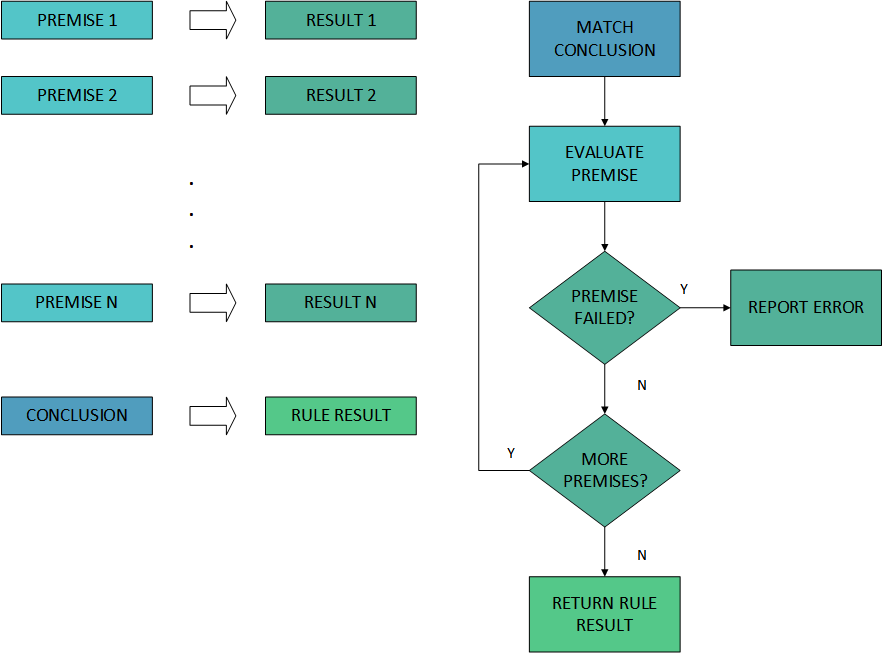
\includegraphics[width = \textwidth]{Figures/chapter_metacasanova/rule_evaluation}
	\caption{Diagram of rule evaluation: on the left side the structure of an inference rule, on the right side its evaluation expressed as a flow chart. The components of the rule are coloured to match the parts in which they are used in the flow chart.}
	\label{fig:ch_metacasanova_rule_evaluation}
\end{figure}

\subsection{Hard-coded implementation of Semantics}
\label{sec:ch_metacasanova_hc_semantics}
As shown in Section \ref{sec:ch_background_semantics}, there are multiple ways to express the semantics of a programming language. In this work we choose to make use of the operational semantics representation to have a uniform way of expressing both the type system and the semantics of a language. Let us consider again the semantics rule for \texttt{if-then-else} and \texttt{while-do} presented in Section \ref{sec:ch_background_semantics}. The operational semantics can be implemented generating the code in the object language that emulates the behaviour of the semantics rule, in the same fashion of a type rule. This process might first pass through an intermediate language, closer to the target language. In the case of an interpreter, the behaviour of the semantics must be implemented using the abstractions available in the host language. As an example, we show a possible implementation of the semantics of the two statements mentioned above in an interpreter both in a functional programming language and in an object-oriented language, as for the type rule.

For convenience, let us make a separate rule for the semantics of a sequence of statements from the specific semantics of the control structure. Also, we introduce the statement \texttt{skip} that performs no operation

\begin{mathpar}
	\mprset{flushleft}
	\inferrule*
	{ }
	{\langle \text{skip} ; ks \rangle \Rightarrow \langle ks \rangle}
\end{mathpar}
\begin{mathpar}
	\mprset{flushleft}
	\inferrule*
	{\langle k \rangle \Rightarrow k'}
	{\langle k ; ks \rangle \Rightarrow \langle k' ; ks \rangle}
\end{mathpar}
\begin{mathpar}
	\mprset{flushleft}
	\inferrule*
	{\langle c \rangle \Rightarrow \text{\texttt{true}}}
	{\langle \text{if \textit{c} then \textit{T} else \textit{E}} \rangle \Rightarrow \text{\textit{T}}}
\end{mathpar}
\begin{mathpar}	
	\mprset{flushleft}
	\inferrule*
	{\langle c \rangle \Rightarrow \text{\texttt{false}}}
	{\langle \text{if \textit{c} then \textit{T} else \textit{E}} \rangle \Rightarrow \text{\textit{E}}}
\end{mathpar}
\begin{mathpar}	
	\mprset{flushleft}
	\inferrule*
	{\langle c \rangle \Rightarrow \text{\texttt{true}}}
	{\langle \text{while \textit{c} do \textit{L}} \rangle \Rightarrow \text{\textit{L} ; while \textit{c} do \textit{L}}}
\end{mathpar}
\begin{mathpar}	
	\mprset{flushleft}
	\inferrule*
	{\langle c \rangle \Rightarrow \text{\texttt{false}}}
	{\langle \text{while \textit{c} do \textit{L}} \rangle \Rightarrow \text{skip} }
\end{mathpar}

As for the type rules, we assume that the data type representing a statement is implemented by a discriminate union. The evaluation function first performs the pattern matching on the argument to select the correct rule to execute, in the same fashion of the type rule, but instead of analysing the types this time executes the specific behaviour of the statement, as specified by the semantics rule. For inference rules above we use the following code:

\begin{lstlisting}
let rec interpretStmt (symbolTable : SymbolTable) (stmt : Statement) : Statement =
  match stmt with
  ... //other statements semantics
  | Sequence(Skip,ks) -> interpretStmt symbolTable ks
  | Sequence(k,ks) ->
  	 let k' = interpretStmt symbolTable k
  	 interpretStmt symbolTable Sequence(k',ks)
  | If (cond,_then,_else) ->
      let condEvaluation = interpretExpr symbolTable cond
      if condEvaluation = True then
      	_then
      else
        _else
  | While (cond,_do) ->
     let condEvaluation = interpretExpr symbolTable cond
     if condEvaluation = true then
       Sequence(_do,While(cond,_do))
      else
        Skip
  ... //other statements semantics
\end{lstlisting}

As for the type evaluation, we assume that \texttt{interpretExpr} is another function that is able to process expressions and return their value. 

The function matches the kind of statement that we want to execute. In the case of a sequence of statements starting with a skip, we simply return the interpretation of the remaining part of the sequence (we indeed skip to the next statement), otherwise we have to run the first statement and then recursively evaluate the sequence formed by the result of the execution of the statement and the rest of the statements. This is needed, for instance, to correctly evaluate the body of a control structure. The body of each match case is responsible of emulating the intended behaviour described in the semantics of the control structure: the \texttt{if} returns the correct block to execute depending on the boolean value of the condition, instead the \texttt{while} returns either its body followed by the same \texttt{while} loop when the condition is \texttt{true}, otherwise \texttt{skip} to jump past the loop.

In the case of an object-oriented language, it is necessary to add a new implementation of the visitor pattern implementing the behaviour of the semantics for each statement:

\begin{lstlisting}
public class StatementInterpreter : StatementVisitor
{
  ... //other statements semantics
  public Statement OnSequence(SymbolTable symbolTable, Sequence seq)
  {
    Statement k = seq.Head;
    Statement ks = seq.Tail;
    if (k.Equals(Skip))
      return ks.Visit(new StatementInterpreter());
    else
    {
      Statement k1 = k.Visit(new StatementInterpreter());
      Statement seq1 = new Sequence(k1,ks)
      return seq1.Visit(new StatementInterpreter());
    }
  }
  public Statement OnIf(Expression cond, Statement _then, Statement _else)
  {
    Value condValue = cond.Visit(new ExpressionInterpreter());
    if (condValue.Equals(new True()))
      return _then;
    else
      return _else;
  }
  public Statement OnWhile(Expression cond, Statement _do)
  {
    Value condValue = cond.Visit(new ExpressionInterpreter());
    if (condValue.Equals(new True()))
      return new Sequence(_do,new While(cond,_do))
    else
      return new Skip();
  }
  ... //other statement semantics
}
\end{lstlisting}

A further remark is that, for the sake of simplicity, here the interpretation only returns a new statement to execute obtained by processing the current statement, but in a real application it should also return a data structure representing the state of the program.

At this point it is possible to observe that this pattern can be generalized as well in a way analogous to that used for type rules for both implementations, which we omit for brevity.


\subsection{Discussion}
In Section \ref{sec:ch_metacasanova_hc_type_rules} and \ref{sec:ch_metacasanova_hc_semantics} we have shown two implementations, one functional and one object-oriented, of type rules and semantics in a possible hard-coded compiler. We have also shown that the pattern can be generalized in both versions. Indeed, their behaviour must be hard-coded in the language chosen for the compiler implementation, regardless of the fact that the pattern is constantly repeated in every rule. This pattern can be captured in a meta-language that is able to process the type system and operational semantics definition of the language and generates the code in the target language necessary to execute the behaviour of the rules. In the following sections we describe the meta-language for \textit{Metacasanova}, a meta-compiler that is able to read a program written in terms of type system/operational semantics rules defining a programming language, a program written in that language, and output executable code that mimics the behaviour of the semantics. The goal of this language is relieving the programmer from writing boiler-plate code when implementing a compiler for a (Domain-Specific) language.

\section{Metacasanova overview}
\label{sec:ch_metacasanova_metacasanova_overview}
In this section we present the general idea behind Metacasanova. We start by defining the requirements of Metacasanova, then we proceed to give a general overview of the language, and finally we formalize the semantics of the language.

\subsection{Requirements of Metacasanova}
In order to relieve programmers of manually defining the behaviour described in Section \ref{sec:ch_metacasanova_hc_type_rules} and \ref{sec:ch_metacasanova_hc_semantics} in the back-end of the compiler, we propose the following features for Metacasanova:

\begin{itemize}
	\item It must be possible to define custom operators (or functions) and data containers. This is needed to define the syntactic structures of the language we are defining.
	\item It must be typed: each syntactic structure can be associated to a specific type in order to be able to detect meaningless terms (such as adding a string to an integer) and notify the error to the user.
	\item It must be possible to have polymorphic syntactical structures. This is useful to define equivalent ``roles'' in the language for the same syntactical structure; for instance we can say that an integer literal is both a \textit{Value} and an \textit{Arithmetic expression}.
	\item It must natively support the evaluation of semantics rules, as those shown above. This will allow the programmer to faithfully implement the formal definition of the language expressed as logical rules. 
\end{itemize}

We can see that these specifications are compatible with the definition of meta-compiler, as the software takes as input a language definition written in the meta-language, a program for that language, and outputs runnable code that mimics the code that a hard-coded compiler would output.

\subsection{Program structure}
\label{subsec:ch_metacasanova_program_structure}
In this section we give an informal idea of how a Metacasanova program is organized. A program in meta-casanova contains the language definition and the rules to evaluate its semantics and/or type system. Further ahead this idea is expanded with additional details when we present the implementation details of the parser.  \\\\
A Metacasanova program is organized in four parts:

\begin{enumerate}
  \item \textit{Includes:} in this part it is possible to include other modules written in Metacasanova and .NET libraries that can be used in the current meta-program.
	\item \textit{Data and function declarations:} in this part it is possible to specify data structures, that define the syntactic constructs of the language, and functions used to evaluate terms of the language through rules.
	\item \textit{Subtype declarations:} in this part it is possible to specify sub-typing by stating that a type $T_1$ is a subtype of another type $T_2$.
	\item \textit{Rule definitions:} in this part the programmer defines the type or semantics rules necessary to describe the type system or behaviour of the abstractions of the programming language.
\end{enumerate}

A data structure or function declaration specifies the types of the arguments to construct the data structure or to pass to the function, their name, and the type of the data structure or the function itself
\begin{lstlisting}
Data Expr -> "+" -> Expr : Expr
\end{lstlisting}

\noindent
Note that Metacasanova allows you to specify any kind of notation for data types in the language syntax, depending on the order of definition of the argument types and the constructor name. In the previous example we used an infix notation. The equivalent prefix and postfix notations would be:

\begin{lstlisting}
Data "+" -> Expr -> Expr : Expr
Data Expr -> Expr -> "+" : Expr
\end{lstlisting}

Optionally, it is possible to specify a precedence priority and the associativity. For example, the following code specifies that the multiplication has a higher precedence over the sum and that both are left-associative.

\begin{lstlisting}
Data Expr -> "+" -> Expr : Expr Priority 0 <|
Data Expr -> "*" -> Expr : Expr Priority 1 <|
\end{lstlisting}

\noindent
A function definition is similar to a data definition but it also has a return type. For instance the following is the evaluation function definition for the arithmetic expression above:

\begin{lstlisting}
Func "eval" -> Expr : Value
\end{lstlisting}

\noindent
Subtyping is defined through the keyword \texttt{is}, which specifies that a type $T_1$ can be used in place of another type $T_2$. For example the following code specifies that a data structure of type \texttt{Value}, such as a list, can be used also as an expression of type \texttt{Expr}.

\begin{lstlisting}
Data "$l" -> List : Value 
Value is Expr
\end{lstlisting}

Metacasanova also allows to embed C\# code into the language by using double angular brackets. This code can be used to embed .NET types when defining data or functions, or to run C\# code in the rules. For example in the following snippet we define a floating point data which encapsulates a floating point number of .NET to be used for arithmetic computations:

\begin{lstlisting}
Data "$f" -> <<float>> : Value
\end{lstlisting}

\noindent
Note that this might be handy for domain-specific languages that need to be used in conjunction with external libraries or frameworks supporting .NET. For example, the domain-specific language Casanova, which we are going to re-implement in Metacasanova in Chapter \ref{ch:languages}, works in conjunction with game engines such as Monogame or Unity.

A rule in Metacasanova may contain a sequence of premises and a conclusion. The rule is executed if the input matches the pattern of the conclusion and all the premises return a result that matches the one specified in their rightmost part. In the following snippet we have the rule to evaluate the sum of two floating point numbers:

\begin{lstlisting}
eval a => $f c
eval b => $f d
<<c + d>> => res
------------------------
eval (a + b) => $f res
\end{lstlisting}

\noindent
Note that if one of the two expressions does not return a floating point value, then the entire rule evaluation fails. Also note that we can embed C\# code to perform the actual arithmetic operation. Metacasanova selects a rule by means of pattern matching (in order of declaration of rules) on the function arguments. This means that both of the following rules will be valid candidates to evaluate the sum of two expressions:

\begin{lstlisting}
...
---------------
eval expr => res

...
----------------
eval (a + b) => res
\end{lstlisting} 

\noindent
A more exhaustive explanation of the syntax of Metacasanova is given in Section \ref{sec:ch_metacasanova_parsing}, while an overview of the general shape of a program can be found in Figure \ref{fig:ch_metacasanova_program_structure}.

\begin{figure}[H]
	\centering
	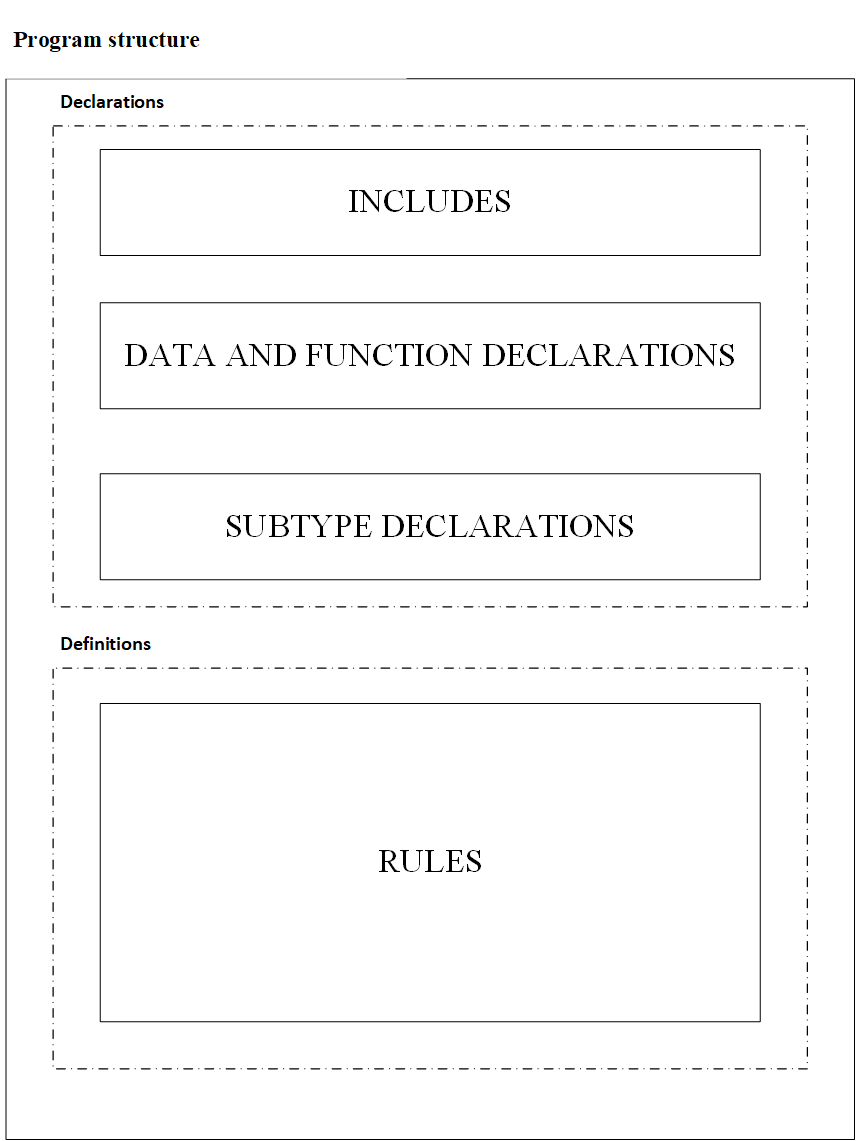
\includegraphics[width = 0.6\textwidth]{Figures/chapter_metacasanova/program_structure}
	\caption{Structure of a program in Metacasanova}
	\label{fig:ch_metacasanova_program_structure}
\end{figure}

\begin{comment}
\subsection{Syntax in BNF}
The following is the syntax of Metacasanova in Backus-Naur form. Note that, for brevity, we omit the definitions of typical syntactical elements of programming languages, such as literals or identifiers:

\begin{lstlisting}[basicstyle = \ttfamily\tiny]
<program> ::= 
{<include>} {<import>} {<data>} <function> {<function>} {<alias>} <rule> {<rule>}
<premise> ::= 
<clause> | <functionCall> | <binding>
<binding> ::= 
id ":=" <constructor>
<rule> ::= 
{premise} "-" {"-"} <functionCall>
<clause> ::= //typical boolean expression
<functionCall> ::= 
<id> {<argument>} <arrow> <argument> | 
{<argument>} <id> {<argument>} <arrow> <argument> | 
<id> {<argument>} <arrow> <argument>
<arrow> ::= "=>" | "==>"
<constructor> ::= 
<id> {<argument>} | 
{<argument>} <id> {<argument>} | 
{<argument>} <id>
<external> ::= "<<" <csharpexpr> ">>"
<csharpexpr> ::= //all available C# expressions
<argument> ::= 
["("] 
(<id> | 
<external> | 
<literal> | 
<constructor>) 
[")"]
<literal> ::= //typical literals such as integer, float, string, ...
<import> ::= import id {"." id}
<include> ::= include id {.id}
<alias> ::= <typeDef> is <typeDef>
<typeDef> ::= id | "<<" id ">>"
<typeArguments> :: = 
'"' <id> '"' {"->" <typeDef>} ":" <typeDef> |
<typeDef> {"->" <typeDef>} "->" '"' <id> '"' {"->" <typeDef>} ":" <typeDef> |
<typeDef> {"->" typeDef} "->" '"' <id> '"' ":" <typeDef> 
<function> ::= Func <typeArguments> "=>" <typeDef> [Priority <literal>]
<data> ::= Data <typeArguments> [Priority <literal>]
\end{lstlisting}
\end{comment}

\subsection{Formalization}
\label{subsec:ch_metacasanova_formalization}
In what follows we assume that the pattern matching of the function arguments in a rule succeeds, otherwise a rule will fail to return a result.
The informal semantics of the rule evaluation in Metacasanova is the following:
\begin{enumerate}[noitemsep]
	\item[R1] A rule with no clauses or function calls always returns a result.
	\item[R2] A rule returns a result if all the clauses evaluate to \texttt{true} and all the function calls in the premise return a result.
	\item[R3] A rule fails if at least one clause evaluates to \texttt{false} or one of the function calls fails (returning no results).
\end{enumerate}
We will express the semantics, as usual, in the form of logical rules, where the conclusion is obtained when all the premises are true.
In what follows we consider a set of rules defined in the Metacasanova language $R$. Each rule has a set of function calls $F$ and a set of clauses (boolean expressions) $C$. We use the notation $f^{r}$ to express the application of the function $f$ through the rule $r$. We will define the semantics by using the notation $\langle expr \rangle$ to mark the evaluation of an expression, for example $\langle f^{r} \rangle$ means evaluating the application of $f$ through $r$. The following is the formal semantics of the rule evaluation in Metacasanova, based on the informal behaviour defined above:


\begin{mathpar}
	\mprset{flushleft}
	\inferrule*[left=R1:]
	{C = \emptyset \\\\ F = \emptyset}
	{\langle f^{r} \rangle \Rightarrow \lbrace x \rbrace} \\
	
	\mprset{flushleft}
	\inferrule*[left=R2:]
	{\forall c_{i} \in C \;, \langle c_{i} \rangle \Rightarrow true \\\\
		\forall f_{j} \in F \; , \exists r_{k} \in R \; | \; \langle f_{j}^{r_{k}} \rangle \Rightarrow \lbrace x_{r^{k}} \rbrace}
	{\langle f^{r} \rangle \Rightarrow \lbrace x_{r} \rbrace} \\
	
	\mprset{flushleft}
	\inferrule*[left=R3(a):]
	{\exists c_{i} \in C \; | \; \langle c_{i} \rangle \Rightarrow false}
	{\langle f^{r} \rangle \Rightarrow \emptyset} \\
	
	\mprset{flushleft}
	\inferrule*[left=R3(b)]
	{\forall r_{k} \in R \; , \exists f_{j} \in F \; | \; \langle f_{j}^{r_{k}} \rangle \Rightarrow \emptyset}
	{\langle f^{r} \rangle \Rightarrow \emptyset}
\end{mathpar}

Note that, in the context of the premise result, we use either a set containing one element or the empty set symbol to denote that the evaluation might succeed and return a result or fail and return no result.
R1 says that, when both $C$ and $F$ are empty (we do not have any clauses or function calls), the rule in Metacasanova returns a result. R2 says that, if all the clauses in $C$ evaluates to true and, for all the function calls in $F$ we can find a rule that returns a result (all the function applications return a result for at least one rule of the program), then the current rule returns a result. R3(a) and R3(b) specify when a rule fails to return a result: this happens when at least one of the clauses in $C$ evaluates to false, or when one of the function applications does not return a result for any of the rules defined in the program.

\section{Architectural overview}
\label{sec:ch_metacasanova_architecture}
In this section we provide a general overview of the architecture of Metacasanova compiler.

The compiler has a modular structure: in the front-end we find the the lexer/parser and a parser post-processing module. The latter is required because not all information necessary to build all the elements of the AST is immediately available during the parsing phase. For instance, some data structures store the file name that is being compiled and the name of the current module, but this information is available only after the parsing itself. 

The generated AST is passed to the type checker to check the type correctness. Note that the type checker of the metacompiler checks the meta-types, i.e. the types defined in the meta-program, and not the types of the terms of the language that is being implemented in Metacasanova. For instance, if one were to re-implement the language C in Metacasanova, the type checker of Metacasanova would be able to type check the elements of the language definition written in Metacasanova (i.e the meta-program), but not a program written in C, which can be checked only by writing a type checker in the meta-program itself. This module checks the correctness of the declarations and the terms used in rules. The type checker outputs a data structure containing information about the types of the declarations and terms used in rules (in short a \textit{typed program definition}).

The output of the AST is passed to the code generator that uses information about the types to correctly generate the target code. This is needed because Metacasanova generates C\# code, which is a typed high-level language that requires information about the types to define variables, methods, and classes representing the elements of the meta-program.

Note that also, with this implementation choice, it is possible to support different high-level programming languages, both typed and untyped: the only component that changes will be the generation of the behaviour of the rules in the abstractions provided by the different target languages. A possible improvement of this architecture is generating a common intermediate language that is later translated into the target code, but this falls outside the scope of this work.


\section{Parsing}
\label{sec:ch_metacasanova_parsing}
In this section we explain in detail the grammar of Metacasanova and we present the architecture of its parser. A full description of the Metacasanova grammar in BNF can be found in Appendix \ref{app:metacasanova_grammar}. The parser has been built in FsYacc (see Section \ref{sec:ch_background_parser_generators}) and completed by a post-processing module that executes some required transformation on the generated AST that are not convenient to perform during the parsing phase. As explained informally in Section \ref{sec:ch_metacasanova_metacasanova_overview}, a Metacasanova program is made of four main sections: (\textit{i}) a part containing inclusion directives, (\textit{ii}) a part containing the declarations of the meta-data stracutures and evaluation functions used in the program, (\textit{iii}) a part containing subtype definitions, and (\textit{iv}) a part containing evaluation rules that define the behaviour of the meta-program. The definition of the first part is trivial, because it is just a sequence of directives starting with the keyword \texttt{include} and followed by a file name. We will instead describe in detail the other parts.
	
\subsection{Declarations}
\label{sec:ch_metacasanova_parser_declarations}
Declarations contain \textit{function} or \textit{data} declarations. A meta-data structure is a meta-language representation of an abstraction of the language implemented in the metacompiler and contains both syntactical and structural information. For example, an arithmetic operator in a programming language can be represented as a meta-data structure containing both its symbol and the values of its arguments. Meta-data structures can be recursive, i.e. it is possible to have arguments that are instances of the same meta-data structure. This is done in order to allow recursive data structures such as lists. A meta-data structure declaration begins with the keyword \texttt{Data} and is followed by a series of arguments, which are separated by arrows, that can be both type names and strings representing the name of the meta-data. It is possible to declare an infix or suffix operator by placing its name after the first position of the arguments. For instance, the following code defines a sum operator for arithmetic expressions with an infix notation.

\begin{lstlisting}
Data Expr -> "+" -> Expr : Expr
\end{lstlisting}

Type names are identifiers that begin with an alphabetic character followed by one or more alphanumeric characters or underscores. The regular expression defining this syntax is expressed as

\begin{lstlisting}
ID ::= ['a'-'z' 'A'-'Z'] ['a'-'z' 'A'-'Z' '_' '0'-'9']+
\end{lstlisting}

Type names can also contain external code enclosed by double angular brackets (\texttt{<<} and \texttt{>>}) to make use of external types such as .NET primitive types (\texttt{int}, \texttt{float}, etc.). The operator names offer a rather high level of customization, since they can be expressed as strings that may contain any symbol usually allowed in strings in programming languages.

The arguments are followed by a type name defining the type of the meta-data structure. Optionally it is possible to specify a priority and the associativity, otherwise the default priority will be -1 and the operator will be left-associative.

Function declarations have the same structure except they begin with the keyword \texttt{Func} instead.

Both data and function declarations may define generic arguments. In order to specify generic arguments, they must be enclosed between square brackets after the declaration keyword. For instance the following code defines a data structure representing a tuple

\begin{lstlisting}
Data[a,b] a -> "," -> b : Tuple[a,b]
\end{lstlisting}

Finally, each declaration must end with a line break. Line breaks are used in Metacasanova to separate different language elements, as in this case.

The grammar production used to describe the syntax of declarations is the following:

\begin{lstlisting}
declaration:
| FUNC genericSeq typeOrNameDeclarations COLON typeDeclaration priority associativity newLineSeq {
Func(processParsedArgs $3 $5 (fst $1) (snd $1) $2 $6 $7) }
| DATA genericSeq typeOrNameDeclarations COLON typeDeclaration priority associativity newLineSeq {
Data(processParsedArgs $3 $5 (fst $1) (snd $1) $2 $6 $7) }
\end{lstlisting}

Since type names and data or function names can appear in any order, the parser generates a support polymorphic data structure in F\#.

\begin{lstlisting}
type TypeDeclOrName =
| Type of TypeDecl
| Name of string
\end{lstlisting}

This data structure is later transformed by the parser post-processor in a \textit{symbol declaration}. A symbol declaration contains all the information about a declaration, including the data or function name, the types of the arguments, the priority, and the generic types. This information is later exploited by the type checker to verify the consistency of the declarations and type check the rest of the program.

\subsubsection{Subtype declarations}
Subtyping has been presented as a separate part of the program but it has a tight relationship with the declarations. A subtype definition has the form

\begin{lstlisting}
T1 is T2
\end{lstlisting}

where T1 and T2 are two meta-type names. They are used to specify that meta-type T1 is a subtype of the meta-type T2 and can replace any argument of type T2 while constructing meta-data structures or calling functions. The grammar rule that defines a subtype declaration is

\begin{lstlisting}
ID IS ID newLineSeq
\end{lstlisting}

\noindent
where \texttt{ID} is the same regular expression used for type names. Again successive subtype declarations should be separated by one or more line breaks. The grammar production generates a list of pairs in the AST containing the types involved in the subtyping. This data structure will be processed at a later stage by the type checker to generate an equivalence table.

\subsection{Rules}
\label{sec:ch_metacasanova_parser_rules}
Rules in Metacasanova are the language elements used to define the behaviour of the meta-program. A rule consists of a set of premises followed by a conclusion. Premises and conclusion are separated by a fraction line. Premises and conclusion are made of a left part consisting of a sequence of arguments, and a right part that can contain either a variable or a sequence of arguments. We call the left part of this syntactical structure the \textit{function call}, while the right part is the \textit{result}. Premises differ from the conclusion as, besides function calls, they can also contain \textit{bindings} and \textit{clauses}. Bindings are simply ways to rename values in the premises in the fashion of bindings in functional languages, while clauses are boolean predicates. Moreover, premises can also contain .NET code to be directly emitted, which can contain any C\# code. The syntax of emitted code is the same as that of a normal premise, except the \textit{function call} is replaced by the code to emit enclosed in double angular brackets. The following is the grammar production defining a premise\footnote{ \texttt{BIND} is the symbol \texttt{:=}}:

\begin{lstlisting}
premise:
| emit premises { $1 :: $2 }
| functionCall premises { $1 :: $2 }
| ID BIND arg newLineSeq premises { (Bind({ Namespace = ""; Name = fst $1 },Position.Create(snd $1,""),$3)) :: $5 }
| arg comparisonOp arg newLineSeq premises { (Conditional($1,$2,$3)) :: $5 }
| { [] }

functionCall:
| argSeq ARROW argSeq newLineSeq { FunctionCall($1,$3) }
\end{lstlisting}

Note that premises are optional (axioms do not have any premise in a logical rule), so an empty list is returned when none is given. Note that the namespace required for variables, such as in the binding, is left empty because at this point the namespace of the program is not available yet. The namespace will be later filled in by the parser post-processor. Also note that, in this stage, we do not check if each function call actually contains a function name, and we simply parse a premise (and a conclusion) as a sequence of arguments, that could be function or data names, variables, literals, or nested expressions. Nested expressions are expressions enclosed in brackets and are themselves sequences of arguments. The actual check that premises and conclusions contain a function name is performed by the type checker, because to correctly identify the function name a complete symbol table, unavailable in this moment, is required. A conclusion has the same syntax as a function call:

\begin{lstlisting}
conclusion:
| argSeq ARROW argSeq newLineSeq { ValueOutput($1,$3) }
\end{lstlisting}

The parser generates a data structure for a rule containing a representation of the premises and the conclusion:

\begin{itemize}[noitemsep]
\item \textit{function call}: A function call is simply a pair of list of arguments, where the left element is the call itself, while the right element is the result.

\item \textit{emit}: Emitted code contains the code in string format and the variable it is assigned to (used to save the result of expressions or function calls).

\item \textit{bind}: Bindings contain the variable name used for the binding and its argument, which can be a literal, the constructor of a meta-data structure, or another variable.

\item \textit{conditional}: Conditionals are boolean expressions that may contain comparison operators. Their representation stores their left and right argument and the comparison operator.
\end{itemize}

\subsection{Parser post-processor}
\label{sec:ch_metacasanova_parser_post-processor}
The parser post-processor is responsible for integrating in the AST all the information that is not directly available during the parsing phase. It is also responsible for re-arranging the terms appearing in the data and function declarations, and those appearing in function calls. Its main functions are the following: (\textit{i}) insert the namespace and file information in the elements of the AST, (\textit{ii}) rearrange the terms parsed from a declaration in a \textit{symbol declaration} data structure, and (\textit{iii}) parenthesize the function call terms according to their priority and associativity and rearrange them in a prefix notation.

The first task is trivial as it requires just to traverse the syntax tree and insert the namespace in all the nodes that should store its value. The process scans the AST starting from the root and recursively adding the namespace and file name into all the nodes that must contain such information until a leaf is reached. Below we explain in detail the other how to accomplish the other two tasks.

\subsubsection{Building the declaration data structure}
As anticipated in Section \ref{sec:ch_metacasanova_parser_declarations}, the name of the data or function and the types of its arguments can appear in any order. For convenience, the AST stores a data structure called \textit{symbol declaration} that separates all the information about a declaration for further use, which is made of the following components:

\begin{itemize}[noitemsep]
	\item The name of the data or function.
	\item The type of the arguments of the data or function.
	\item The return type of the declaration: in the case of a data declaration this defines the type of the meta-data structure itself, while in a function declaration this defines the type of the result returned by the function.
	\item The operator arguments order, which can be prefix, infix, or suffix.
	\item The priority of the operator.
	\item The associativity of the operator.
	\item Possible generic arguments.
	\item The arity (number of arguments) to the left and right of the operator symbol.
\end{itemize}

When the parser processes the arguments of a declaration, it creates a list of terms that can be either a type declaration or a name assigned to the meta-data or function in \texttt{string} format. The different arguments must be recognized and stored appropriately in the symbol declaration. In order to do so, the post-processor scans the arguments. If the argument is a string, then it places it as a first element of a pair, otherwise it places the type declaration in a list of declarations. Algorithm \ref{alg:ch_metacasanova_symbol_args} shows the details of this process. Note that it might be possible that the programmer commits the mistake of defining more than one name for the declaration, since we are still checking the syntax of the program. Thus the algorithm checks that the result of the function does not already contain a declaration name as, if it does, it means that a name argument has already been encountered while scanning the list.

The symbol declaration needs also to store the order of the declaration, its left and right arity, and the type of the declaration. 

For the declaration order we have three options:

\begin{enumerate}[noitemsep]
	\item The first element of the parsed arguments is the declaration name. The declaration is then \textbf{prefix}.
	\item The last element of the parsed arguments is the declaration name. The declaration is \textbf{suffix}.
	\item If both 1 and 2 are false, then the name is in the middle and the declaration is \textbf{infix}.
\end{enumerate}

Finding the left and right arity of an operator can be done simply by splitting the list of arguments in correspondence of the declaration name and then counting the elements of the two lists obtained by the split.

Finally, the post-processor must build the type of the declaration. Types in Metacasanova are represented in a way similar to typed lambda calculus \cite{barendregt2013lambda, church1940formulation}: if a declaration as type arguments $T_{1}, T_{2}, ..., T_{n}$, then its type representation is given as $T_{1} \rightarrow T_{2} \rightarrow ... \rightarrow T_{n}$. This will allow at a later stage the type checking of partial function applications. The post-processor scans the arguments list and recursively adds the element to a data structure representing an \textit{arrow type}. The arrow type contains two elements corresponding to the elements to the left and right of the arrow. It is possible to build a chain of arrow types by recursively adding an arrow type as right argument of another arrow. For instance, to represent the type $A \rightarrow B \rightarrow C$ we use.

\begin{lstlisting}
Arrow(A,Arrow(B,Arrow(C)))
\end{lstlisting}

The algorithm to build the type arrow simply scans the argument list and recursively add the current argument to the left of an arrow type and the result of the recursive call to the remaining part of the list as its right part. This process is shown in Algorithm \ref{alg:ch_metacasanova_symbol_type}. Note that in Metacasanova a declaration might contain no type arguments (only the name), thus we return an empty type as placeholder. If a declaration contains only one type argument then there is no need to build an arrow type and the type argument itself is returned. This is also used as a base case for the recursive build of an arrow type.

\begin{algorithm}
	\caption{Arguments construction in a symbol declaration}
	\label{alg:ch_metacasanova_symbol_args}
	\begin{algorithmic}
		\Function {argSeparation} {$A \text{ list of arguments returned by the parser}$}
			\State $name \gets$ \texttt{""}
			\State $D \gets \emptyset$
			\ForAll {$a \in A$}
				\If {$a \text{ is a string}$}
					\If {$name \neq$ \texttt{""}}
						\AlgError{duplicate function name}
					\Else
						\State $name \gets a$
					\EndIf
				\Else
					\State $D \gets D \cup \lbrace a \rbrace$
				\EndIf
			\EndFor
			\State \Return $(name,D)$
		\EndFunction
	\end{algorithmic}
\end{algorithm}

\begin{algorithm}
	\caption{Type construction in a symbol declaration}
	\label{alg:ch_metacasanova_symbol_type}
	\begin{algorithmic}
		\Function {buildDeclarationType} {$A$ list of arguments returned by the parser}
			\If {$A = \emptyset$}
				\State \Return $Empty$
			\ElsIf {$A = \lbrace x \rbrace$}
				\State \Return $x$
			\Else
				\State $h \gets$ \Call {head} {$A$}
				\State $t \gets$ \Call {tail} {$A$}
				\State $r \gets$ \Call {buildDeclarationType} {$t$}
				\State \Return $h \rightarrow r$
			\EndIf
		\EndFunction
	\end{algorithmic}
\end{algorithm}

\subsubsection{Parenthesization of function calls}
As explained above, Metacasanova allows the declaration of functions and data types expressed with any notation (prefix, suffix, or infix) and with arbitrary associativity and precedence. Furthermore, this is possible regardless of the number of arguments that the data type or the function call uses. Parsing operators according to precedence is a well-known problem that must be solved in order to avoid ambiguity in the language grammar. For instance, the expression \texttt{3 + 5 / 4} can generate two different parse trees: \texttt{(3 + 5) / 4} or \texttt{3 + (5 / 4)}. This ambiguity can be solved by setting the division operator to have a higher precedence over the sum operator, as in traditional arithmetic.

The first attempt to solve this problem was Dijkstra's Shunting-Yard algorithm \cite{dijkstra1961shuntingyard} that takes an expression containing operators and a priority table and returns the same expression in Reverse Polish Notation. This approach was later generalised by operator-precedence parsing which is available in all LALR(1) parser generators. Unfortunately, these approaches deal with binary operators, and are unsuitable for operators of arbitrary arity. Moreover, parse generators such as Yacc allow to define a set of pre-defined language operators but do not allow to specify ``custom'' operators to extend the language with. A notable effort in parsing \textit{mixfix operators} (i.e. operators with an arbitrary position in an expression) using precedence graphs has been done in \cite{danielsson2008parsing}.

In this work we use an AST-transformation technique that changes a function call expressed as a sequence of arguments into a parenthesized version based on defined priorities and associativity. A function call, as defined in Section \ref{sec:ch_metacasanova_parser_rules}, can be the left part of a premise or a conclusion, and is parsed as a sequence of arguments. Each argument can be represented in the following way:

\begin{itemize}[noitemsep]
	\item A literal.
	\item An identifier, that can start with an alphabetic character (\textit{simple id}), or a symbol (such as \texttt{\%, \#, \&, @, ...}) followed by a sequence of alphanumeric characters.
	\item A nested expression, which is any sequence of arguments enclosed between brackets (such as \texttt{(5 + x)}).	
\end{itemize}

We now give the definition of parenthesization of an argument sequence. In what follows we use the term \textit{symbol} to indicate the name of \textit{functions} or \textit{meta-data} structure used in an argument sequence.

\begin{definition}
	\label{def:ch_metacasanova_parenthesization}
	An argument sequence is parenthesized if all its arguments are (\textit{i}) literals, (\textit{ii}) identifiers, or (\textit{iii}) a nested expressions containing a parenthesized argument sequence, and the nesting depth of a symbol is directly proportional to its priority (i.e. the highest-precedence operator is at maximum nesting depth).
\end{definition}

\noindent
For instance, given the precedence relation in Table \ref{tab:ch_metacasanova_example_precedence_relation}, the following argument sequence is parenthesized

\begin{lstlisting}[label = code:ch_metacasanova_par_example,caption = Example of parenthesization]
x -> ($ a1 (b1 % b2 b3) a2)
\end{lstlisting}

\begin{table}
  \centering
	\begin{tabular}{|c|c|c|c|c|}
		\hline
		\textbf{Symbol} & \textbf{Priority} & \textbf{Left arity} & \textbf{Right arity} & \textbf{Associativity} \\
		\hline
		\texttt{\%} & 2 & 1 & 2 & Left \\
		\hline
		\texttt{\$} & 1 & 0 & 3 & Left \\
		\hline
		\texttt{->} & 0 & 1 & 1 & Left \\
		\hline
	\end{tabular}
	\caption{Precedence relation for Listing \ref{code:ch_metacasanova_par_example}}
	\label{tab:ch_metacasanova_example_precedence_relation}
\end{table}

The algorithm takes as input a precedence table with the structure of Table \ref{tab:ch_metacasanova_example_precedence_relation} and the argument sequence to parenthesize, and returns the parenthesized argument sequence. We adopt a recursive approach to the parenthesization problem, whose base case is that the sequence contains only identifiers and literals. Note that a sequence that contains a nested expression is in general not parenthesized because the sequence enclosed in brackets has not been parenthesized yet.

At this point we have two different possibilities for an argument sequence: (\textit{i}) the sequence contains no symbol, or (\textit{ii}) the sequence contains one ore more symbols.

\paragraph{Parenthesization of sequences with no symbols}
When there are no symbols in the sequence of arguments, each argument can be a literal or identifier corresponding to no definition, or a nested expression. In the first case the argument is automatically parenthesized according to Definition \ref{def:ch_metacasanova_parenthesization}. In the second case we must recursively parenthesize the sequence contained in the nested expression. If the result of this parenthesization is a single nested expression, than we take its content and store it into a single nested expression, to avoid redundant nesting parentheses of the form \texttt{((...(a1 a2, ..., an)...))}. If the result is a series of arguments than we just place it inside a nested expression, obtaining something of the form \texttt{(a1 a2 (b1 b2 ...) a3 (c1 c2 ...) ...)}. It might be possible that the recursive algorithm tries to parenthesize a sequence containing no arguments (see the details of the algorithm below). In this case the algorithm simply returns an empty sequence.

\paragraph{Parenthesization of sequences with symbols}
Dealing with sequences containing symbols is more complex, since we must parenthesize them keeping into account the symbols priorities and associativity. According to Definition \ref{def:ch_metacasanova_parenthesization}, in a parenthesized sequence the operator with the lowest priority must be at the top of the sequence nesting. The idea is then that at the current depth we should find the symbol with the lowest priority and a series of parenthesizations containing sequences with symbols of higher priority. The algorithm extracts the symbol in the sequence with the lowest priority and the positions in the sequence where it appears. Note that the same symbol might appear more than once. If the symbol associativity is left then we consider its rightmost occurrence in the sequence, otherwise its leftmost one. Now we split the sequence in two parts using this occurrence as separator and we recursively try to parenthesize these two parts. For instance, let us consider again the Precedence Table \ref{tab:ch_metacasanova_example_precedence_relation} and the following sequence of arguments

\begin{lstlisting}
x -> $ a1 b1 % b2 b3 a2
\end{lstlisting}

\noindent
The algorithm will select the symbol \texttt{->} as a separator, as it is the symbol with the lowest priority (there is only one occurrence, thus we neglect the part that selects the appropriate occurrence). It will then recursively parenthesize the sequences \texttt{x} and \texttt{\$ a1 b1 \% b2 b3 a2}. At this point we have two parenthesizations of the left and right part: $\lbrace l_1, l_2, ..., l_n \rbrace$ and $\lbrace r_1, r_2, ..., r_m \rbrace$ respectively for the left and right sequence. Assuming that the left arity of the current symbol is $a_l$ and the right one is $a_r$, then the parenthesization of the current operator will contain the elements $\lbrace l_{n - a_l + 1}, ..., l_{n} \rbrace$ and $\lbrace r_1, ..., r_{a_r} \rbrace$. Assuming that the current symbol is $\sigma$, we now consider three cases:

\begin{enumerate}
	\item The symbol uses a prefix notation: in this case the parenthesization will not contain any elements from $\lbrace l_{n - a_l + 1}, ..., l_{n} \rbrace$, thus the final parenthesization will be $$\lbrace l_1, l_2, ..., l_n \; (\sigma, r_1, ..., r_{a_r}) \; r_{a_r + 1}, ..., r_{m} \rbrace$$.
	\item The symbol uses an infix notation: in this case the parenthesization will contain elements from both $\lbrace l_{n - a_l + 1}, ..., l_{n} \rbrace$ and $\lbrace r_1, ..., r_{a_r} \rbrace$. The final parenthesization will be $$l_1, ...,l_{n - a_l} \; (l_{n - a_l + 1}, ..., l_{n},\sigma, r_1, ..., r_{a_r}) \; r_{a_r + 1} ,..., r_{m}$$
	\item The symbol uses a suffix notation: in this case the parenthesization will not contain any elements from $\lbrace r_1, ..., r_{a_r} \rbrace$ and the final parenthesization will be $$l_1,...,l_{n - a_l} \; (l_{n - a_l + 1}, ..., l_{n},\sigma) \; r_{1},...,r_{m}$$.
\end{enumerate}

In order to clarify this process, let us consider again the argument sequence

\begin{lstlisting}
x -> $ a1 b1 % b2 b3 a2
\end{lstlisting}

\noindent
and let us apply the algorithm to it (again using the Priority Table \ref{tab:ch_metacasanova_example_precedence_relation}). The algorithm will test the whole sequence looking for symbols, and of course will find one. We then fall in the second part of the algorithm. The symbol with the lowest priority is \texttt{->}, so the algorithm will recursively parenthesize \texttt{x} and \texttt{\$ a1 b1 \% b2 b3 a2}. The left one is a base case of the recursion since the sequence contains only one identifier that is not a symbol, thus its parenthesization is the sequence itself. The right one contains other symbols so we have to recursively apply the algorithm. The operator with the lowest priority is now \texttt{\$}. The symbol is the first element of the sequence, thus the left subsequence obtained by the partitioning phase is empty (and the result of its parenthesization an empty sequence as well). The right subsequence is \texttt{a1 b1 \% b2 b3 a2}. In this sequence there is only one symbol, which is \texttt{\%}, thus the algorithm will try to parenthesize \texttt{a1 b1} and \texttt{b2 b3 a2}. Their parenthesization is trivial and returns the sequences themselves. At this point we have to consider the arity of \texttt{\%}, which accepts one left argument and two right arguments. The algorithm will then enclose between brackets \texttt{b1 \% b2 b3}. The full parenthesization leads then to \texttt{a1 (b1 \% b2 b3) a2}. At this point this result is used to build the parenthesization of \texttt{\$}. This symbol accepts three right arguments (and no left argument), so the parenthesization will be \texttt{(\$ a1 (b1 \% b2 b3) a2) }. Finally we have to use the result to build the parenthesization of \texttt{\%}. This symbol accepts one left argument and one right argument. The parenthesization of its left subsequence was \texttt{x}, while its right parenthesization is \texttt{(\$ a1 (b1 \% b2 b3) a2) }, thus the final parenthesization will be \texttt{(x -> (\$ a1 (b1 \% b2 b3) a2))}. At this point, the outer parenthesization can be removed for better readability.\\
The details of the algorithm are shown in Algorithm \ref{alg:ch_metacasanova_parenthesization}.

\begin{algorithm}
	\small
	\caption{Parenthesization of a sequence of arguments. The operators :: and @ are respectively prepend and append on a list. With the notation $\langle S \rangle$ we denote a sequence $S$ enclosed by parentheses.}
	\label{alg:ch_metacasanova_parenthesization}
	\begin{algorithmic}
		\Function {parenthesize} {$S$ symbols in the sequence, $A$ arguments sequence}
			\If { $A = \emptyset$ }
				\State \Return $A$
			\Else
				\If {$S \neq \emptyset$}
					\AlgLet{$s'$} {the symbol with lowest priority in $S$}
					\AlgLet{$I$} {the set of indices at which $s'$ occurs in $S$.}
					\State $l \gets \emptyset$
					\State $r \gets \emptyset$
					\If {$s'$ is left-associative}
						\State $I' \gets $  \Call {last} {$I$}
						\State $l,r \gets$ \Call {splitAt} {$I'$}
						\State $r \gets$ \Call {tail} {$r$}
					\Else
						\State $I' \gets $  \Call {first} {$I$}
						\State $l,r \gets$ \Call {splitAt} {$I'$}
						\State $r \gets$ \Call {tail} {$r$}
					\EndIf
					\AlgLet{$lsym$}{the symbols in $l$}
					\AlgLet{$rsym$}{the symbols in $r$}
					\State $lpar \gets$ \Call {parenthesize} {$lsym$,$l$}
					\State $rpar \gets$ \Call {parenthesize} {$rsym$,$r$}
					\AlgLet{$larity$}{left arity of $s'$}
					\AlgLet{$rarity$}{right arity of $s'$}
					\State $largs,plargs \gets$ \Call {splitAt} {$|largs| - larity$}
					\State $rargs,prargs \gets$ \Call {splitAt} {$rarity$}
					\If {$larity + rarity > 0$}
						\If {$s'$ is prefix}
							\State $e \gets s' \; :: \; prargs$
						\ElsIf {$s'$ is suffix}
							\State $e \gets plargs \; @ \; s'$
						\Else {$s'$ is infix}
							\State $e \gets plargs \; @ \; s' \; @ \; prargs$
						\EndIf
						\State \Return $largs \; @ \; \langle e \rangle \; @ \; rargs$
					\Else
						\State \Return $largs \; @ \; s' \; @ \; rargs$
					\EndIf
       	\Else
         					\State $p \gets \emptyset$
         					\ForAll {$a \in A$}
         						\If {$a = \langle e \rangle$}
         							\AlgLet{$S'$}{symbols in $e$}
         							\State $p' \gets$ \Call {parenthesize} {$S'$} {$e$}
         							\If {$p' = \langle e' \rangle$}
         								\State $p \gets p \; @ \; e'$
         							\Else
         								\State $p \gets p \; @ \; \langle p' \rangle$
         							\EndIf
         						\Else
         							\State $p \gets p \; @ \; \lbrace a \rbrace$
         						\EndIf
         					\EndFor
         				\EndIf
         			\EndIf		
         		\EndFunction
	\end{algorithmic}
\end{algorithm}

\section{Type checking}
\label{sec:ch_metacasanova_type_checking}
The type checker of Metacasanova is responsible for two tasks: (\textit{i}) checking that the declarations are correctly formed and (\textit{ii}) checking that the premises and conclusions of rules respect the meta-types defined in the declarations. We will now proceed to explain in detail how the two processes are implemented in the metacompiler.

\subsection{Checking declarations}
\label{subsec:ch_metacasanova_checking_declarations}
Checking declarations requires to check the consistency of \textit{meta-type declarations} in each one of the function or data declarations. Note that, from now on, we will refer to meta-types simply as \textit{types} for simplicity. Also we assume that, at this point, we have already built the \textit{symbol table} for the meta-program containing all the symbol declarations with the complete information about the declaration itself. A type declaration in Metacasanova can have five different forms:

\begin{itemize}
	\item \textit{Zero:} A place-holder type used for function or meta-data that do not use any arguments.
	
	\item \textit{External:} Used for embedded types from .NET.
	
	\item \textit{Unsafe:} Unsafe type is a place-holder for external function calls, i.e. function defined in an external embedded language.
	
	\item \textit{Argument:} A type argument is a simple type identifier followed by an optional list of generic arguments used for generic types. For example the type \texttt{Tuple[a,b]} is a type argument whose identifier is \texttt{Tuple} and whose generic arguments are \textit{a} and \textit{b}.
	
	\item \textit{Arrow:} An arrow type has the form \texttt{T1 -> T2 -> ... -> Tn} and is used to represent the type of the arguments used when calling a function or when constructing a meta-data. For example the function declaration \texttt{Func Num -> "+" -> Num : Num} has the \textit{Arrow} type \texttt{Num -> Num}. Note that the symbol declaration, for convenience, stores two different type declarations: the arguments types separated from the function returned type or the meta-data type and a \textit{full type} that combines the type of the arguments and the returned type or data type into a single arrow. For example, for the function above, its full type would be \texttt{Num -> Num -> Num}.
\end{itemize}

The algorithm to check the type declarations behaves differently depending on the form of the type declaration. For \textit{Zero}, \textit{External}, or \textit{Unsafe} type declarations the check always succeeds. For \textit{Arrow} the algorithm recursively checks the left and right part of the arrow. In the case of an \textit{Argument} we have two sub-cases: (\textit{i}) the argument is an identifier with no generic arguments, or (\textit{ii}) the argument is an identifier followed by a number of generic arguments. The first case is simple, as it is enough to check whether the type is defined in the symbol table or not. If the type cannot be found in the symbol table then it is undefined and an error is returned. In the case of a type with generic arguments we must check that the number of provided generics matches the number required for the generic type; then we must check if the provided generic arguments have a correct form. A generic argument can be an identifier or again a type accepting other generic arguments. This is the case, for instance, of a type declaration such as \texttt{Tuple[List[int],Tuple[a,List[float]]]}. In the case of a simple generic identifier we must only check that the generic identifier is in the scope of the declaration. For instance the declaration

\begin{lstlisting}
Func[a,b] "foo" -> a -> b : b
\end{lstlisting}

\noindent
would be a valid declaration since the generic identifiers are in the scope of the declaration, while

\begin{lstlisting}
Func[a,b] "foo" -> a -> b : c
\end{lstlisting}

\noindent
would be invalid if \texttt{c} is not a data type defined in the meta-program. In the case of nested types the algorithm must recursively check again that the type exists and that the generic arguments are valid. The procedure details are described in Algorithm \ref{alg:ch_metacasanova_check_declaration}.

\begin{algorithm}
	\caption{Type checking of a symbol declaration}
	\label{alg:ch_metacasanova_check_declaration}
	\begin{algorithmic}
		\Function {checkDeclaration} {$S$ symbol table, $G$ declared generic arguments, $d$ type declaration}
			\If { $d = \text{\textit{Empty}}$ \textbf{or} $d = \text{\textit{Zero}}$ }
				\State \Return
			\Else
				\State \textbf{let} $G'$ be the generics required for $d$
				\If {$G' \neq \emptyset$} 
					\If {$|G'| \neq |G|$}
						\AlgError{invalid amount of generic arguments}
					\Else
						\ForAll {$g \in G'$}
							\State \Call {checkDeclaration} {$S$,$G$,$g$}
						\EndFor
					\EndIf
				\Else
					\If {$d \in S$ \textbf{or} $d \in G$}
						\State \Return
					\Else
						\AlgError{undefined type}
					\EndIf
				\EndIf
			\EndIf
		\EndFunction
	\end{algorithmic}
\end{algorithm}

\subsection{Checking rules}
Type checking a rule requires type checking its conclusion and all of the premises. In what follows we assume that the parser post-processor has already parenthesized and normalized all the function calls, so that every function call is parenthesized according to symbol priority and associativity and that the symbol name is in the first position of an argument sequence. Moreover, we use the following definition relative to meta-data arguments:

\begin{definition}
	An argument is said to be an \textit{explicit data argument} when it is an expression constructing a meta-data.
\end{definition}

\noindent
For example, in the following meta-program

\begin{lstlisting}[caption = Example of an explicit data argument in Metacasanova,  label = code:ch_metacasanova_explicit_data_argument]
Data Expr -> "+" -> Expr : Expr
Func "eval" -> Expr -> Environment : Value
...

eval a env -> a'
eval b env -> b'
<<a' + b'>> -> v
------------------
eval (a + b) env -> v
\end{lstlisting}

\noindent
the first argument of \texttt{eval} in the conclusion is an explicit data argument. Moreover we use the following definition to define the compatibility of two types.

\begin{definition}
\label{def:ch_metacasanova_type_compatibility}
	Let $T$ be the set of types defined in a meta-program and $E = \lbrace (t_i,t_j) \; | \; t1 \in T \wedge t2 \in T \rbrace$ the set of subtype declarations, then we say that the type $t_1$ is \textit{compatible} with $t_2$ if either $t_1 = t_2$ or $\exists (t_i,t_j) \in E \; | \; t_1 = t_i \wedge t_2 = t_j$.
\end{definition}

\subsubsection{Checking the conclusion}
A conclusion must always contain a function call. In order to type-check the function call correctly, we must check that (\textit{i}) the arity of the function is respected, i.e. that the arguments are not more than what the function expects (the type system of Metacasanova supports partial function application, so it is allowed to pass fewer arguments), and (\textit{ii}) that the type of each argument is compatible with what provided in the declaration. Moreover, since a conclusion might contain explicit data arguments, we have to recursively add all the variables contained in the explicit data arguments to the local variables of the current function, as they could be used in the premises. As an example, refer to Listing \ref{code:ch_metacasanova_explicit_data_argument}, where the variables \texttt{a} and \texttt{b} are defined in the argument of \texttt{eval} and later used in the premises.
Checking the arity of the function is trivial: it is sufficient to compare the length of the given argument sequence with the length of the arguments provided in the declaration. If the length of the argument sequence is greater than the arguments defined in the declaration then an error is returned. Checking type compatibility is more complex and the details are explained below.

The right hand-side of a conclusion might contain a variable or an explicit data argument. In both cases its type checking must be delayed until all premises are processed because a variable appearing in one of them might be used. For example, in Listing \ref{code:ch_metacasanova_explicit_data_argument}, variable \texttt{v} is used in the right hand-side of the conclusion and defined in the result of the last premise.

\subsubsection{Checking a premise}
A premise, as explained in Section \ref{sec:ch_metacasanova_parser_rules}, can be (\textit{i}) a function call, (\textit{ii}) a binding, or (\textit{iii}) a clause.\\\\
In the case of a function call we have to type check the arguments of the function call in the same fashion of the conclusion but with a slight difference: when encountering a variable this must not be added to the local variable set but rather looked up in it. If the lookup fails then the variable is undefined and cannot be used. The same happens when checking the arguments of explicit data arguments. If the call is correctly typed, then we must check its result. The result of a call can be either a variable or an explicit data argument. In the first case the variable is added to the local variables and its type set to the return type of the function. In the case of an explicit data argument then all the arguments that are variable are added to the local variables with the appropriate type read from the meta-data structure declaration and, in case of a nested explicit data argument, the procedure is recursively applied.\\\\
A binding is correctly typed if its right argument is correctly typed. The right argument can be a variable or an explicit data argument so we apply the same method that we used to check variables and explicit data arguments in function calls. If this test succeeds then the left argument of the binding, which is always a variable, is added to the local variables with the type of the right argument.\\\\
A clause is correctly typed if the types of the arguments used in the comparison operator are compatible with respect to the operator itself and if they are themselves correctly typed. For example, for the equality comparison, we must ensure that both arguments are correctly typed. As always, if external types are involved, the test automatically succeeds because nothing can be known at this point about the compatibility of the provided types. Of course the test fails if we use a comparison operator combining external types with types defined in the meta-program, because they will always be incompatible.

\subsubsection{Checking a single argument}
\label{subsec:ch_metacasanova_argument_check}
When checking the type of an argument we have to consider several cases depending on what kind of argument we are inspecting. The reader can find the details of each case below. Note that we will never consider external types as their type checking is delegated to the external code compiler that is used when compiling the generated code, so their type checking in the Metacasanova type checker is always successful.

\paragraph{Checking literals}
If the argument is a literal then we have to consider three sub-cases:

\begin{enumerate}
	\item The expected type is generic. In this case, since we are providing explicitly a literal, the generic can be assigned the specific type of the literal.
	\item The expected type is non-generic. In this case we have to check if the type of the literal is compatible with the expected type. This only happens if the expected type is one of the native types supported by Metacasanova.
	\item The expected type is a meta-data structure requiring generic arguments. In this case the type is always incorrect, since a literal is always incompatible with meta-data.
\end{enumerate}

\paragraph{Checking identifiers}
When we have an identifier as argument, this might be either a symbol for a meta-data structure taking no arguments, or simply a variable. In the first case we simply check that the type of the meta-data structure is compatible with the expected type. In the second case the result depends on whether we are type checking a conclusion or a premise. If we are checking a conclusion, then the variable must be added to the local variables in the scope of the rule, otherwise we must look up the local variables to check if it was previously defined. If the lookup fails then the variable is undefined and an error is returned.

\paragraph{Checking nested expressions}
Checking a nested expression requires, in the first place, to recursively type check the arguments used in the nested expression. If this check succeeds than we must also ensure that the type of the meta-data structure that we are analysing is compatible with the expected type.

\paragraph{Checking the type compatibility}
According to Definition \ref{def:ch_metacasanova_type_compatibility}, a type is compatible with another if they are equal or if, in the symbol table, there exists a specified equivalence between the first type and the second. We have thus to distinguish two cases: (\textit{i}) check if the types are equal and, if this fails, (\textit{ii}) check if the provided type is paired with the expected type in an equivalence table. For the following considerations refer to the type structure defined in Section \ref{subsec:ch_metacasanova_checking_declarations}.

\subparagraph{Testing type equality}
Checking type must consider three options: (\textit{i}) the type is a simple identifier, (\textit{ii}) the type is an Arrow type , and (\textit{iii}) the type is External, Unsafe or Zero.\\\\
In case (\textit{i}) we must compare two Type Arguments $t_1$ and $t_2$ other wise the test fails immediately. In this case it is enough to simply check that $t_1 = t_2$.\\\\
In case (\textit{ii}) we must compare two Arrow types otherwise the test fails immediately. Let us assume that we have $T ::= t_1 \rightarrow t_2 \rightarrow ... \rightarrow t_n$ and $U ::= u_1 \rightarrow u_2 \rightarrow ... \rightarrow u_m$, then we check if $t_1 = t_2$ and recursively apply the type equality test on $t_2 \rightarrow ... \rightarrow t_n$ and $u_m \rightarrow ... \rightarrow u_m$. Note that if $n \neq m$ at some point the test will fail because we will compare a Type Argument with an Arrow Type, which will always fail.\\\\
In case (\textit{iii}) the test succeeds if one of the types (either the provided one or the expected one) is external or unsafe; it also succeeds if both types are Zero types.

\subparagraph{Testing type compatibility}
Compatibility might succeed in only two cases: (\textit{i}) when testing two Argument Types, and when testing two Arrow Types; in all other cases the test fails immediately. In what follows we write $t_1 \equiv t_2$ to say that $t_1$ is compatible with $t_2$.\\\\
In case (\textit{i}) we have to check if the provided type is paired with the expected type in a subtype map stored in the symbol table. If the lookup in the map is unsuccessful then an error is returned.\\\\
In case (\textit{ii}) again we consider $T ::= t_1 \rightarrow t_2 \rightarrow ... \rightarrow t_n$ and $U ::= u_1 \rightarrow u_2 \rightarrow ... \rightarrow u_m$. This time we check if $t_1 \equiv t_2$ and then we recursively check the equivalence of $t_2 \rightarrow ... \rightarrow t_n$ with $u_m \rightarrow ... \rightarrow u_m$. Again, the equivalence test fails if $n \neq m$ because we will end up comparing an Argument Type with an Arrow Type.

\section{Code generation}
\label{sec:ch_metacasanova_code_generation}
Metacasanova uses C\# as target language and generates code compatible with any library compiled in the .NET framework. In this phase we must (\textit{i}) generate the appropriate abstractions in C\# to represent meta-data structures and their subtyping, and (\textit{ii}) generate the code to implement the semantics of the rule evaluation, as described in Section \ref{subsec:ch_metacasanova_formalization}. Note that the modularity of the architecture of the Metacasanova meta-compiler is flexible enough to replace the C\# code generation with another language of choice, provided that the proper code generation functions are re-written for the new target language.

\subsection{Meta-data structures code generation}
The type of each data structure is generated as an interface in C\#. Each data structure defined in Metacasanova is mapped to a \texttt{class} in C\# that implements such interface. The class contains as many fields as the number of arguments the data structure contains. Each field is given an automatic name \texttt{argC} where \texttt{C} is the index of the argument in the data structure definition. The data structure symbols used in the definition might be pre-processed and replaced in order to avoid illegal characters in the C\# class definition. The class contains an additional field that stores the original name of the data structure before the replacement is performed, used for its ``pretty print''. For example the data structure.

\begin{lstlisting}
Data "$i" -> int : Value
\end{lstlisting}

\noindent
will be generated as

\begin{lstlisting}
public interface Value {  }

public class __opDollari : Value
{
	public string __name = "$i";
	public int __arg0;
	
	5
	public override string ToString()
	{
	return "(" + __name + " " + __arg0 + ")";
	}
}
\end{lstlisting}

\subsection{Code generation for rules}
Each rule contains a set of premises that in general call different functions to produce a result, and a conclusion that contains the function evaluated by the current rule and the result it produces. The code generation for the rules follows the steps below:

\begin{enumerate}
	\item Generate a data structure for each function defined in the meta-program.
	\item For each function $f$ extract all the rules whose conclusion contains $f$.
	\item Create a \texttt{switch} statement with a case for each rule that is able to execute the function (the function is in its conclusion).
	\item In the case block of each rule, define the local variables defined in the rule.
	\item Apply pattern matching to the arguments of the function contained in the conclusion of the rule. If it fails, jump immediately to the next case (rule).
	\item Store the values passed to the function call into the appropriate local variables.
	\item Run each premise by instantiating the class for the function used by it and copying the values into the input arguments.
	\item Check if the premise outputs a result and, in the case of an explicit data structure argument, check the pattern matching. If the premise result is empty or the pattern matching fails for all the possible executions of the premise then jump to the next case.
	\item Generate the result for the current rule execution. 
\end{enumerate}

\noindent
In what follows, we use as an example the code generation for the following rule (which computes the sum of two integer expressions in a programming language):

\begin{lstlisting}
eval a -> $i c
eval b -> $i d
<< c + d >> -> e
----------------
eval (a + b) -> $i e
\end{lstlisting}

From now on we will refer to an argument as \textit{explicit data argument} when its structure appears explicitly in the conclusion or in one of the premises, as in the case of \texttt{a + b} in the example above.

\subsubsection{Data structure for the function}
\label{subsubsec:function_generation}

As first step the meta-compiler generates a class for each function defined in the meta-program. This class contains one field for each argument the function accepts. It also contains a field to store the possible result of its evaluation. This field is a \texttt{struct} generated by the meta-compiler defined as follows:

\begin{lstlisting}
public struct __MetaCnvResult<T> { public T Value; public bool HasValue; }
\end{lstlisting}

The result contains a boolean to mark if the rule actually returned a result or failed, and a value which contains the result in case of success.

For example, the function

\begin{lstlisting}
Func eval -> Expr : Value
\end{lstlisting}

\noindent
will be generated as

\begin{lstlisting}
public class eval
{
	public Expr __arg0;
	public __MetaCnvResult<Value> __res;
	...
}
\end{lstlisting}

\subsubsection{Rule execution}

The class defines a method \texttt{Run} that performs the actual code execution. The meta-compiler retrieves all the rules whose conclusion contains a call to the current function, which define all the possible ways the function can be evaluated. It then creates a \texttt{switch} structure where each \texttt{case} represents each rule that might execute that function. The result of the rule is also initialized here (the \texttt{struct} will contain a default value and the boolean flag will be set to \texttt{false}). Each \texttt{case} defines a set of local variables, that are the variables used within the scope of that rule.

\subsubsection{Local variables definitions and pattern matching of the conclusion}

At the beginning of each \texttt{case}, the meta-compiler defines the local variables initialized with their respective default values. It also generates then the code necessary for the pattern-matching of the conclusion arguments. Since variables always pass the pattern-matching, the code is generated only for arguments explicitly defining a data structure (see the examples about arithmetic operators in Section \ref{subsec:ch_metacasanova_program_structure}) and literals. If the pattern matching fails then the execution jumps to the next \texttt{case} (rule). For instance, the code for the following conclusion

\begin{lstlisting}
...
-------------
eval (a + b) -> $i e
\end{lstlisting}

\noindent
is generated as follows

\begin{lstlisting}
case 0:
{
	Expr a = default(Expr);
	Expr b = default(Expr);
	int c = default(int);
	int d = default(int);
	int e = default(int);
	if (!(__arg0 is __opPlus)) goto case 1;
	...
}
\end{lstlisting}

\noindent
Note that an explicit data argument, such in the example above, might contain other nested explicit data arguments, so the pattern-matching is recursively performed on the data structure arguments themselves.

\subsubsection{Copying the input values into the local variables}
When each function is called by a premise, the local values are stored into the class fields of the function defined in Section \ref{subsubsec:function_generation}. These values must be copied to the local variables defined in the \texttt{case} block representing the rule. Particular care must be taken when one argument is an explicit data argument. In that case, we must copy, one by one, the content of the data argument into the local variables bound in the pattern matching. For example, in the rule above, we must separately copy the content of the first and second parameter of the explicit data argument into the local variables \texttt{a} and \texttt{b}. The generated code for this step, applied to the example above, will be:

\begin{lstlisting}
__opPlus __tmp0 = (__opPlus)__arg0;
a = __tmp0.__arg0;
b = __tmp0.__arg1;
\end{lstlisting}

Note that the type conversion from the polymorphic type \texttt{Expr} into \texttt{opPlus} is now safe because we have already checked during the pattern matching that we actually have \texttt{opPlus}.

\subsubsection{Generation of premises}
Before evaluating each premise, we must instantiate the class for the function that they are invoking. The input arguments of the function call must be copied into the fields of the instantiated object. If one of the arguments is an explicit data argument, then it must be instantiated and its arguments should be initialized, and then the whole data argument must be assigned to the respective function field. After this step, it is possible to invoke the \texttt{Run} method of the function to start its execution. The first premise of the example above then becomes (the generation of the second is analogous):

\begin{lstlisting}
eval a -> $i c
\end{lstlisting}

\begin{lstlisting}
eval __tmp1 = new eval();
__tmp1.__arg0 = a;
__tmp1.Run();
\end{lstlisting}

\subsubsection{Checking the premise result}
After the execution of the function called by a premise, we must check if a rule was able to correctly evaluate it. In order to do so, we must check that the result field of the function object contains a value, and if not the rule fails and we jump to the next case (rule), which is performed in the following way:

\begin{lstlisting}
if (!(__tmp1.__res.HasValue)) goto case 1;
\end{lstlisting}

If the premise was successfully evaluated by one rule, then we must check the structure of the result, which leads to the following three situations:
\begin{enumerate}
	\item The result is bound to a variable.
	\item The result is constrained to be a literal.
	\item The result is an explicit data argument.
\end{enumerate}

In the first case, as already explained above, the pattern matching always succeeds, so no check is needed. In the second case, it is enough to check the value of the literal. In the last case, all the arguments of the data argument must be checked to see if they match the expected result. In general this process is recursive, as the arguments could be themselves other explicit data arguments. If the result passes the check, then the result is copied into the local variables, in a fashion similar to the one performed for the function premise. For instance, for the premise

\begin{lstlisting}
eval a -> $i c
\end{lstlisting}

\noindent
the meta-compiler generates the following code to check the result
\begin{lstlisting}
if (!(__tmp1.__res.Value is __opDollari)) goto case 1;
__MetaCnvResult<Value> __tmp2 = __tmp1.__res;
__opDollari __tmp3 = (__opDollari)__tmp2.Value;
c = __tmp3.__arg0;
\end{lstlisting}

\subsubsection{Generation of the result}
When all premises correctly output the expected result, the rule can output the final result. In order to do that, the generated code must copy the right part of the conclusion (the result) into the \texttt{res} variable of the function class. If the right part of the conclusion is, again, an explicit data argument, then the data object must first be instantiated and then copied into the result. For example the result of the rule above is generated as follows:

\begin{lstlisting}
res = c + d;
__opDollari __tmp7 = new __opDollari();
__tmp7.__arg0 = res;
__res.HasValue = true;
__res.Value = __tmp7;
break;
\end{lstlisting}

\noindent
After this step, the rule evaluation successfully returns a result.

This implementation choice is due to the fact that we plan to support partial function applications, thus, when a function is partially applied, there is the need to store the values of the arguments that were partially given. This could still be implemented with static methods and lambdas in C\#, but not all programming languages natively support lambda abstractions, so we chose to have a set-up that allows us to change the target language without dramatically altering the logic of code generation.

\section{Summary}
In this chapter we presented the detailed architecture of the Metacasanova meta-compiler. We started by showing that the process of implementing a compiler exhibits recurring patterns that are always the same independently of the implemented language. We show how to hard-code in different programming languages examples of type and semantics rules for a programming language and then we showed that this process differs only in how we encode these rules int the abstractions of the chosen language, and not in their working logic. Based on these observations, we then defined a list of requirements for Metacasanova. We then proceeded to illustrate the various components of the meta-compiler itself: the parser, the type checker, and the code generator. In the next chapter we will show two examples of languages implemented in Metacasanova: C-{}-, which is a small imperative language, and Casanova, which is a Domain-Specific Language for game development.

		

\chapter{Language Design in Metacasanova}
\label{ch:languages}
\epigraph{A language that doesn't affect the way you think about programming is not worth knowing.}{Alan J. Perlis}
In this chapter we show how to implement languages in Metacasanova. The first language that we implement is a small imperative language called C-{}-. Although tiny, this language contains many common features typical of imperative languages such as control structures, program states, variable scoping, and type annotations. We then proceed to re-implement the semantics of Casanova, a DSL for game development, in Metacasanova, work shown also in \cite{DiGiacomo2017}. Finally, we evaluate the length of the language implementation in Metacasanova against a hard-coded implementation of the same language in a general-purpose programming language, and the runtime performance of programs written in the meta-compiled version against Python.

\section{The C-{}- language}
In this section we present the implementation of a small imperative language called C-{}-. Note that, although the name might suggest this, we do not claim any resemblance with the C programming language, as it lacks several features such as pointer arithmetic, arrays, and functions.

C-{}- allows the use of four built-in values: integer, strings, boolean values, and floating-point numbers in double precision. The language provides three kinds of control structures: if-then-else, while-do, and for loops with the same semantics of usual imperative languages. The language supports variable scoping and shadowing

The memory is represented using a dictionary that pairs variable names with their value. In what follows we omit the details of the lookup of entries in the dictionary for brevity. Suffice to say that the meta-program makes use of the \texttt{ImmutableDictionary} data structure available in .NET. Also note that C-{}- defines scopes for variables, so that if a variable is declared inside the scope of a code block in a control structure, that is usable only within the scope itself.

The core of the meta-program is made of the evaluation of both expressions and statements. We proceed below to present the details of both kinds of evaluation.

\subsection{Expression Semantics}
\label{subsec:ch_mcnv_languages_expression_semantics}
As explained above C-{}- supports boolean, string, integer, and floating-point values. These are represented through the following meta-data structures in the meta-program.

\begin{lstlisting}
Data "$i" -> <<int>> : Value Priority 300
Data "$d" -> <<double>> : Value Priority 300
Data "$s" -> <<string>> : Value Priority 300
Data "$b" -> <<bool>> : Value Priority 300
\end{lstlisting}

\noindent
Note that we are using the .NET data types to represent the actual values stored in the meta-data structures. We also define the following type equivalence, since values are atomic cases of expressions and can be used as such:

\begin{lstlisting}
Value is Expr
\end{lstlisting}

\noindent
Expressions can also contain variables, thus we need a meta-data structure to represent them as well.

\begin{lstlisting}
Data "$" -> <<string>> : Id Priority 300
\end{lstlisting}

\noindent
Variables can be used as atomic expressions as well, so we need an additional type equivalence

\begin{lstlisting}
Id is Expr
\end{lstlisting}

\noindent
We now define a data structure to represent the state of the program. The state is simply a map where the key is a variable name and the stored element a valid value in C-{}-. In the declaration we will define the meta-type \texttt{SymbolTable}, and from now on we will refer use the term ``symbol table'' as a synonym of ``state''.

\begin{lstlisting}
Data "$m" << ImmutableDictionary<Id, Value> >> : SymbolTable 
\end{lstlisting}

\noindent
Since we want to allow variable scoping, the state of the program is not represented by a single map, but by a list of maps. Each time the program enters a different scope context, an empty map is added to this list, and removed when the program exits the scope. This process will be further explained below. We define a meta-data structure to represent this list of states (note that the operator for the construction of the list is infix).

\begin{lstlisting}
Data SymbolTable -> "::" -> TableList : TableList
Data "[]" -> TableList
\end{lstlisting}

\noindent
We can finally proceed to define a meta-data structure to represent the operations for expressions. First we define the arithmetic operators in the language:

\begin{lstlisting}
Data Expr -> "+" -> Expr : Expr
Data Expr -> "-" -> Expr : Expr
Data Expr -> "*" -> Expr : Expr
Data Expr -> "/" -> Expr : Expr
\end{lstlisting}

\noindent
then we can define operators for boolean expressions:
\begin{lstlisting}
Data Expr -> "&&" -> Expr : Expr
Data Expr -> "||" -> Expr : Expr
Data "!" -> Expr : Expr
\end{lstlisting}

\noindent
and finally comparison operators:
\begin{lstlisting}
Data Expr -> "equals" -> Expr : Expr
Data Expr -> "neq" -> Expr: Expr
Data Expr -> "ls" -> Expr : Expr
Data Expr -> "leq" -> Expr : Expr
Data Expr -> "grt" -> Expr : Expr
Data Expr -> "geq" -> Expr : Expr
\end{lstlisting}

We now have to define the function that evaluates an expression through rules in the program. This function takes as input the list of symbol tables (needed to read possible variables), an expression, and returns the value after computing the expression.

\begin{lstlisting}
Func "evalExpr" -> TableList -> Expr : Value
\end{lstlisting}

\noindent
Now we have to proceed to define the rules to compute the actual evaluation of an expression. Clearly the base cases of the evaluation are the atomic values, where we immediately return the value itself.

\begin{lstlisting}
-----------------------------
evalExpr tables ($i v) -> ($i v)

-----------------------------
evalExpr tables ($d v) -> ($d v)

-----------------------------
evalExpr tables ($s v) -> ($s v)

-----------------------------
evalExpr tables ($b v) -> ($b v)
\end{lstlisting}

Evaluating variables is more complex: we have to look at the table currently in the head of the list of tables (which is the one relative to the current scope). If we do not find the required variable we have to recursively look it up in the tail of the list, since we could have an arbitrary amount of nested scopes. When the variable is found we return its value. This behaviour is implemented by the following code:

\begin{lstlisting}
symbols contains ($name) -> Yes
symbols lookup ($name) -> val
-------------------------------------------
evalExpr (symbols :: tables) ($name) -> val

symbols contains ($name) -> No
evalExpr tables ($name) -> val
-------------------------------------------
evalExpr (symbols :: tables) ($name) -> val

\end{lstlisting}

We proceed now to define the evaluation of arithmetic operators. We show only the example of the sum for brevity, the other rules differ only in the operator. Evaluating the arithmetic expression requires to recursively call \texttt{evalExpr} on the right and left argument. These recursive calls will eventually return two values that are the result of the two evaluations. After we obtain these values, we can compute their sum and return it as result.

\begin{lstlisting}
evalExpr tables expr1 -> ($i val1)
evalExpr tables expr2 -> ($i val2)
<<val1 + val2>> -> v
---------------------------------------
evalExpr tables expr1 + expr2 -> ($i v)
\end{lstlisting}

\noindent
Note that we have used .NET external code in the third premise to compute the result of the arithmetic operation. Evaluating arithmetic operations involving floating-point expressions can be done in an analogous way, except in the premises we expect to have the meta-data structure for floating-point values as result of \texttt{evalExpr}:

\begin{lstlisting}
evalExpr tables expr1 -> ($d val1)
evalExpr tables expr2 -> ($d val2)
<<val1 + val2>> -> v
---------------------------------------
evalExpr tables expr1 + expr2 -> ($d v)
\end{lstlisting}

\noindent
The same can be said for the string concatenation.
The evaluation of boolean expression is analogous: we show again only the evaluation for AND as the other rules are analogous:

\begin{lstlisting}
evalExpr tables expr1 -> ($b val1)
evalExpr tables expr2 -> ($b val2)
<<val1 && val2>> -> b
----------------------------------------------------------------------
evalExpr tables expr1 && expr2 -> b
\end{lstlisting}

\noindent
Again we rely on external code to compute the actual boolean value.
As for the comparison operators, we can use a clause in the premise to avoid using external code in the following way:

\begin{lstlisting}
evalEpxr tables expr1 -> val1
evalExpr tables expr2 -> val2
val1 == val2
------------------------------------------------
evalExpr tables (expr1 equals expr2) -> $b true

evalEpxr tables expr1 -> val1
evalExpr tables expr2 -> val2
val1 != val2
------------------------------------------------
evalExpr tables (expr1 equals expr2) -> $b false
\end{lstlisting}

\noindent
The first rule checks that the values computed by evaluating the left and right argument of the equality comparison are the same. If this happens then the rule returns a meta-data structure containing the boolean representation of \texttt{true}. Otherwise the first rule fails and the second one is executed. This one will return a boolean representation of \texttt{false} when the values are different.

For inequality operators we must rely on external code for the computation is Metacasanova only allows equality comparisons in clauses:

\begin{lstlisting}
evalExpr tables expr1 -> ($i val1)
evalExpr tables expr2 -> ($i val2)
<< val1 < val2 >> -> boolResult
---------------------------------------------------------
evalExpr tables (expr1 ls expr2) -> ($b boolResult)
\end{lstlisting}

\noindent
The evaluation of the other comparison operators is implemented through analogous rules, which differ only in the operators.

\subsection{Statement Semantics}
\label{subsec:ch_mcnv_languages_statement_semantics}

Statement evaluation requires the definition of a different function, \texttt{eval}, that processes each statement and returns the result of the statement evaluation and the updated state. Note that, even if the evaluation of statements does not always change the state, in general we have to assume that this will happen.

The function \texttt{eval} takes as input a statement to process and the current state (list of symbol tables), and returns the updated list of symbol tables

\begin{lstlisting}
Func "eval" -> TableList -> Stmt : TableList
\end{lstlisting}

We now proceed to define the meta-data structures necessary to represent the statements of the language: C-{}- supports (\textit{i}) variable declarations, (\textit{ii}) variable assignment, (\textit{iii}) if-then-else, (\textit{iv}) while loops, and (\textit{v}) for loops.

Variable declarations follow the same structure of standard C, that is a type name followed by an identifier. Thus, the corresponding meta-data structure can be defined as:

\begin{lstlisting}
"variable" -> Type -> Id : Stmt
\end{lstlisting}

\noindent
Analogously, variable assignment follows the C convention and uses the \texttt{=} symbol.

\begin{lstlisting}
Id -> "=" -> Expr : Stmt
\end{lstlisting}

The control structure if-then-else does not follow the standard C representation, rather we use the keywords \texttt{then} and \texttt{else} to delimit its code blocks. Note that nothing would prevent to implement the conventional C syntax, but we prefer this ``lightweight'' representation. The keywords \texttt{then} and \texttt{else} are meta-data structures that take no arguments and do not have any functional utility other than syntactical mark-ups.

\begin{lstlisting}
Data "then" : Then
Data "else" : Else
Data "if" -> Expr -> Then -> Stmt -> Else -> Stmt : Stmt
\end{lstlisting}

Analogously we can define the meta-data structure for \texttt{While} and \texttt{For}

\begin{lstlisting}
Data "do" : Do
Data "while" -> Expr -> Do -> Stmt : Stmt
Data "for" -> Expr -> Expr -> Epxr -> Do -> Stmt : Stmt
\end{lstlisting}

\noindent
Up to this point we are able to define single statements in the language, but we need a way to concatenate a sequence of statements to form code blocks, in the fashion of C. This is done by introducing an additional meta-data structure, which is the ";" symbol. For convenience, we also introduce a \texttt{nop} statement, which does not do anything, but it will be useful to express the semantics of statements evaluation.

\begin{lstlisting}
Data Stmt -> ";" -> StmtList : StmtList
Data "nop" -> :Stmt

StmtList is Stmt

\end{lstlisting}

We now proceed to define the semantics of statement evaluation.

\subsubsection{Evaluating a Sequence of Statements}
The evaluation of a sequence of statements require to evaluate the first statement in a sequence and then recursively evaluate the rest of the sequence. The recursive evaluation returns the final program state. The base case of the recursion is met when the sequence contains only \texttt{nop}. In this case we terminate the evaluation and return the unchanged program state.

\begin{lstlisting}
--------------------------
eval tables nop -> tables

eval tables a -> tables'
eval table' b -> res
---------------------------
eval tables (a;b) -> res
\end{lstlisting}

\subsubsection{Variable Declarations and Assignments}
Evaluating a variable declaration simply adds the variable to the symbol table of the current scope. Note that we allow variable shadowing, so it is possible to redefine the same symbol in different scopes.

\begin{lstlisting}
symbols defineVariable id -> symbols'
-------------------------------------
eval (symbols nextTable tables) (variable t id) -> symbols' nextTable tables
\end{lstlisting}

\noindent
This rule is executed whenever the processed statement matches the structure of a variable declaration statement. The premise adds the symbol to the symbol table of the current scope (we omit the details for brevity), and returns an updated symbol table. The list of symbol 
tables is rebuilt to include the updated table and returned as result.

Variable assignment is more complex, since the variable we are trying to use might not be in the symbol table of the current scope. We must then define two lookups functions, that behave differently depending on whether the variable is in the symbol table in the head of the symbol table list or not. We declare the function \texttt{updateTable} that performs this lookup and updates the table list accordingly. 

\begin{lstlisting}
Func "updateTables" -> TableList -> TableList -> Id -> Expr : EvaluationResult
\end{lstlisting}

\noindent
In the case that the variable is in the symbol table in the head of the list of tables we have the following rule:

\begin{lstlisting}
symbols contains id -> Yes
evalExpr vars expr -> val
symbols add id val -> symbols'
-------------------------------
updateTables vars (symbols :: tables) id expr -> symbols' :: tables
\end{lstlisting}

\noindent
The first premise checks if the symbol is contained in the table in the head of the list. If the answer is \texttt{Yes} (a meta-data structure returned by the function \texttt{contains}, not described here again for brevity), then the second premise proceeds to evaluate the expression in the right hand-side of the assignment. The third premise adds the value obtained as result of the second premise to the current symbol table and returns the modified table. The new table is then placed in the head of the table list and the whole list is returned. Note that, at this point, all the tables in the list remain unchanged except the one that was in the head. Note that \texttt{updateTables} carries two copies of the list of tables. One of them is passed to \texttt{eval} because the right-hand side of the assignment might contain other variables. The process of looking up the left hand-side variable pops symbol tables from the head of list (see next rule) but the original list of tables is necessary when assigning the values of variables located in inner scopes. For instance, consider the following program in C-{}-:

\begin{lstlisting}[caption = C-{}- sample program, label = code:ch_mcnv_languages_c--_sample_program]
int x;
...
if (x > 0) then
	int y;
	y = 4
	x = y;
else
  x = x - 1;	
\end{lstlisting}

\noindent
assume that before the if-then-else $x > 0$. The program will enter the \texttt{then} block and declare \texttt{y}. In the current state we have to symbol tables, one for the scope of the \texttt{if-then-else} and one for the outer scope. When assigning \texttt{y} to \texttt{x} the symbol table tries to look up \texttt{x} in the table of the current scope and fails. This will pop the head of the list of tables (which is the table of \texttt{if-then-else}) and recursively look in the tail. During the second attempt \texttt{x} is retrieved but now we do not have the symbol table where \texttt{y} is defined anymore to evaluate the right hand-side. We thus need the original list of tables to be able to retrieve \texttt{y}. In general, if we call \texttt{$d_l$} the depth of scoping of the left hand-side and $d_r$ the depth of scoping of the right hand-side, the process pops the table of the right hand-side whenever $d_l > d_r$ and this is when we need the original list of tables to retrieve the value of the right hand-side.

If the variable is not contained in the head of the list, i.e. it has not been declared in the current scope, we have the following rule:

\begin{lstlisting}
symbols contains id -> No
updateTables vars tables id expr -> tables'
----------------------------------------------
updateTables vars (symbols :: tables) id expr -> symbols :: tables'
\end{lstlisting}

The first premise tries to lookup the variable in the symbol table of the current scope and does not find it. Thus we recursively call \texttt{updateTables} with the tail of the list. The recursive call will eventually find the variable in one of the symbol tables associated with outer scopes. This process will produce an updated list of tables that is returned as a new tail for the current list.

At this point, the rule for the evaluation of the variable assignment simply class the \texttt{updateTables} function in its premise:

\begin{lstlisting}
updateTables tables tables id expr -> res
----------------------------------------
eval tables (id = expr) -> res
\end{lstlisting}

\subsubsection{Conditionals}

Evaluating \texttt{if-then-else} requires two rules, depending on the result of the evaluation of its condition. The following rule implements the semantics when the condition is false:

\begin{lstlisting}
evalExpr tables condition -> $b true
emptyDictionary -> table
eval (table :: tables) thenBlock -> table' :: tables''
-------------------------------------------------------------------
eval tables (if condition then thenBlock else elseBlock) -> tables''
\end{lstlisting}

The first premise evaluates the condition of the control structures and succeeds if the result is a meta-data structure containing the boolean value \texttt{true}. The second premise uses an utility function to initialize an empty symbol table. This is required to define a new table for the scope of the conditional. The third premise evaluates the statements contained in the then block after pushing the symbol table for the current scope in the list of symbol tables. This process will eventually produce a new list of symbol tables. The result returns only the tail of this list, since when we exit the scope of the conditional we must pop its symbol tables.

For instance, consider again the program in Listing \ref{code:ch_mcnv_languages_c--_sample_program} and again assume that $x > 0$. After executing the then block, the state of the program is made of the symbol tables shown in Table \ref{tab:ch_mcnv_languages_tables_ifthenelse}. After exiting the then block, variable \texttt{y} exits the scope, thus we have to pop the symbol table for the current scope. However, the symbol table of the outer scope has been changed because \texttt{x} got the value of \texttt{y}. Thus the evaluation returns the list containing this updated table. In general, the process should consider that an arbitrary number of symbol tables for each outer scope has been changed, thus we return this updated list.

\begin{table}
	\centering
	\begin{tabular}{|l|l|}
		\hline
		\textbf{Variable} & \textbf{Value} \\
		\hline
		x & undefined\\
		\hline
	\end{tabular}\\
	\vspace{0.2cm}
	\begin{tabular}{|l|l|}
		\hline
		\textbf{Variable} & \textbf{Value} \\
		\hline
		y & 4\\
		\hline
	\end{tabular}
	\begin{tabular}{|l|l|}
		\hline
		\textbf{Variable} & \textbf{Value} \\
		\hline
		x & 4\\
		\hline
	\end{tabular}
	\caption{Symbol table at the beginning and after the execution of the program in Listing \ref{code:ch_mcnv_languages_c--_sample_program} with $x > 0$}
	\label{tab:ch_mcnv_languages_tables_ifthenelse}
\end{table}

The rule that evaluates conditionals when the condition is false is analogous, except this time we evaluate the else block:

\begin{lstlisting}
evalExpr tables condition -> $b false
emptyDictionary -> table
eval (table :: tables) elseBlock -> table' :: tables''
--------------------------------------------------------------------
eval tables (if condition then thenBlock else elseBlock) -> tables''
\end{lstlisting}

\subsubsection{While Loops}
\label{subsec:ch_mcnv_languages_cmm_loops}
Evaluating the while loops require to check its condition first. When the condition is false we simply skip the loop without changing the state. The rule to implement this behaviour is thus straightforward:

\begin{lstlisting}
evalExpr tables condition -> $b false
--------------------------------------------
eval tables (while condition do block) -> tables
\end{lstlisting}

\noindent
The semantics when the condition is true is more complex:

\begin{lstlisting}
evalExpr tables condition -> $b true
emptyDictionary -> table
eval (table :: tables) block -> table' :: tables''
eval tables'' (while condition do block) -> res
---------------------------------------------------
eval tables (while condition do block) -> res
\end{lstlisting}

\noindent
The first premise succeeds when the evaluation of the condition returns a true boolean value in C-{}-. Analogously to what we did for conditionals, we initialize an empty symbol table for the current scope and we push it into the list of symbol tables. We then evaluate the body of the loop. This process will, in general, produce an updated list of symbol tables. Again we pop the symbol table for the current scope because we are exiting the loop. We then evaluate again the whole loop to test its condition again.

\subsubsection{For Loops}
For loops follow the C convention and are made of four parts: (\textit{i}) an initialization, (\textit{ii}) a condition (\textit{ii}), (\textit{iii}) a step, and (\textit{iv}) a block of code. The initialization is evaluated once before entering the loop, the condition is tested before each iteration of the loop, and the step is evaluated at the end of each iteration. In order to implement this behaviour we make use of an additional support function called \texttt{loopFor}:

\begin{lstlisting}
Func "loopFor" -> TableList -> Expr -> Stmt -> Stmt : TableList
\end{lstlisting}

\noindent
The evaluation of the \texttt{for-loop} evaluates the initialization in its premise. It then calls \texttt{loopFor} after the initialization has been evaluated. Again the initialization might define additional variables that enter the scope of the loop, so the updated table of the current scope is pushed into the list of symbol tables. Note that possible variables defined in the initialization part of the loop might be used after the loop itself, according to the semantics of C, so we have to insert them into the symbol table of the current scope and not the one of the loop itself.

\begin{lstlisting}
eval tables init => tables'
loopFor tables' condition step block => res
-------------------------------------------------------
eval tables (for init condition step do block) => res
\end{lstlisting}

The rules for \texttt{loopFor} are two, since we must consider the case when the condition is false and the one where it is true. When the condition is false the loop is completely skipped, thus we simply return the current state without any changes, in the same fashion of the \texttt{while-loop}:

\begin{lstlisting}
evalExpr tables condition -> $b false
--------------------------------------
loopFor tables condition step block -> tables
\end{lstlisting}

\noindent
When the condition is true, we create as usual a symbol table for the scope of the loop and we push it into the list of symbol tables. The third premise evaluates the block of the loop returning an updated list of tables. As usual we pop the table of the scope of the loop and we evaluate the step. This again might change the list of symbol tables. We then run again the loop with the updated list of tables.

\begin{lstlisting}
evalExpr tables condition -> $b true
emptyDictionary -> table
eval (table :: tables) block -> table' :: tables''
eval tables'' step -> tables3
loopFor tables3 condition step expr -> res 
-------------------------------------------------
loopFor tables condition step block -> res
\end{lstlisting}

\subsection{Type Checker}
\label{subsec:ch_mcnv_languages_type_checking}
Type checking can be performed by using a representation of the type system of C-{}- in terms of rules, in the same fashion of the semantics. In this section we explain the details of how each language construct is type-checked according to its type rule. We begin by defining an alternative version of the symbol table defined in Section \ref{subsec:ch_mcnv_languages_expression_semantics} that contains a mapping between variable names and types:

\begin{lstlisting}
Data "$m" << ImmutableDictionary<Id, Type> >> : TypeTable 
\end{lstlisting}

\noindent
and a constructor for the meta-data representing a sequence of type tables.

\begin{lstlisting}
Data TypeTable -> "::" -> TypeTableList : TypeTableList
Data "[]" : TypeTable
\end{lstlisting}

\noindent
We now start by defining the meta-data structures for the types in C-{}-:

\begin{lstlisting}
Data "t_int" : Type
Data "t_double" : Type
Data "t_string" : Type
Data "t_bool" : Type
Data "t_unit" : Type
\end{lstlisting}

\noindent
We also defined a special meta-data representing a type error to correctly report errors if the program contains invalid types:

\begin{lstlisting}
Data "error" -> <<string>> : Type
\end{lstlisting}

\subsubsection{Typing expressions}

We now proceed to define the type rules for expressions. We initially need to define a function to use in the conclusion of a type rule that is able to evaluate type of an expression:

\begin{lstlisting}
Func "typeExpr" -> TypeTableList -> Expr : Type
\end{lstlisting}

The axioms of expression typing are those that return the type of a literal. In this case the rule immediately returns the type associated to the specific literal.

\begin{lstlisting}
-----------------------------
typeExpr tables ($i v) -> t_int

-----------------------------
typeExpr tables ($d v) -> t_double

-----------------------------
typeExpr tables ($s v) -> t_string

-----------------------------
typeExpr tables ($b v) -> t_bool
\end{lstlisting}

\noindent
Type checking variables require to perform a lookup for the variable name in the list of type tables that we carry along during the typing process. The variable could be in the table associated with the current scope or in the table of an outer scope. Therefore, we start by first looking in the table of the current scope, and if we do not find the variable we recursively look it up in the subsequent table. If we traverse the whole list of tables without finding the variable, then it means that the program contains an undefined variable and an appropriate error notifying the problem should be returned.

\begin{lstlisting}
-------------------------------------
typeExpr [] ($ name) -> error <<"Undefined variable:" + name>>

types contains ($ name) -> Yes
types lookup ($ name) -> varType
------------------------------------------------
typeExpr (types :: tables) ($ name) -> varType

types contains ($ name) -> No
typeExpr tables ($ name) -> error msg
------------------------------------------
typeExpr (types :: tables) ($ name) -> error msg 

types contains ($ name) -> No
typeExpr tables ($ name) -> varType
------------------------------------------
typeExpr (types :: tables) ($ name) -> varType 
\end{lstlisting}

Note that we had to include a rule in whose premise we check whether the recursive lookup returned an error. If this is the case the entire rule returns the error message rather than the type of the variable.

Type-checking expression operators require to perform the following steps:

\begin{enumerate}[noitemsep]
	\item Type-check the left and right argument.
	\item Check that the types obtained at the previous step are compatible with the operator definition.
	\item Return the type of the operator.
\end{enumerate}

\noindent
The process fails when the type-checking of one of the two expressions fails or when the types are incompatible with the operator definition. For brevity we only present the case of the sum, the rules for the other operators are analogous:

\begin{lstlisting}
typeExpr tables expr1 -> error msg
----------------------------------
typeExpr tables expr1 + expr2 -> error msg

typeExpr tables expr2 -> error msg
----------------------------------
typeExpr tables expr1 + expr2 -> error msg

typeExpr tables expr1 -> t_int
typeExpr tables expr2 -> t_int
--------------------------------------
typeExpr tables expr1 + expr2 -> t_int

typeExpr tables expr1 -> t_double
typeExpr tables expr2 -> t_double
--------------------------------------
typeExpr tables expr1 + expr2 -> t_double

typeExpr tables expr1 -> t_string
typeExpr tables expr2 -> t_string
--------------------------------------
typeExpr tables expr1 + expr2 -> t_string

-----------------------------------
typeExpr tables expr -> 
  error << "Incompatible types given to operator +" >>
\end{lstlisting}

\noindent
Note that the last rule is executed only if all the previous failed, so when the recursive check did not fail or when the returned types were incompatible with the sum operator.

\subsubsection{Typing a sequence of statements}
Typing a sequence of statements requires to type check the first statement in the sequence and then recursively type check the remaining statements in the sequence. We also need a different type-checking function that is able to process statements and meta-data structure for its result.

\begin{lstlisting}
Data TypeTableList -> "," -> Type : TypeResult
Func "typeStmt" -> TypeTableList -> Stmt : TypeResult
\end{lstlisting}

\noindent
This function in general returns an updated list of type tables and a type, since variable declarations might change them. We use \texttt{t\textunderscore unit} for the type of statements, which is a place holder for language constructs that just change the state of the program.

The base case of the recursion is when the sequence contains only \texttt{nop}, which returns immediately the same type tables.

\begin{lstlisting}
------------------------------------
typeStmt tables nop -> tables,t_unit
\end{lstlisting}

\noindent
Type-checking a sequence of statements initially checks the first statement. This might return an updated list of tables. Then it recursively checks the other statements with the result of the first step and returns the final type tables. If either of the process returns an error we just propagate the error.

\begin{lstlisting}
typeStmt tables a -> tables',error msg
------------------------------------------
typeStmt tables (a;b) -> tables',error msg

typeStmt tables a -> tables',t_unit
typeStmt tables' b -> finalTables,error msg
----------------------------------------------
typeStmt tables (a;b) -> finalTables,error msg


typeStmt tables a -> tables'
typeStmt tables b -> finalTables,t_unit
--------------------------------
typeStmt tables (a;b) -> finalTables,t_unit
\end{lstlisting}

\noindent
Note that we are sure that the final rule succeeds because the type-checking of a statement always returns \texttt{unit} if the type-checking succeeds, according to the type rules of the language; this is further explained in the sections below.

\subsubsection{Typing variable declarations and assignments}
When we encounter a variable declaration we have to add the variable name and its type to the table of the current scope, unless the variable is already defined in the current scope, in which case we return an error. We must also prevent the declaration of variable with type \texttt{unit}, because that is a reserved type for statements. This is implemented with the following rules:

\begin{lstlisting}

-----------------------------------
typeStmt types (variable t_unit id) -> [],error << "The type unit cannot be used as a variable type" >>

types contains id -> Yes
------------------------------------
typeStmt (types :: tables) (variable t ($ name)) -> [],error << "Variable " + name " already defined" >>

types add id t -> types'
------------------------------------------
typeStmt (types :: tables) (variable t id) -> types' :: tables
\end{lstlisting}

In the case of a variable assignment, the type checker must first look up in the type tables for the variable type. If the variable cannot be found then an error is returned because the program is trying to use an undefined variable. Otherwise we check the type of the right expression, and if it is compatible with the type of the variable then the declaration succeeds. Note that the process of checking the right side of the assignment might fail and, in this case, we have to propagate the error.

\begin{lstlisting}
-------------------------------
typeStmt [] (($ name) = expr) -> [],error << "Variable " + name + " undefined" >>

typeExpr tables expr -> error msg
-------------------------------------------
typeStmt tables (id = expr) -> [],error msg

types contains id -> No
typeStmt tables (id = expr) -> res
-------------------------------------
typeStmt (types :: tables) (id = expr) -> res

types getValue id -> tvar
typeExpr (types :: tables) expr -> te
tvar <> te
-------------------------------------
typeStmt (types :: tables) (($ name) = expr) -> [],error << "Trying to assign an incompatible value to " + name >>

types getValue id -> tvar
---------------------------------------------
typeStmt (types :: tables) (id = expr) -> (types :: tables),tvar
\end{lstlisting}

\subsubsection{Typing conditionals}
Type-checking \texttt{if-then-else} requires to first check the type of the expression provided as condition. This process might fail and in this case we propagate the returned error. If the type checking of the expression succeeds but the returned type is not boolean, we have to return an error as well. Otherwise we can proceed to type-check the body of \texttt{then} and \texttt{else}. This process can again fail and we must again propagate a possible error. If no errors are returned after this step we return a possible updated list of type tables and the type \texttt{unit}.

\begin{lstlisting}
typeExpr tables condition -> error msg
---------------------------------
typeStmt tables (if condition then thenBlock else elseBlock) -> 
  [],error msg

emptyDictionary -> table
typeStmt (table :: tables) thenBlock -> t,error msg
---------------------------------
typeStmt tables (if condition then thenBlock else elseBlock) -> 
  [],error msg

emptyDictionary -> table
typeStmt (table :: tables) elseBlock -> t,error msg
---------------------------------
typeStmt tables (if condition then thenBlock else elseBlock) -> 
  [],error msg

typeExpr tables condition -> tc
tc <> t_bool
---------------------------------
typeStmt tables (if condition then thenBlock else elseBlock) ->
  [],error << "The condition of an if-then-else must be boolean" >>

---------------------------------
typeStmt tables (if condition then thenBlock else elseBlock) ->
  t_unit,tables
\end{lstlisting}

Note that the last rule does not type check again the code blocks of \texttt{if-then-else} because the only statement that can change a type table is a variable declaration, but after we exit the scope of the block the local declarations are removed. At this point we are sure that the type-checking of the blocks has succeeded, otherwise we would have triggered one of the rules above returning an error, thus we can immediately return the result.

\subsubsection{Typing while-loops}
Type-Checking a while loop is similar to the procedure of evaluating a conditional statement. We must first check that the provided condition is boolean. This might fail either because type-checking the condition itself returns an error or because the type of the expression is not boolean. After this step we have to check the body of the loop, which might fail as well. If no error is reported then we can safely return the correct result.

\begin{lstlisting}
evalExpr tables condition -> error msg
------------------------------------------------
typeStmt tables (while condition do block) -> [],error msg

evalExpr tables condition -> tc
tc <> t_bool
------------------------------------------------
typeStmt tables (while condition do block) ->
  [],error << "The condition of a while loop must be boolean" >>
  
evalExpr tables condition -> tc
emptyDictionary -> table
typeStmt (table :: tables) condition -> t,error msg
-----------------------------------------------------
typeStmt tables (while condition do block) -> [],error msg


-------------------------------------------
typeStmt tables (while condition do block) -> tables,t_unit
\end{lstlisting}

\noindent
Again note that the last rules can immediately return the result because we know that, at this point, we cannot have any error and we do not need to keep the type table of the scope of the code block.

\subsubsection{Typing for loops}
Type-checking a for loop requires to first type-check the initialization. This might fail and we must propagate the error. We must then type-check the condition and the step. This process can fail either because of an error in the condition or in the statement in the step, or because the condition is not boolean.  If it succeeds we then proceed to type-check the body of the loop.
\begin{lstlisting}

typeStmt tables init -> t,error msg
-----------------------------------------------
typeStmt tables (for init condition step do block) -> [],error msg

typeExpr tables condition -> error msg
---------------------------------------------------
typeStmt tables (for init condition step do block) -> [],error msg

typeExpr tables condition -> tc
tc <> t_bool
---------------------------------------------------
typeStmt tables (for init condition step do block) -> 
  [],error << "The condition of a for loop must be boolean" >>
  
typeExpr tables condition -> tc
tc <> t_bool
---------------------------------------------------
typeStmt tables (for init condition step do block) -> 
  [],error << "The condition of a for loop must be boolean" >>

emptyDictionary -> table
typeStmt (table :: tables) step -> t,error msg  
-----------------------------------------------------
typeStmt tables (for init condition step do block) -> [],error msg

emptyDictionary -> table
typeStmt (table :: tables) block -> t,error msg  
-----------------------------------------------------
typeStmt tables (for init condition step do block) -> [],error msg

-----------------------------------------------------
typeStmt tables (for init condition step do block) -> tables,t_unit
\end{lstlisting}

\subsection{Discussion}
In this section we have presented a small imperative language called C-{}- that supports variable scoping, a decisional control structure, and two different iterative control structures (\textit{while} and \textit{for} loops). We have shown how to define its semantics in term of Metacasanova rules and, in the same fashion, how to define its type system and build a type checker. Although being a complete language rather complex on its own, C-{}- lacks some features like functions that programmers would expect. Although it would not be hard to extend this language with these additional features, in the next section we opt to introduce an existing domain-specific language for game development called \textit{Casanova}. This language presents interesting and unusual language features, such as the possibility to use built-in control structures that interrupt the flow of parts of its programs, thus we believe it would be a better example to show the capabilities of Metacasanova in terms of language design.

\section{The Casanova language}
\label{sec:ch_mcnv_languages_casanova_language}
In the previous section we have shown how to implement a small imperative language using Metacasanova. In this section we show the implementation in Metacasanova of Casanova, a Domain-Specific Language for game development. We first give an informal explanation about how the language works and then we show an implementation of the language semantics.

\subsection{The structure of a Casanova program}
In this section we give an informal overview of a program in Casanova, leaving aside for brevity many of the details about the language itself, which can be found in \cite{abbadi2015casanova, abbadi2015high, abbadi2014resource, abbadithesis2017}.

A program in Casanova is structured as a tree of \textit{entities} that represent the dynamic elements of a game, where the root entity is special and called \texttt{world}. For instance, the following code snippet shows an entity depicting a movable character:

\begin{lstlisting}
entity Character = {
  Position : Vector2
  Velocity : Vector2

  ...

  Create(p : Vector2) = {
    Position = new Vector2(3.0f, 5.0f)
    Velocity = Vector2.zero
  }  
}
\end{lstlisting} 

An entity is similar to a class in an object-oriented programming language, containing fields and a constructor. However, the difference lies in how the language implements the dynamic behaviour of an entity: each entity defines a set of \textit{rules} that describe the temporal evolution of an entity instance. A rule operates on a set of fields of an entity called \textit{domain}, and it is allowed changed only the values of the fields in its domain. A rule can write in a field of the domain only through a dedicated statement called \texttt{yield}. On the other hand, reading fields outside the domain is always possible. Each rule in an entity is run periodically up to a maximum refresh rate, which is usually set to 60Hz. One update cycle is called \textit{frame}. Each rule is automatically passed two special identifiers, \texttt{this} and \texttt{dt}, where the former is a reference to the current instance of the entity and the latter the time elapsed between the last and the current frame.

Rules have mechanics similar to threads: they can be paused for a specific amount of time or until a certain condition is met. Furthermore, every time the rule executes a \texttt{yield} statement (thus changing the values of the fields in the entity) or its body has been completely evaluated, it is suspended until the next frame. Casanova also features interruptible control structures, such as \texttt{if-then-else}, \texttt{while-do}, and list comprehensions in a syntax similar to SQL or Linq (\texttt{from-where-select}).
 
The Casanova compiler generates the code to simulate the rule suspension and restart in the form of states machines. In the following section we show how to implement the same behaviour in the form of natural semantics in Metacasanova by using continuation-passing style.

\subsection{Casanova semantics in Metacasanova}
\label{subsec:ch_mcnv_languages_casanova_semantics}
The memory in  is represented using three maps, where the key is the variable/field name, and the value is the value stored in the variable/field. The first dictionary represents the global memory (the fields of the \texttt{world} entity or \textit{Game State}), the second dictionary represents the current entity fields, and the third the variable bindings local to each rule.

The core of the entity update is the \texttt{tick} function. This function evaluates in order each rule in the entity by calling the \texttt{evalRule} function. This function executes the body of the rule and returns a result depending on the set of statements that has been evaluated. This result is used by \texttt{tick} to update the memory and rebuild the rule body to be evaluated at the next frame. The result of \texttt{tick} is a \texttt{State} containing the rules updated so far, and the updated entity and global fields. Since a rule must be restarted after the whole body has been evaluated, we need to store a list containing the original rules, which will be restored when evaluation returns \texttt{Done}. At each step the function recursively calls itself by passing the remaining part of original rules (the rules which body was not altered by the evaluation of the statements) and modified rules (which body has been altered by the evaluation of the statements) to be evaluated. The function stops when all the rules have been evaluated, and this happens when both the original and the modified rule lists are empty.

Interruption is achieved by using \textit{Continuation passing style}: the execution of a sequence of statements is seen as a sequence of steps that returns the result of the execution and the remaining code to be executed. Every time a statement is executed we rebuild a new rule whose body contains the continuation which will be evaluated next. For example, consider the following rule:

\begin{lstlisting}
rule X,Y =
  while X > 0 do
    wait 1.0f
    yield X - 1,Y + 1
\end{lstlisting}

\noindent
The code is executed atomically until the \texttt{wait} statement (assuming that the \texttt{while} condition is true). At that point we rebuild a new rule containing the code to execute at the next iteration:

\begin{lstlisting}
rule X,Y =
  wait (1.0f - dt)
  yield X - 1, Y + 1
  while X > 0 do
    wait 1.0f
    yield X - 1,Y + 1
\end{lstlisting}
Note that \texttt{while} is placed at the end of the continuation because it must be re-evaluated after the first iteration is complete, and that we have decreased the waiting time by \texttt{dt} (the time elapsed between one frame and the previous one). This is analogous to the semantics of \texttt{while} implemented in Section \ref{subsec:ch_mcnv_languages_cmm_loops}. We now proceed to describe the implementation of Casanova semantics in detail. In what follows we assume that we already have evaluation rules for expressions and for the symbol table as shown for C-{}-, which we will not repeat for brevity.

\subsection{Rule update}
\label{subsec:ch_mcnv_languages_rule_update}
As explained in Section \ref{subsec:ch_mcnv_languages_casanova_semantics}, the rule update is implemented through a \texttt{tick} function that executes all the statements of the rule until an interruption statement (i.e. a statement that might pause the rule execution) is met. Thus, the possible results returned by the \texttt{tick} function are the following: (\textit{i}) \texttt{Suspend} contains a \texttt{wait} statement with the updated timer, the continuation, and a data structure called \texttt{Context} which contains the updated local variables, the entity fields, and the global fields. The function rebuilds a rule which body is the sequence of statements contained by the \texttt{Suspend} data structure. (\textit{ii}) \texttt{Resume} is returned when the rule must resume after the last waited frame. In order not to skip a frame we must still re-evaluate the rule at the next frame and not immediately (see the semantics of the \texttt{wait} statement). In this case the argument of \texttt{Resume} is only the remaining statements to be executed. (\textit{iii}) \texttt{Yield} stops evaluation for one frame. This is summarized in Figure \ref{fig:ch_mcnv_languages_tick_result}. We use the continuation to store the rule body that has yet to be evaluated. The function definition is thus the following:

\begin{figure}
	\centering
	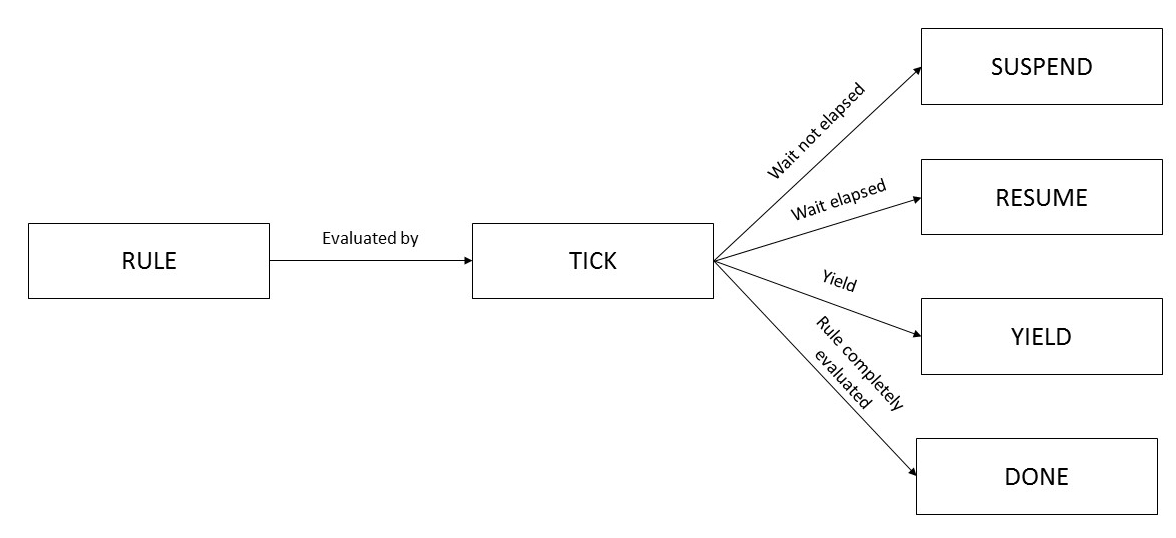
\includegraphics[width=\textwidth]{Figures/tick}
	\caption{Possible results of the \texttt{tick} function}
	\label{fig:ch_mcnv_languages_tick_result}
\end{figure}

\begin{lstlisting}
Data "rule" -> List[<<string>>] -> stmt -> stmt -> <<ImmutableDictionary<string, Value> >>  -> <<float>> : Rule
Data "Done" -> ctxt : ExecutionResult
Data "Suspend" -> stmt -> ctxt : ExecutionResult
Data "Yield" -> stmt -> List[Value] -> ctxt : ExecutionResult
Data "Resume" -> stmt -> ctxt : ExecutionResult
Data "Atomic" -> stmt -> ctxt : ExecutionResult
Func "tick" -> List[Rule] -> List[Rule] -> 
	<<ImmutableDictionary<string, Value> >> -> <<ImmutableDictionary<string, Value> >> -> <<float>> : GameState   
\end{lstlisting}

\noindent
Note that in the implementation we use a generic meta-data structure \texttt{List} instantiated with the meta-type \texttt{Rule}. A \texttt{rule} is a meta-data structure containing a list of strings representing the domain, a sequence of statements representing the rule body, a second sequence of statement representing the continuation (i.e. the statements to be evaluated in the next frame), a symbol table of local variables, and the frame time difference.

As stated above, the \texttt{tick} function stops when all the rules have been evaluated, thus when both lists of rules are empty. In this case we return the unchanged state of the program:

\begin{lstlisting}
--------------------------------------------
tick nil nil fields globals dt -> (State nil fields globals)
\end{lstlisting}

When the rule evaluation returns \texttt{Resume}, we build a rule containing the code to execute at the next frame, when the rule restarts, an empty continuation, because the current one has been moved into the body of the new rule, and the updated symbol table, since generally the rule evaluation might define some local variables. We then recursively update the remaining rules, and finally we build a new state with the rule that has to been resumed and all the other updated rules, that are stored in the state returned by the recursive call. Note that we will present the detail of \texttt{evalRule} further ahead.

\begin{lstlisting}
evalRule (rule dom body k locals delta) fields globals -> Resume cont (Context newLocals newFields newGlobals)
r := rule dom cont nop newLocals dt
tick originals rs newFields newGlobals dt -> (State updatedRules updatedFields updatedGlobals)
st := State (r::updatedRules) updatedFields updatedGlobals
------------------------------------------------------
tick (original::originals) ((rule dom body k locals delta)::rs) fields globals dt -> st
\end{lstlisting}

\noindent
For instance, consider the rule in Listing \ref{code:ch_mcnv_languages_rule_example} and assume that \texttt{dt = 1.0}.

\begin{lstlisting}[caption = Rule example with interruption, label = code:ch_mcnv_languages_rule_example]
rule X =
  wait 1.0f
  yield X + 1
\end{lstlisting}

\noindent
After evaluating the \texttt{wait} statement, the rule evaluation would return \texttt{Resume} containing the following continuation:

\begin{lstlisting}
cont = yield X + 1
\end{lstlisting}

\noindent
The new rule that will be generated is therefore

\begin{lstlisting}
rule X =
  yield X + 1
\end{lstlisting}

\noindent
In the case of \texttt{Yield} the procedure is analogous, since \texttt{yield} pauses the rule execution for one frame and thus the continuation must be used to rebuild a new rule with the continuation in its body.

\begin{lstlisting}
evalRule (rule dom body k locals delta) fields globals -> Yield cont values (Context newLocals newFields newGlobals)
r := rule dom cont nop newLocals dt
tick originals rs newFields newGlobals dt -> (State updatedRules updatedFields updatedGlobals)
st := State (r::updatedRules) updatedFields updatedGlobals
------------------------------------------------------
tick (original::originals) ((rule dom body k locals delta)::rs) fields globals dt -> st
\end{lstlisting}

For instance, let us consider again the rule

\begin{lstlisting}
rule X =
  yield X + 1
\end{lstlisting}

\noindent
Its evaluation will generate a rule with an empty body, such as

\begin{lstlisting}
rule X = nop
\end{lstlisting}

\noindent
When the rule evaluation returns \texttt{Done}, it means that the rule statements have been completely evaluated. In this case the rule must pause for one frame. It is also necessary to rebuild the body of the rule as it was before its execution started. Indeed, during the execution, the rule body is ``broken'' when evaluating the body because the executed statements are thrown away during the recursive calls. In the previous examples we have seen this process in action (see Listing \ref{code:ch_mcnv_languages_rule_example}). As we can see in the meta-language rule below, this time we build a new set of rules by placing the rule in its original state.

\begin{lstlisting}
evalRule r fields globals -> Done (Context newLocals newFields newGlobals)
tick originals rs newFields newGlobals dt -> (State updatedRules updatedFields updatedGlobals)
st := State (original::updatedRules) updatedFields updatedGlobals
--------------------------------------------------------------
tick (original::originals) (r::rs) fields globals dt -> st
\end{lstlisting}

\noindent
Finally, when the rule evaluation returns \texttt{Suspend}, we obtain the updated state of the \texttt{wait} statement (when the timer is updated) and a continuation. In this case we rebuild a rule whose body contains the updated \texttt{wait} statement and the continuation. 

\begin{lstlisting}
evalRule (rule dom body k locals delta) fields globals -> Suspend (s;cont) (Context newLocals newFields newGlobals)
r := rule dom s cont newLocals dt
tick originals rs newFields newGlobals dt -> (State updatedRules updatedFields updatedGlobals)
st := State (r::updatedRules) updatedFields updatedGlobals
------------------------------------------------------
tick (original::originals) ((rule dom body k locals delta)::rs) fields globals dt -> st
\end{lstlisting}

\noindent
For instance, consider again the rule in Snippet \ref{code:ch_mcnv_languages_rule_example} but this time with \texttt{dt = 0.5}. The rule update this time returns \texttt{Suspend} (because the timer has not elapsed yet) with:

\begin{lstlisting}
s = wait 0.5f
cont = yield X + 1
\end{lstlisting} 

\noindent
thus the new rule will look like:

\begin{lstlisting}
rule X =
  wait 0.5f
  yield X + 1
\end{lstlisting}

\noindent
A summary of this process can be seen in Figure \ref{fig:ch_mcnv_languages_tick}.

\begin{figure}
	\centering
	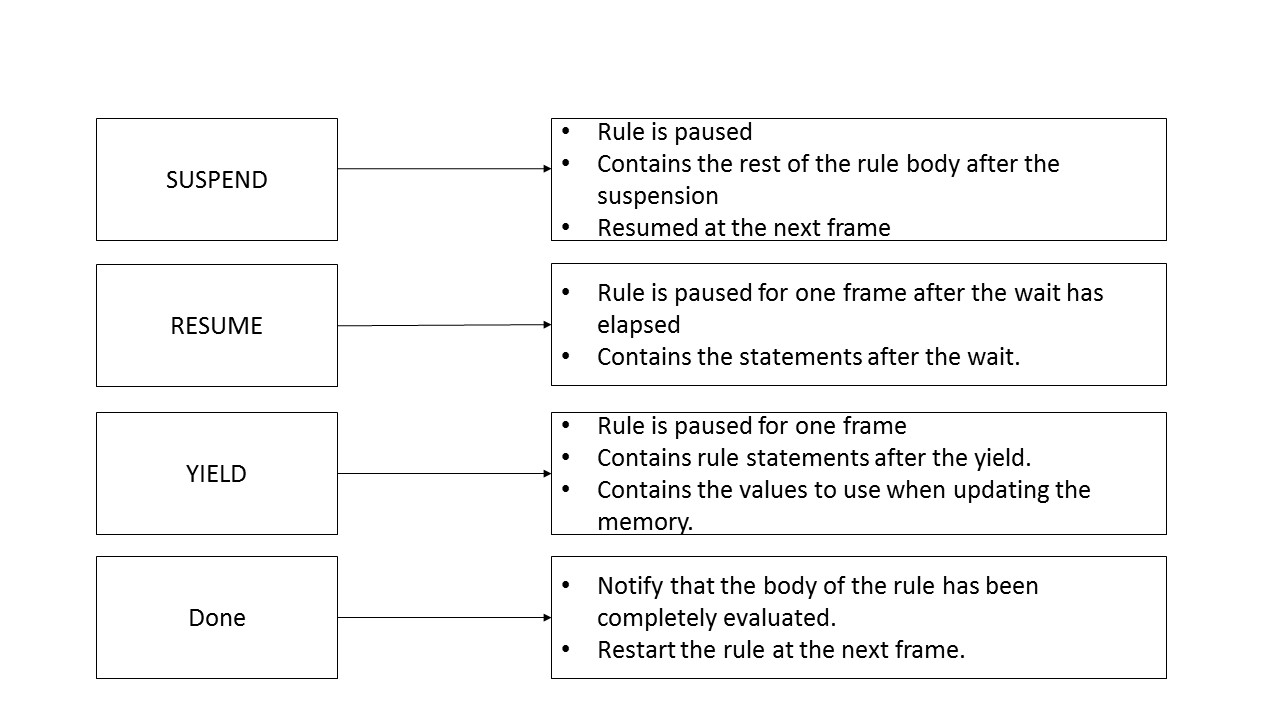
\includegraphics[width=\textwidth]{Figures/tick2}
	\caption{Cases of rule update}
	\label{fig:ch_mcnv_languages_tick}
\end{figure}

\subsection{Rule evaluation}
\label{subsec:ch_mcnv_languages_rule_evaluation}

The function \texttt{evalRule} takes as input a rule and the symbol tables for the current entity and the \texttt{world} and returns an execution result, as seen in Section \ref{subsec:ch_mcnv_languages_rule_update}.

\begin{lstlisting}
Func "evalRule" -> Rule -> <<ImmutableDictionary<string, Value> >> -> <<ImmutableDictionary<string, Value> >> : ExecutionResult
\end{lstlisting}

\noindent
Semantics rules having \texttt{evalRule} in their conclusion call in one of their premises the function \texttt{eval\tu s}. This function is able to process a sequence of statements and return a result depending on the current statement being executed. When \texttt{eval\tu s} returns \texttt{Done}, \texttt{Suspend}, or \texttt{Resume}, \texttt{evalRule} simply forwards the result to \texttt{tick} as it is. On the other hand, \texttt{eval\tu s} can also return \texttt{Yield} and an additional result called \texttt{Atomic}. This kind of result represents a statement that does not pause the rule execution. \texttt{Atomic} statements are evaluated within the current frame until an interruption statement or the end of the rule is reached.

In the case of \texttt{Yield}, the function must update the fields of the entity before returning the result to \texttt{tick}, as shown below:

\begin{lstlisting}
eval_s b k (Context locals fields globals) dt -> Yield ks values context
updateFields dom values context  -> updatedContext
-----------------------------------------
evalRule (rule dom b k locals dt) fields globals -> Yield ks values updatedContext
\end{lstlisting}

\noindent
We omit the implementation details of \texttt{updateFields} for brevity; suffice to say that this function evaluates the expressions contained in \texttt{yield} and writes their values in the symbol table.

In the case of \texttt{Atomic}, the rule must immediately be re-evaluated in the current frame. This is obtained by recursively calling \texttt{evalRule} again with the current rule whose body has been replaced by the continuation returned by \texttt{Atomic} (which is simply the remaining code in the rule body).

\begin{lstlisting}
eval_s b k (Context locals fields globals) dt -> Atomic z (Context newLocals newFields newGlobals)
evalRule (rule dom z nop newLocals dt) newFields newGlobals -> res
-----------------------------------------
evalRule (rule dom b k locals dt) fields globals  -> res
\end{lstlisting}

A schematic representation of the interaction between \texttt{tick} and \texttt{evalStatement} can be seen in Figure \ref{fig:ch_mcnv_languages_rule_update}.

\begin{figure}
	\centering
	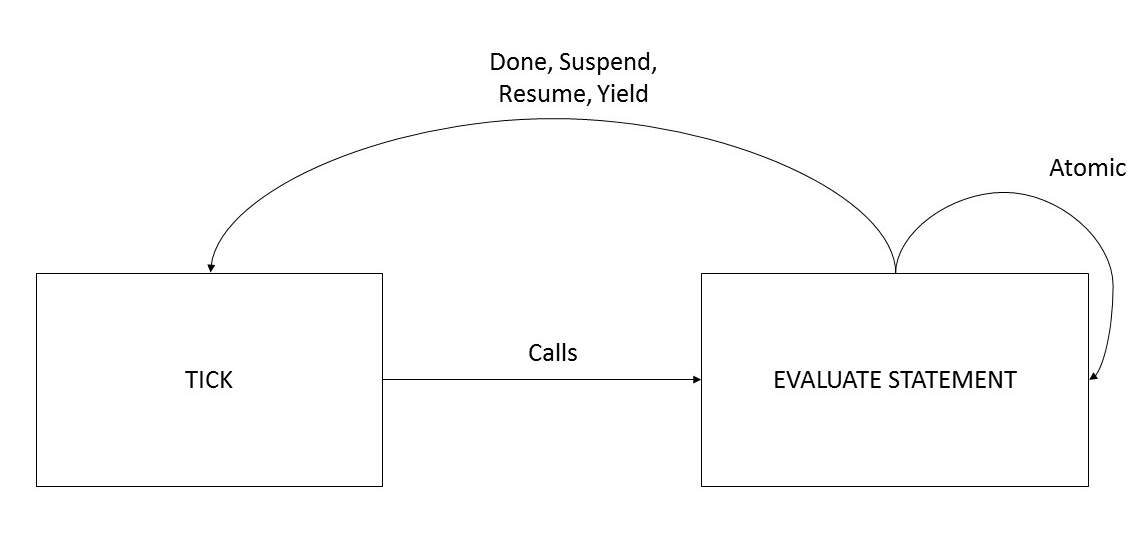
\includegraphics[width=\textwidth]{Figures/statement_evaluation}
	\caption{Rule update in Metacasanova}
	\label{fig:ch_mcnv_languages_rule_update}
\end{figure}

\subsection{Statement evaluation}
Statement evaluation is implemented through the function \texttt{eval\tu s}. This function takes as input a sequence of statements or a single statement and returns a different result depending on the statement semantics. This function takes as input the current body of the rule, its continuation and the context of the program made by the symbol tables of \texttt{world}, the current entity, and the local variables of the rule.

\begin{lstlisting}
Func "eval_s" -> stmt -> stmt -> ctxt -> <<float>> : ExecutionResult
\end{lstlisting}

\noindent
The base case of \texttt{eval\tu s} is when the body of the rule is empty and there is no continuation. This is the case when the whole rule body has been executed and thus we have to return \texttt{Done}.

\begin{lstlisting}
-------------------------------
eval_s nop nop ctxt dt -> Done ctxt
\end{lstlisting}

\noindent
When the rule body is non-empty, then we must extract the first statement in the statement sequence. We then combine the remaining body of the rule with the current continuation into a single statement sequence by using the function \texttt{addStmt}. This function has two cases: (\textit{i}) both the remaining body of the rule and the continuation are empty, or (\textit{ii}) the body of the rule is non-empty. The first case happens when we are executing the last statement in the rule body. In this case we generate an empty continuation containing \texttt{nop}. In the second case we simply combine the remaining body of the rule and the continuation into a single statement sequence.

\begin{lstlisting}
a != nop
---------------------
addStmt a b -> a;b

-------------------
addStmt nop nop -> nop
\end{lstlisting}

\noindent
Note that the case where only \texttt{b} is \texttt{nop} cannot be generated, because executing a statement will always generate a non-empty continuation, unless it is the last statement of the rule to be executed. This case is captured by \texttt{eval\tu s} (as shown above), which will return \texttt{Done}. When \texttt{Done} is forwarded as result to \texttt{tick}, the body of the rule will be regenerated by replacing it with the initial code of the rule (we reset the rule) as shown in Section \ref{subsec:ch_mcnv_languages_rule_update}.

After the new continuation has been generated, we recursively call \texttt{eval\tu s} by giving it as input the first statement in the rule body.

\begin{lstlisting}
addStmt b k -> cont
eval_s a cont ctxt dt -> res
-------------------------------
eval_s (a;b) k ctxt dt -> res
\end{lstlisting}

We now proceed to show how the semantics of the statements is implemented

\subsubsection{Interruptible statements}
Interruptible statements are statements that can pause the execution of a rule: \texttt{wait} and \texttt{yield}. As briefly pointed out before, \texttt{yield} returns as result a meta-data structure \texttt{Yield} containing the continuation of the rule to resume at the next frame, the values to write in the domain fields, and the current program context (the symbol tables). Since the arguments of \texttt{yield} can be expressions, its semantics must evaluate them one by one and return their values.

\begin{lstlisting}
-------------------------
evalYield nil ctxt -> nil

eval expr ctxt -> v
evalYield exprs ctxt -> vs
-------------------------------------------
evalYield (expr :: exprs) ctxt -> v :: vs


evalYield exprs ctxt -> values
------------------------------------------------------
eval_s (yield exprs) k ctxt dt -> Yield k values ctxt
\end{lstlisting}

\noindent
The statement \texttt{wait} in Casanova has double semantics: one waits for a timer to elapse and the other until a certain condition is met. In Metacasanova we do not have overloading, thus we are forced to use a different name to model both cases of its semantics. We use \texttt{wait} for the timed and \texttt{when} for the conditional version of the statement.

For the timed version we have two cases: (\textit{i}) the timer has elapsed and we can resume the execution of the rule at the next frame, or (\textit{ii}) the timer is still running, thus we have to suspend the rule. In the first case we return \texttt{Resume} containing the current continuation of the rule body. In the other case we have to suspend the rule, thus we return \texttt{Suspend} where the continuation contains \texttt{wait}, whose timer has been updated by removing \texttt{dt}, concatenated to the current continuation of the rule.

\begin{lstlisting}
eval expr ctxt -> ($f t)
t > dt
<<t - dt>> -> t'
----------------------------------
eval_s (wait expr) k ctxt dt -> Suspend (wait $f t');k ctxt

eval expr ctxt -> ($f t)
t <= dt
----------------------------------
eval_s (wait expr) k ctxt dt -> Resume k ctxt
\end{lstlisting}

\noindent
The implementation of \texttt{when} is analogous: if the condition is not met then we simply return \texttt{Suspend} where the continuation contains \texttt{when} concatenated with the previous continuation. Otherwise we return \texttt{Resume} containing the current continuation.

\begin{lstlisting}
eval expr ctxt -> ($b true)
---------------------------------------------
eval_s (when expr) k ctxt dt -> Atomic k ctxt

eval expr ctxt -> ($b false)
------------------------------------------
eval_s (when expr) k ctxt dt -> Suspend (when expr);k ctxt
\end{lstlisting}

\subsubsection{Control strucutres}
Casanova supports a conditional control structure (\texttt{if-then-else}), and two iterative control structures (\texttt{while-do} and \texttt{for-do}). The only difference with the usual semantics of control structures lies in \texttt{for-do}, which is like that of Python and F\# as it takes as input a variable that is used to iterate through the elements of a list.

The implementation of the control structures is similar to that of C-{}- with the difference that their body can be interrupted as well. At this purpose, the semantics rules must generate an appropriate continuation that will be handled by \texttt{tick}. The conditional control structure checks if the condition is true or false to select the appropriate code block to execute. After that it returns an \texttt{Atomic} result containing the concatenation of the selected code block with the current continuation of the rule. This is because the evaluation of the condition is an atomic process, i.e. must not pause the execution of the rule. The first statement of the selected code block will be executed immediately after.

\begin{lstlisting}
eval cond ctxt -> $b true
-----------------------------------------------------------
eval_s (if cond then b else c) k ctxt dt -> Atomic b;k ctxt

eval cond ctxt -> $b false
-----------------------------------------------------------
eval_s (if cond then b else c) k ctxt dt -> Atomic c;k ctxt
\end{lstlisting}

\noindent
\texttt{while-do} follows the same behaviour described in C-{}-, thus if the condition is false we simply skip the loop, otherwise we execute the body followed by the same loop. This time we must encapsulate the code built after the evaluation of the condition in an \texttt{Atomic} result, because the body must be immediately evaluated after checking the condition, as for conditionals.

\begin{lstlisting}
eval cond ctxt -> $b true
----------------------------------------------
eval_s (while cond b) k ctxt dt -> Atomic b;((while cond b);k) ctxt

eval cond ctxt -> $b false
----------------------------------------------
eval_s (while cond b) k ctxt dt -> Atomic k ctxt
\end{lstlisting}

\noindent
The semantics of \texttt{for-do} loop are quite different than what we had defined for C-{}-. The loop defines a variable that is used to iterate each element of a list. The list can be given directly or be an expression that returns a list. Thus, we have to first add to the local variables the one defined in the loop, then evaluate the expression for the list, and finally evaluate the body of the loop itself. Note that lists here are considered lists in the Casanova language and not lists of Metacasanova (thus they are values in Casanova and not meta-data structures).

\begin{lstlisting}
eval expr ctxt -> ($l nil)
------------------------------------------
eval_s (for v in expr b) k ctxt dt -> Atomic k ctxt

eval expr (Context locals e w) -> ($l (x :: xs))
locals add var x -> updatedLocals
-------------------------------------
eval_s (for ($ var) in expr b) k (Context locals e w) dt -> Atomic b;((for ($ var) in ($l xs) b);k) (Context updatedLocals e w)
\end{lstlisting}

\noindent
The base case of the evaluation is when the list is empty. In this case we simply return \texttt{Atomic} containing the current continuation because the loop can be skipped. The recursive case is when the list is non-empty: in this case we first evaluate the expression of the list, then we add the variable defined in the loop to the local variables, assigning it the value of the head of the list. We finally return an \texttt{Atomic} that contains a continuation where the body of the loop is concatenated to the loop itself and the current continuation. \texttt{Atomic} will also contain a program context where the locals now contain the new variable defined in the loop.

Note that, for simplicity, we do not have code block scoping like in C-{}-. This feature can be implemented by replacing the local symbol table with a list of tables as previously shown in Section \ref{subsec:ch_mcnv_languages_expression_semantics}.

\section{Evaluation}
\label{sec:ch_mcnv_languages_evaluation}
In this section we compare the runtime performance of a program written for C-{}- and Casanova implemented in Metacasanova with their equivalent implementation in Python. Moreover, we evaluate the length of the language definition in Metacasanova with respect to their hard-coded implementation. We begin by describing the experimental set-up, we proceed by explaining how we analyse the results, and then we discuss them

\subsection{Experimental Set-up}
We evaluated C-{}- and the meta-compiled Casanova runtime performance against an equivalent implementation of equivalent programs in Python. C-{}- was tested running a program to compute the factorial, while we implemented a program in Metacasanova where some entities patrol an area according to pre-defined checkpoints. In the case of Casanova, this language was chosen based on its use in game development: Python has been used extensively in several games such as Civlization IV \cite{CIV4} or World in Conflict \cite{WIC} because of the native support for coroutines that allow to implement a behaviour similar to that of Casanova rules. In the case of C-{}-, we still use Python because, as we discuss further ahead, the behaviour of this language is much more similar to that of a dynamic language (the name was chosen mainly because of a lack of creativity from the author than because of its similarity with C). As for the code length, we compare the length of the semantics definition of C-{}- with a hard-coded implementation, while we compare the definition of Casanova in Metacasanova with respect to its hard-coded compiler written in F\#.

For Casanova we use a program where a Casanova entity patrols a set of checkpoints. When the entity reaches the position of a checkpoint it will move to the next one. The same code has been re-implemented in Python using coroutines to simulate the interruption mechanism of rule statements that is built-in in Casanova. The code generated by the version of Casanova implemented in Metacasanova was imported in a C\# program for Monogame but tested in isolation to actually measure only the running time of the logic, which would otherwise be influenced by the rendering time and the overhead of Monogame itself. We run the Casanova program and the Python version with a variable number of entities (that will be updated) ranging from 100 to 250. For each execution we measure the time taken to update them all for each frame, and we average this time on the number of total frames. As for the code length of the language definition, we measure the length of the language specification in Metacasanova and we compare it with the relative parts of code in the hard-coded version of the compiler.

This code has also been tested by including it in a Monogame project. The program code generated with the Metacompiler updates the logic of the entities that are drawn using the Monogame framework. In this way the logic of the game is written in the meta-compiled version of Casanova and the external framework is used only for the graphical part. This has the advantage that the same code can be re-used in another game engine that is able to run .NET code (for instance Unity). A schematic representation of the integration with Monogame is shown in Figure \ref{fig:ch_mcnv_languages_monogame_integration}

\begin{figure}
	\centering
	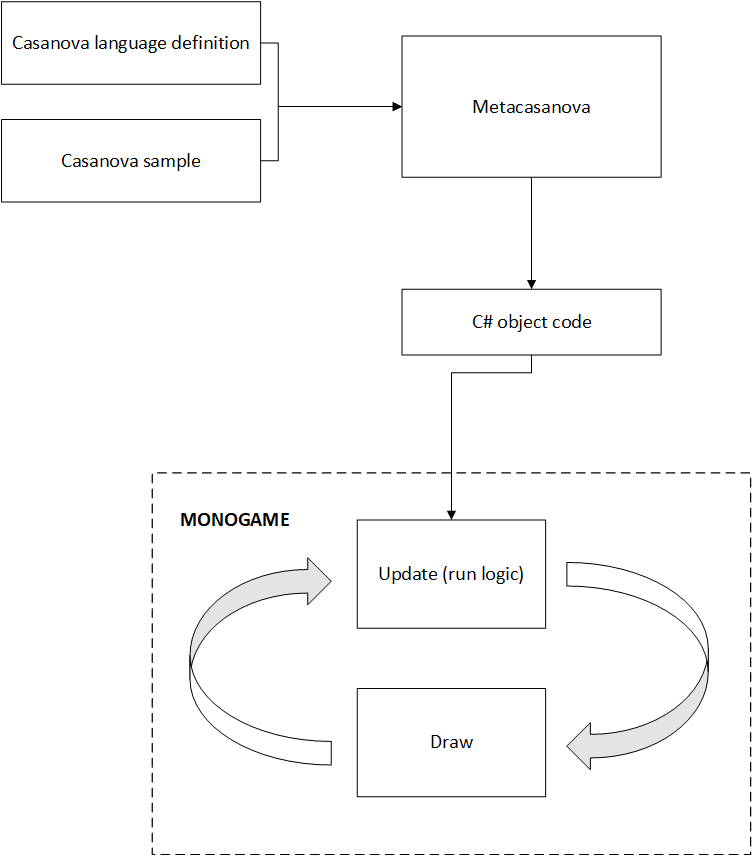
\includegraphics[width = \textwidth]{Figures/chapter_languages/monogame_integration}
	\caption{Integration of meta-compiled Casanova in Monogame}
	\label{fig:ch_mcnv_languages_monogame_integration}
\end{figure}

\subsection{Performance}
From Table \ref{tab:ch_mcnv_languages_casanova_compiler_comparison} we see that the implementation of Casanova 2.0 language in Metacasanova is almost 5 times shorter in terms of lines of code than the hard-coded implementation of the Casanova compiler written in F\#, while the C-{}- implementation is 11 times shorter (Table \ref{tab:mcnv_languages_cmm}). We believe it is worthy noticing that structures with complex behaviours, such as \textit{wait} or \textit{when}, require hundreds of lines of codes with a standard approach (the code lines to define the behaviour of the structure plus the support code to correctly generate the state machine), while in the meta-compiler we just need tens of lines of codes to implement the same behaviour. Moreover we want to point out that the previous Casanova compiler was written in a functional programming language: these languages tend to be more synthetic than imperative languages, so the difference with the same compiler implemented in languages such as C/C++ might be even greater.

The readability with respect to the hard-coded compiler code is also improved: we managed to implement the behaviour of synchronization and timing primitives almost imitating one to one the formal semantics of the language definition. In the hard-coded compiler implementation for Casanova 2.0 the semantics are lost in the code for generating finite state machines. Just for comparison, Figure \ref{fig:ch_mcnv_languages_wait_code_generation} shows the code from the Casanova hard-coded compiler to generate part of the state machine necessary to simulate the behaviour of the timed version of \texttt{wait} (the code generation of \texttt{when} has about the same size).

\begin{figure}
	\centering
	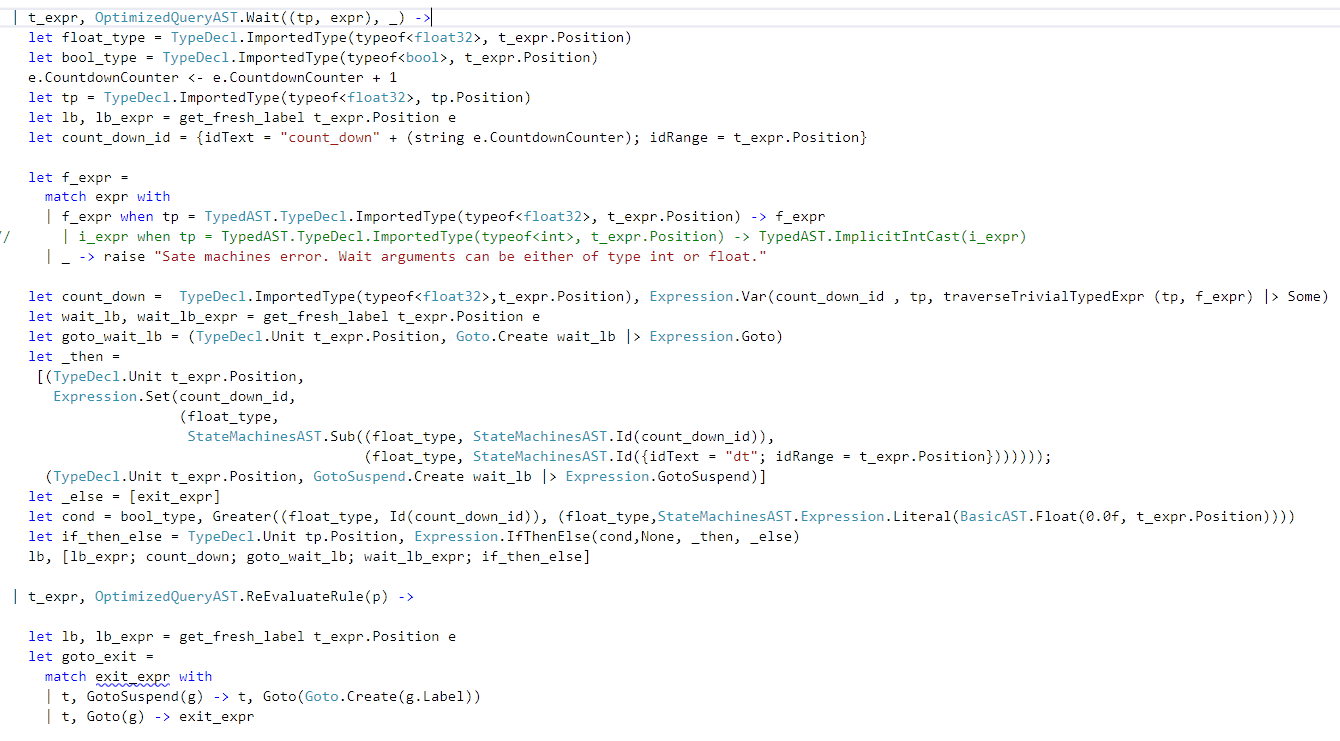
\includegraphics[angle = 90,scale= 0.6]{Figures/wait_code_casanova_compiler}
	\caption{Code generation of \texttt{wait} in the Casanova compiler}
	\label{fig:ch_mcnv_languages_wait_code_generation}
\end{figure}

The performance results are shown in Table \ref{tab:ch_mcnv_casanova_evaluation}. We see that the generated code has performance on the same order of Python, although 3 times slower. This gap is accentuated in the case of C-{}-, which is 50 times slower than Python, because in the case of a simple imperative program, where the use of virtual tables for polymorphic types (as coroutines) is limited, the speed of Python greatly increases.

\begin{table}
	\centering
	\begin{tabular}{|c|c|c|}
		\hline
		\multicolumn{3}{|c|}{\textbf{Casanova 2.5}} \\
		\hline
		Entity \# & Average update time (s) & Frame rate \\
		\hline
		100 & 0.00349 & 286.53 \\
		\hline
		250 & 0.00911 & 109.77 \\
		\hline
		500 & 0.01716 & 58.275 \\
		\hline
		750 & 0.02597 & 38.506 \\
		\hline
		1000 & 0.03527 & 28.353 \\
		\hline
		\multicolumn{3}{|c|}{\textbf{Python}} \\
		\hline
		Entity \# & Average update time (s) & Frame rate \\
		\hline
		100 & 0.00132 & 756.37 \\
		\hline
		250 & 0.00342 & 292.05 \\
		\hline
		500 & 0.00678 & 147.54 \\
		\hline
		750 & 0.01087 & 91.988 \\
		\hline
		1000 & 0.01408 & 71.002 \\
		\hline
	\end{tabular}
	\caption{Patrol sample evaluation}
	\label{tab:ch_mcnv_casanova_evaluation}
\end{table}

\begin{table}
	\centering
	\begin{tabular}{|c|c|}
		\hline
		\multicolumn{2}{|c|}{\textbf{Casanova 2.5 with Metacasanova}} \\
		\hline
		Module & Code lines \\
		\hline
		Data structures and function definitions & 40 \\
		\hline
		Query Evaluation & 16 \\
		\hline
		While loop & 4 \\
		\hline
		For loop & 5 \\
		\hline
		If-then-else & 4 \\
		\hline
		When & 4 \\
		\hline
		Wait & 6 \\
		\hline
		Yield & 10 \\
		\hline
		Additional rules for Casanova program evaluation & 40 \\
		\hline
		Additional rules for basic expression evaluation & 201 \\
		\hline
		\multicolumn{2}{|l|}{\textbf{Total: } 300} \\
		\hline
		\multicolumn{2}{|c|}{\textbf{Casanova 2.0 compiler}} \\
		\hline
		Module & Code lines \\
		\hline
		While loop & 10 \\
		\hline
		For-loop and query evaluation & 44 \\
		\hline
		If-Then-Else & 15 \\
		\hline
		When & 11 \\
		\hline
		Wait & 24 \\
		\hline
		Yield & 29 \\
		\hline
		Additional structures for rule evaluation & 63 \\
		\hline
		Structures for state machine generations & 754 \\
		\hline
		Code generation & 530 \\
		\hline
		\multicolumn{2}{|l|}{\textbf{Total: } 1480} \\
		\hline			
	\end{tabular}	
	\caption{meta-compiler vs standard compiler}
	\label{tab:ch_mcnv_languages_casanova_compiler_comparison}
\end{table}

\begin{table}
	\centering
	\begin{tabular}{|c|c|c|}
		\hline
		\textbf{Statement} & \textbf{Metacasanova} & \textbf{C\#}\\
		\hline
		\texttt{if-then-else} & 4 & 103 \\
		\hline
		\texttt{while} & 7 & 73 \\
		\hline
		\texttt{For} & 11 & 81\\
		\hline
	\end{tabular}
	
	\vspace{0.15cm}
	\begin{tabular}{|c|c|}
		\hline
		\textbf{C-{}-} & \textbf{Python} \\
		\hline
		1.26ms & $2.36 \cdot 10^{-2}$ms \\
		\hline
	\end{tabular}
	\caption{Code length implementation of C-{}- and run-time performance}
	\label{tab:mcnv_languages_cmm}
\end{table}

\subsection{Discussion}
\label{subsec:code_generation_discussion}
Even though the size of the code required to implement the language has been drastically reduced (almost 1/5 shorter), performance dropped dramatically. The problem lies in the fact that, in order to implement a memory model, in the current version of Casanova we must rely on dynamic access to a symbol table at runtime. Indeed, when we define a new variable or read its value, the semantics contain a rule defining the insertion or the lookup of the variable. Metacasanova generates the code able to run those rules, but the memory operations are thus executed at runtime as dictionary operations.

In order to encode a symbol table in the meta-compiler in the current implementation (used for example to store the variables defined in the local scope of a control structure or to model a class/record data structure), we are left with two options: (\textit{i}) define a custom data structure made of a list of pairs, containing the field/variable name as a string and its value, in the following way

\begin{lstlisting}
Data "table" -> List[Tuple[string, Value]] : SymbolTable
\end{lstlisting}

\noindent
or (\textit{ii}) use a dictionary data structure coming from .NET, such as\\ \texttt{ImmutableDictionary}, which was the implementation choice for Casanova. In both cases, the behaviour of the language implemented in Metacasanova will be that of a dynamic language, because whenever the value of a variable or class field must be read, the evaluation rule must look up the symbol table at run time to retrieve the value, whose complexity will be $O(n)$ with the list implementation and $O(\log n)$ with the dictionary implementation.

The same applies to type checking: in Section \ref{subsec:ch_mcnv_languages_type_checking} we showed the type rules that check the types of a C-{}- program. In statically-typed languages, type checking is usually performed at compile time and not at runtime. However, in this case Metacasanova will again generate the code to run the type rules, but the actual execution is performed when the program is run, thus the behaviour of C-{}- is more similar to that of a dynamic language rather than a static language (and its performance as well).

This issue is caused by the fact that, in the current state of Metacasanova, the meta-type system is unaware of the type system of the language that is being implemented in the meta-compiler. This means that, as it is, the meta-language is unable to define a statically-typed language. This is not a problem limited to Metacasanova but to all meta-compilers having a meta-type system that does not allow embedding of the host language type system. 

The same applies for the lookup: the access to symbol tables needs not to be dynamic because the symbol table does not grow when the program runs, thus the access to a specific variable could be directly inlined in the code. For example, if we want to access variable \texttt{x}, which is the third entry of the symbol table, we will always perform the same lookup. Thus, this lookup could be simply inlined as an access to the third element of the symbol table. An analogous situation happens for Casanova entities: their structure does not change at runtime, so if we access, for instance, a field \texttt{Velocity} of an entity and that is the third one, then we always perform a lookup on the third element of the symbol table, and this can be inlined directly as well.

\section{Summary}
In this chapter we showed two examples of how to use Metacasanova to implement programming languages. We started by showing how to implement a small imperative language called C-{}-. We showed an implementation of its semantics and then of its type system. Later we re-implemented the Casanova language, a DSL for game development. We showed how to implement the semantics of interruptible code, which in Casanova had been implemented with state machines, by using continuation-passing style. Metacasanova implementation of Casanova results to be 5 times shorter than that of the hard-coded compiler for Casanova written in F\#. In the case of C-{}- the gap in terms of lines of code is even larger, being the code for its semantics 11 times shorter than a hard-coded implementation. However, the code performance drops dramatically: testing the meta-compiled version of Casanova against Python results in its code being 3 times slower (although on the same order of magnitude), while the C-{}- code is even 50 times slower. The cause of this is that, even thought these languages could be statically-typed, the rule evaluation performs the lookup of variables and types at runtime. This cannot be changed with the Metacasanova language abstractions presented so far because the meta-type system of Metacasanova is unaware of the types of the embedded language (i.e. the language that is being implemented in Metacasanova). In the next chapter we will show a language extension for Metacasanova that relies on \textit{Functors} to embed the type system of languages implemented in Metacasanova in its type system, and to inline the access to variables at compile time.

\chapter{Metacasanova Optimization}
\label{ch:functors}
\epigraph{First you learn the value of abstraction, then you learn the cost of abstraction, then you're ready to engineer.}{Kent Beck}
In Chapter \ref{ch:metacasanova} and \ref{ch:languages} we have presented the Metacasanova metacompiler and its meta-language and shown how to implement with it a small imperative language, C-{}-, and a DSL for game development, Casanova. The performance analysis showed that, although the development effort for the language compilers was greatly reduced by using Metacasanova, this has come at the cost of performance. The performance decay is due to the fact that the meta-type system of Metacasanova is unaware of the type system of C-{}- or Casanova. This requires all the type checking and access to data structures to be performed at runtime, thus making a statically-typed language exhibit the behaviour and performance of dynamically typed languages. In this chapter we propose a language extension \cite{DiGiacomo2017SLE} for Metacasanova that is designed to overcome the problem of performance decay and dynamic checks. In this context we use the term \textit{embedded language} to refer to a language that is being implemented in Metacasanova and \textit{embedded program} for a program implemented in an embedded language.

\section{Language extension idea}
\label{sec:ch_functors_idea}
The experimental results from Chapter \ref{ch:languages} showed that the performance of Metacasanova is strongly affected by the dynamic type checks and symbol table access at runtime. This is necessary because Metacasanova generates the code necessary to evaluate the semantics of accessing the value of a variable in the symbol table that mimics the behaviour of rules in natural semantics, but such evaluation is performed at runtime. However the runtime evaluation is necessary only because of the limitations of the language presented so far, as Metacasanova is not able to build a symbol table while compiling the meta-program. This should not be the case since

\begin{enumerate}
	\item The symbol table of a statically-typed language does not grow at runtime because it is built during the compilation.
	\item The position of an entry for a variable in the symbol table does not change during the program execution, thus every time we perform an access to the same variable, we access the very same element in the symbol table.
\end{enumerate}

\noindent
Analogously, type checking in a statically-typed language is performed at compilation time rather than at runtime, which happens in dynamic languages such as Python. Metacasanova is forced to do runtime type checking because, at compilation time, the metacompiler only checks for the meta-types, i.e. the types of the language abstractions defined in the meta-language, but not for the program structures of the embedded program itself. This would require to be able to embed the type system of the embedded language into the meta-type system of Metacasanova. In this way the type checker of Metacasanova would be able to check at the same time the types of both the meta-program and of the embedded program. 

To better clarify what stated so far we show in the following section an example of what happens when accessing the field of a Casanova entity with the implementation given in Chapter \ref{ch:languages}. We then proceed to show the idea of a possible solution to overcome the performance decay.

\subsection{Field access in Casanova}
\label{subsec:ch_functors_casanova_example}
As we showed in Section \ref{subsec:ch_mcnv_languages_casanova_semantics}, an entity in Casanova embedded in Metacasanova is represented via a map where the key is the field name and the value is the value currently stored in the field. This representation is very similar to that of records or classes. Let us consider the following entity representing a physical body consisting of a \texttt{Position} and a \texttt{Velocity} in a 2D space:

\begin{lstlisting}
type PhysicalBody = {
  Position        : Vector2
  Velocity        : Vector2
}
\end{lstlisting}

\noindent
and the following rules for \texttt{PhysicalBody}

\begin{lstlisting}
rule Position = Position + Velocity * dt

rule Position =
  if Position.X > 500f then
    yield new Vector2(500f,Position.Y)
  elif Position.X < 0f then
    yield new Vector2(0f,Position.Y)
  elif Position.Y < 0f then
    yield new Vector2(Position.X,0f)
  elif Position.Y > 500f then
    yield new Vector2(Position.X,500f)
\end{lstlisting}

The first rule simply updates the position using the Euler approximation of the differential equation for the velocity

\begin{equation*}
v(t) = \dfrac{ds(t)}{dt}
\end{equation*}

\noindent
while the second rule ensures that the physical body does not exit a specific area, which could represent the playable area in a 2D game.

Assuming that the physical body is in position $(10,10)$, it is represented in Metacasanova via a map as shown in Table \ref{tab:ch_functors_physical_body}.

\begin{table}
	\centering
	\begin{tabular}{|c|c|}
		\hline
		\textbf{Field} & \textbf{Value} \\
		\hline
		Position	& 10 \\
		\hline
		Velocity & 10 \\
		\hline
	\end{tabular}
	\caption{Meta-representation of the physical body}
	\label{tab:ch_functors_physical_body}
\end{table}

\noindent
The Metacasanova semantics rule that evaluates the first Casanova rule will evaluate the expression in its body by accessing respectively the field \texttt{Position} and \texttt{Velocity} to compute the expression value. It then stores the expression value in \texttt{Position} as shown in Table \ref{tab:ch_functors_physical_body_access1_1}.

\begin{table}
	\centering
	\begin{tabular}{c|c|c|}
		\cline{2-3}
		& \textbf{Field} & \textbf{Value} \\
		\cline{2-3}
		$\Rightarrow$ & \cellcolor{green}{Position}	& \cellcolor{green}{10,10} \\ 
		\cline{2-3}
	  & Velocity & 10,0 \\
		\cline{2-3}
	\end{tabular}
	
	\vspace{0.15cm}
	\begin{tabular}{c|c|c|}
		\cline{2-3}
		& \textbf{Field} & \textbf{Value} \\
		\cline{2-3}
	  & Position	& 10,10 \\ 
		\cline{2-3}
		$\Rightarrow$ & \cellcolor{green}{Velocity} & \cellcolor{green}{10,0} \\
		\cline{2-3}
	\end{tabular}
	
	\vspace{0.15cm}
	\begin{tabular}{c|c|c|}
		\cline{2-3}
		& \textbf{Field} & \textbf{Value} \\
		\cline{2-3}
		$\Rightarrow$ & \cellcolor{green}{Position}	& \cellcolor{green}{11,10} \\ 
		\cline{2-3}
		& Velocity & 10,0 \\
		\cline{2-3}
	\end{tabular}

	\caption{Memory access in the first rule of the Physical Body. We assume \texttt{dt = 0.1} and \texttt{Velocity = (10,0)}}
	\label{tab:ch_functors_physical_body_access1_1}
\end{table}

\begin{table}
	\centering
	\begin{tabular}{c|c|c|}
		\cline{2-3}
		& \textbf{Field} & \textbf{Value} \\
		\cline{2-3}
		$\Rightarrow$ & \cellcolor{green}{Position}	& \cellcolor{green}{\fbox{501},10} \\ 
		\cline{2-3}
		& Velocity & 10,10 \\
		\cline{2-3}
	\end{tabular}
	
	\vspace{0.15cm}
	\begin{tabular}{c|c|c|}
		\cline{2-3}
		& \textbf{Field} & \textbf{Value} \\
		\cline{2-3}
		$\Rightarrow$ & \cellcolor{green}{Position}	& \cellcolor{green}{501,\fbox{10}} \\ 
		\cline{2-3}
		& Velocity & 10,10 \\
		\cline{2-3}
	\end{tabular}
	
	\vspace{0.15cm}
	\begin{tabular}{c|c|c|}
		\cline{2-3}
		& \textbf{Field} & \textbf{Value} \\
		\cline{2-3}
		$\Rightarrow$ & \cellcolor{green}{Position}	& \cellcolor{green}{500,10} \\ 
		\cline{2-3}
		& Velocity & 10,10 \\
		\cline{2-3}
	\end{tabular}
	\caption{Memory access in the second rule of the Physical Body. We assume \texttt{Position.X = 501}}
\end{table}

As for the second rule, assuming that \texttt{Position.Y > 500f}, the rule will access \texttt{Position} three times: (\textit{i}) to evaluate the expression in the conditional, (\textit{ii}) to read \texttt{Position.Y} when instantiating a new vector, and (\textit{iii}) to write the new vector in \texttt{Position}. This situation is shown in Table

It should now appear clear that every time we need to read or write \texttt{Position} we access the first element of the table, while for \texttt{Velocity} we always access the second. In the following snippet we provide an alternative version of the code for the Casanova rules above that shows what really happens in Casanova embedded in Metacasanova :

\begin{lstlisting}
rule Position = PhysicalBodyTable[0] + PhysicalBodyTable[1] * dt
  
rule Position =
	if PhysicalBodyTable[0].X > 500f then
		yield new Vector2(500f,PhysicalBodyTable[0].Y)
	elif PhysicalBodyTable[0].X < 0f then
		yield new Vector2(0f,PhysicalBodyTable[0].Y)
	elif PhysicalBodyTable[0].Y < 0f then
		yield new Vector2(PhysicalBodyTable[0].X,0f)
	elif PhysicalBodyTable[0].Y > 500f then
		yield new Vector2(PhysicalBodyTable[0].X,500f)
\end{lstlisting}

Let us now assume that the program provides an invalid value for the update of \texttt{Position}:

\begin{lstlisting}
rule Position = "(10,10)"
\end{lstlisting}

\noindent
What would happen in embedded Casanova is that the type checker evaluates the type of the expression in the rule body, obtaining \texttt{string}. This type is then compared with that of \texttt{Position}, which is \texttt{Vector2}, and at this point an error would be reported. Again, this would require at runtime to access the first element of a symbol table containing type information about the entity fields. Note that all these lookups are not array accesses but rather dictionary accesses.

\subsection{Inlining the entity fields}
\label{subsec:ch_functors_inlining}
From the example above we can notice that, when the program runs, the symbol table used to represent a Casanova entity does not change, nor its entries change position. This means that every time we read or write the same field we perform the same access in the table. In the implementation provided in Section \ref{subsec:ch_mcnv_languages_casanova_semantics} this access requires the execution of a Metacasanova rule that is able to traverse the dictionary used for the entity symbol table and return the stored value. The traverse is performed every time, regardless of the fact that the field we are trying to access is indeed the same. Moreover, as it was also stated in Section \ref{sec:ch_mcnv_languages_evaluation}, we are looking at the very optimistic scenario where we make use of external .NET dictionaries to actually model the entity. If one had to rely solely on language abstractions defined in Metacasanova the symbol table should be modelled as a list of pairs containing field names, represented as strings, and meta-data structures representing values in the embedded language, introducing even a greater overhead. The physical body modelled in such way would then look like

\begin{lstlisting}
[("Position",(10,10)),("Velocity",(10,0)]
\end{lstlisting}

Accessing \texttt{Position} would then be performed by a Metacasanova rule that looks for the correct field name and stops when the field in this tuple has been reached:

\begin{lstlisting}
name = fieldName
----------------------------------
getField name ((fieldName,value) :: t) -> value

name <> fieldName
getField name t -> v
----------------------------------
getField name ((fieldName,value) :: t) -> v
\end{lstlisting}

\noindent
However the traversal of the tuple would always be the same when looking for a specific field, namely for \texttt{Position} the first Metacasanova rule will always be executed, while for \texttt{Velocity} the first time the second rule will be executed, which in turn recursively evaluates the remaining part of the list. The recursive call will then trigger the first rule at the second step. That being said, since the table does not grow and the access patterns are always the same, we could represent an entity as a nested tuple of pairs, in the fashion of Church encoding \cite{kleene1935theory, pierce2002types}, and inline in the code \texttt{fst PhysicalBodyTable} for \texttt{Position} and \texttt{fst(snd PhysicalBodyTable)} for \texttt{Velocity} whenever we require to access the respective fields, without repeating the same traversal every time. In this way the entity would look like:

\begin{lstlisting}
PhysicalBodyTable = ("Position",(10,10)),(("Velocity",(10,0)),())
\end{lstlisting}

\noindent
and thus \texttt{fst PhysicalBodyTable} (access to \texttt{Position}) would return\\ \texttt{("Position",(10,10))} and \texttt{fst(snd PhysicalBodyTable)} (access to\\ \texttt{Velocity}) would return \texttt{("Velocity",(10,0))}.

In the following sections we present the language extension required to allow this form of inlining and we show their usage implementing the example above.

\section{Modules and Functors}
\label{sec:ch_functors_modules_functors}
In order to implement the idea about inlining symbol table access and embed the type system of a language inside Metacasanova type system we extend the language with \textit{functors} and \textit{modules}. Functors are a concept borrowed from category theory that here are used in a more narrow sense. Formally a category is defined as follows \cite{asperti1991categories, mitchell1965theory, pierce1991basic}:

\begin{definition}
	A category $\mathcal{C}$ is made of
	
	\begin{itemize}[noitemsep]
		\item A collection of \textit{objects}.
		\item A collection of \textit{arrows} or \textit{morphisms} between objects. Each morphism starts from a source object and ends into a target object.
		\item For every triplet of objects, there exists a composition operation $\circ$, such that, given the morphisms $f:a \rightarrow b$ and $g:b \rightarrow c$ then $g \circ f: a \rightarrow c$.
		\item The composition operation is associative, i.e. $f \circ (g \circ h) = (f \circ g) \circ h$.
		\item For each object $x$ There exists a morphism $1_x: x \rightarrow x$, called \textit{identity}, such that for every morphism $f:a \rightarrow x$ and $g: x \rightarrow b$ we have that $f \circ 1_x = f$ and $g \circ 1_x = g$.
	\end{itemize}
\end{definition}

\noindent
Functors are mapping between two categories defined as follows:

\begin{definition}
	Given two categories $\mathcal{C}_1$ and $\mathcal{C}_2$, a \textit{functor} $\mathcal{F}$ from $\mathcal{C}_1$ to $\mathcal{C}_2$ is a mapping such that:
	
	\begin{itemize}
		\item Each object $x$ of $\mathcal{C}_1$ is mapped to an object $\mathcal{F}(x)$ of $\mathcal{C}_2$.
		\item Each morphism $f: a \rightarrow b$ of $\mathcal{C}_1$ is mapped to a morphism $\mathcal{F}(f): \mathcal{F}(a) \rightarrow \mathcal{F}(b)$ such that
		\begin{itemize}
			\item $\mathcal{F}(1_x) = 1_{\mathcal{F}(x)}$.
			\item For all morphism $f: a \rightarrow b$ and $g: b \rightarrow c$ of $\mathcal{C}_1$ we have that $\mathcal{F}(g \circ f) = \mathcal{F}(g) \circ \mathcal{F}(f)$.
		\end{itemize}
	\end{itemize}
\end{definition}

\noindent
Informally, functors are transformations between categories that preserve the identity and the associativity properties. In the scope of programming languages the term functor is used with a more narrow sense: they usually define transformations between types. These transformations are functors (actually \textit{endofunctors} since they transform elements of the category of types in elements of the same category) at all effects but not all functors from category theory coincide with functors in a programming language. Popular programming languages that provide functors in this sense are Haskell with \textit{Type Classes} \cite{jones1995functional, kiselyov2004strongly, mcbride2002faking, thompson1999haskell, wadler1989make} and Caml with \textit{Modules} \cite{leroy2000modular, paulson1996ml, wehr2008ml}. Functors in Metacasanova are no different: they define transformations between types. Modules are simply collections of function and functor declarations grouped together under the same name that can be used as types themselves.

\subsection{Language Extension}
\label{subsec:ch_functors_language_extension}
Modules in Metacasanova can be defined through the keyword \texttt{Module} followed by a module name and series of construction parameters that are used to create an instance of the module. Constructions parameters have a form similar to parameters in normal functions with the difference that, besides specifying the type, we can also specify an identifier for that parameter. The special symbol \texttt{*} (\textit{kind}) can be used if any type is suitable for that specific argument. Elements of a module can be accessed with the \texttt{.} access operator.

\begin{lstlisting}
Module "M" => ma1 : t1 => ma2 : t2 => ... => ma_k : tk : M {
  Func "f1" -> ...
  Func "f2" -> ...
  Func "f_k" -> ...
  
  ...
} 
\end{lstlisting}

\noindent
Functors are defined similarly to function but using the double arrow instead of the single arrow:

\begin{lstlisting}
Functor "foo" a1 => a2 => ... => an : T
\end{lstlisting}

\noindent
Moreover, since the result of calling a functor is a type, functors can be used wherever a type annotation is required, for example in the declaration of a function

\begin{lstlisting}
Func "bar" b1 -> b2 -> ... -> (foo a1 a2 ... an) -> ... : U
\end{lstlisting}

\noindent
Functors are evaluated through rules whose behaviour is identical to those used to evaluate functions. The difference lies in the fact that results of functors are evaluated at compile time rather than runtime. Functors results are evaluated by an interpreter that mimics the semantics of rules in natural semantics, in the fashion of the semantics used in the code generation explained in Section \ref{sec:ch_metacasanova_code_generation}. Since the evaluation is performed at compile time, all the values passed to a functor call must be known when compiling the meta-program. This means that the arguments of a functor call can be either types or constants. When an evaluation rule for a functor is called, this is run through the interpreter and a module instance is returned as result. Figure \ref{fig:ch_functors_compiler_architecture} shows the steps performed by the new compiler architecture to include functors interpretation. Functors can be called both in the premises of rules for functors and for rules that evaluate regular functions. In the latter case, the premise will simply instantiate the module that can then be used within the rule itself. This process is shown in Figure \ref{fig:ch_functors_functor_processing}: the functor call is processed by selecting the possible candidate rules to execute it, in the same fashion of what is done for regular functions. At this point the interpreter runs the rules and the result of the first one that succeeds is taken. The result of such rule is a module instantiation. The module instantiation is bound to the variable contained in the result of the premise. From that point on, the module instance can be referred by the caller rule.

In the following sections we show how to implement the mechanism of inlining for the record getter and setter described in Section \ref{sec:ch_functors_idea} that makes use of the compile-time interpretation of functors.

\begin{figure}
	\centering
	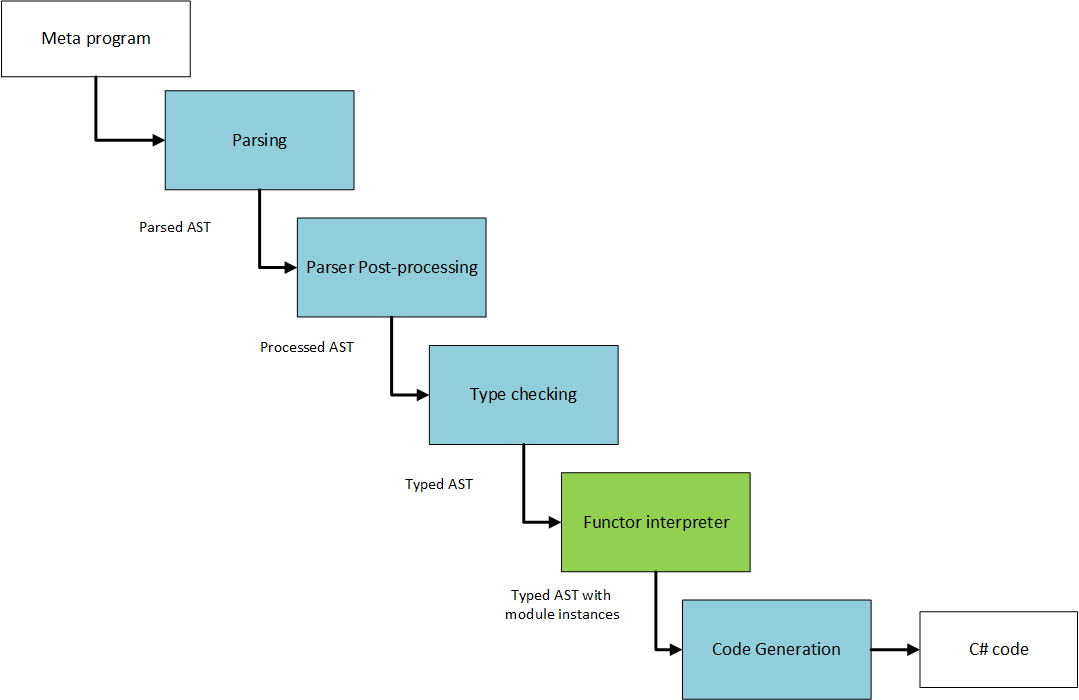
\includegraphics[width=\textwidth]{Figures/chapter_functors/compiler_architecture_functors}
	\caption{Compiler architecture with functor interpreter}
	\label{fig:ch_functors_compiler_architecture}
\end{figure}

\begin{figure}
	\centering
	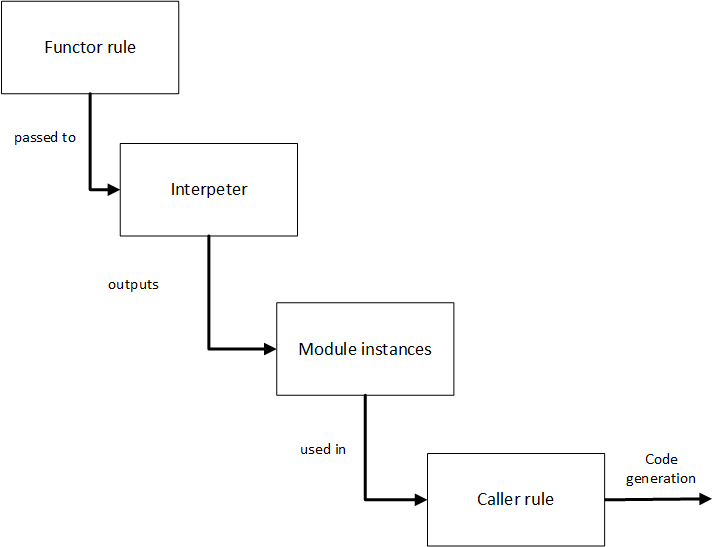
\includegraphics[width=\textwidth]{Figures/chapter_functors/functor_rule_processing}
	\caption{Functor processing}
	\label{fig:ch_functors_functor_processing}
\end{figure}

\section{Record implementation with modules}
\label{sec:ch_functors_record_implementation}
In Section \ref{subsec:ch_functors_inlining} we showed how Casanova entities can be expressed, at meta-language level, as a tuple of field names and values. We also showed that getters and setters always perform the same steps when looking up for the same field because the entity structure does not change at runtime. In this section we proceed to give an functor-based implementation of Casanova entities. We refer to this implementation as ``Record'', since a Casanova entity is simply a record from the point of view of the data representation. Moreover, since this solution works in general for any data structure that is isomorphic to a record. From now on we also use, as example, the physical body entity described in Section \ref{subsec:ch_functors_casanova_example}.

A module for records simply contains a functor that returns the type of the record. This functor, in general, can return any type since the type of the record can be ``customized'' and depends on the specific definition given by the programmer (thus it cannot be known beforehand). For this reason we use \textit{kind} as return type for this functor. The functor itself is parameterless since nothing is required to generate the type of a record.

\begin{lstlisting}
Module "Record" : Record {
  Functor "RecordType" : * }
\end{lstlisting}

The data representation of the record will be a tuple as shown in Section \ref{subsec:ch_functors_inlining}. For this purpose, we need two functors that are able to represent the type of a record in a recursive way with one being the type of an empty record (a record with no fields) and another a record field followed by the rest of the record representation. The functor for the empty record simply returns the type of the record module, while the functor to represent a record field takes as input a \texttt{string}, representing the name of the field, \textit{kind} because a record field can have any type, and a \texttt{Record} which represents all the other fields coming after the current one. 

\begin{lstlisting}
Functor "EmptyRecord" : Record
Functor "RecordField" => string => * => Record : Record
\end{lstlisting}

After declaring the functors necessary to build a record, we proceed to define their implementation in the form of rules. The functor for an empty record simply generates a module containing a function \texttt{cons}, that is the constructor for the record, that simply returns unit (because an empty record does not contain any field). Consistently, the functor \texttt{RecordType} implemented by the module will simply return \texttt{unit} as type. Note that a module instantiation must implement \textbf{at least} all the declarations of the module (like for an interface), but can add other declarations and implementations that are not shared by all the module instantiations. For example \texttt{cons} for an empty record is different than the one for a non-empty one.

\begin{lstlisting}
-------------------
EmptyRecord => Record {

  Func "cons" : unit
  
  ------------------
  RecordType => unit
  
  ------------------
  cons -> ()

}
\end{lstlisting}

A record field must be constructed through a functor that takes the field name, the type of the field, and the type of the rest of the record. This functor will construct the type of a record as a \texttt{Tuple}, where the first element is the type of the current field and the second the type of the rest of the record. The constructor of the record field will be a function that takes as input an argument of the type of the current field, a tuple representing the remaining part of the record and returns a tuple combining the current field and the rest of the record.

\begin{lstlisting}
------------------
RecordField name type r = Record {
  Func "cons" -> type -> r.RecordType : RecordType

  ---------------------------------------
  RecordType => Tuple[type,r.RecordType]

  -------------------
  cons x xs -> (x,xs)}
\end{lstlisting}

Consider now the physical body representation given above. We show how to use the functors we have just defined to build an instance of a physical body. First of all we defined a functor \texttt{PhysicalBodyType} that returns a \texttt{Record}.

\begin{lstlisting}
Functor "PhysicalBodyType" : Record
\end{lstlisting}

The final representation of the type that should be returned by\\ \texttt{PhysicalBodyType} is \texttt{Tuple[Vector2,Tuple[Vector2,unit]]} because the field\\ \texttt{Position} and \texttt{Velocity} have type \texttt{Vector2}. Note that \texttt{Vector2} can be trivially implemented in Metacasanova as a tuple containing two floating point values. Here we use this type assuming that has already been defined above. The same applies to \texttt{unit}, which can be defined as a meta-data with no arguments.

The rule to evaluate \texttt{PhysicalBodyType} will call in its premises\\ \texttt{EmptyRecord} and \texttt{RecordField} to generate the type of the tuple appropriately:

\begin{lstlisting}
EmptyRecord => empty
RecordField "Velocity" Vector2 empty => velocity
RecordField "Position" Vector2 velocity => body
----------------------------
PhysicalBodyType => body
\end{lstlisting}

Let us now analyse in detail what the premises generate: the first premise will generate an instance of \texttt{EmptyRecord} and bind it to the variable \texttt{empty}. The instance of this module is parameterless and thus will always be the same every time the functor is invoked. The second premise will instantiate \texttt{RecordField} by using the string \texttt{"Velocity"} as field name, \texttt{Vector2} as field type, and \texttt{empty} as argument for the remaining part of the record (there is no other field after \texttt{Velocity} in the physical body). The instantiation of \texttt{RecordField} produces a rule for the functor \texttt{RecordType}. According to the definition above this functor generates \texttt{Tuple[type,r.RecordType]}. By replacing the argument values provided in the premise, we have 

\begin{lstlisting}
type := Vector2
r := empty := EmptyRecord
\end{lstlisting}

\noindent
Thus \texttt{r.RecordType} uses the functor \texttt{RecordType} in the instance of\\ \texttt{EmptyRecord} which returns the type \texttt{unit} (the call can be seen as\\ \texttt{empty.RecordType}). Thus \texttt{r.RecordType} can be replaced with \texttt{unit}, thus leading to \texttt{Tuple[Vector2, unit]}. Thus the rule for the functor \texttt{RecordType} generated in the module returned by the second premise will be:

\begin{lstlisting}
-----------------------
RecordType => Tuple[Vector2,unit]
\end{lstlisting}

By replacing the argument variables with the values provided in the second premises we can also get the declaration and rule for \texttt{cons}. By replacing again \texttt{type} and \texttt{r.RecordType} as done before, we have that the declaration for \texttt{cons} in the current instance of the module becomes:

\begin{lstlisting}
Func "cons" -> Vector2 -> unit: Tuple[Vector2,unit]
\end{lstlisting}

\noindent
while the corresponding rule will be generated as

\begin{lstlisting}
--------------------
cons x xs -> (x,xs)
\end{lstlisting}

\noindent
The complete module instance will then look like:

\begin{lstlisting}
velocity := Record {
  Func "cons" -> Vector2 -> unit: Tuple[Vector2,unit]
  
  -----------------------
  RecordType => Tuple[Vector2,unit]
  
  --------------------
  cons x xs -> (x,xs)
}
\end{lstlisting}

The third premise calls \texttt{RecordField} with 

\begin{lstlisting}
name := "Position"
type := Vector2
r := velocity
\end{lstlisting}

\noindent
Now in the definition of the \texttt{RecordField} module again the functor\\ \texttt{RecordType} returns \texttt{Tuple[type,r.RecordType]}. Now \texttt{r.RecordType} can be rewritten as \texttt{velocity.RecordType} that returns (see the instantiation of \texttt{velocity} above) \texttt{Tuple[Vector2,unit]}. Thus \texttt{RecordType} for the field \texttt{Position} will be instantiated as

\begin{lstlisting}
-----------------------
RecordType => Tuple[Vector2,Tuple[Vector2,unit]]
\end{lstlisting}

\noindent
Analogously the declaration of \texttt{cons} will be instantiated as

\begin{lstlisting}
Func "cons" -> Vector2 -> Tuple[Vector2,unit]: Tuple[Vector2,Tuple[Vector2,unit]]
\end{lstlisting}

\noindent
while its rule is the same of the second premise. The full module instance will then be

\begin{lstlisting}
body := Record {
  Func "cons" -> Vector2 -> Tuple[Vector2,unit]: Tuple[Vector2,Tuple[Vector2,unit]]
  
  -----------------------
  RecordType => Tuple[Vector2,Tuple[Vector2,unit]
  
  --------------------
  cons x xs -> (x,xs)
}
\end{lstlisting}

\noindent
which is returned by the functor \texttt{PhysicalBodyType}. In order to build an instance of the physical body, we define a function that returns a value of type \texttt{PhysicalBodyType}. which in turn is simply \texttt{Tuple[Vector2,\\Tuple[Vector2,unit]}):

\begin{lstlisting}
Func "PhysicalBody" : PhysicalBodyType.RecordType

-----------------------
PhysicalBody -> PhysicalBodyType.cons((10.0,10.0),((10.0,0.0),()))
\end{lstlisting}

\noindent
The rule creates a physical body in position $(10,10)$ moving at velocity $(10,0)$.\\

One of the main arguments in favour of using functors was that they should allow to embed the type system of the embedded language in the meta-type system of Metacasanova. This means that, at compile time, the meta-compiler should be able to detect a physical body that is constructed in the wrong way. Let us then assume that we define another function to build a physical body where the programmer uses a scalar for the velocity instead of a vector:

\begin{lstlisting}
Func "WrongPhysicalBody" : PhysicalBodyType.RecordType

-------------------------------------
WrongPhysicalBody ->  PhysicalBodyType.cons((10.0,10.0),(10.0,()))
\end{lstlisting}

\noindent
What happens is that \texttt{PhysicalBodyType.RecordType} is equal to\\ \texttt{Tuple[Vector2,Tuple[Vector2,unit]]}. At this point the type checker of Metacasanova will successfully match the first element of the tuple returned by the rule, which is correctly provided as a value of type \texttt{Vector2}, but will fail to check the second, which is \texttt{double} where it expects a \texttt{Vector2}. This check happens statically, rather than dynamically at runtime as was the case with the implementation based on dictionaries in Section \ref{subsec:ch_mcnv_languages_casanova_semantics}.

\section{Getting Values from Record Fields}
\label{sec:ch_functors_record_getter}
Getting a value from a record field requires defining a module \texttt{Getter} containing a functor \texttt{GetField} that returns the type of the field that we need to get. This type will be used as the return type of the function \texttt{get} that is able to get that specific field. This function is also contained in this module and takes as argument the record from which we are getting the value and returns, as said above, the value of the field. The module \texttt{Getter} is built using the name of the field that is able to read and the record to read from.

\begin{lstlisting}
Module "Getter" => (name : string) => (r : Record) : Getter { ... }
\end{lstlisting}

The functor \texttt{GetType} returns kind because in general the type of the field of a record is arbitrary. The function \texttt{get} uses in its declaration the functor \texttt{RecordType} to determine the type of the record to use and \texttt{GetType} to determine the type of the field to read. The complete module will look like

\begin{lstlisting}
Module "Getter" => (name : string) => (r : Record) : Getter {
  Functor "GetType" : *
  Func "get" -> (r.RecordType) : GetType
}
\end{lstlisting}

\noindent
The getter has two implementations of the rule that instantiates the \texttt{Getter} module: one is used when the current field in the module tuple is the one we are trying to read, and the other that is able to build the correct getter if the field is in the remaining part of the record. The first happens when the name of the current field is the same as the field name provided as argument of the functor \texttt{GetField}. In this case we have the following rule for the functor:

\begin{lstlisting}
Functor "GetField" => string => Record : Getter
\end{lstlisting}

\begin{lstlisting}[caption = Getting a field (case 1),label = lst:ch_functors_getter1]
name = fieldName
thisRecord := RecordField name type r
--------------------------------------
GetField fieldName (RecordField name type r) => Getter fieldName thisRecord {
  
  ---------------
  GetType => type
  
  ---------------
  get (x,xs) -> x
}
\end{lstlisting}

\noindent
The functor \texttt{GetType} simply returns the type of the current record field, because it is the correct field to read, and \texttt{get} returns the first element of the record tuple, which represents the value stored in the field itself.

When the field we are trying to read is not the one we are currently examining in the record tuple, we must build a getter functor that is able to recursively get the field from the remaining part of the record. At this purpose, we have to extend the \texttt{Getter} with an additional functor \texttt{GetAnotherField} that returns a module instance capable of reading the value from the correct field in the remaining part of the record and its type. The implementation of the rule for this case is the following:

\begin{lstlisting}[caption = Getting a field (case 2),label = lst:ch_functors_getter2]
name <> fieldName
thisRecord := RecordField name type r
-------------------------------------
GetField fieldName (RecordField name type r) => Getter fieldName type thisRecord {
		Functor "GetAnotherField" : Getter
		
		GetField fieldName r => otherGetter
		------------------------------
		GetAnotherField => otherGetter
		
		GetAnotherField => g
		---------------------
		GetType => g.GetType
		
		GetAnotherField => getter
		getter.get xs -> v
		------------------
		get (x,xs) -> v
  }
}
\end{lstlisting}

\noindent
The rule for the functor \texttt{GetAnotherField} simply calls recursively the rule for \texttt{GetField} with the remaining part of the record. If the next field is the correct one then this time we will use the rule in Listing \ref{lst:ch_functors_getter1}, otherwise the rule in Listing \ref{lst:ch_functors_getter2} will be re-applied until the correct field is reached. The functor \texttt{GetType} simply calls \texttt{GetAnotherField} to obtain the module instance necessary to get the field from the rest of the record, and then calls the functor \texttt{GetType} from that instance. Finally, the function \texttt{get} will again use \texttt{GetAnotherField} and then call the \texttt{get} function from the getter returned by \texttt{GetAnotherField} with the remaining part of the record tuple. This function call will return the desired value that will be used also as result of the current \texttt{get}.

Let us now consider again the physical body implemented with functors in Section \ref{sec:ch_functors_record_implementation} and let us assume that we want to get the value of the field \texttt{Position}. We define a function \texttt{getPos} that takes as input a physical body and returns \texttt{Vector2}. This function will use \texttt{GetField} in its premises to generate the getter for \texttt{Position} and will then call the \texttt{get} function from the generated module instance.

\begin{lstlisting}[caption = Getter for the Position field, label = lst:ch_functors_position_getter]
Func "getPos" : Vector2

GetField "Position" PhysicalBodyType => getter
PhysicalBody -> body
getter.get body -> p
-----------------
getPos -> p
\end{lstlisting}

\noindent
Note that in the code above we are using the functor \texttt{PhysicalBodyType} and the function \texttt{PhysicalBody} defined in Section \ref{sec:ch_functors_record_implementation}. Now let us analyse step-by-step what happens when we call \texttt{getPos}. The first premise will call the functor \texttt{GetField} with 

\begin{lstlisting}
fieldName := "Position"
r := PhysicalBodyType := RecordField "Position" Vector2 (RecordField "Velocity" Vector2 EmptyRecord)
\end{lstlisting}

\noindent
At this point the rule for \texttt{GetField} will deconstruct \texttt{RecordField} in its conclusion by means of pattern matching and set 

\begin{lstlisting}
name := "Position"
type := Vector2
r := RecordField "Velocity" Vector2 EmptyRecord
\end{lstlisting}
 
\noindent
Since \texttt{name} = \texttt{fieldName} we fall in the case in Listing \ref{lst:ch_functors_getter1}. Thus we instantiate the module \texttt{Getter} by setting the construction arguments to 

\begin{lstlisting}
name := "Position"
r := RecordField "Position" Vector2 (RecordField "Velocity" Vector2 EmptyRecord)
\end{lstlisting}

\noindent
In this module instance the functor \texttt{GetType} returns \texttt{type :=  Vector2} and \texttt{get} returns the first element of the record tuple. At this point, the third premise will call \texttt{get} from this module instance by passing the record tuple\\ \texttt{((10.0,10.0),((10.0,0.0),()))}, which in turn returns correctly \texttt{(10.0,10.0)}.

Now let us assume that we want to retrieve the value of "Velocity" instead. We define an analogous function \texttt{getVel} as follows

\begin{lstlisting}
Func "getVel" : Vector2

GetField "Velocity" PhysicalBodyType => getter
PhysicalBody -> body
getter.get body -> v
-----------------
getVel -> v
\end{lstlisting}

\noindent
This time the functor \texttt{GetField} is called with

\begin{lstlisting}
fieldName := "Velocity"
r := PhysicalBodyType := RecordField "Position" Vector2 (RecordField "Velocity" Vector2 EmptyRecord)
\end{lstlisting}

\noindent
thus the rule in case 2 is triggered. This rule will generate an instance of \texttt{Getter}

\begin{lstlisting}
fieldName := "Velocity"
type := Vector2
r := RecordField "Velocity" Vector2 EmptyRecord
\end{lstlisting}

\noindent
This rule will generate a module containing the auxiliary functor \texttt{GetAnotherField} that is capable to retrieve the correct field in the remaining part of the record. The rule that processes \texttt{GetAnotherField} will call, in its premise, \texttt{GetField} with

\begin{lstlisting}
fieldName := "Velocity"
r := RecordField "Velocity" Vector2 EmptyRecord
\end{lstlisting}

Since now the name of the field of the getter coincides with the name of the field in \texttt{RecordField}, this premise will now trigger the rule in Listing \ref{lst:ch_functors_getter2} that in turn generates an instance of \texttt{GetField} containing the following:

\begin{lstlisting}[caption = Getter for Velocity generated by \texttt{GetAnotherField}, label = lst:ch_functors_velocity_getter2]
Func "get" -> Tuple[Vector2,unit] : Vector2

-------------------
GetType => Vector2


----------------
get (x,xs) -> x
\end{lstlisting}

\noindent
This module instance will be the one returned by the rule of \texttt{GetAnotherField}. The rule of the functor \texttt{GetType} for \texttt{Velocity} will use \texttt{GetAnotherField} to retrieve the correct field type using the module instance generated in Listing \ref{lst:ch_functors_velocity_getter2} and return it (which is \texttt{Vector2}). The rule for the function \texttt{get} will use \texttt{GetAnotherField} to call the the \texttt{get} function from Listing \ref{lst:ch_functors_velocity_getter2} passing the second element of the record tuple as argument and returns the result of this function call.

Note that the module instantiation will be again performed at compile time, thus the only operations performed at runtime are the calls to the \texttt{get} functions contained in the module instantiations.

\section{Setting Values of Record Fields}
\label{sec:ch_functors_record_setter}
The setter module is analogous to the getter, except that this time the module must generate a function that, in addition to the record, takes as input the value to write in the field. This function returns a modified copy of the record tuple where the value associated to the field has been changed. For this purpose we need a module containing a functor \texttt{SetType} that returns the type of the field to set. This functor will be used to build the declaration of a function \texttt{set} that is able to set the specified field.

\begin{lstlisting}
Module "Setter" => (name : string) => (r : Record) : Setter {
	Functor "SetType" : *
	Func "set" -> r.RecordType -> SetType : r.RecordType
}
\end{lstlisting}

\noindent
The declaration of the function \texttt{set} uses \texttt{r.RecordType} to define the type of the record argument, \texttt{SetType} to define the type of the field to set, necessary for the argument containing the value to set, and returns \texttt{r.RecordType}, which is the modified version of the record.

Analogously to the getter, we need a functor that instantiates \texttt{Setter} and has two different implementations of the instantiation rule: one where the field of the current element of the record tuple coincides with the one we want to set, and the other where the field is different and that is able to build a setter for the remaining part of the record tuple.

\begin{lstlisting}
Functor "SetField" => string => Record : Setter
\end{lstlisting}

The first case is implemented as follows:

\begin{lstlisting}[caption = Setting a field (case 1), label = lst:ch_functors_setter1]
name = fieldName
thisRecord := RecordField name type r
------------------------------
SetField fieldName (RecordField name type r) => Setter fieldName thisRecord {

  ----------------
  SetType => type
  
  ----------------------
  set (x,xs) v -> (v,xs)
}
\end{lstlisting}

\noindent
The function \texttt{SetType} simply returns the type of the field in the current \texttt{RecordField}, while the rule for \texttt{set} replaces the first value in the record tuple with the new value. The second rule is implemented as follows

\begin{lstlisting}[caption = Setting a field (case 2), label = lst:ch_functors_setter2]
name <> fieldName
thisRecord := RecordField name type r
-------------------------------------
SetField fieldName (RecordField name type r) => Setter fieldName thisRecord {
  Functor "SetAnotherField" : Setter
  
  SetField fieldName r => setter
  -------------------------------
  SetAnotherField => setter
  
  SetAnotherField => s
  -------------------------
  SetType => s.SetType
  
  SetAnotherField => setter
  setter.set xs v -> xs'
  ----------------------
  set (x,xs) v -> (x,xs')
}
\end{lstlisting}

\noindent
The functor \texttt{SetAnotherField} is an auxiliary functor that recursively calls\\ \texttt{SetField} with the remaining part of the record. Eventually \texttt{SetField} will trigger the rule in Listing \ref{lst:ch_functors_setter1} when the correct field is encountered. This auxiliary functor is then used in \texttt{SetType} to retrieve the correct type of the record field and in the function \texttt{set} to call the correct \texttt{set} function for the field. The \texttt{set} function in the setter generated by \texttt{SetAnotherField} returns a modified version of the record that is replaced in the tuple.

Let us now consider again the physical body and assume that we want to define a setter for \texttt{Position}. Again we define a function \texttt{setPos} for the field:

\begin{lstlisting}
Func "setPos" -> Vector2 : PhysicalBodyType

SetField "Position" PhysicalBodyType => setter
PhysicalBody -> body
setter.set body -> body'
-----------------------
setPos v -> body'
\end{lstlisting}

\noindent
Again we are using the functor \texttt{PhysicalBodyType} and the function\\ \texttt{PhysicalBody} defined in Section \ref{sec:ch_functors_record_implementation}. The first premise of this rule will call \texttt{SetField} with

\begin{lstlisting}
fieldName := "Position"
name := "Position"
type := Vector2
r := RecordField "Velocity" Vector2 EmptyRecord
\end{lstlisting}

\noindent
which, in turn, instantiates \texttt{Setter} with 

\begin{lstlisting}
name := "Position"
r := RecordField "Position" Vector2 (RecordField "Velocity" Vector2 EmptyRecord)
\end{lstlisting}

\noindent
In this module instance \texttt{r.RecordType} will be\\ \texttt{Tuple[Vector2,Tuple[Vector2,unit]]} and \texttt{SetType} returns \texttt{Vector2}. The whole instance will look like

\begin{lstlisting}
Func "set" -> Tuple[Vector2,Tuple[Vector2,unit]] -> Vector2 : Tuple[Vector2,Tupe[Vector2,unit]]

------------------
SetType => Vector2


----------------------
set (x,xs) v -> (v,xs)
\end{lstlisting}

\noindent
Now let us assume that we want to build a setter for \texttt{Velocity}. We have to define a function \texttt{setVel} as follows

\begin{lstlisting}
Func "setVel" -> Vector2 : PhysicalBodyType

SetField "Velocity" PhysicalBodyType => setter
PhysicalBody -> body
setter.set v -> body'
-------------------------
setVel v -> body'
\end{lstlisting}

\noindent
The first premise of this rule will now invoke \texttt{SetField} with

\begin{lstlisting}
fieldName := "Velocity"
name := "Position"
type := Vector2
r := RecordField "Velocity" Vector2 EmptyRecord
\end{lstlisting}

\noindent
which will trigger the rule in Listing \ref{lst:ch_functors_setter2} instead. This will create an instance of \texttt{Setter} containing  the auxiliary functor \texttt{SetAnotherField}. The rule for this functor will call in turn \texttt{SetField} with

\begin{lstlisting}
fieldName := "Velocity"
name := "Velocity"
type := Vector2
r := EmptyRecord
\end{lstlisting}

\noindent
that will generate a different instance of \texttt{Setter}, this time using the rule in Listing \ref{lst:ch_functors_setter1}. The auxiliary setter will contain a functor \texttt{SetType} returning \texttt{Vector2} and a function \texttt{set} that inserts the value for \texttt{Velocity} in the record tuple. The \texttt{set} in the auxiliary setter will be used in the setter of \texttt{Velocity} to obtain the modified copy of the record containing the new value. Again all the modules are generated at compile time, thus the only operations performed at runtime are the calls to the \texttt{set} functions of the field setter and eventual auxiliary modules.

\section{Handling errors in getters and setters}
\label{sec:ch_functors_error_handling}
In Section \ref{sec:ch_functors_record_getter} and \ref{sec:ch_functors_record_setter} we explained how to use functors to implement getters and setters for the fields of a record. The explanation however did not take into account possible mistakes that could be committed during the definition of setters and getters for a specific record.

A possible mistake that could arise in the process of defining getters and setters would be to provide an incompatible type for the \texttt{get} function of a field. For instance, let us assume that we define \texttt{getPos} as

\begin{lstlisting}
Func "wrongGetPos" : double

GetField "Position" PhysicalBodyType => getter
PhysicalBody -> body
getter.get body -> v
-----------------
wrongGetPos -> v
\end{lstlisting}

\noindent
As explained above the getter module will contain a function \texttt{get} that returns a \texttt{Vector2}, because that is the type of the field \texttt{Position}. In the process of building the module, this type is automatically retrieved from the definition of \texttt{PhysicalBodyType}. At this point the meta-compiler would report an error message because this wrong definition of \texttt{getPos} returns \texttt{double} but \texttt{get} returns a \texttt{Vector2}. Note that, as previously explained in Section \ref{sec:ch_functors_record_implementation}, this is possible because functors are able to embed the type system of the embedded language into the Metacasanova type system.


Another possible mistake is accessing a field that is not defined for the record. For instance, let us assume that someone tries to build a getter for a field that does not exist in physical body, namely a field \texttt{Acceleration}. As usual we would define a function for the getter such as

\begin{lstlisting}
Func "getAcc" : Vector2

GetField "Acceleration" PhysicalBodyType => getter
PhysicalBody -> body
getter.get body -> v
---------------
getAcc -> v
\end{lstlisting}

\noindent
The first premise of this rule will call the functor \texttt{GetField} with

\begin{lstlisting}
fieldName := "Acceleration"
name := "Position"
type := Vector2
r := RecordField "Velocity" Vector2 EmptyRecord
\end{lstlisting}

\noindent
As seen above, this rule will generate an auxiliary module by recursively call \texttt{GetField} with

\begin{lstlisting}
fieldName := "Acceleration"
name := "Velocity"
type := Vector2
r : = EmptyRecord
\end{lstlisting}

\noindent
but at this point, since again \texttt{fieldName} $\neq$ \texttt{name} we will recursively call \texttt{GetField}. At this point we will fail to run a suitable rule for the functor, since the only two versions we have so far are able to process \texttt{RecordField} and not \texttt{EmptyRecord}, thus the pattern matching in the conclusion would fail. The meta-compiler will in any case fail to generate code, since the functor evaluation will fail and thus the whole code generation, but this approach is not ``clean'', since the meta-compiler will report a generic error regarding the rule execution failure. An alternative to this, is to include a case for the rule that processes \texttt{EmptyRecord}. A getter for an \texttt{EmptyRecord} returns \texttt{()} and \texttt{GetType} returns the type \texttt{unit}. This rule can be implemented as follows:

\begin{lstlisting}

fieldName <> name
thisRecord := RecordField name type EmptyRecord
-------------------------------
GetField fieldName (RecordField name type EmptyRecord) => Getter fieldName thisRecord {
	
  ----------------
  GetType => unit
  
  ----------------
  get (x,xs) -> ()
}
\end{lstlisting}

In this way the first premise of the rule of \texttt{getAcc} would generate a getter that takes a physical body and returns \texttt{unit}. When the rule calls this getter and returns \texttt{unit}, this will be incompatible with the return type of \texttt{getAcc} that should be a \texttt{Vector2}. The same can be done for \texttt{setAcc}, that is we extend the rule for \texttt{SetField} with an additional case:

\begin{lstlisting}
fieldName <> name
thisRecord := RecordField name type EmptyRecord
--------------------------
SetField fieldName (RecordField name type EmptyRecord) => Setter fieldName thisRecord {
	
	----------------
	SetType => unit
	
	----------------------
	set (x,xs) v -> (x,xs)
}
\end{lstlisting}

\noindent
In this way, when invoking \texttt{set} in the premise \texttt{setAcc} the compiler will signal a type error because at some point it will try to use the \texttt{set} for the \texttt{EmptyRecord} with \texttt{Vector2}. Another alternative, which goes beyond the scope of this chapter, would be to allow rules in meta-casanova to output custom compilation errors. In this way we could write the very same rule case done above but this time we would return a compilation error message reporting that the field does not exist.

\section{Evaluation}
\label{sec:ch_functors_evaluation}
In the previous sections we presented an extension to the meta-language of Metacasanova that allows to embed the type system of an embedded language, whose definition is implemented in Metacasanova, in the meta-type system of Metacasanova. We claimed that this would improve the runtime performance of a program written in the embedded language because we could get rid of all the dynamic checks and accesses to meta-data structures used to implement data structures in the embedded language, such as records. In this section we present the experimental evaluation that should produce the evidence to back up this claim. We proceed to describe the experimental set-up and then we comment the results.

\subsection{Experimental Set-up}
In this experiment we use the implementation of records with functors described in this chapter and we compare its runtime performance with its dynamic counter part, i.e. the implementation that uses dictionaries, that was used to implement the Casanova memory model in Section \ref{subsec:ch_mcnv_languages_casanova_semantics}. The sample measures the run-time of both the functor implementation and the implementation with dynamic tables. We run the test by varying both the number of record instances and the number of fields per record. The test is run with a sample of 10000, 100000, and 1000000 record instances and with a number of fields from 1 to 10. We neglect to consider different field types, as the performance of look-up operations is not affected by the type of the fields themselves.

\subsection{Results}

In Table \ref{tab:ch_functors_results}, we can see that the optimization using Functors leads to a performance increase on average of about 11 times, with peaks of 30 times. The gain increases with the number of fields, thus the implementation with functors is particularly effective for records with high number of fields. This is due to the fact that the runtime complexity of a dynamic table depends on the number of entries stored in it (which would be the fields in our case) and thus, when the fields are few, this number is very close to the complexity of the functorial implementation, which is constant. When the number of fields increases, the performance of the functorial implementation remains the same while the dynamic table one worsens visibly. The constant complexity of the functorial implementation is due to the fact that the meta-compiler builds the functions of a getter or setter module instance, used to look up a specific field or set its value, at compile time by generating the appropriate module instances with the functors. The \texttt{get} and \texttt{set} functions described above can either immediately get or set the value of the field and return the result of this operation, or call the getter or setter of an auxiliary module instance that is able to read or write the appropriate field. The only overhead is the overhead of chaining calls to Metacasanova functions, thus the overhead of creating and executing the code that implements the rule behaviour described in Section \ref{sec:ch_metacasanova_code_generation}.

Figure \ref{fig:ch_functors_chart} shows a chart of the overall performance of the two techniques (the data points are taken from Table \ref{tab:ch_functors_results}). The horizontal axis contains the number of fields per record, while the vertical axis contains the number of records that are being updated. We can see that the performance of the dynamic table degrades considerably when increasing the number of fields, and that the higher the number of records is, the steeper the curve is. On the other hand, the performance of the implementation with functors is almost constant, regardless of the number of fields or records that are being updated. Moreover, note that the performance of the dynamic table is improved by the fact that we are using a dictionary implemented in .NET. If the symbol table were represented as a meta-data structure in the language, the performance would be even worse, since it would have to be encoded as a list of pairs with the field name and its value, and its manipulation would be affected by the evaluation rules that should implement this behaviour. Furthermore, the dynamic lookup should be done also to ensure that the types of the record fields are used consistently (which is not accounted for here, for example to prevent that a record is constructed with incompatible values for its fields), while this check is done at compile time with functors, thus drastically improving the performance.

\subsubsection{Dynamic Table implementation Choice}
After both these considerations and those presented in Chapter \ref{sec:ch_mcnv_languages_evaluation} a legitimate doubt could be uttered about the choice of the implementation of the dynamic tables. We mentioned multiple times that we chose to use a tree-based implementation of the dictionary, but a valid objection could be that one could use a HashTable whose complexity is $O(1)$. This assumption cannot be applied to this case for the following reasons:

\begin{itemize}
\item The hash table access operations have a complexity of $O(1)$ when the number of entries stored in it is very big. Indeed the definition of big-oh states that $f(n) = O(g(n))$ if
\begin{align*}
\exists c \in \mathbb{R}: \lim_{n \to \infty}\dfrac{f(n)}{g(n)} = c
\end{align*}
\noindent
thus it makes sense to talk in term of complexity only if the size of the table is very large. It is very unlikely that a record will contain a large number of fields. In this scenario, the performance of a hash table decays because the running time is affected by the computation of the hash function for every access and the resize of the table performed to decrease the load factor in order to minimize the number of collisions \cite{cormen2001introduction}. In the case of records, where the amount of fields and thus of entries in the table is limited, the performance of the tree implementation and the hash table are on the same order of magnitude.
\item  Metacasanova is a referentially transparent language, as all data structures are immutable. Referential transparency is a desirable property to have because it helps in the verification of the correctness of programs \cite{linger1988case, trammell1996incremental} and prevents side-effects. Hash tables have high performance only when mutability is allowed, but implementing an immutable hash table requires to recreate the whole table inserting all the entries again by re-hashing them. This does not happen in trees, where we do not need to recreate the whole tree but only the sub-tree that is affected by the manipulation of the data structure.
\end{itemize}

\begin{table}
	\centering
	\begin{tabular}{|c|c|c|c|}
		\hline
		\textbf{FIELDS}& \textbf{Functors (ms)}&\textbf{Dynamic Table (ms)} & \textbf{Gain}\\ \hline
		1&	1.00E-05&	5.00E-06&	0.50\\ \hline
		2&	9.00E-06&	1.30E-05&	1.44\\ \hline
		3&	9.00E-06&	2.70E-05&	3.00\\ \hline
		4&	9.00E-06&	4.50E-05&	5.00\\ \hline
		5&	9.00E-06&	7.00E-05&	7.78\\ \hline
		6&	9.00E-06&	9.90E-05&	11.00\\ \hline
		7&	9.00E-06&	1.33E-04&	14.78\\ \hline
		8&	9.00E-06&	1.75E-04&	19.44\\ \hline
		9&	9.00E-06&	2.20E-04&	24.44\\ \hline
		10&	9.00E-06&	2.70E-04&	30.00\\ \hline
		\multicolumn{2}{c|}{} & \textbf{Average gain} & 11.74\\ \cline{3-4}			
	\end{tabular}
	
	\vspace{0.15cm}
	\begin{tabular}{|c|c|c|c|}
		\hline
		\textbf{FIELDS}& \textbf{Functors (ms)}&\textbf{Dynamic Table (ms)} & \textbf{Gain}\\ \hline
		1&	9.60E-05&	6.30E-05&	0.66\\ \hline
		2&	9.40E-05&	1.59E-04&	1.69\\ \hline
		3&	9.50E-05&	3.04E-04&	3.20\\ \hline
		4&	9.60E-05&	5.03E-04&	5.24\\ \hline
		5&	9.60E-05&	7.52E-04&	7.83\\ \hline
		6&	9.60E-05&	1.05E-03&	10.95\\ \hline
		7&	9.70E-05&	1.41E-03&	14.57\\ \hline
		8&	9.80E-05&	1.82E-03&	18.59\\ \hline
		9&	9.90E-05&	2.29E-03&	23.17\\ \hline
		10&	1.00E-04&	2.81E-03&	28.05\\ \hline
		\multicolumn{2}{c|}{} & \textbf{Average gain} & 11.39\\ \cline{3-4}						
	\end{tabular}
	
	\vspace{0.15cm}
	\begin{tabular}{|c|c|c|c|}
		\hline
		\textbf{FIELDS}& \textbf{Functors (ms)}&\textbf{Dynamic Table (ms)} & \textbf{Gain}\\ \hline
		1&	9.47E-04&	7.29E-04&	0.77\\ \hline
		2&	9.51E-04&	1.78E-03&	1.87\\ \hline
		3&	9.50E-04&	3.33E-03&	3.51\\ \hline
		4&	9.60E-04&	5.43E-03&	5.66\\ \hline
		5&	9.65E-04&	8.03E-03&	8.32\\ \hline
		6&	9.71E-04&	1.11E-02&	11.44\\ \hline
		7&	9.75E-04&	1.47E-02&	15.12\\ \hline
		8&	9.82E-04&	1.89E-02&	19.28\\ \hline
		9&	9.92E-04&	2.37E-02&	23.86\\ \hline
		10&	1.00E-03&	2.87E-02&	28.62\\ \hline
		\multicolumn{2}{c|}{} & \textbf{Average gain} & 11.84\\ \cline{3-4}						
	\end{tabular}
 	\caption{Running time with the functor optimization and the dynamic table with 10000, 100000, and 1000000 records.}
	\label{tab:ch_functors_results}
\end{table}

\begin{figure}
	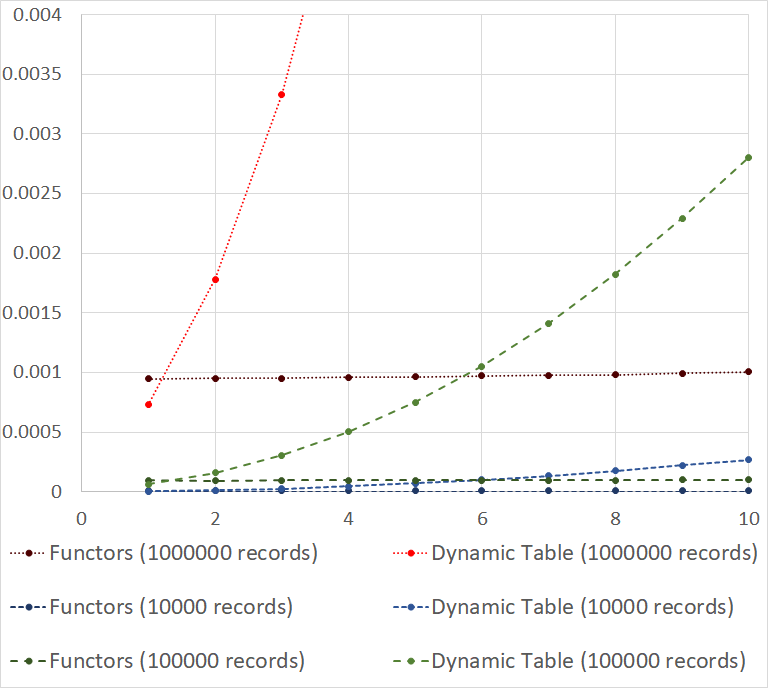
\includegraphics[width = \textwidth]{Figures/chapter_functors/functor_chart}
	\caption{Execution time of the different memory models}
	\label{fig:ch_functors_chart}
\end{figure}

\section{Summary}
In this chapter we addressed the problem described in Section \ref{sec:ch_mcnv_languages_evaluation} about the performance of the generated code and the forced dynamic behaviour of languages implemented in Metacasanova. We started by informally state that this issue was due to the fact that it was not possible to embed the type system of a language in the meta-type system of Metacasanova, and this caused all the dynamic lookups and accesses at runtime. This issue can be avoided by using a meta-language abstraction that allows both to define the type system of the embedded language in terms of the meta-type system of Metacasanova and to generate the code for the accesses to the data structures of the embedded language at compile time. For this purpose, we proposed a language extension that provides such abstraction in terms of modules and functors. We then proceeded to provide an example of their usage in the context of record getters and setters for their fields. We then measured the performance gain by comparing the implementation with functors with the one using dynamic tables that was employed for the Casanova language implementation shown in Section \ref{subsec:ch_mcnv_languages_casanova_semantics}. The results show that the performance of operations on records in the case of functors is up to 30 times faster than the dynamic table implementation. We have also shown that the performance of such operations in the case of functors is constant with respect to the number of fields to update, while the performance of the dynamic table drastically worsens when the number of fields in a record increases. In the next chapter we will show a further example of use of functors to re-implement Casanova semantics and extend the language with abstractions to express the networking behaviour for multiplayer games.

	
\chapter{Language Design with Functors}
\label{ch:functor_languages}
\epigraph{A monad is just a monoid in the category of endofunctors, what's the problem?}{James Iry}
In Section Chapter \ref{ch:languages} we showed an implementation in Metacasanova of Casanova, a domain-specific language for game development and we discussed about the reason of the poor performance of that implementation. In Chapter \ref{ch:functors} we extended Metacasanova with functors and modules to allow to embed the type system of an embedded  language \footnote{See the introduction of Chapter \ref{ch:functors} for a definition of this term} in the meta-compiler to overcome the problem of dynamic lookups at runtime. We then showed an implementation of records with modules and functors that significantly improved the performance of memory accesses, as shown in Section \ref{sec:ch_functors_evaluation}. In this chapter we show how this language extension can be used to improve the performance of the implementation in Metacasanova of the domain-specific language for game development Casanova. In what follows we start by describing how entities are updated in Casanova to make their dynamics evolve with respect to time. We then proceed to discuss how functors can be used to describe the semantics of entity updates in Casanova, and we further refine it to support the semantics of interruption of Casanova rules. We conclude with an evaluation about the performance gain achieved by using this implementation over the previous one presented in Chapter \ref{ch:languages}

\section{Casanova entity update}
\label{subsec:ch_networking_casanova_update}
In Section \ref{subsec:ch_mcnv_languages_casanova_semantics} we described the memory representation of a Casanova entity in Metacasanova and how the rules of an entity are updated. What was skipped for brevity was to describe how the system behind Casanova updates the entities of a Casanova program. As briefly described in Section \ref{sec:ch_mcnv_languages_casanova_language}, the structure of a program in Casanova is a tree, whose root is a special entity called \textit{World}. The world entity can contain fields that are instances of other entities as well, thus creating an additional level in the program tree. This is, of course, allowed also for regular entities, thus the height of the tree is arbitrary. Each entity might contain a set of rules that describe its dynamic behaviour with respect to time, thus they are updated by considering the time difference between the current and the previous update (\textit{frames}). Updating a rule is enforced by traversing the entity tree, thus when the field of an entity is an entity itself, the system will first update the entity instance contained in the field and then update the current entity. Casanova also natively supports lists and tuples as valid data types, and this requires to handle their update as well: a tuple or a list might themselves contain instances of entities that must be updated accordingly. In the case of a list of entities, we must run the update on each element, while in the case of a tuple we must examine each element and check whether it requires an update or not. This process is called \textit{update traversal} and might become very complex, as list and tuples can be combined together in infinite many ways, thus the process recursively calls the proper update depending on the type of the field.

At this purpose, let us consider a simulation consisting of an arbitrary amount of physical bodies, in the fashion of what was used in Section \ref{subsec:ch_functors_casanova_example}. The world entity will contain a list of physical bodies that are updated during the simulation. The Casanova code that described such a simulation is the following:

\begin{lstlisting}
worldEntity World {
	PhysicalBodies : [PhysicalBody]
}

entity PhysicalBody {
	Position				: Tuple<float,float>
	Velocity				: Tuple<float,float>
	Acceleration		: Tuple<float,float>
	
	rule Position = Position + Velocity * dt
	rule Velocity = Velocity + Acceleration * dt
}
\end{lstlisting}

\noindent
In this simulation, the update starts from \texttt{World}. This entity contains only one field, which is a list of physical bodies. Since \texttt{PhysicalBody} is an entity, the update must be run individually for each element of the list. The world contains no rules so after updating its only field we complete its update. At this point the update of each physical body examines each fields. All fields are represented as a point in a 2D space with a tuple containing two floating-point values. The update will examine each value of the tuple and find that they do not require any update (again because the only language abstractions that exhibit dynamic behaviours are entities). The update will then move on to run the rules that will update the content of \texttt{Position} and \texttt{Velocity}. The update process is sketched in Figure \ref{fig:ch_networking_simulation_update} and can thus be seen as a process that consists of the following steps:

\begin{enumerate}[noitemsep]
	\item An \textit{entity update} that traverses all the fields and rules of the entity and calls the appropriate updater.
	\item A \textit{field update} that updates (or not) the field depending on its type. The fields that will be updated have type \texttt{List}, \texttt{Tuple}, or \texttt{Entity}.
\end{enumerate}

\begin{figure}
	\centering
	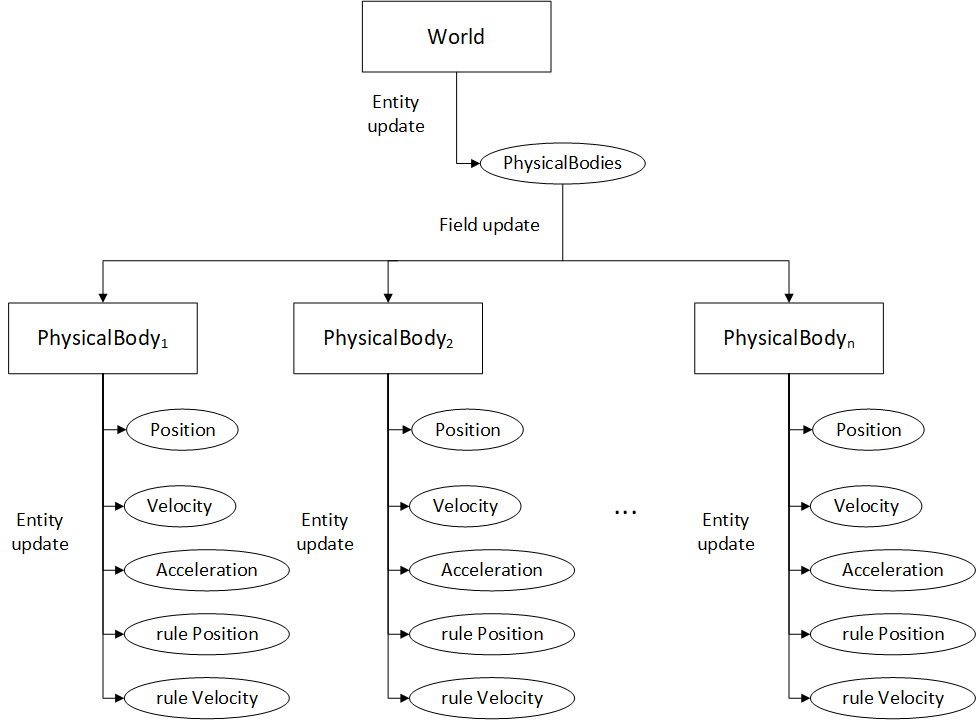
\includegraphics[width=\textwidth]{Figures/chapter_networking/update_traversal}
	\caption{Entity update for the simulation of physical bodies}
	\label{fig:ch_networking_simulation_update}
\end{figure}

\section{Update in Metacasanova}
\label{subsec:ch_networking_update_metacasanova}
The update mechanism described in Section \ref{subsec:ch_networking_casanova_update} can of course be integrated in the implementation of Casanova described in Chapter \ref{ch:languages}. In order to do so, we should dynamically look into the dictionary representing the entity fields at each update, extract the field and perform an update according to the following cases:

\begin{itemize}[noitemsep]
	\item If the field is a list, then we must examine each element and choose for each one whether it needs to be updated or not. This is done by recursively applying these cases (being a dynamic check we have to perform this check for each element).
	\item If the field is a tuple, then we behave as above.
	\item If the field is an entity, then we must run an update on it.
	\item In all the other cases the field is not updated.
\end{itemize}

\noindent
The cases above are translated into four rules in Metacasanova. The first three will use pattern-matching to decide whether the examined field is a list, a tuple, or an entity. The fourth one is a default rule that simply returns the field as it is. Moreover, each entity should store a list of rules that are updated as well, where all the get and set operations require dynamic lookups in the symbol table of the entity.

Repeating the traversal of the entity tree at each update at runtime is unnecessary since

\begin{itemize}[noitemsep]
	\item The structure of a Casanova entity cannot change at runtime. Its fields and field types will always remain the same.
	\item The fields affected by an entity rule and the rules of an entity do not change during the program execution.
\end{itemize}

\noindent
This means that, by exploiting modules and functors, we are able to specify the structure of the update at compile time and generate directly the function that performs the update at runtime, in the same fashion of what had been done for the record setter and getter. In the following sections we will describe extensively the implementation of the update using modules and functors in Metacasanova that generates at compile time the functions necessary to perform the update of a Casanova program. Note that we will refer to the implementation of records given in Section \ref{sec:ch_functors_record_implementation}.

\section{Updater Modules}
\label{subsec:ch_networking_updater_modules}
As explained above, Casanova needs to recursively update fields that are lists, tuples, or entity instances. At this purpose, we define a module that represents an \textit{updatable element} in the Casanova language. The module constructor takes as only argument the type of the element to update. This module contains a function \texttt{update} that is able to update a value of this particular type and uses an additional parameter \texttt{dt} that contains the time difference between the current and the previous update. The function returns the updated value of the element. It also contains an utility functor to return the type of the element.
 
\begin{lstlisting}
Module "ElementUpdater" => (elementType : *) : ElementUpdater {
	Functor "GetType" : *
	Func "update" -> elementType -> float : elementType
}
\end{lstlisting}

\noindent
The updater for a field is a module constructed by providing the record of the fields, its name as a string, and contains: (\textit{i}) an utility functor that returns the record used in the field updater, and (\textit{ii}) an update function that takes as input an instance of the record, \texttt{dt}, and returns the updated value of the field. We also define an external utility functor \texttt{GetFieldType} that can retrieve the type of a record field given the record it belongs to and its name. The rule for the functor calls the field getter and its \texttt{GetType} functor to retrieve the type of the field. This functor is used by the module constructor to correctly generate the return type of the \texttt{update} function.

\begin{lstlisting}
Functor "GetFieldType" => Record => string : *

GetField r name => getter
getter.GetType => type
---------------------------
GetFieldType r name => type

Module "FieldUpdater" => (r : Record) => (name : string) : FieldUpdater {
  Functor "GetRecord" : Record
  Func "update" -> r.RecordType -> float : (GetFieldType r name)
}
\end{lstlisting}

\noindent
Finally, the updater for a record is a module constructed by providing the record itself and contains: (\textit{i}) an utility functor that returns the type of the record, and (\textit{ii}) a function \texttt{update} that takes the instance of the record, \texttt{dt}, and returns an updated instance of the record.

\begin{lstlisting}
Module "RecordUpdater" => (r : Record) : RecordUpdater {
  Functor "RecordType" : *
  Func "update" -> r.RecordType -> float : r.RecordType
}
\end{lstlisting}

\section{Updatable elements}
\label{subsec:ch_networking_updatable_elements}
As explained above, the elements for which the update is needed can be lists, tuples, or entity instances. For this reason we have to create separately three different instances of the module \texttt{ElementUpdater} each one dedicated to updating one of those updatable elements. The first updatable element that we consider is an \textit{entity instance}. The module to update such updatable element uses a \texttt{RecordUpdater} to define how the entity instance should be updated. Indeed updating a field containing an entity instance requires to apply the specific record updater for that entity, which in turn returns the updated instance of the entity itself. Thus the declaration for the functor that constructs the proper instance of the module for the entity updater is the following:

\begin{lstlisting}
Functor "UpdateEntity" => RecordUpdater : ElementUpdater
\end{lstlisting}

\noindent
The rule for this functor extracts in its premise the type of the record by calling the utility functor \texttt{RecordType} in the record updater passed as parameter to \texttt{UpdateEntity}. The \texttt{update} function uses the record updater to recursively update the entity instance in its premise and then returns the result of this update.

\begin{lstlisting}
recordUpdater.RecordType => recordType
--------------------------
UpdateEntity recordUpdater => ElementUpdater recordType {

	----------------------
	GetType => recordType
 
  recordUpdater.update entity dt -> entity'
  ------------------------------
  update entity dt -> entity'
}
\end{lstlisting}

\noindent
The second updatable element is the list. An updater for a list must take the updater for its elements. Since a list contains elements of the same type, only one updater is required to instantiate its updater module. The functor \texttt{UpdateList} used to generate this module takes one argument which is an \texttt{ElementUpdater}. This is done because the elements of a list could be themselves other lists, entities, or tuples, so we must be able to use their updaters as arguments for this function. The declaration for this functor is thus:

\begin{lstlisting}
Functor "UpdateList" => ElementUpdater : ElementUpdater
\end{lstlisting}

\noindent
The rule for \texttt{UpdateList} extracts in its premise the type of the elements of the list by calling the functor \texttt{GetType} in the element updater provided as input. It then instantiates an \texttt{ElementUpdater} with the type \texttt{List} using as argument for the generic type the type of the element extracted in its premise. The \texttt{update} function for the list is recursive: its base case is the empty list, for which it simply returns an empty list. For a non-empty list the rule for this function uses the element updater in its premise to update the head of the list and then recursively calls the \texttt{update} of the list on the tail to updater the remaining part.

\begin{lstlisting}
updater.GetType => elementType
---------------------------------
UpdateList updater => ElementUpdater List[elementType] {

  -----------------
  GetType => List[elementType]

  --------------------
  update nil dt -> nil

  updater.update x dt -> x'
  update xs dt -> xs'
  -------------------
  update (x :: xs) dt -> (x' :: xs')
}
\end{lstlisting}

\noindent
The updater for tuples is built by defining a functor that takes as input two element updaters, one for the current element of the tuple, and one for the second one. Note that it is possible to recursively provide a tuple updater as a second updater to support the update of tuples containing more than two elements. For example, the updater for \texttt{Tuple[PhysicalBody,Tuple[PhysicalBody,\\PhysicalBody]]} would require to pass an entity updater and recursively a tuple updater. The declaration of this fuctor is thus:

\begin{lstlisting}
Functor "UpdateTuple" => ElementUpdater => ElementUpdater : ElementUpdater
\end{lstlisting}

\noindent
The rule for \texttt{UpdateTuple} uses in its premises \texttt{GetType} from the first updater and the second updater to obtain the types of the first and second element of the tuple. It then instantiates \texttt{ElementUpdater} with the tuple type called with the type of the first and second element as arguments for the generics. The \texttt{update} function runs the \texttt{update} of the first updater on the first element of the tuple and the second updater on the second element.

\begin{lstlisting}
updater.GetType => firstType
nextUpdater.GetType => nextType
---------------------------------------------
UpdateTuple updater nextUpdater => ElementUpdater Tuple[firstType,nextType] {

  -------------------
  GetType => Tuple[firstType,nextType]

  updater.update x dt -> x'
  nextUpdater.update x' dt -> xs'
  ----------------------
  update (x,xs) dt -> (x',xs')
}
\end{lstlisting}

Finally, we need a \texttt{ZeroUpdate} that is required for fields whose values do not change with respect to time, namely all those that do not fall in the three categories above. The functor \texttt{ZeroUpdate} takes as input any type and builds an \texttt{ElementUpdater} with that type. The rule for \texttt{update} simply returns the value of the field as it is.

\begin{lstlisting}
Functor "ZeroUpdate" => * : ElementUpdater

-----------------------
ZeroUpdate type => ElementUpdater type {

  ----------------
  GetType => type

  ----------------
  update v dt -> v
}
\end{lstlisting}

\section{Updatable Fields and Records}
The field updater is instantiated by a functor that takes as input an element updater, a record containing the field, and the name of the field to update. Its declaration is the following:

\begin{lstlisting}
Functor "UpdateField" => ElementUpdater => Record => string : FieldUpdater
\end{lstlisting} 

\noindent
The rule for the \texttt{update} function creates in its premises a field getter through the record and the field name passed as input. It then call the function \texttt{get} of the getter with the record instance taken as input to get the value of the field. It then uses the \texttt{update} function from the element updater taken as input from the functor to update the field.

\begin{lstlisting}
----------------------------------------
UpdateField elementUpdater r name => FieldUpdater r name {

  ---------------
  GetRecord => r

  GetField r name => getter
  getter.get rec -> field
  elementUpdater.update field dt -> field' 
  -----------------------------
  update rec dt -> field'
}
\end{lstlisting}

\noindent
The record updater is built by a functor \texttt{Update} that takes as input a field updater, a record updater to update the next part of the record, and returns an instance of the \texttt{RecordUpdater} module. The rule that evaluates the functor extracts the record from the field updater in its premise and passes it to the module constructor for the record updater. The rule for \texttt{update} generates a setter for the field by using the record and the field name. It then calls the field updater passing the record instance and \texttt{dt} as input. This premise will return the updated value for the field. The following premise uses the \texttt{set} function from the previously generated setter to update the record with the new value of the field. After this step it calls the \texttt{update} function of the record updater passed as function argument, which is recursively able to update the remaining part of the record. The result of this update is then returned as final result. Both the functor declaration and the rule for it are provided below

\begin{lstlisting}
Functor "Update" => FieldUpdater => RecordUpdater : RecordUpdater

fieldUpdater.GetRecord => r
---------------------------
Update fieldUpdater nextUpdater => RecordUpdater r {

  r.RecordType => recordType
  ------------------------
  RecordType => recordType

  SetField r name => setter
  fieldUpdater.update rec dt -> v
  setter.set rec v -> rec'
  nextUpdater.update rec' dt -> updatedRecord
  ----------------------------
  update rec dt -> updatedRecord
}
\end{lstlisting}

\noindent
Note that it is possible to provide different field updaters for the same field, as it is possible that, besides the standard Casanova traversal, one wants to define a custom way of updating the field through a Casanova rule.

In order to stop this otherwise infinite recursive process, we must also generate a record updater that simply returns the record as it is. We build such updater through the functor \texttt{NoUpdate}. This functor takes as input a record and instantiates its updater with it. The updater contains a rule for the \texttt{update} function that simply returns the record as it is. The implementation for this updater is provided below:

\begin{lstlisting}
Functor "NoUpdate" => Record : RecordUpdater

---------------------
NoUpdate r => RecordUpdater r {

  r.RecordType => recordType
  ----------------------
  RecordType => recordType
  
  ----------------
  update r dt -> r
}
\end{lstlisting}

\noindent
Finally, rules can be implemented as a field updater that is instantiated by a functor taking as input the record and the field name. The \texttt{update} function will contain the specific code that the rule will perform. In the following section we will provide the implementation of the physical body simulation and show how to use functors to generate the field updater for rules.

\section{Physical Body Simulation with Functors}
\label{subsec:ch_networking_simulation}
In this section we present the implementation with functors of the simulation in Casanova presented in Section \ref{subsec:ch_networking_casanova_update}. The simulation consists of a set of bodies that moves according to their physical properties. As previously done in Section \ref{sec:ch_functors_record_implementation}, we create a functor that builds the record module instance for the physical body:

\begin{lstlisting}
Functor "PhysicalBodyType" : Record

RecordField "Acceleration" Tuple[float,float] EmptyRecord => acceleration
RecordField "Velocity" Tuple[float,float] acceleration => velocity
RecordField "Position" Tuple[float,float] velocity => body
---------------------------
PhysicalBodyType => body
\end{lstlisting}

\noindent
At this point, we define the updaters for the physical body fields. Its fields consist of a tuple with two floating point values. Since floating-point values do not require to be updated in Casanova, we create an updater for the floating-point numbers by using the \texttt{ZeroUpdate} functor that instantiates \texttt{ElementUpdater} with an \texttt{update} function that simply returns the input value.

\begin{lstlisting}
Functor "FloatUpdater" : ElementUpdater

ZeroUpdate float => zero
--------------------------
FloatUpdater => zero
\end{lstlisting}

\noindent
\texttt{ZeroUpdate} calls \texttt{ElementUpdater} with \texttt{elementType := float}. The instance of this module will then contain the following functor rule and function declaration\footnote{Note that the evaluation rules in a functor are always the same for each instance of a module, so from now on we omit them for brevity}.

\begin{lstlisting}
Func "update" -> float -> float : float

-----------------
GetType => float
\end{lstlisting}

\noindent
At this point we can define the element updater for the \texttt{Tuple} that contains the floating point values. This time we use the functor \texttt{UpdateTuple} to instantiate the \texttt{ElementUpdater} module by passing twice \texttt{FloatUpdater} to it. When we do so, we have that (see the definition of the rule for this functor):

\begin{lstlisting}
updater := FloatUpdater
nextUpdater := FloatUpdater
firstType := updater.GetType := float
nextType := nextUpdater.GetType = float
\end{lstlisting}

\noindent
Thus \texttt{ElementUpdater} will be called with \texttt{elementType := Tuple[float,float]}. This module instance will then contain the following functor rule and function declaration:

\begin{lstlisting}
Func "update" -> Tuple[float,float] -> float : Tuple[float,float]

-----------------------------
GetType => Tuple[float,float]
\end{lstlisting}

\noindent
We now build the field updaters for the two Casanova rules of the physical body. In order to do so, we define two functors that build their field updaters:

\begin{lstlisting}
Functor "PositionRule" : FieldUpdater
Functor "VelocityRule" : FieldUpdater
\end{lstlisting}

\noindent
\texttt{PositionRule} will instantiate \texttt{FieldUpdater} in the following evaluation rule:

\begin{lstlisting}
--------------------------------
PositionRule => FieldUpdater PhysicalBodyType "Position" {

  ---------------------
  GetRecord => PhysicalBodyType

  getPos body -> (xp,yp)
  getVel body -> (xv,yv)
  <<xp + xv * dt>> -> xp'
  <<yp + yv * dt>> -> yv'
  ---------------------------
  update body dt -> (xp',yp')
}
\end{lstlisting}

\noindent
Note that \texttt{getPos} and \texttt{getVel} are functions able to retrieve respectively the position and velocity from a physical body, analogously to what was done in Section \ref{sec:ch_functors_record_getter}. The \texttt{update} function uses these two functions in its premises to retrieve the value of the position and velocity and then updates the position according to the differential equation described in Section \ref{subsec:ch_functors_casanova_example}. The update for the velocity field is done analogously:

\begin{lstlisting}
--------------------------------
VelocityRule => FieldUpdater PhysicalBodyType "Velocity" {

  --------------------
  GetRecord => PhysicalBodyType

  getVel body -> (xv,yv)
  getAcc body -> (xa,ya)
  << xv + xa * dt >> -> xv'
  << yv + ya * dt >> -> yv'
  ---------------------------
  update body dt -> (xv',yv')
}
\end{lstlisting}

\noindent
We now have all the necessary tools to create the whole updater for a physical body. This updater is built by calling \texttt{UpdateTuple} to generate the updater for the tuple element representing the vector. This updater is used in all three field updaters for the physical body. We also use \texttt{PositonRule} and \texttt{VelocityRule} to create the correct updater for the two rules of the physical body.

\begin{lstlisting}
UpdateTuple FloatUpdater FloatUpdater => vectorUpdater
UpdateField vectorUpdater PhysicalBodyType "Position" => posUpdate  
UpdateField vectorUpdater PhysicalBodyType "Velocity" => velUpdate  
UpdateField vectorUpdater PhysicalBodyType "Acceleration" => accUpdate
NoUpdate PhysicalBodyType => zero
Update VelocityRule zero => velRule
Update PositionRule velRule => posRule
Update accUpdate posRule => accFieldUpdate
Update velUpdate accFieldUpdate => velFieldUpdate
Update posUpdate velFieldUpdate => bodyUpdater
--------------------------
BodyUpdater => bodyUpdater
\end{lstlisting}

\noindent
The first premise of this functor rule creates the updater for the vector. From premise 2 to premise 4 we create the updater for the three fields of the physical body. Premise 5 calls \texttt{NoUpdate} to build the module that terminates the update of the record. From Premise 6 on we build the record updaters necessary to update all the fields and rules of the physical body and then we assemble them together.
Let us now consider the following physical body instance

\begin{lstlisting}
(1.0,1.0),((0,0,0.0),((3.0,3.0),()))
\end{lstlisting}

\noindent
and let us see what happens when we call the \texttt{update} function of the \texttt{BodyUpdater}. The function will invoke the tuple updater which returns the tuple as it is, set the field to this value (which does not change), and recursively call \texttt{update} from the next updater. The following two updaters are the same, so the effect is identical. The updater for the position rule will instead run the \texttt{update} code of the module instance generated by the rule functor and update the field of the record accordingly. This will generate a record instance containing the field with the updated value. This new record instance is then recursively passed to the next \texttt{update} call where the \texttt{update} of the module instance generated by the rule functor for velocity is invoked. The updated record is then returned in an analogous way. At this point the \texttt{update} of the module instance generated by \texttt{NoUpdate} is called, which simply returns the record as it is.

We now repeat the same process to define the world entity. We thus define a functor to build the record for the world, which contains a single field that is a list of physical bodies.

\begin{lstlisting}
Functor "WorldType" : Record

RecordField "PhysicalBodies" List[PhysicalBodyType] EmptyRecord => world
---------------------------------
WorldType => world
\end{lstlisting}

\noindent
The updater for the world simply uses the \texttt{BodyUpdater} functor generated above to build a record instance that contains the update function for a physical body. It then builds a list updater passing as argument \texttt{BodyUpdater} (note that this is correct as this functor accepts a record updater as parameter).

\begin{lstlisting}
Functor "WorldUpdater" : RecordUpdater

UpdateEntity BodyUpdater => bodyUpdater
UpdateList bodyUpdater => listUpdater
UpdateField listUpdater WorldType "PhysicalBodies" => fieldUpdater
NoUpdate WorldType => zero
Update fieldUpdater zero => worldUpdater
--------------------------------------
WorldUpdater => worldUpdater
\end{lstlisting}

\noindent
The rule for the functor creates in its first premise an entity updater by passing the updater for the physical body. This updater allows to update each element in the list of physical bodies stored in the world entity. The second premise creates an updater for the whole list by passing the entity updater created at the previous step. This updater instantiates a module that is able to traverse the whole list and update each element by means of the entity updater. The third premise creates a field updater for \texttt{PhysicalBodies} by using the list updater, and the fourth creates as usual a \texttt{NoUpdate} to stop the update process. Finally, the last premise assembles the two field updaters into a record updater for the world entity. At this point, in order to update the world entity, it is enough to call this functor and access the \texttt{update} function for the world record.

We think it is worthy of note that all the updaters presented so far are built at compile time and that the only component that will be generated in the target code is the \texttt{update} function. This means that we get rid of all the dynamic lookups, described in Section \ref{subsec:ch_networking_update_metacasanova} in the entity field to inspect the type of the field itself and decide whether or not we require to perform the recursive update process on it. The update traversal with functors is instead generated at compile time, thus the structure of the update is pre-computed during the compilation step, and its execution delegated at runtime. This is possible because the structure of the update does not change with the execution of the program.

\section{Interruptible rules with functors}
\label{subsec:ch_networking_interruptible_rules}
With what shown so far, we can implement the update traversal of the fields of a Casanova entity and we can implement Casanova rules as updaters that act on the fields of an entity. However, we have not described yet how to implement the mechanism of rule interruption described in Section \ref{subsec:ch_mcnv_languages_rule_evaluation}. At this purpose, we have to refactor the implementation of the updaters seen so far: we assume that now the record field of a Casanova entity contains not only the value but a list of statements that represent the continuation of its rule, which represents the code left to execute after the rule is paused. The continuation will have type \texttt{stmt}, where \texttt{stmt} is a meta-data structure representing a statement in Casanova like shown in Section \ref{subsec:ch_mcnv_languages_rule_evaluation}. The reader should keep into account that we can compose a sequence of statements through the \texttt{;} operator introduced in the same section. The field updater must be refactored as well: its update function now does not only return the updated field value but also the continuation of the rule:

\begin{lstlisting}
Module "FieldUpdater" => (r : Record) => (name : string) : FieldUpdater {
  Functor "GetRecord" : Record
  Func "update" -> r.RecordType -> float : Tuple[(GetFieldType r name),stmt]
}
\end{lstlisting}

\noindent
In this way we are correctly able to generate the declaration of the update function depending on the type of the field and, at the same time, to store the updated continuation of the rule. We now define a new functor called \texttt{Coroutine} that generates an instance of a field updater. The instantiation of the module should also contain a function \texttt{tick} that is able to correctly process the continuation of the rule and, when its body has been fully evaluated, to restart from the beginning. It should also contain a definition of the evaluation rules of all the Casanova statements introduced in Section \ref{subsec:ch_mcnv_languages_rule_evaluation}. For brevity here we show only how to re-implement \texttt{wait} and \texttt{yield}, all the others can be adjusted analogously to those. The following is the declaration of the Coroutine functor:

\begin{lstlisting}
Functor "Coroutine" => Record => string => stmt : FieldUpdater

----------------------------
Coroutine r name stmts => FieldUpdater r name {
  ... 
  // see the implementation below
}
\end{lstlisting}

\noindent
This functor takes the record and the name of the fields the rule is updating, as well as a list of statements that represents the body of the coroutine and produces a field updater enriched with the utility functions mentioned above (remember that a module instance must contain the implementation of at least all the declarations provided in the module declaration). From now on we provide the snippets of the implementations in the module in isolation, but the reader should keep in mind that they are defined within the scope of the module instance. The first function that we implement is \texttt{update}. This function is almost identical from the version described in Section \ref{subsec:ch_networking_simulation}, but this time the getter of the field will return both the value and the continuation of the rule built so far. We then call a \texttt{tick} function (see below) that is able to process the continuation of the rule. This function in general produces a pair containing the updated field value (when we encounter a \texttt{yield} statement) and the new continuation produced by the current execution of the rule. Note that the implementation of \texttt{update} is correctly able to return a pair because it has been redefined above in the new version of \texttt{FieldUpdater}.

\begin{lstlisting}
GetField r name => getter
getter.get body -> (v,k)
tick entity k dt -> (v',k')
-------------------------
update entity dt -> (v',k')
\end{lstlisting}

\noindent
The \texttt{tick} function takes a record instance as input, a list of statements, and \texttt{dt} and returns the pair of value and continuation produced by the evaluation of the rule body. The function calls \texttt{eval\tu s} that is similar to the homonym function presented in Section \ref{subsec:ch_mcnv_languages_rule_evaluation}, with the difference that it now returns a pair of value field and list of statements compatible with the required result.

\begin{lstlisting}
Func "tick" -> r.RecordType -> List[stmt] -> float : Tuple[r.RecordType,List[stmt]]
Func "eval_s" -> r.RecordType -> stmt -> float : Tuple[r.RecordType,stmt]


eval_s entity stmts dt -> res
--------------------------
tick entity nop dt -> res

eval_s entity statements dt -> (v,(atomic;k))
tick entity k dt -> res
-----------------------------------
tick entity statements dt -> res

eval_s entity statements dt -> res
-----------------------
tick entity statements dt -> res
\end{lstlisting}

\noindent
The function \texttt{tick} comes in three versions: the first one is executed when the rule has completed its execution and the body of the original rule should be rebuilt. In this case the function simply calls \texttt{eval\tu s} with the statements provided as argument of the functor \texttt{Coroutine}. The second one is when we evaluate an atomic statement: at this purpose we introduce a placeholder statement \texttt{atomic} that is returned in the continuation after an atomic statement has been evaluated. This case forces \texttt{tick} to be immediately re-evaluated without interrupting the rule execution. The third case happens when the rule evaluation has previously produced a continuation. In this case we pass the continuation instead of the original body of the rule to \texttt{eval\tu s}.

The function \texttt{eval\tu s} is very similar to its old counterpart, but this time it returns the pair of value and continuation resulting from the evaluation of the first statement in the current rule continuation. In the case of an empty continuation (the only statement is \texttt{nop}) then we return an empty continuation. The field of the value is unchanged so we use its getter to retrieve the value an return it in the result.

\begin{lstlisting}
GetField r name => getter
getter.get entity -> (v,cont)
-------------------------------
eval_s entity nop dt -> (v,nop)
\end{lstlisting}

We now proceed to describe how \texttt{wait} and \texttt{yield} behaves. \texttt{wait} as usual simply checks whether the timer has elapsed. If that is the case, then it returns the continuation preceded by an \texttt{atomic} statement to force the immediate re-evaluation in \texttt{tick}. Otherwise it updates the timer by subtracting \texttt{dt} seconds and builds another \texttt{wait} statements that is placed in the continuation. In both cases the statement returns the current value of the field the rule is updating because it is untouched in the semantics of \texttt{wait}.

\begin{lstlisting}
t <= 0.0
GetField r name => getter
getter.get entity -> (v,cont)
---------------------------------------------
eval_s entity (wait t;k) dt => (v,(atomic;k))

t > 0.0
GetField r name => getter
getter.get entity -> (v,cont)
<<t - dt>> -> t'
---------------------------------------------
eval_s entity (wait t;k) dt => (v,(wait t';k))
\end{lstlisting}

\noindent
Note that the correct \texttt{getter} is generated at compile time, so the overhead of accessing the field value is minimal as shown in Section \ref{sec:ch_functors_evaluation}. The statement \texttt{when} behaves in the very same way, except that this time 


Finally \texttt{yield} simply evaluates the expression whose value is used to set the field and then returns it in the result of the evaluation. Note that we use the function \texttt{eval} already described in the first implementation of Casanova in Metacasanova. The behaviour of this function is exactly the same, except that now, if we need to retrieve the value of a specific field for the computation of the expression result, we can use the \texttt{GetField} functor to build the appropriate getter and thus improve the performance. Also note that the statement evaluation does not set the field itself, but as seen before it delegates this operation to the record updater. This is because the result of calling the setter on a record returns the updated record instance and not a value compatible with the field. Note also that the evaluation of \texttt{yield} does not produce \texttt{atomic} like for \texttt{wait} because according to Casanova semantics the \texttt{yield} stops the rule execution for one frame.

\begin{lstlisting}
eval entity expr -> v
--------------------------------
eval_s (yield expr;k) dt -> (v,k)
\end{lstlisting}

\noindent
It is worthy of note that, having placed the semantics of Casanova in a module instantiation, the language is able to build ad-hoc semantics for each specific field that we need to update through the rule. In other words, calling the coroutine functor with a specific field produces a different version of the language semantics at compile time, where the statements that need to access the value of the field contain directly the getter of that field generated at run-time. This allows us to incorporate the benefits of the record lookup optimization described in Chapter \ref{ch:functors} in the language semantics.

The final modification that we need to implement is on the record updater. The record updater now receives the pair of field value and rule continuation that must be stored in the field after its update. The updater uses the new generated pair to update both the field value and its rule continuation. This continuation will be used at the next update to evaluate the remaining part of the rule

\begin{lstlisting}
fieldUpdater.GetRecord => r
---------------------------
Update fieldUpdater nextUpdater => RecordUpdater r {

  r.RecordType => recordType
  ------------------------
  RecordType => recordType

  SetField r name => setter
  fieldUpdater.update rec dt -> (v,k)
  setter.set rec (v,k) -> rec'
  nextUpdater.update rec' dt -> updatedRecord
  ----------------------------
  update rec dt -> updatedRecord
}
\end{lstlisting}

\subsection{Multiple rules updating the Same Field and Local variables}
To conclude this section we want to point out that, in the implementation of interruptible rules described above, we implicitly make the assumption that only one rule is updating each field of the record. Indeed the rule continuation is saved in the field itself, thus if multiple rules are affecting the same field we would need to store their continuations separately, which is not possible in the current implementation. A naive approach would be to allow to store a list of statements, one for each rule acting on that field, where each element is the continuation of a specific rule. This approach affects the performance because we would need to iterate the whole list every time we need to update a rule. Since the number of rules updating a field does not change at run time, we can instead use a record to store their continuations whose structure is provided at compile time. In this way it will be possible to retrieve the continuation of a rule just by using a getter that is generated at compile time. Here we just briefly sketch the implementation for brevity. A schematic representation of the implementation can also be seen in Figure \ref{fig:ch_networking_interruptible_rules}.

\begin{figure}
  \centering
  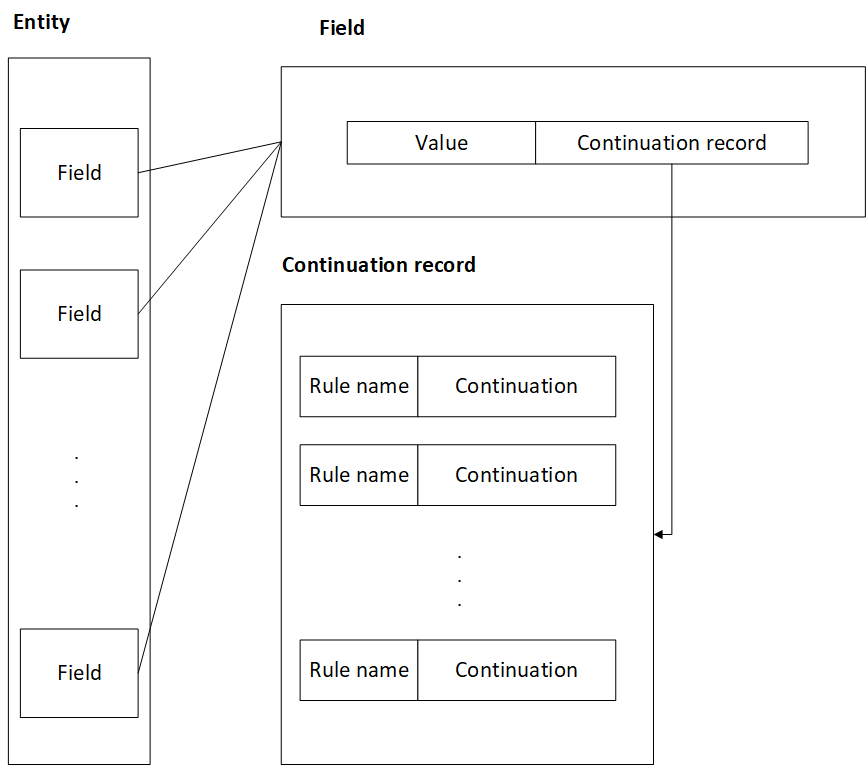
\includegraphics[width=\textwidth]{Figures/chapter_networking/interruptible_rules}
  \caption{Schematic representation of the implementation of the interruptible rules}
  \label{fig:ch_networking_interruptible_rules}
\end{figure}

A field of the entity record must be adapted now to contain not only the field value, but a record instance used to store the continuations of the Casanova rules affecting that field. Since a record requires a name for each field, we can expand the coroutine functor to take a string representing an identifier for each rule and the continuation record itself:

\begin{lstlisting}
Functor "Coroutine" => string => Record => Record => string => stmt : FieldUpdater


---------------------------
Coroutine ruleId continuation r name => FieldUpdater r name {
  ...
}
\end{lstlisting}

\noindent
Now the first string in the declaration of the functor represents the rule identifier, while the other arguments have the same semantics (record and field of the record the rule can modify). When a Casanova statement requires to store the continuation it can use \texttt{ruleId} to build the setter for the record field of the continuation record. It then calls the function \texttt{set} from the setter module instance to save the continuation of each rule. In this way every rule acting on the record is able to store separately its continuation in the continuation record. As an example, we provide below the evaluation rule for the \texttt{wait} statement that updates the continuation in this implementation:

\begin{lstlisting}
t > 0.0
GetField r name => getter
getter.get entity -> (v,cont)
SetField cont ruleId => continuationSetter
continuationSetter.set (wait(t - dt);k) -> cont'
---------------------------------------------
eval_s entity (wait t;k) dt => (v,cont')
\end{lstlisting}

\noindent
Another aspect that has not been considered yet is how to define variables local to the rule (local bindings). Since the set of local bindings is known at compile time, we can modify the continuation record to store not only the continuation itself, but also the state of the local bindings as record of bindings. In this way an element of the continuation record, that we can now call rule state, stores not only the statements of the rule left to evaluate but also the state of the local bindings. When we need to read the value of a binding or update it, we can again use a getter or setter by accessing the rule state and getting or setting the appropriate field for the binding from the binding record. A schematic representation of this implementation can be seen in Figure \ref{fig:ch_networking_interruptible_rules_with_state}.

\begin{figure}
  \centering
  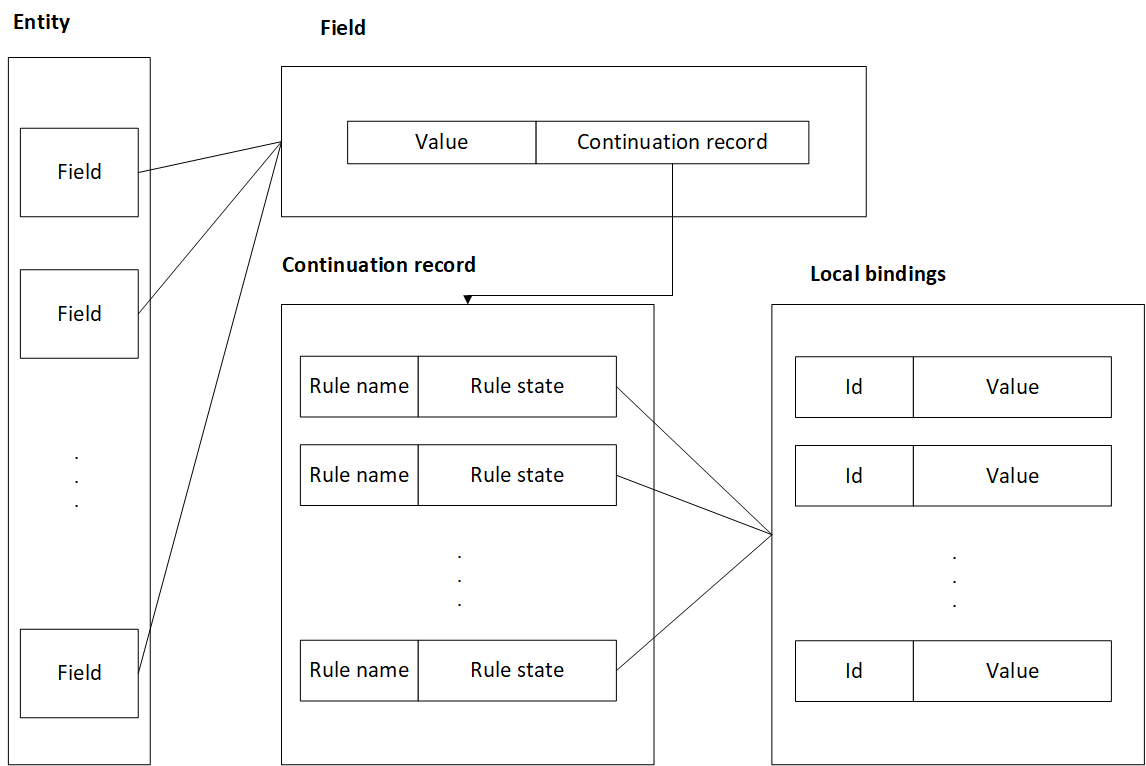
\includegraphics[width=\textwidth]{Figures/chapter_networking/interruptible_rules_with_state}
  \caption{Schematic representation of the implementation of interruptible rules with local bindings}
  \label{fig:ch_networking_interruptible_rules_with_state}
\end{figure}

As final remark, we point out that the use of records to store the rule continuations and local bindings show how the record optimization introduced in Chapter \ref{ch:functors} can also be adapted to implement a generic symbol table to store various information regarding the language elements that are needed during the execution of the generated code, thus making this approach extremely flexible for different situations.

\section{Evaluation}
\label{subsec:ch_functor_languages_evaluation}
In the previous sections we showed how to use functors to implement the entity update traversal of the domain-specific language for game development Casanova. Based on the preliminary analysis performed in Chapter \ref{ch:functors}, we claimed that using functors would improve the performance of the implementation of Casanova in Metacasanova given in Chapter \ref{ch:languages} by, at the same time, inlining the access to the entity fields and pre-building the traversal for the Casanova program at compile time, instead of dynamically accessing the fields from a dictionary and inspecting their type to perform the update traversal at every update. In this section we show the experimental results that show the performance of this implementation in comparison to the first dynamic implementation presented in Chapter \ref{ch:languages}.

\subsection{Experimental Setup}
For this evaluation we have implemented the physical body simulation that was presented in the previous sections. The simulation has been run for 10000 frames, which roughly correspond to 3 minutes assuming an average update rate of 60 frames/second, with a number of physical bodies ranging from 100 to 1000. Each physical body is randomly generated, that is, its initial position, velocity, and acceleration is randomly generated. We measured the time at the beginning and at the end of the execution of the whole simulation and we averaged the total time by the number of frames the simulation has been running for. We then compared the result with what obtained for the implementation shown in Chapter \ref{ch:languages}.

\subsection{Results}
In Table \ref{tab:ch_networking_evaluation} we can see that the update time is in the order of milliseconds or one tenth of milliseconds where the dynamic implementation was in the order of one hundredth of seconds with 1000 entities. This corresponds roughly to a frame rate of 939 frames/second for the functor implementation versus 28 frames/second. The performance gain ranges from a maximum of 55.397 to a minimum of 33.117 times with an avarage gain of 42.508 times. This comes with no surprise, since in Section \ref{sec:ch_functors_evaluation} we tested the gain of accessing record fields with the functor implementation compared to the dynamic tables, and we had an average gain of roughly 11 times. The gap with the dynamic implementation here is even greater because, to the cost of accessing dynamic tables at runtime to retrieve the values of the entity fields, we have to add the performance loss of performing the update traversal and the rule execution dynamically. Figure \ref{fig:ch_networking_chart} shows a chart where the horizontal axis represents the number of entities in the simulation, while the horizontal axis represents the average frame update time with that number of entities in seconds.

To conclude, we want to point out that this evaluation is a worst-case scenario, since the implementation shown in this Chapter makes use exclusively of Metacasanova meta-data structures to represent the values of the entity fields while the simulation shown in Chapter \ref{ch:languages} uses \texttt{Vector2} from the Monogame library. This means that this simulation has an additional overhead due to accessing the components of a tuple via pattern matching, and due to the use of value types versus reference types. The performance shown here could be improved by using \texttt{Vector2} from an external library instead of \texttt{Tuple[float, float]} to store the position, velocity, and acceleration of a physical body.
\begin{table}
  \centering
  \resizebox{\textwidth}{!}{
  \begin{tabular}{|c|c|c|c|}
  \hline
  \textbf{Entity number} &\textbf{Update time (functors)} &	\textbf{Update time (dynamic)} &	\textbf{Performance Gain} \\
  \hline
  100 &	0.000063 & 0.00349 & 55.397\\
  \hline
  250 &	0.000173 & 0.00911 & 52.659\\
  \hline
  500 &	0.000428 & 0.01716 & 40.093\\
  \hline
  750 &	0.000777 & 0.02597 & 33.423\\
  \hline
  1000 & 0.001065 &	0.03527 & 33.117\\
  \hline
  \multicolumn{2}{c|}{} & \textbf{Average gain} & 42.938 \\ \cline{3-4}	
  \end{tabular}}
 	\caption{Update time for one frame of the functor implementation of Casanova and the dynamic implementation shown in Chapter \ref{ch:languages}. The time is measured in seconds}
  \label{tab:ch_networking_evaluation}
\end{table}

\begin{figure}[!h]
  \centering
  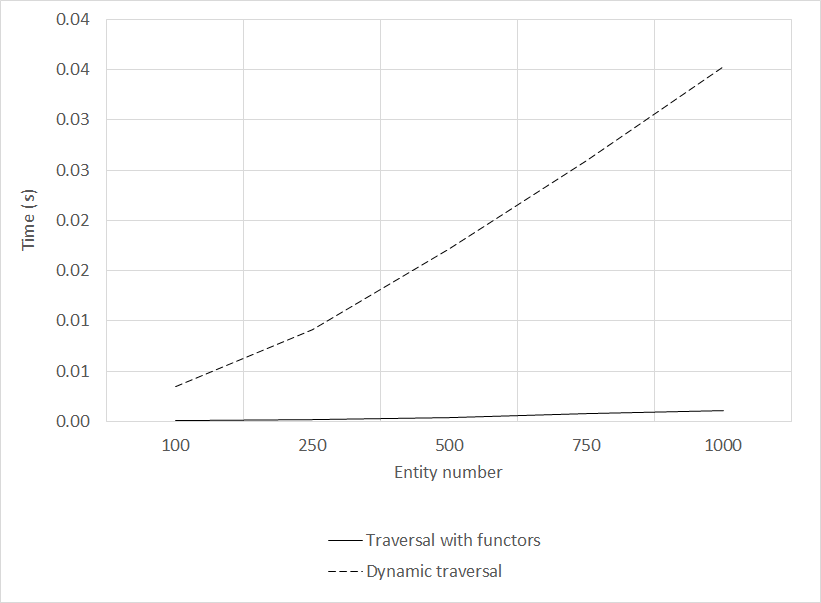
\includegraphics[width=\textwidth]{Figures/chapter_networking/chart}
  \caption{Execution time of Casanova implemented with functors vs the dynamic implementation}
  \label{fig:ch_networking_chart}
\end{figure}

\section{Summary}
In this chapter we proposed a new implementation of the semantics of Casanova based on the language extension with functors and modules presented in Chapter \ref{ch:functors}. We showed that functors and modules are expressive enough to implement the logic of the entity update in Casanova and at the same time to allow rule interruption. At the same time, functors grant static typing and the inlining of ad-hoc update functions depending on the structure of the entity we need to update. This improvement increases the performance of this new implementation of Casanova on average by roughly 42 times. This improvement makes the implementation of Casanova suitable for game development, as the generated code is now able to process at more than 900 frames/second versus the 28 of the previous implementation.


\chapter{Networking in Casanova}
\label{ch:networking}
\epigraph{The Internet is not just one thing, it's a collection of things - of numerous communications networks that all speak the same digital language.}{Jim Clark}
In this section we introduce the basic concepts of the implementation of multiplayer game development for Casanova 2. This implementation aims to relieve the programmer of the complexity of hard-coding the network implementation for an online game, while preserving encapsulation in code. We show that code analysis is required to generate the appropriate network primitives to send and receive data. Finally, we present a simple multiplayer game to show a concrete example.

\section{Introduction}
Adding multi-player support to games is a highly desirable feature. By letting players interact with each other, new forms of gameplay, cooperation, and competition emerge without requiring any additional design of game mechanics \cite{granberg2014david}. This allows a game to remain fresh and playable, even after the single player content has been exhausted. For example, consider any modern AAA (AAA refers to games with the highest development budgets\cite{wolf2008video}) game such as \textit{Halo 4}. After months since its initial release, most players have exhausted the single player, narrative-driven campaign. Nevertheless the game remains heavily in use thanks to multiplayer modes, which in effect extended the life of the game significantly. This phenomenon is even more evident in games such as \textit{World of Warcraft} or \textit{EVE}, where multiplayer is the only modality of play and there is no single-player experience.

\paragraph{Challenges}
Multi-player support in games is a very expensive piece of software to build. Multiplayer games are under strong pressure to have very good \textit{performance} \cite{claypool2006latency}. Performance is both expressed in terms of CPU time and in bandwidth used. Also, games need to be very \textit{robust} with respect to transmission delays, packets lost, or even clients disconnected. To make matters worse, players often behave erratically. It is widespread practice among players to leave a competitive game as soon as their defeat is apparent (a phenomenon so common to even have its own name: ``rage quitting'' \cite{rage_quitting}), or to try to abuse the game and its technical flaws to gain advantages or to disrupt the experience of others.

Networking code reuse is quite low across titles and projects. This comes from the fact that the requirements of every game vary significantly: from turn-based games that only need to synchronize the game world every few seconds, and where latency is not a big issue, to first-person-shooter games where prediction mechanisms are needed to ensure the smooth movement of synchronized entities, to real-time strategy games where thousands of units on the screen all need to be synchronized across game instances \cite{smed2002aspects}. In short, previous effort is substantially inaccessible for new titles. 

Encapsulation suffers from this ad-hoc nature of the implementation of the networking layer in multiplayer games. Indeed managing the information about game updates over a network requires each game entity to interface the game logic code with network connection and socket objects, data transmission method calls such as send and receive, and support data structures to manage traffic and track the status of common protocols. This happens because each game entity must provide the following functionality in order to work in a multiplayer game:

\begin{itemize}
	\item Update the logic in the fashion of a singleplayer counterpart.
	\item Choose what data is necessary to send over the network and create the message containing this information.
	\item Choose what data can be lost and what data must always be received by the other clients.
	\item Periodically check if incoming messages contain information that needs to be read and to perform specific updates.
\end{itemize}

Combining these requirements together within the same entity breaks encapsulation because now the logic of the entity and lots of spurious details only relevant to the networking implementation are mixed together, resulting in a highly noisy program. Maintenance then becomes very hard, as every change in the game logic must also be reflected in the networking implementation.

\paragraph{Existing approaches}
Networking in games is usually built with either very low-level or very high-level mechanisms. Very low-level mechanisms are based on manually sending streams of bytes and serializing only the essential bits of the game world, usually incrementally, on unreliable channels (UDP). This coding process is highly expensive because building by hand such a low-level protocol is difficult to get right, and debugging subtle protocol mismatches, transmission errors, etc. will take lots of development resources. Low-level mechanisms must also be very robust, making the task even harder.

High-level protocols such as RDP, reflection-based serialization, frameworks (such as Pastry, netty.io), etc. can also be used. These methods greatly simplify networking code, but are rarely used in complex games and scenarios. The requirements of performance mean that many high-level protocols or mechanisms are insufficient, either because they are too slow computationally (especially when they rely on reflection or events) or because they transmit too much data across the network.

\section{Motivation}

To avoid the problems of both existing approaches, we propose a middle ground. We observe that networking fundamental abstractions upon which the actual code and protocols are built do not vary substantially between games, even though the code that needs to be written to implement them does. The similarity comes from the fact that the ways to serialize, synchronize, and predict the behaviour of entities are relatively standard and described according to a limited series of general ideas. The difference, on the other hand, comes from the fact that low-level protocols need to be adapted to the specific structure of the game world and the data structures that make it up. Until now, common primitives have not been syntactically and semantically captured inside existing domain-specific languages for game development \cite{bhatti2009domain}. Using the right level of abstraction, these general patterns of networking can be captured, while leaving full customization power in the hand of the developer (to apply such primitives to any kind of game).

\section{Related work}
In the following we discuss some existing networking tools used in game development and we highlight some issues that arise from their use.

\paragraph{The Real time framework (RTF)} RTF \cite{glinka2007rtf} is a middleware built for C++ to relieve the programmer from dealing with data compression. It is more flexible than solutions based on game engines or hand-made implementations, since it automates the process of data transmission. Moreover, it supports distributed server management. Unfortunately, this solution has several flaws:
\begin{itemize}
	\item All entities must inherit from the class \texttt{Local} and the semantics of the position is pre-determined, often clashing with rendering or physics.
	\item Platform independence requires that the programmer uses RTF primitive	types.
	\item Data transmission automation requires that all game entities inherit the class \texttt{Serializable}.
	\item Being a middleware, RTF is not aware of what games are going to use it for (every game comes with different data structures). Thus, the developer is tasked to include in his code also logic to update the RTF layer, in order to keep the game updated over the network.
\end{itemize}


\paragraph{Network scripting language (NSL)} NSL \cite{russell2008tackling} provides a language extension based on a send-receive mechanism. Moreover it provides a built-in client side prediction (a feature missing in existing highly concurrent and distributed languages such as Stackless Python \cite{kalogirou2005multithreaded} and Erlang \cite{armstrong1993concurrent}), which is periodically corrected by the server. 

\paragraph{Unreal Engine/Unity Engine} Unreal Engine \cite{games2006unreal} and Unity Engine \cite{engine9unity} are commercial game engines supporting networking.  Both Unity and Unreal Engine use a client-server approach. In Unreal Engine, the server contains the ``true'' game state, and the clients contain a ``dirty'' copy, which is validated periodically. It is possible to define entities (actors in Unreal Engine jargon) that are replicated on the clients. Whenever a replicated actor changes on the server, this change is also reflected on the clients. Additional customization can be achieved through Remote procedure calls (RPCs) of three kinds.
\begin{itemize}
	\item The function is called on the server and executed on the client. This is used for game elements that do not affect gameplay, such as creating a particle effect when a weapon is fired.
	\item The function is called on the client and executed on the server. This is useful for events that affect the other clients and should be validated by the server.
	\item The function is executed in multi-cast, meaning that the server calls the function and that it is executed on both the server and all the clients.
\end{itemize}

The Unity Engine uses a similar approach based on networking components, synchronized at every frame, and RPC's to define custom synchronization events.

Unfortunately, customization comes at the cost of the level of detail that developers must face. Using RPC's require a deep knowledge of the engine and writing lots of code, as discussed in Section \ref{Common issues}.

In this section we introduce a small example that addresses the requirements of designing a multiplayer game. We then present an architecture that aims to fulfil these requirements.

\section{The master/slave network architecture}

We chose to implement the networking layer in Casanova 2 by using a peer-to-peer architecture for the following reasons:

\begin{itemize}
	\item Server-client architectures are more reliable but suitable only for specific genres of games (mostly Shooter games), while other genres, such as Real-time strategy games or Online Role Playing Games, use P2P architectures.
	\item We do not have to write a separate logic for an authoritative game server, which has to validate the actions of clients.
\end{itemize}

Casanova will provide a generic tracking server, which is run separately from the main program. The tracking server is a thin service that connects players participating in a single game, and helps with forwarding the network traffic through NATs (Network Address Translation).

Each client maintains a local copy of the \texttt{world} entity and has direct control over a single portion of it. Instances belonging to such as portion are seen as \textit{master} by this player, who is always allowed to directly change the state of the master instances without having to validate this state change by synchronizing with other players through the network.

Each client also maintains a portion of the world that is not directly under his control. Instances belonging to such as portion are seen as \textit{slave} by this player, who is only allowed to \textit{predict} the local state of the instances and, whenever he receives an update from their masters, must correct this prediction according to the data contained in the received messages. The slave part of the world is thus maintained passively by the client: the only active part is predicting the evolution of the entity state and correcting it whenever he receives an update by its master.

For this purpose, we extend the syntax of Casanova rules by allowing them to be marked with the modifiers \texttt{master} and \texttt{slave}. These rules are executed respectively on master and slave entities. Note that it is still possible not to mark a rule with these modifiers, which means that the rule is always executed independently of the fact that the entity is either master or slave on that particular client. We also allow to mark a rule as \texttt{connecting} and \texttt{connected}. These rules are triggered only once respectively when a new client connects and when the clients detect a new connection.

Casanova also provides primitives to send (reliably or unreliably) and receive data. A schematic representation of this architecture can be seen in Figure \ref{fig:masterslave}.

\begin{figure}[h!]
	\centering
	\caption{Representation of the game world in a networking scenario}
	\label{fig:network_world}
	\begin{subfigure}[t]{0.3\linewidth}
		\centering
		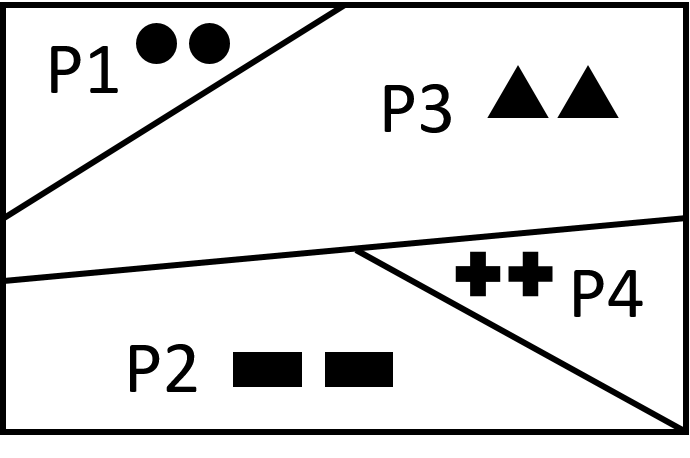
\includegraphics[width=1\linewidth]{Figures/networking2}
		\caption{Unknown correct game state when P3 joins the game.\\}
		\label{subfig:networking_ideal}
	\end{subfigure}
	\begin{subfigure}[t]{0.3\linewidth}
		\centering
		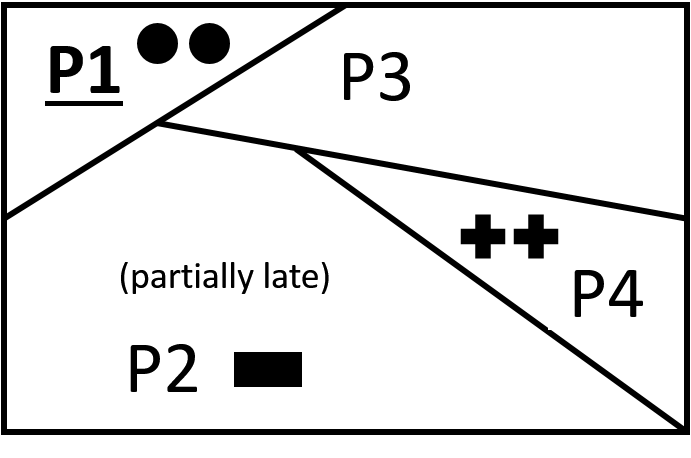
\includegraphics[width=1\linewidth]{Figures/networking1}
		\caption{Networking game state seen from the point of view of P1. P2 is partially synchronized, P4 is fully synchronized, and P3 is a new client that is late and is still sending its data}
		\label{subfig:networking_relative}
	\end{subfigure}
	
	
\end{figure}

\begin{figure}
	\centering
	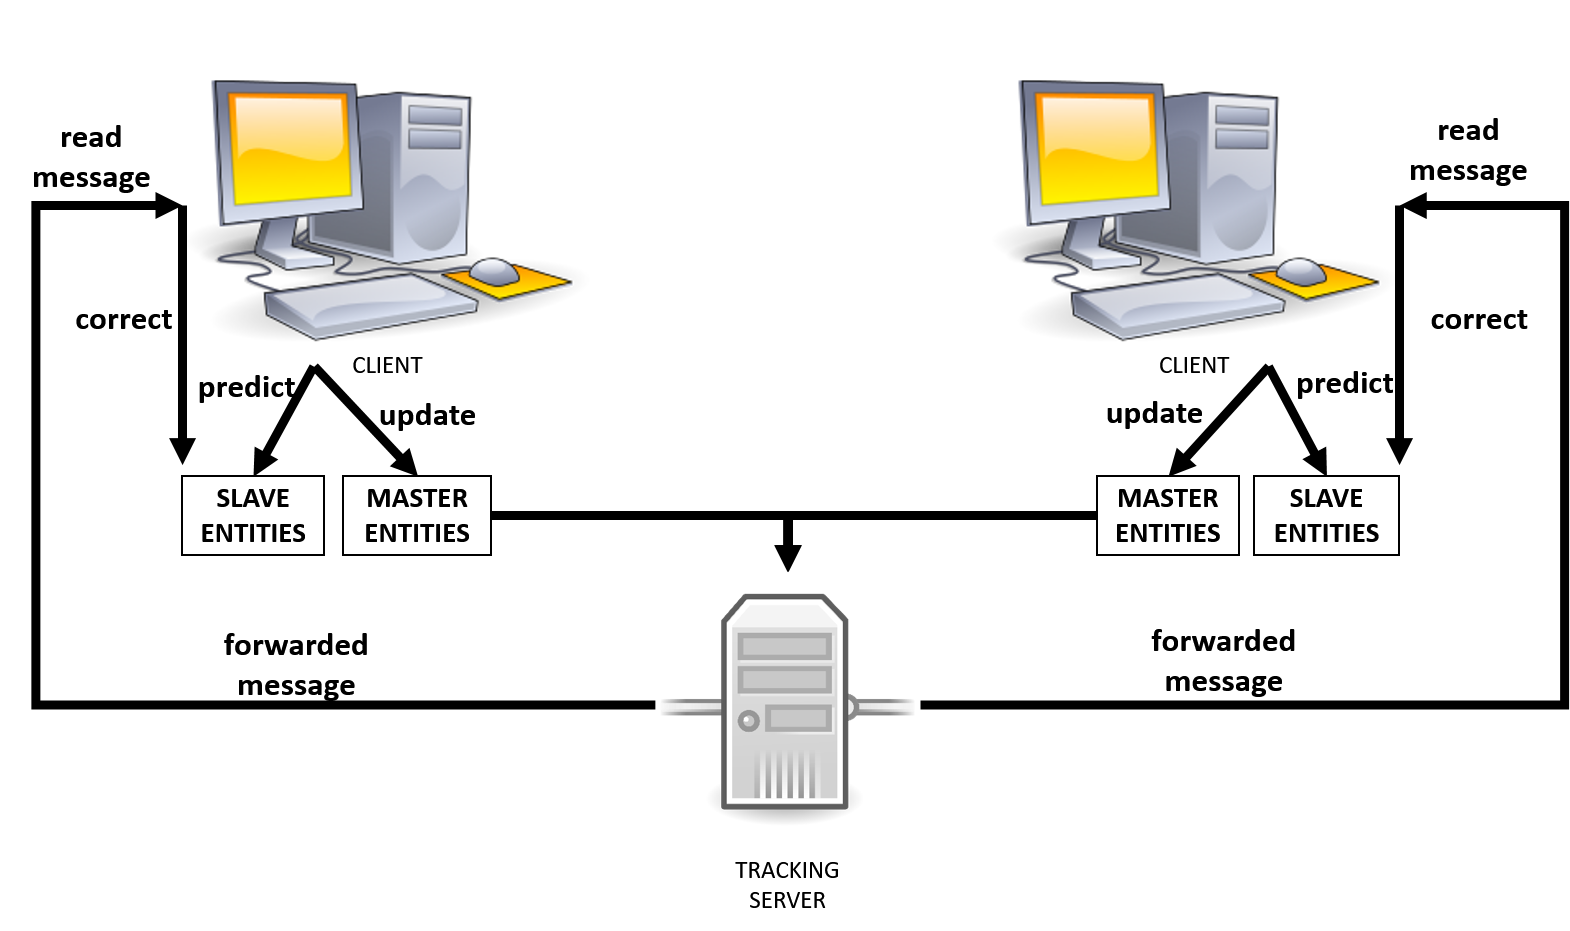
\includegraphics[width = \textwidth]{Figures/masterslave}
	\caption{master/slave architecture}
	\label{fig:masterslave}
\end{figure}

Note the aim of this architecture is to provide language-level primitives to describe the networking logic. This means that the compiler will be able to generate code compatible with the low-level network libraries that provide transmission functions over the network channel without having to change Casanova code in the program. In our implementation, we chose the .NET library \texttt{Lidgren}, which is widely used also in commercial game engines such as Unity3D and MonoGame, but nothing prevents the compiler to be expanded in order to target other similar libraries for other languages, such as jgroups \cite{ban2002jgroups}.

\section{Case study}
Let us consider a simple shooter game where each player controls a space ship. Players can move forward, backward, and rotate the ship to change direction. Moreover, they can use the ship lasers to shoot other players. If a laser hits an enemy ship, we increase the player's score. Designing such a game requires to address the following issues, depicted by the schematic representation in Figure \ref{fig:network_world}:

\begin{enumerate}
	\item Each player must maintain a local version of the game state (world). In order to avoid to flood the network with messages, all the copies are not fully synchronized at each frame, thus they are slightly different and each client knows the latest version of only part of the copy.
	\item A player \texttt{connecting} to an existing game must be able to receive the latest update of the game state and send the new ship he will control to existing players in the game.
	\item A player already \texttt{connected} to the game must detect a new connection and send his master portion of the game state.
	\item Each player must be able to control only one ship at a time. This means that the part of the game logic that processes the input and modifies the spatial data of the ship (position and rotation) should only be executed on the ship controlled by the player and not on the local copies of other players' ships. This means that each player sees as \texttt{master} only one ship instance.
	\item Each player must send the updated state of the ship he controls to the other players after executing the local update. To achieve better performance over the network, the data is not sent at every update, but with a lower frequency.
	\item Each player must receive the updated state of \texttt{slave} ships controlled by other players. In this phase, we must take into account that, as explained above, not every update is sent, so the player should ``predict'' what will happen during the game frames in which he does not receive an update.
\end{enumerate}

\section{Implementation}
Each of the scenarios described above requires specific language extensions. These extensions identify connection, ownership (master/slave), and various send and receive primitives. In this section, we introduce each primitive by using a multiplayer game example \footnote{The game source code and executable can be found at \url{https://github.com/vs-team/casanova-mk2/wiki/Networking-extension}}. We now give an implementation of the shooter game presented above, using the extended version of Casanova 2 with network primitives. 

The \texttt{world} contains a list of ships controlled by each player.
\begin{lstlisting}
world Shooter = {
Ships  : [Ship]
...
}
\end{lstlisting}

Each \texttt{Ship} contains a position, a rotation, a collection of shot projectiles, and the score.
\begin{lstlisting}
entity Ship = {
Position   : Vector2
Rotation   : float32
Projectiles : [Projectile]
Score		  : int
...
}

\end{lstlisting}

Each \texttt{Projectile} contains its position and velocity.

\begin{lstlisting}
entity Projectile = {
Position : Vector2
Velocity : Vector2
...
}
\end{lstlisting}

\subsubsection{Connection}
When a player connects, we must consider two different situations: (\textit{i}) a player is already in the game and must send the current game state to the connecting players, and (\textit{ii}) the player who is connecting needs to send the ship he will instantiate and control (its initial state). Both the players in the game and the connecting one must receive the game states that are sent. For this purpose we introduce two additional modifiers, \texttt{connecting} and \texttt{connected}, that can be added to rule declarations to mark their role in the multiplayer logic.

\paragraph{Connecting} A rule marked with \texttt{connecting} is executed once when a player joins the game for the first time. In our example, the player should send his initial state (the created ship) to the other players. We use the primitive \texttt{send\_reliable} because we must be sure that eventually all players will be notified of the ship creation.
\begin{lstlisting}
world Shooter = {
...
rule connecting Ships =
yield send_reliable Ships
}
\end{lstlisting}

\paragraph{Connected} A rule marked with \texttt{connected} is run whenever a new player joins the game by all existing players. When this occurs, each player sends its ship. The system will take care to send only the ship controlled locally by the player itself for each player. The rule will use the \texttt{send\_reliable} primitive for the same reason explained in the previous point.

\begin{lstlisting}
world Shooter = {
...
rule connected Ships =
yield send_reliable Ships
}
\end{lstlisting}

Note that even if the code is the same, the semantics of the two rules are different. The first one is executed by the player joining the game, who locally instantiates its \texttt{Ship} and must send its list of \texttt{Ships} (containing only the local instance) to the other players. The second one is executed by all existing players who must share with the joining player the list of existing ships.


\subsubsection{Master updates}
As explained above, each client manages a series of local game objects (called \textit{master objects}) that are under its direct control. The other clients read passively any update done on those instances and update their remote copy  (\textit{slave objects}) accordingly. We mark rules affecting the behaviour of master objects as \texttt{master}. In our example, the following situations are run as master: (\textit{i}) synchronizing the ships among players, (\textit{ii}) updating the ship and projectiles spatial data, and (\textit{iii}) creating and destroying projectiles.

\begin{enumerate}
	\item Each player is tasked to maintain the list of Ships in the world. This requires to receive the updated list from other players and to store the new value in a master rule. Indeed the world is a special case of an entity that is shared among players, and not directly owned by somebody. Each ship contained in that list and received from other players will be treated appropriately as slaves, while the only one owned by the current player will be under his direct control. In this rule we use \texttt{let!}, which is an operator that waits until the argument expression returns a result and then binds it to the variable. The symbol \texttt{@} stands for list concatenation. The rule uses \texttt{receive\_many}, which receives and collects the list of sent ships by the other players.
	
	\begin{lstlisting}
	world Shooter = {
	...
	rule master Ships =
	let! ships = receive_many()
	yield Ships @ ships
	}
	\end{lstlisting}
	
	\item The master version of the ship update reads the input of the player and moves (or rotates) the ship if the appropriate key is pressed. Note that this part must be executed only on a master object, because we want to allow each player to control only the ship he owns and instantiates at the beginning of the game. Below we show just the rule to move forward; the other movement and rotation rules are analogous. We use an \textit{unreliable send} because it is acceptable to lose an update of the position during a certain frame: shortly after, there will be a new update.
	
	\begin{lstlisting}
	entity Ship = {
	...
	rule master Position =
	wait world.Input.IsKeyDown(Keys.W)
	let vp = new Vector2(Math.Cos(Rotation), 
	Math.Sin(Rotation)) * 300.0f
	let p = Position + vp * dt
	yield send p
	}
	\end{lstlisting}
	
	We do the same for projectiles, except the projectile position is continuously updated and synchronized over the network without having to wait that a key is pressed.
	
	\item Creating a new projectile happens when the player shoots. A ship keeps track of the projectiles it has shot so far, and adds a new one to the list of the existing projectiles. The updated list is sent to all players with the new instance of the projectile (which is added as a new head of the list with the operator \texttt{::}). Here it is better to precise the semantics of the \texttt{yield} in conjunction with the use of networking primitives. A \texttt{yield} requires that the written value is type-compatible with the domain of the rule. Thus, when used with a \texttt{send} primitive, we must pass as argument a list. The system will ensure, for performance reasons, that the generated code only sends the new items added to the list. This semantics is defined as such for two main reasons: (\textit{i}) when sending the new projectiles we must also update the list in local (and given the immutability of Casanova we must replace the existing one), and (\textit{ii}) because in this way the programmer can focus on the logic of the game as if it were a single-player game without worrying of network-specific details. Note that the last \texttt{wait} forces the player to release the key before shooting again (semi-automatic fire). Removing that check would spawn multiple projectiles consecutively, which is not a wanted behaviour.
	
	\begin{lstlisting}
	entity Ship = {
	...
	rule master Projectiles =
	wait world.Input.IsKeyDown(Keys.Space)
	let vp = new Vector2(Math.Cos(Rotation), 
	Math.Sin(Rotation)) * 500.0f
	let projs = new Projectile(Position, vp) :: Projectiles
	yield send_reliable projs
	wait not world.Input.IsKeyDown(Keys.Space)
	}
	\end{lstlisting}
	
	Filtering the colliding projectiles and updating the score is run as a master rule. The rule computes the set difference between the ship projectiles and the colliding projectiles and updates the list of projectiles, sending them through the network as well. Even in this case, the network layer sends only the information about the projectiles to remove. Note that the score is managed by each player locally, as it does not require to be synchronized (we do not print the other players' scores. Doing so would indeed require to also send the score).
	
	\begin{lstlisting}
	entity Ship = {
	...
	rule master Projectiles, Score =
	let collidingProjs =
	[for p in Projectiles do
	let ships =
	[for s in Ships do
	where 
	s <> this and 
	Vector2.Distance(p.Position,s.Position) < 100.0f
	select s]
	where ships.Count > 0
	select p]
	let newProjectiles = Projectiles - collidingProjs
	yield send_reliable newProjectiles, 
	Score + collidingProjs.Count 
	}
	\end{lstlisting}
\end{enumerate}

\subsubsection{Managing remote instances}
The game objects that were not instantiated by a client, but received from another client, are \textit{slave objects} and must be synchronized differently than master objects. For this purpose, a rule can be marked as \texttt{slave}. In our example, we use slave rules in the following situations: (\textit{i}) synchronizing other players' ships and projectiles spatial data, and (\textit{ii}) projectiles instantiated by other players.

\begin{enumerate}
	\item Every remote projectile and ship is synchronized locally by a rule, which tries to \texttt{receive} a message containing updated spatial data. Below we provide the code to update the position of the ship; the synchronization of other spatial data is analogous.
	
	\begin{lstlisting}
	entity Ship = {
	...
	rule slave Position = yield receive()
	}
	\end{lstlisting}
	
	\item When a projectile is instantiated remotely, we have to receive it and add it to the list of projectiles. We use \texttt{receive\_many} because the new projectiles are added to a list. This case also supports the situation where a ship could shoot multiple projectiles at the same time.
	
	\begin{lstlisting}
	entity Ship = {
	...
	rule slave Projectiles =
	let! projs = receive_many()
	yield projs @ Projectiles
	}
	\end{lstlisting}
\end{enumerate}

In this scenario is important to discuss the atomicity of these transmissions: in the context of network games, reliability is often sacrificed for better network performance, so most of the data transmissions are unreliable (like in the case of the ship position). This means that we have no guarantee that the message will be received. Several issues can arise from this situation: for example, if a player fails to receive the position of the ship, then it might miss a collision with a projectile. This is a well-known issue in several shooter games and out-of-sync errors might happen during a multiplayer game. However, ensuring that all the data transmissions are reliable might affect network performance to the point that the game would become unplayable because of the network overload. 

Casanova 2 allows the programmer to decide whether the transmission should be reliable or not and experiment with the effect of a reliable transmission versus an unreliable one that does not overload the network. For example, the updated list of projectiles, after a collision, is always sent in a reliable way. This is acceptable because collisions are not so frequent. This is not true for the ship position, since movements are very frequent and mostly happen at every frame, thus it is something that should not be sent reliably at every frame.

Furthermore, we want to focus the attention on the implicit relationship between this networking architecture and the encapsulation: as shown for instance in the examples where the ship shoots a projectile, we ensure encapsulation by keeping a semantics that filters completely the details about networking. The programmer only worries about the logic of adding a new projectile, while the details of the network transmission are hidden. A hand-made implementation is usually prone to break this separation of concerns because the transmission logic is tightly coupled within the game logic itself.

\section{Entity update with functors in Metacasanova}
\label{sec:ch_networing_entity_update_functors}
In Section \ref{subsec:ch_mcnv_languages_casanova_semantics} we showed an implementation in Metacasanova of Casanova, a domain-specific language for game development, while in Section \ref{subsec:code_generation_discussion} we discussed about the reason of the poor performance of that implementation. In Chapter \ref{ch:functors} we extended Metacasanova with functors and modules to allow to embed the type system of an embedded  language \footnote{See the introduction of Chapter \ref{ch:functors} for a definition of this term} in the meta-compiler to overcome the problem of dynamic lookups at runtime. We then showed an implementation of records with modules and functors that significantly improved the performance of memory accesses, as shown in Section \ref{sec:ch_functors_evaluation}. In what follows we discuss another problem related to the implementation of Casanova and we provide an alternative implementation using functors that builds upon the existing implementation of records described in Section \ref{sec:ch_functors_record_implementation}.

\subsection{Casanova entity update}
\label{subsec:ch_networking_casanova_update}
In Section \ref{subsec:ch_mcnv_languages_casanova_semantics} we described the memory representation of a Casanova entity in Metacasanova and how the rules of an entity are updated. What was skipped for brevity was to describe how the system behind Casanova updates the entities of a Casanova program. As briefly described in Section \ref{sec:ch_mcnv_languages_casanova_language}, the structure of a program in Casanova is a tree, whose root is a special entity called \textit{World}. The world entity can contain fields that are instances of other entities as well, thus creating an additional level in the program tree. This is, of course, allowed also for regular entities, thus the height of the tree is arbitrary. Each entity might contain a set of rules that describe its dynamic behaviour with respect to time, thus they are updated by considering the time difference between the current and the previous update (\textit{frames}). Updating a rule is enforced by traversing the entity tree, thus when the field of an entity is an entity itself, the system will first update the entity instance contained in the field and then update the current entity. Casanova also natively supports lists and tuples as valid data types, and this requires to handle their update as well: a tuple or a list might themselves contain instances of entities that must be updated accordingly. In the case of a list of entities, we must run the update on each element, while in the case of a tuple we must examine each element and check whether it requires an update or not. This process might become very complex, as list and tuples can be combined together in infinite many ways, thus the process recursively calls the proper update depending on the type of the field.

At this purpose, let us consider a simulation consisting of an arbitrary amount of physical bodies, in the fashion of what was used in Section \ref{subsec:ch_functors_casanova_example}. The world entity will contain a list of physical bodies that are updated during the simulation. The Casanova code that described such a simulation is the following:

\begin{lstlisting}
worldEntity World {
	PhysicalBodies : [PhysicalBody]
}

entity PhysicalBody {
	Position				: Tuple<float,float>
	Velocity				: Tuple<float,float>
	Acceleration		: Tuple<float,float>
	
	rule Position = Position + Velocity * dt
	rule Velocity = Velocity + Acceleration * dt
}
\end{lstlisting}

\noindent
In this simulation, the update starts from \texttt{World}. This entity contains only one field, which is a list of physical bodies. Since \texttt{PhysicalBody} is an entity, the update must be run individually for each element of the list. The world contains no rules so after updating its only field we complete its update. At this point the update of each physical body examines each fields. All fields are represented as a point in a 2D space with a tuple containing two floating-point values. The update will examine each value of the tuple and find that they do not require any update (again because the only language abstractions that exhibit dynamic behaviours are entities). The update will then move on to run the rules that will update the content of \texttt{Position} and \texttt{Velocity}. The update process is sketched in Figure \ref{fig:ch_networking_simulation_update} and can thus be seen as a process that consists of the following steps:

\begin{enumerate}[noitemsep]
	\item An \textit{entity update} that traverses all the fields and rules of the entity and calls the appropriate updater.
	\item A \textit{field update} that is able to update (or not) the field depending on its type. The fields that will be updated have type \texttt{List}, \texttt{Tuple}, or \texttt{Entity}.
\end{enumerate}

\begin{figure}
	\centering
	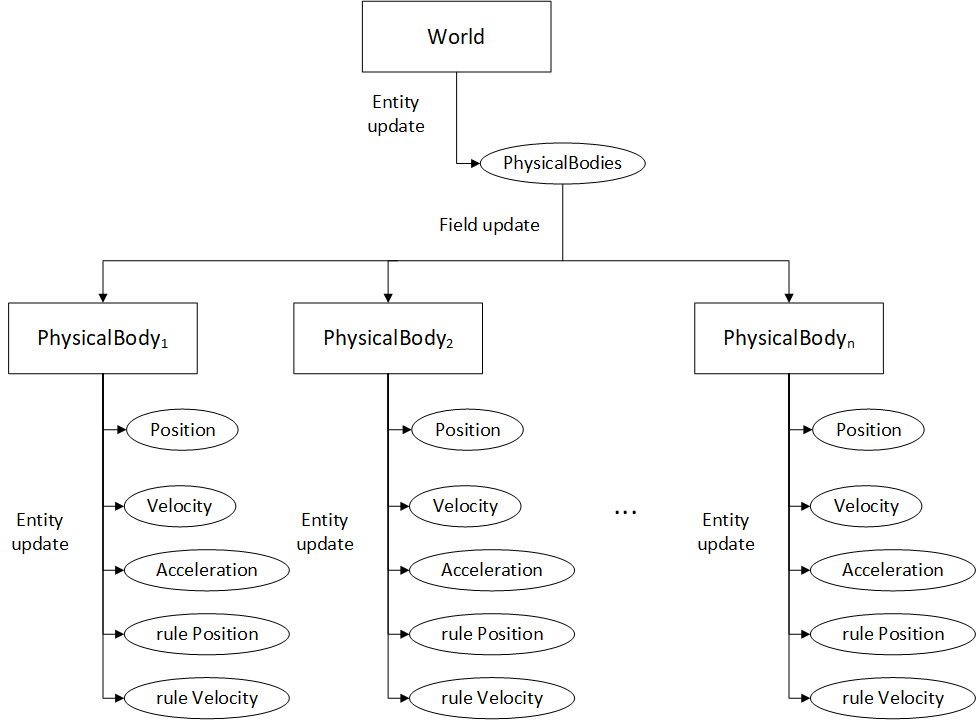
\includegraphics[width=\textwidth]{Figures/chapter_networking/update_traversal}
	\caption{Entity update for the simulation of physical bodies}
	\label{fig:ch_networking_simulation_update}
\end{figure}

\subsection{Update in Metacasanova}
\label{subsec:ch+networking_update_metacasanova}
The update mechanism described in Section \ref{subsec:ch_networking_casanova_update} can of course be integrated in the implementation of Casanova described in Chapter \ref{ch:languages}. In order to do so, we should dynamically look into the dictionary at each update, extract the field and perform an update according to the following cases:

\begin{itemize}[noitemsep]
	\item If the field is a list, then we must examine each element and choose for each one whether it needs to be updated or not. This is done by recursively applying these cases.
	\item If the field is a tuple, then we behave as above.
	\item If the field is an entity, then we must run an update on it.
	\item In all the other cases the field is not updated.
\end{itemize}

\noindent
The cases above are translated into four rules in Metacasanova. The first three will use pattern-matching to decide whether the examined field is a list, a tuple, or an entity. The fourth one is a default rule that simply returns the field as it is. Moreover, each entity should carry with it a list of rules that are updated as well, where all the get and set operations require dynamic lookups in the symbol table of the entity.

Repeating the traversal of the entity tree at each update at runtime is unnecessary since

\begin{itemize}[noitemsep]
	\item The structure of a Casanova entity cannot change at runtime. Its fields and field types will always remain the same.
	\item The fields affected by an entity rule and the rules of an entity do not change during the program execution.
\end{itemize}

\noindent
This means that, by exploiting modules and functors, we are able to specify the structure of the update at compile time and generate directly the function that performs the update at runtime, in the same fashion of what had been done for the record setter and getter. In the following sections we will describe extensively the implementation of the update using modules and functors in Metacasanova that generates at compile time the functions necessary to perform the update of a Casanova program. Note that we will refer to the implementation of records given in Section \ref{sec:ch_functors_record_implementation}.

\subsection{Updater Modules}
\label{subsec:ch_networking_updater_modules}
As explained above, Casanova needs to recursively update fields that are lists, tuples, or entity instances. At this purpose, we define a module that represents an \textit{updatable element} in the Casanova language. The module constructor takes as only argument the type of the element to update. This module contains a function \texttt{update} that is able to update a value of this particular type and uses an additional parameter \texttt{dt} that contains the time difference between the current and the previous update. The function returns the updated value of the element. It also contains an utility functor for the 
 
\begin{lstlisting}
Module "ElementUpdater" => (elementType : *) : ElementUpdater {
	Functor "GetType" : *
	Func "update" -> elementType -> float : elementType
}
\end{lstlisting}

\noindent
The updater for a field is a module constructed by providing the record of the fields, its name as a string, and contains: (\textit{i}) an utility functor that returns the record used in the field updater, and (\textit{ii}) an update function that takes as input an instance of the record, \texttt{dt}, and returns the updated value of the field. We also define an external utility functor \texttt{GetFieldType} that can retrieve the type of a record field given the record it belongs to and its name. The rule for the functor calls the field getter and its \texttt{GetType} functor to retrieve the type of the name. This functor is used by the module constructor to correctly generate the return type of the \texttt{update} function.

\begin{lstlisting}
Functor "GetFieldType" => Record => string : *

GetField r name => getter
getter.GetType => type
---------------------------
GetFieldType r name => type

Module "FieldUpdater" => (r : Record) => (name : string) : FieldUpdater {
  Functor "GetRecord" : Record
  Func "update" -> r.RecordType -> float : (GetFieldType r name)
}
\end{lstlisting}

\noindent
Finally, the updater for a record is a module constructed by providing the record itself and contains: (\textit{i}) an utility functor that returns the type of the record, and (\textit{ii}) a function \texttt{update} that takes the instance of the record, \texttt{dt}, and returns an updated instance of the record.

\begin{lstlisting}
Module "RecordUpdater" => (r : Record) : RecordUpdater {
  Functor "RecordType" : *
  Func "update" -> r.RecordType -> float : r.RecordType
}
\end{lstlisting}

\subsection{Updatable elements}
\label{subsec:ch_networking_updatable_elements}
As explained above, the elements for which the update is needed can be lists, tuples, or entity instances. For this reason we have to create separately three different instances of the module \texttt{ElementUpdater} each one dedicated to updating one of those updatable elements. The first updatable element that we consider is an \textit{entity instance}. The module to update such updatable element uses a \texttt{RecordUpdater} to define how to entity instance should be updated. Indeed updating a field containing an entity instance requires to apply the specific updater for that entity, which in turn returns the updated instance of the entity itself. Thus the declaration for the functor that constructs the proper instance of the module for the entity updater is the following:

\begin{lstlisting}
Functor "UpdateEntity" => RecordUpdater : ElementUpdater
\end{lstlisting}

\noindent
The rule for this functor extract in its premise the type of the record by calling the utility functor \texttt{RecordType} in the record updater passed as parameter to the constructor of the module. The \texttt{update} function uses the record updater to recursively update the entity instance in its premise and then returns the result of this update.

\begin{lstlisting}
recordUpdater.RecordType => recordType
--------------------------
UpdateEntity recordUpdater => ElementUpdater recordType {

	----------------------
	GetType => recordType
 
  recordUpdater.update entity dt -> entity'
  ------------------------------
  update entity dt -> entity'
}
\end{lstlisting}

\noindent
The second updatable element is the list. An updater for a list must take the updater for its elements. Since a list contains elements of the same type, only one updater is required to instantiate its updater module. The functor \texttt{UpdateList} used to generate this module takes one argument which is an \texttt{ElementUpdater}. This is done because the elements of a list could be themselves other lists, entities, or tuples, so we must be able to use their updaters as arguments for this function. The declaration for this functor is thus:

\begin{lstlisting}
Functor "UpdateList" => ElementUpdater : ElementUpdater
\end{lstlisting}

\noindent
The rule for \texttt{UpdateList} extracts in its premise the type of the elements of the list by calling the functor \texttt{GetType} in the element updater provided as input. It then instantiates an \texttt{ElementUpdater} with the type \texttt{List} using as argument for the generic type the type of the element extracted in its premise. The \texttt{update} function for the list is recursive: its base case is the empty list, for which it simply returns an empty list. For a non-empty list the rule for this function uses the element updater in its premise to update the head of the list and then recursively calls the \texttt{update} of the list on the tail to updater the remaining part.

\begin{lstlisting}
updater.GetType => elementType
---------------------------------
UpdateList updater => ElementUpdater List[elementType] {

  -----------------
  GetType => List[elementType]

  --------------------
  update nil dt -> nil

  updater.update x dt -> x'
  update xs dt -> xs'
  -------------------
  update (x :: xs) dt -> (x' :: xs')
}
\end{lstlisting}

\noindent
The updater for tuples is built by defining a functor that takes as input two element updaters, one for the current element of the tuple, and one for the second one. Note that it is possible to recursively provide a tuple updater as a second updater to support the update of tuples containing more than two elements. For example, the updater for \texttt{Tuple[PhysicalBody,Tuple[PhysicalBody,\\PhysicalBody]]} would require to pass an entity updater and recursively a tuple updater. The declaration of this fuctor is thus:

\begin{lstlisting}
Functor "UpdateTuple" => ElementUpdater => ElementUpdater : ElementUpdater
\end{lstlisting}

\noindent
The rule for \texttt{UpdateTuple} uses in its premises \texttt{GetType} from the first updater and the second updater to obtain the types of the first and second element of the tuple. It then instantiates \texttt{ElementUpdater} with the tuple type called with the type of the first and second element as arguments for the generics. The \texttt{update} function runs the \texttt{update} of the first updater on the first element of the tuple and the second updater on the second element.

\begin{lstlisting}
updater.GetType => firstType
nextUpdater.GetType => nextType
---------------------------------------------
UpdateTuple updater nextUpdater => ElementUpdater Tuple[firstType,nextType] {

  -------------------
  GetType => Tuple[firstType,nextType]

  updater.update x dt -> x'
  nextUpdater.update x' dt -> xs'
  ----------------------
  update (x,xs) dt -> (x',xs')
}
\end{lstlisting}

Finally, we need a \texttt{ZeroUpdate} that is required for fields whose values do not change with respect to time, namely all those that do not fall in the three categories above. The functor \texttt{ZeroUpdate} takes as input any type and builds an \texttt{ElementUpdater} with that type. The rule for \texttt{update} simply returns the value of the field as it is.

\begin{lstlisting}
Functor "ZeroUpdate" => * : ElementUpdater

-----------------------
ZeroUpdate type => ElementUpdater type {

  ----------------
  GetType => type

  ----------------
  update v dt -> v
}
\end{lstlisting}

\subsection{Updatable Fields and Records}
The field updater is instantiated by a functor that takes as input an element updater, a record containing the field, and the name of the field to update. Its declaration is the following:

\begin{lstlisting}
Functor "UpdateField" => ElementUpdater => Record => string : FieldUpdater
\end{lstlisting} 

\noindent
The rule for the \texttt{update} function creates in its premises a field getter through the record and the field name passed as input. It then call the function \texttt{get} of the getter with the record instance taken as input to get the value of the field. It then uses the \texttt{update} function from the element updater taken as input from the functor to update the field.

\begin{lstlisting}
----------------------------------------
UpdateField elementUpdater r name => FieldUpdater r name {

  ---------------
  GetRecord => r

  GetField r name => getter
  getter.get rec -> field
  elementUpdater.update field dt -> field' 
  -----------------------------
  update rec dt -> field'
}
\end{lstlisting}

\noindent
The record updater is built by a functor \texttt{Update} that takes as input a field updater, a record updater to update the next part of the record, and returns an instance of the \texttt{RecordUpdater} module. The rule that evaluates the functor extracts the record from the field updater in its premise and passes it to the module constructor for the record updater. The rule for \texttt{update} generates a setter for the field by using the record and the field name. It then calls the field updater passing the record instance and \texttt{dt} as input. This premise will return the updated value for the field. The following premise uses the \texttt{set} function from the previously generated setter to update the record with the new value of the field. After this step it calls the \texttt{update} function of the record updater passed as function argument, which is recursively able to update the remaining part of the record. The result of this update is then returned as final result. Both the functor declaration and the rule for it are provided below

\begin{lstlisting}
Functor "Update" => FieldUpdater => RecordUpdater : RecordUpdater

fieldUpdater.GetRecord => r
---------------------------
Update fieldUpdater nextUpdater => RecordUpdater r {

  r.RecordType => recordType
  ------------------------
  RecordType => recordType

  SetField r name => setter
  fieldUpdater.update rec dt -> v
  setter.set rec v -> rec'
  nextUpdater.update rec' dt -> updatedRecord
  ----------------------------
  update rec dt -> updatedRecord
}
\end{lstlisting}

\noindent
Note that it is possible to provide different field updaters for the same field, as it is possible that, besides the standard Casanova traversal, one wants to define a custom way of updating the field through a Casanova rule.

In order to stop this otherwise infinite recursive process, we must also generate a record updater that simply returns the record as it is. We build such updater through the functor \texttt{NoUpdate}. This functor takes as input a record and instantiates its updater with it. The updater contains a rule for the \texttt{update} function that simply returns the record as it is. The implementation for this updater is provided below:

\begin{lstlisting}
Functor "NoUpdate" => Record : RecordUpdater

---------------------
NoUpdate r => RecordUpdater r {

  r.RecordType => recordType
  ----------------------
  RecordType => recordType
  
  ----------------
  update r dt -> r
}
\end{lstlisting}

\noindent
Finally, rules can be implemented as a field updater that is instantiated by a functor taking as input the record and the field name. The \texttt{update} function will contain the specific code that the rule will perform. In the following section we will provide the implementation of the physical body simulation and show how to use functors to generate the field updater for rules.

\subsection{Physical Body Simulation with Functors}
\label{subsec:ch_networking_simulation}
In this section we present the implementation with functors of the simulation in Casanova presented in Section \ref{subsec:ch_networking_casanova_update}. The simulation consists of a set of bodies that moves according to their physical properties. As previously done in Section \ref{sec:ch_functors_record_implementation}, we create a functor that builds the record module instance for the physical body:

\begin{lstlisting}
Functor "PhysicalBodyType" : Record

RecordField "Acceleration" Tuple[float,float] EmptyRecord => acceleration
RecordField "Velocity" Tuple[float,float] acceleration => velocity
RecordField "Position" Tuple[float,float] velocity => body
---------------------------
PhysicalBodyType => body
\end{lstlisting}

\noindent
At this point, we define the updaters for the physical body fields. Its fields consist of a tuple with two floating point values. Since floating-point values do not require to be updated in Casanova, we create an updater for the floating-point numbers by using the \texttt{ZeroUpdate} functor that instantiates \texttt{ElementUpdater} with an \texttt{update} function that simply returns the input value.

\begin{lstlisting}
Functor "FloatUpdater" : ElementUpdater

ZeroUpdate float => zero
--------------------------
FloatUpdater => zero
\end{lstlisting}

\noindent
\texttt{ZeroUpdate} calls \texttt{ElementUpdater} with \texttt{elementType := float}. The instance of this module will then contain the following functor rule and function declaration\footnote{Note that the evaluation rule for it is always the same for each instance of a module, so we omit it for brevity}.

\begin{lstlisting}
Func "update" -> float -> float : float

-----------------
GetType => float
\end{lstlisting}

\noindent
At this point we can define the element updater for the \texttt{Tuple} that contains the floating point values. This time we use the functor \texttt{UpdateTuple} to instantiate the \texttt{ElementUpdater} module by passing twice \texttt{FloatUpdater} to it. When we do so, we have that (see the definition of the rule for this functor):

\begin{lstlisting}
updater := FloatUpdater
nextUpdater := FloatUpdater
firstType := updater.GetType := float
nextType := nextUpdater.GetType = float
\end{lstlisting}

\noindent
Thus \texttt{ElementUpdater} will be called with \texttt{elementType := Tuple[float,float]}. This module instance will then contain the following functor rule and function declaration:

\begin{lstlisting}
Func "update" -> Tuple[float,float] -> float : Tuple[float,float]

-----------------------------
GetType => Tuple[float,float]
\end{lstlisting}

\noindent
We now build the field updaters for the two Casanova rules of the physical body. In order to do so, we define two functors that build their field updaters:

\begin{lstlisting}
Functor "PositionRule" : FieldUpdater
Functor "VelocityRule" : FieldUpdater
\end{lstlisting}

\noindent
\texttt{PositionRule} will instantiate \texttt{FieldUpdater} in the following evaluation rule:

\begin{lstlisting}
--------------------------------
PositionRule => FieldUpdater PhysicalBodyType "Position" {

  ---------------------
  GetRecord => PhysicalBodyType

  getPos body -> position
  getVel body -> velocity
  << position + velocity * dt >> -> position'
  ---------------------------
  update body dt -> position'
}
\end{lstlisting}

\noindent
Note that \texttt{getPos} and \texttt{getVel} are functions able to retrieve respectively the position and velocity from a physical body, analogously to what was done in Section \ref{sec:ch_functors_record_getter}. The \texttt{update} function uses these two functions in its premises to retrieve the value of the position and velocity and then updates the position according to the differential equation described in Section \ref{subsec:ch_functors_casanova_example}.


\chapter{Discussion and Conclusion}
\label{ch:discussion}
In this work we addressed the problem of teaching and learning how to program and we proposed the use of a didactic model called GrandeOmega. The web implementation of GrandeOmega was tested on a subset of students from Hogeschool Rotterdam with promising results: the use of the didactic model managed, in some cases, to improve the pass rate of the students, while it always improved their overall performance (measured as a percentage of the maximum score). Furthermore, the classes that did not use GrandeOmega performed generally more poorly to the point that, in one of them, no students managed to successfully complete any of the assignments. The tool is also able to predict with a reliability of 77\% if a student will pass the course on the base of the amount of completed assignments. We can thus conclude that using GrandeOmega boosts the general performance of the students, measured as the percentage of correctly given answers, and, in some cases, improves also the pass rate of the course. On the other hand, students who did not use GrandeOmega at all performed, on average, worse and had a lower passing percentage.

\appendix
\chapter{List Operations with Templates}
\label{app:template}
In this appendix we will show in detail some operations on lists built on top of what presented in Section \ref{sec:ch_background_template_metaprogramming} that can be built by using meta-programming in C++ templates. The goal of this appendix is to convince the reader about the level of complexity of using C++ templates to express meta-programming and why it is preferable to use a dedicated meta-compiler.

\section{Element Getter}
\label{sec:app_templates_getter}
Accessing the n-th element of a list defined with templates mimics the behaviour of the its definition in a functional programming languages given below:

\begin{lstlisting}
let rec nth (n : int) (l : List<'a>) : 'a =
  match l,n with
  | x :: xs,0 -> x
  | x :: xs,_ -> nth (n - 1) xs
\end{lstlisting}

\noindent
The recursion base case is when the index we want to access is 0, which means that we want to access the head of the list. In this case we simply return the head by decomposing the list through pattern matching. In the other case we simply make a recursive call by passing the index decreased by 1 and the tail of the list. In template meta-programming, this is translated into a template that performs the same task:

\begin{lstlisting}
template <typename List> struct Nth<LST, 0> 
{
    typedef typename List::Head result;
};
\end{lstlisting}

\noindent
As shown in Section \ref{sec:ch_background_template_metaprogramming}, the arguments of the function are passed as arguments of the template itself. This version of the template is specialized for the integer 0, which corresponds to the base case of the recursion. The general case of the recursion has a dedicated template as follows:

\begin{lstlisting}
template <typename List, int N> struct Nth 
{
    typedef typename List::Tail Tail;
    typedef typename Nth<Tail, N - 1>::result result;
};
\end{lstlisting}

\noindent
The template contains a type definition for the parameter corresponding to the list tail and another type definition corresponding to the recursive call to another \texttt{Nth} template, this time containing only the tail of the list and the counter decreased by 1. To test this we can use the following sample:

\begin{lstlisting}
template <int N> struct Int 
{
  static const int result = N;
};

typedef List<Int<1>, List<Int<2>, List<Int<3>>>> testList;

int main()
{
  cout << Nth<testList, 2>::result::result << endl;
}
\end{lstlisting}

\noindent
Note that we need to access \texttt{result} twice, because the first \texttt{result} is the type of the head of the list generated by template, which is \texttt{Int}. So calling 

\begin{lstlisting}
Nth<testList, 2>::result
\end{lstlisting}

\noindent
returns \texttt{Int}, that is a type. If we want to access the value stored in \texttt{Int} then we must access the constant integer \texttt{result} contained in it. Note that if we try to access an invalid index in the list, the compiler will complain because it will try to generate a template with the tail of a list that does not exist. In this way something that in a normal program becomes a runtime error is here treated as a compilation error.

\section{Element Existence}
\label{sec:app_templates_existance}
The code that tests the existence of an element within a list is recursive as well and mimics the behaviour of its functional counterpart:

\begin{lstlisting}
let exists (element: 'a) (l : List<'a>) : 'a =
  match l with
  | [] -> false
  | x :: xs when element = x -> true
  | x :: xs -> exists element xs
\end{lstlisting}

\noindent
The function returns \texttt{false} as a base case when the list is empty, because it means that the whole list has been examined and the element has not been found. The second case is when the head of the list matches the element, which returns \texttt{true}. The last case is used when the head of the list does not match the element, thus we call recursively \texttt{exists} on the tail. In order to implement this function with C++ templates, we need to define two utility templates able to compare two elements:

\begin{lstlisting}
template <class X, class Y> struct Eq { static const bool result = false; };
template <class X> struct Eq<X, X> { static const bool result = true; };
\end{lstlisting}

\noindent
The first template has a result set to \texttt{false} when its arguments are different, while the second template is a specialization of the first one where both the first template argument and the second are the same and its result is \texttt{true}. With this utility templates we can correctly compare the values of a list defined with templates and define the recursive template for the existence function:

\begin{lstlisting}
template <class Element, class List> struct Exists
{
  static const bool result = 
    Eq<Element, typename List::Head>::result || Exists<Element, typename List::Tail>::result;
};

template <class Element> struct Exists<Element, NIL>
{
  static const bool result = false;
};
\end{lstlisting}

\noindent
The first template is the general case of the recursion. It uses \texttt{Eq} to test the value of the searched element against the head of the list. It then combines this result with the logical or on \texttt{Exists} run with the remaining tail of the list. The second template is the base case and contains a constant set to \texttt{false}. This corresponds to the base case of the recursive function above.

\chapter{Metacasanova Grammar in BNF}
\label{app:metacasanova_grammar}
In this section we provide the grammar of Metacasanova in Backus-Naur Form \cite{knuth1964backus}. For brevity we provide only the grammar productions and not the tokens (written in capital letters). Note that this version includes the language extension described in Chapter \ref{ch:functors}.

\begin{lstlisting}


moduleId = '*' | ID

moduleArg = ['('] ID ':' moduleId [')']

moduleDeclaration = 'Module' STRING '=>' { moduleArg } ':' ID { NEWLINE } '{' { declaration } '}'

program =
  { NEWLINE } { NAMESPACE dottedPath newLineSeq } { includeStmts } { declaration } { subtype } { rule }
  
includeStmts = 'include' STRING
  
dottedPath = ID { '.' ID }

declarations = { declaration }

genericSeq = '[' ID { ',' ID } ']'

typeArg = ID | argSeq | '<<' STRING '>>'

funcArg = '*' | typeArg

declArgs =
| STRING { '->' typeArg }
| { '->' typeArg } STRING { '->' typeArg }
| { '->' typeArg } STRING

funcArgs = 
| STRING { '=>' funcArg }
| { '=>' funcArg } STRING { '=>' funcArg }
| { '=>' funcArg } STRING

priority = 'Priority' INT
associativty = 'Associativity' ('left' | 'right')

declaration =
| "Func" { genericSeq }  declArgs ':' typeArg [ priority ] [ associativity ]
| "Data" { genericSeq }  declArgs ':' typeArg [ priority ] [ associativity ]
| "Functor" funcArgs ':' typeArg [ priority ] [ associativity ]

literal =
| INT
| FLOAT
| STRING
| UNIT
//...

arg =
| '(' argSeq ')'
| literal
| dottedPath
| CUSTOMOPERATOR

argSeq = arg { arg }

subtype = ID 'is' ID

comOp =
| '=' | '>' | '<' | '>=' | '<>'

premise = 
| argSeq '->' argSeq
| argSeq compOp argSeq
| argSeq '=>' argSeq

rule = 
| { premise } '--' { '-' } argSeq '->' argSeq
| { premise } '--' { '-' } argSeq '=>' argSeq { NEWLINE } '{' program '}'


\end{lstlisting}

\backmatter

\bibliographystyle{plain}
\bibliography{references}

\end{document}